\section{Test Results}
We test proposed techinque using the use cased explained in the previouse section.

\subsection{Verification of Results}
%TODO: when we have something to compare with

\subsection{Fuel Consumption}
The purpose of \tech is to reduce fuel consumption. 
We use SUMO's build-in function to calculate the vehicles fuel consumption, which is explained in \cite{SUMOFuel}.

%Figure~\ref{tik:fuel:0:51} shows this fuel consumption as a function of time for vehicles driving on route 51 controlled by SUMO only. 
%Figure~\ref{tik:fuel:100:51} shows the same setup, but with all vehicles controlled by \tech.
Figure~\ref{tik:fuel:avg} plots the average fuel consumption for vehicles driving on all routes. 
The results clearly show that using \tech in this setup will reduce the fuel consumption significantly.
Acrose all routes, we see a reduction from an average of 130 $mL$ to an average of 96 $mL$, which is a reduction of 29 \%.
If we only look at route 51, we observe an average fuel consumption without \tech at 175 $mL$, and 117 $mL$ with \tech.
This is again a significant reduction in fuel consumption in 33 \%.

%
\begin{figure}
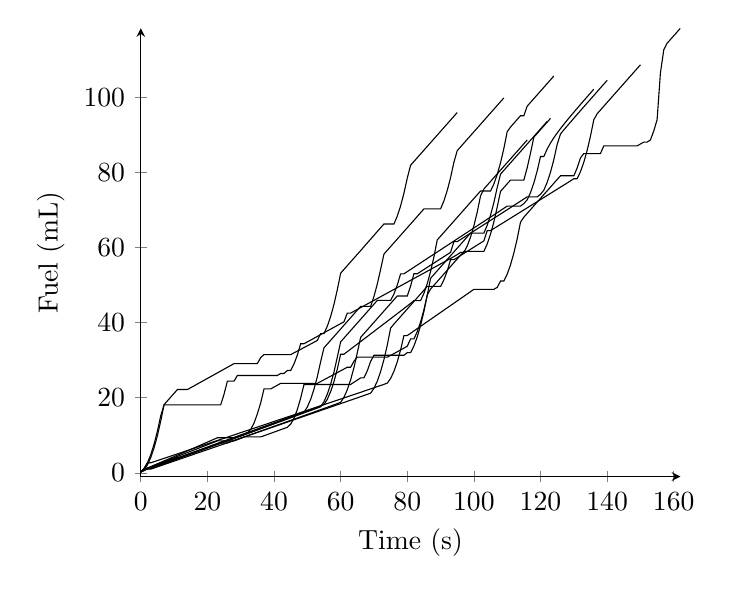
\begin{tikzpicture}
\begin{axis}[
legend style={anchor=west},
axis x line=bottom,
axis y line=left,
ymin=-1,
xlabel=Time (s),
ylabel=Fuel (mL),
]
\addplot[] coordinates {
(0, 0.239885513361)
(1, 0.766617621116)
(2, 1.08709758181)
(3, 1.40758497837)
(4, 1.72808020027)
(5, 2.04858366472)
(6, 2.36909581918)
(7, 2.68961714422)
(8, 3.01014815659)
(9, 3.33068941274)
(10, 3.6512415127)
(11, 3.97180510443)
(12, 4.29238088878)
(13, 4.61296962496)
(14, 4.93357213677)
(15, 5.25418931972)
(16, 5.57482214894)
(17, 5.89547168835)
(18, 6.21613910102)
(19, 6.53682566105)
(20, 6.85753276724)
(21, 7.17826195881)
(22, 7.49901493359)
(23, 7.81979356912)
(24, 8.14059994722)
(25, 8.46143638284)
(26, 8.78230545781)
(27, 9.10453591631)
(28, 9.4276709852)
(29, 9.75116298729)
(30, 10.0737554582)
(31, 10.3963723276)
(32, 10.7190161515)
(33, 11.04168986)
(34, 11.3643968287)
(35, 11.6871409684)
(36, 12.0099268366)
(37, 12.3327597795)
(38, 12.655646113)
(39, 12.978593358)
(40, 13.3016105483)
(41, 13.6247086404)
(42, 13.9479010682)
(43, 14.2712045075)
(44, 14.5946399521)
(45, 14.918234265)
(46, 15.2420224816)
(47, 15.5660513463)
(48, 15.8903849693)
(49, 16.2151143487)
(50, 16.5403744605)
(51, 16.8663776308)
(52, 17.1934867013)
(53, 17.522405092)
(54, 17.8548280695)
(55, 18.1973707627)
(56, 19.595563849)
(57, 21.6312611565)
(58, 24.3053215731)
(59, 27.6250572516)
(60, 31.6042336095)
(61, 31.6042336095)
(62, 32.2792361189)
(63, 32.9542416009)
(64, 33.6292505828)
(65, 34.3042637193)
(66, 34.9792818336)
(67, 35.6543059721)
(68, 36.3293374845)
(69, 37.0043781377)
(70, 37.6794302852)
(71, 38.3544971234)
(72, 39.029583091)
(73, 39.7046945116)
(74, 40.3798406682)
(75, 41.0557239752)
(76, 41.732784354)
(77, 42.4108338501)
(78, 43.0904833237)
(79, 43.7729239316)
(80, 44.4607689175)
(81, 45.1608350129)
(82, 45.8944650363)
(83, 45.8944650363)
(84, 45.8944650363)
(85, 47.8396063179)
(86, 50.422594991)
(87, 53.6498255499)
(88, 57.534145754)
(89, 62.0576642363)
(90, 63.0616540993)
(91, 64.0656439623)
(92, 65.0696338253)
(93, 66.0736236884)
(94, 67.0776135514)
(95, 68.0816034144)
(96, 69.0855932774)
(97, 70.0895831405)
(98, 71.0935730035)
(99, 72.0975628665)
(100, 73.1015527295)
(101, 74.1055425925)
(102, 75.1095324556)
(103, 75.1095324556)
(104, 75.1095324556)
(105, 75.1095324556)
(106, 76.978263322)
(107, 79.4845079301)
(108, 82.6338864636)
(109, 86.4384723714)
(110, 90.9167923671)
(111, 92.1580150926)
(112, 93.1620049556)
(113, 94.1659948186)
(114, 95.1699846817)
(115, 95.1699846817)
(116, 97.7152725592)
(117, 98.7192624222)
(118, 99.7232522853)
(119, 100.727242148)
(120, 101.731232011)
(121, 102.735221874)
(122, 103.739211737)
(123, 104.7432016)
(124, 105.747191463)
};
\addplot[] coordinates {
(0, 0.239885513361)
(1, 0.721796247693)
(2, 1.0358082283)
(3, 1.34982637617)
(4, 1.66385098473)
(5, 1.97788236635)
(6, 2.29192085391)
(7, 2.60596680255)
(8, 2.92002059156)
(9, 3.23408262644)
(10, 3.54815334123)
(11, 3.8622332011)
(12, 4.17632270518)
(13, 4.49042238972)
(14, 4.80453283163)
(15, 5.11865465244)
(16, 5.43278852269)
(17, 5.74693516691)
(18, 6.06109536916)
(19, 6.37526997933)
(20, 6.68945992023)
(21, 7.0036661956)
(22, 7.31788989928)
(23, 7.63213222558)
(24, 7.94639448118)
(25, 7.94639448118)
(26, 7.94639448118)
(27, 8.27747161143)
(28, 8.59219066325)
(29, 8.90742530016)
(30, 9.22370449251)
(31, 9.54064186901)
(32, 9.85737353126)
(33, 10.1737064241)
(34, 10.4900600247)
(35, 10.8064363194)
(36, 11.1228375603)
(37, 11.4392663111)
(38, 11.7557255038)
(39, 12.072218509)
(40, 12.3887492212)
(41, 12.7053221678)
(42, 13.0219426446)
(43, 13.3386168902)
(44, 13.6553523102)
(45, 13.9721577711)
(46, 14.2890439889)
(47, 14.6060240543)
(48, 14.9231141531)
(49, 15.2403345763)
(50, 15.5577111711)
(51, 15.8752774856)
(52, 16.1930780482)
(53, 16.5111735901)
(54, 16.8296497965)
(55, 17.1486329395)
(56, 17.4683202589)
(57, 17.7890462403)
(58, 18.11145389)
(59, 18.4370782708)
(60, 18.7718404678)
(61, 20.132860248)
(62, 22.131532813)
(63, 24.7683418673)
(64, 28.0502243804)
(65, 31.9905705868)
(66, 36.0839399334)
(67, 37.0879297965)
(68, 38.0919196595)
(69, 39.0959095225)
(70, 40.0998993855)
(71, 41.1038892486)
(72, 42.1078791116)
(73, 43.1118689746)
(74, 44.1158588376)
(75, 45.1198487006)
(76, 46.1238385637)
(77, 47.1278284267)
(78, 47.1278284267)
(79, 47.1278284267)
(80, 47.1278284267)
(81, 49.7619304093)
(82, 53.041062953)
(83, 53.041062953)
(84, 53.6124281296)
(85, 54.1837933355)
(86, 54.7551585738)
(87, 55.3265238478)
(88, 55.8978891615)
(89, 56.4692545192)
(90, 57.0406742607)
(91, 57.6120547424)
(92, 58.1834268074)
(93, 58.754798918)
(94, 61.6018599133)
(95, 61.6018599133)
(96, 62.1690141416)
(97, 62.7361859918)
(98, 63.3033783496)
(99, 63.8705947484)
(100, 64.4378395577)
(101, 65.0051182398)
(102, 65.5724377052)
(103, 66.1398068138)
(104, 66.7072370948)
(105, 67.2747438028)
(106, 67.8423475078)
(107, 68.4100765519)
(108, 68.9779709701)
(109, 69.5460889807)
(110, 70.1145181976)
(111, 70.6833960192)
(112, 71.2529490718)
(113, 71.8235756346)
(114, 72.3954060082)
(115, 72.9721206516)
(116, 73.555576238)
(117, 73.555576238)
(118, 73.555576238)
(119, 73.555576238)
(120, 74.2240216111)
(121, 75.3210347799)
(122, 77.398241346)
(123, 80.1140910005)
(124, 83.4763164865)
(125, 87.4991038124)
(126, 90.3186177379)
(127, 91.3829197557)
(128, 92.4304792154)
(129, 93.4660854342)
(130, 94.4930927181)
(131, 95.5138796674)
(132, 96.5301485974)
(133, 97.5431261577)
(134, 98.5537007135)
(135, 99.5625180369)
(136, 100.570048844)
(137, 101.576636944)
(138, 102.582533827)
(139, 103.587923657)
(140, 104.596899343)
};
\addplot[] coordinates {
(0, 0.239885513361)
(1, 0.841669203293)
(2, 1.17158097305)
(3, 1.50150231265)
(4, 1.83143379257)
(5, 2.16137602963)
(6, 2.49132969183)
(7, 2.82129550378)
(8, 3.15127425287)
(9, 3.48126679619)
(10, 3.81127406847)
(11, 4.14129709111)
(12, 4.14129709111)
(13, 4.47093324678)
(14, 4.80057872468)
(15, 5.130234237)
(16, 5.45990057065)
(17, 5.78957859733)
(18, 6.11926928537)
(19, 6.44897371352)
(20, 6.77869308723)
(21, 7.10842875797)
(22, 7.43818224613)
(23, 7.76795526841)
(24, 8.09903345715)
(25, 8.43193196978)
(26, 8.43193196978)
(27, 8.78943402268)
(28, 9.12186908749)
(29, 9.45431543139)
(30, 9.78677447663)
(31, 10.1192478976)
(32, 10.4517376797)
(33, 10.7842461966)
(34, 11.1167763109)
(35, 11.4493315094)
(36, 11.7819160864)
(37, 12.114535397)
(38, 12.4471962146)
(39, 12.7799072486)
(40, 13.1126799133)
(41, 13.4455295114)
(42, 13.7784771269)
(43, 14.1115528111)
(44, 14.4448012843)
(45, 14.7782930166)
(46, 15.1121483137)
(47, 15.4465990161)
(48, 15.7821949679)
(49, 16.1209905479)
(50, 17.5334240011)
(51, 19.5833105246)
(52, 22.2716527829)
(53, 25.6059067053)
(54, 29.5999814862)
(55, 33.3061568052)
(56, 34.3101466682)
(57, 35.3141365312)
(58, 36.3181263943)
(59, 37.3221162573)
(60, 38.3261061203)
(61, 39.3300959833)
(62, 40.3340858463)
(63, 41.3380757094)
(64, 42.3420655724)
(65, 43.3460554354)
(66, 44.3500452984)
(67, 44.3500452984)
(68, 44.3500452984)
(69, 44.3500452984)
(70, 46.9911366921)
(71, 50.2773696364)
(72, 54.2221775082)
(73, 58.282460115)
(74, 59.2864499781)
(75, 60.2904398411)
(76, 61.2944297041)
(77, 62.2984195671)
(78, 63.3024094302)
(79, 64.3063992932)
(80, 65.3103891562)
(81, 66.3143790192)
(82, 67.3183688823)
(83, 68.3223587453)
(84, 69.3263486083)
(85, 70.3303384713)
(86, 70.3303384713)
(87, 70.3303384713)
(88, 70.3303384713)
(89, 70.3303384713)
(90, 70.3303384713)
(91, 72.4648003665)
(92, 75.2383364436)
(93, 78.659259489)
(94, 82.7423355536)
(95, 85.8598887676)
(96, 86.8638786306)
(97, 87.8678684936)
(98, 88.8718583566)
(99, 89.8758482197)
(100, 90.8798380827)
(101, 91.8838279457)
(102, 92.8878178087)
(103, 93.8918076718)
(104, 94.8957975348)
(105, 95.8997873978)
(106, 96.9037772608)
(107, 97.9077671239)
(108, 98.9117569869)
(109, 99.9157468499)
};
\addplot[] coordinates {
(0, 0.239885513361)
(1, 1.13183007041)
(2, 2.66515136892)
(3, 2.66515136892)
(4, 2.96235257606)
(5, 3.25955820712)
(6, 3.55676843281)
(7, 3.85398343273)
(8, 4.15120339604)
(9, 4.44842852202)
(10, 4.74565902083)
(11, 5.04289511423)
(12, 5.34013703641)
(13, 5.63738503487)
(14, 5.93463937137)
(15, 6.23190032301)
(16, 6.52916818334)
(17, 6.82644326363)
(18, 7.12372589422)
(19, 7.42101642604)
(20, 7.71831523218)
(21, 8.01562270977)
(22, 8.31293928188)
(23, 8.61026539973)
(24, 8.90760154507)
(25, 9.20494823284)
(26, 9.50230601407)
(27, 9.79967547914)
(28, 10.0970572614)
(29, 10.3944520411)
(30, 10.6918605499)
(31, 10.9892835761)
(32, 11.2867219696)
(33, 11.584487037)
(34, 11.8827476291)
(35, 12.1813654198)
(36, 12.480364028)
(37, 12.7791215077)
(38, 13.0778021433)
(39, 13.3764940493)
(40, 13.675198016)
(41, 13.9739149096)
(42, 14.2726456827)
(43, 14.5713913849)
(44, 14.8701531758)
(45, 15.1689323401)
(46, 15.4677303049)
(47, 15.7665486608)
(48, 16.0653891859)
(49, 16.3642538755)
(50, 16.6631449759)
(51, 16.9620650271)
(52, 17.2610169129)
(53, 17.5600039227)
(54, 17.8590298276)
(55, 18.1580989739)
(56, 18.4572164013)
(57, 18.7563879913)
(58, 19.0556206571)
(59, 19.3549225898)
(60, 19.6543035811)
(61, 19.9537754542)
(62, 20.2533526483)
(63, 20.5530530291)
(64, 20.8528990394)
(65, 21.15291938)
(66, 21.4531515465)
(67, 21.7536458203)
(68, 22.0544718671)
(69, 22.3557303682)
(70, 22.6575753117)
(71, 22.9602619193)
(72, 23.2642685836)
(73, 23.5707050723)
(74, 23.8837013296)
(75, 25.1400136243)
(76, 27.0345137512)
(77, 29.5666297562)
(78, 32.7422429499)
(79, 36.5736879078)
(80, 36.5736879078)
(81, 37.1894854606)
(82, 37.8052847332)
(83, 38.4210859741)
(84, 39.0368894804)
(85, 39.6526956109)
(86, 40.2685048014)
(87, 40.8843175871)
(88, 41.5001346311)
(89, 42.1159567648)
(90, 42.7317850424)
(91, 43.3476208197)
(92, 43.963465866)
(93, 44.5793225301)
(94, 45.1951939904)
(95, 45.8110846423)
(96, 46.4270364848)
(97, 47.0439221787)
(98, 47.6612467951)
(99, 48.2792081915)
(100, 48.89813525)
(101, 48.89813525)
(102, 48.89813525)
(103, 48.89813525)
(104, 48.89813525)
(105, 48.89813525)
(106, 48.89813525)
(107, 49.4127215327)
(108, 51.1084813475)
(109, 51.1084813475)
(110, 52.9547626197)
(111, 55.4384772704)
(112, 58.5650180069)
(113, 62.3462308016)
(114, 66.8004148913)
(115, 68.1235435499)
(116, 69.1275334129)
(117, 70.131523276)
(118, 71.135513139)
(119, 72.139503002)
(120, 73.143492865)
(121, 74.1474827281)
(122, 75.1514725911)
(123, 76.1554624541)
(124, 77.1594523171)
(125, 78.1634421802)
(126, 79.1674320432)
(127, 79.1674320432)
(128, 79.1674320432)
(129, 79.1674320432)
(130, 79.1674320432)
(131, 81.2350104653)
(132, 83.9411645953)
(133, 85.0856655006)
(134, 85.0856655006)
(135, 85.0856655006)
(136, 85.0856655006)
(137, 85.0856655006)
(138, 85.0856655006)
(139, 87.1302386009)
(140, 87.1302386009)
(141, 87.1302386009)
(142, 87.1302386009)
(143, 87.1302386009)
(144, 87.1302386009)
(145, 87.1302386009)
(146, 87.1302386009)
(147, 87.1302386009)
(148, 87.1302386009)
(149, 87.1302386009)
(150, 87.6344866857)
(151, 88.1387810755)
(152, 88.1387810755)
(153, 88.7285525069)
(154, 91.1042606744)
(155, 94.1214294934)
(156, 106.573118119)
(157, 112.70473431)
(158, 114.476541069)
(159, 115.480530932)
(160, 116.484520795)
(161, 117.488510658)
(162, 118.492500521)
};
\addplot[] coordinates {
(0, 0.239885513361)
(1, 0.670769182584)
(2, 0.97634956868)
(3, 0.97634956868)
(4, 1.28173702068)
(5, 1.58712693446)
(6, 1.89251941507)
(7, 2.19791457363)
(8, 2.5033125278)
(9, 2.80871340223)
(10, 3.11411732915)
(11, 3.4195244489)
(12, 3.72493491058)
(13, 4.03034887276)
(14, 4.33576650425)
(15, 4.64118798492)
(16, 4.94661350664)
(17, 5.25204327429)
(18, 5.5574775069)
(19, 5.86291643891)
(20, 6.16836032151)
(21, 6.47380942422)
(22, 6.77926403658)
(23, 7.08472447004)
(24, 7.39019106012)
(25, 7.69566416876)
(26, 8.001144187)
(27, 8.30663153799)
(28, 8.61212668037)
(29, 8.9176301121)
(30, 9.22314237479)
(31, 9.52866405863)
(32, 9.83419580801)
(33, 10.1405566481)
(34, 10.4475696363)
(35, 10.7551515939)
(36, 11.0626101217)
(37, 11.3697363697)
(38, 11.6768674172)
(39, 11.9840036593)
(40, 12.2911455359)
(41, 12.5982935385)
(42, 12.9054482185)
(43, 13.2126101959)
(44, 13.5197801716)
(45, 13.8269589402)
(46, 14.1341474068)
(47, 14.4413466077)
(48, 14.7485577349)
(49, 15.0557821674)
(50, 15.3630215103)
(51, 15.6702776442)
(52, 15.9775527885)
(53, 16.2848495839)
(54, 16.5921712007)
(55, 16.8995214837)
(56, 17.206905149)
(57, 17.5143280581)
(58, 17.8217976068)
(59, 18.1293232937)
(60, 18.4369175789)
(61, 18.7445972328)
(62, 19.0523855609)
(63, 19.3603163109)
(64, 19.6684411138)
(65, 19.9768453387)
(66, 20.2856878897)
(67, 20.5953316392)
(68, 20.9070759547)
(69, 21.2222070277)
(70, 22.5016131427)
(71, 24.4190743231)
(72, 26.9742512933)
(73, 30.1732580424)
(74, 34.0286618246)
(75, 38.5594831588)
(76, 39.6365881465)
(77, 40.6405780095)
(78, 41.6445678725)
(79, 42.6485577356)
(80, 43.6525475986)
(81, 44.6565374616)
(82, 45.6605273246)
(83, 46.6645171877)
(84, 47.6685070507)
(85, 48.6724969137)
(86, 49.6764867767)
(87, 49.6764867767)
(88, 49.6764867767)
(89, 49.6764867767)
(90, 49.6764867767)
(91, 51.413532691)
(92, 53.7877354245)
(93, 56.8033810707)
(94, 56.8033810707)
(95, 57.3587054684)
(96, 57.914030616)
(97, 58.4693565872)
(98, 59.0246834657)
(99, 59.5800113466)
(100, 60.1353403387)
(101, 60.6907425922)
(102, 61.2460821515)
(103, 61.8014232753)
(104, 64.5476058339)
(105, 64.5476058339)
(106, 65.0990555305)
(107, 65.650508463)
(108, 66.2019651102)
(109, 66.7534260481)
(110, 67.3048919746)
(111, 67.8563637437)
(112, 68.4078424104)
(113, 68.9593292917)
(114, 69.5108260517)
(115, 70.0623348211)
(116, 70.6138583682)
(117, 71.1654003496)
(118, 71.716965687)
(119, 72.2685611476)
(120, 72.8201962676)
(121, 73.371884877)
(122, 73.9236477226)
(123, 74.4755172155)
(124, 75.0275465627)
(125, 75.5798287059)
(126, 76.1324848557)
(127, 76.6859794371)
(128, 77.2411791602)
(129, 77.8009731661)
(130, 78.3807087889)
(131, 78.3807087889)
(132, 80.2519865043)
(133, 82.760787585)
(134, 85.9127580223)
(135, 89.7199970722)
(136, 94.1021001543)
(137, 95.6943595191)
(138, 96.6983493821)
(139, 97.7023392451)
(140, 98.7063291081)
(141, 99.7103189712)
(142, 100.714308834)
(143, 101.718298697)
(144, 102.72228856)
(145, 103.726278423)
(146, 104.730268286)
(147, 105.734258149)
(148, 106.738248012)
(149, 107.742237875)
(150, 108.746227738)
};
\addplot[] coordinates {
(0, 0.239885513361)
(1, 0.777249275829)
(2, 1.09916109643)
(3, 1.09916109643)
(4, 1.42083073583)
(5, 1.74250449665)
(6, 2.06418260723)
(7, 2.38586531317)
(8, 2.70755287895)
(9, 3.02924558978)
(10, 3.35094375371)
(11, 3.67264770398)
(12, 3.99435780158)
(13, 4.31607443831)
(14, 4.63779804008)
(15, 4.95952907074)
(16, 5.28126803643)
(17, 5.60301549053)
(18, 5.92477203929)
(19, 6.24653834839)
(20, 6.56831515041)
(21, 6.89010325348)
(22, 7.21190355137)
(23, 7.53371703518)
(24, 7.85554480707)
(25, 8.17738809635)
(26, 8.49964170991)
(27, 8.82363175312)
(28, 9.14855358767)
(29, 9.47292146148)
(30, 9.7967562352)
(31, 10.1205993543)
(32, 10.4444517281)
(33, 10.7683144046)
(34, 11.092188598)
(35, 11.4160757233)
(36, 11.7399774405)
(37, 12.063895711)
(38, 12.3878328698)
(39, 12.7117917215)
(40, 13.0357756666)
(41, 13.3597888728)
(42, 13.6838365106)
(43, 14.0079250838)
(44, 14.3320629048)
(45, 14.656260798)
(46, 14.980533174)
(47, 15.3048997392)
(48, 15.6293883526)
(49, 15.9540401062)
(50, 16.2789191321)
(51, 16.6041337774)
(52, 16.9298904791)
(53, 17.2566728275)
(54, 17.586263063)
(55, 18.949459745)
(56, 20.9502999127)
(57, 23.5892892364)
(58, 26.873386651)
(59, 30.8160043567)
(60, 34.8925074388)
(61, 35.8964973018)
(62, 36.9004871648)
(63, 37.9044770279)
(64, 38.9084668909)
(65, 39.9124567539)
(66, 40.9164466169)
(67, 41.92043648)
(68, 42.924426343)
(69, 43.928416206)
(70, 44.932406069)
(71, 45.936395932)
(72, 45.936395932)
(73, 45.936395932)
(74, 45.936395932)
(75, 45.936395932)
(76, 47.6641271901)
(77, 50.029000469)
(78, 53.0352075251)
(79, 53.0352075251)
(80, 53.6168144616)
(81, 54.1984223644)
(82, 54.780031339)
(83, 55.3616415068)
(84, 55.9432530078)
(85, 56.5249400445)
(86, 57.1065719349)
(87, 57.6881971597)
(88, 58.2698245781)
(89, 58.8516760992)
(90, 59.4333349549)
(91, 60.014997971)
(92, 60.596665832)
(93, 61.1783393771)
(94, 61.7600196447)
(95, 62.3417079339)
(96, 62.9234058898)
(97, 63.5051156238)
(98, 64.0868398857)
(99, 64.6685823181)
(100, 65.2503478381)
(101, 65.8321432289)
(102, 66.4139780839)
(103, 66.9958663721)
(104, 67.5778291433)
(105, 68.1598994518)
(106, 68.7421318834)
(107, 69.3246224531)
(108, 69.9075544174)
(109, 70.4912375548)
(110, 71.0767812554)
(111, 71.0767812554)
(112, 71.0767812554)
(113, 71.0767812554)
(114, 71.0767812554)
(115, 71.7536799432)
(116, 72.7557925884)
(117, 74.6780304866)
(118, 77.2380060142)
(119, 80.4418815665)
(120, 84.3022728038)
(121, 84.3022728038)
(122, 86.2992025034)
(123, 87.9028200714)
(124, 89.2947124505)
(125, 90.5602805216)
(126, 91.7455207615)
(127, 92.8774548978)
(128, 93.9729446596)
(129, 95.0429816874)
(130, 96.0949662386)
(131, 97.1340020973)
(132, 98.1636732279)
(133, 99.1865305011)
(134, 100.20440785)
(135, 101.221816107)
(136, 102.260816814)
};
\addplot[] coordinates {
(0, 0.239885513361)
(1, 0.573875905005)
(2, 1.15496767622)
(3, 1.55393223668)
(4, 2.01479615362)
(5, 2.39798838878)
(6, 2.78119837679)
(7, 3.1644281472)
(8, 3.54768005017)
(9, 3.93095682223)
(10, 4.31426166895)
(11, 4.69759836973)
(12, 5.08097141201)
(13, 5.46438616503)
(14, 5.84784910726)
(15, 6.23136812838)
(16, 6.61651710011)
(17, 7.01086030938)
(18, 7.40013707314)
(19, 7.78712181789)
(20, 8.17414954092)
(21, 8.5612307338)
(22, 8.94837960508)
(23, 9.33561589681)
(24, 9.33561589681)
(25, 9.33561589681)
(26, 9.33561589681)
(27, 9.33561589681)
(28, 9.33561589681)
(29, 9.66873214584)
(30, 10.002470679)
(31, 10.3372177663)
(32, 10.6745889968)
(33, 11.5401970537)
(34, 13.2600860483)
(35, 15.7080374648)
(36, 18.6336858649)
(37, 22.3512890668)
(38, 22.3512890668)
(39, 22.3512890668)
(40, 22.8459874148)
(41, 23.3406883628)
(42, 23.8353921333)
(43, 23.8353921333)
(44, 23.8353921333)
(45, 23.8353921333)
(46, 23.8353921333)
(47, 23.8353921333)
(48, 23.8353921333)
(49, 23.8353921333)
(50, 23.8353921333)
(51, 23.8353921333)
(52, 23.8353921333)
(53, 23.8353921333)
(54, 24.3133636338)
(55, 24.7913510127)
(56, 25.2693516809)
(57, 25.7473652079)
(58, 26.2253923298)
(59, 26.7034345163)
(60, 27.1814938137)
(61, 27.6595728317)
(62, 28.1376748193)
(63, 28.1376748193)
(64, 29.7273615985)
(65, 30.816180488)
(66, 30.816180488)
(67, 30.816180488)
(68, 30.816180488)
(69, 30.816180488)
(70, 30.816180488)
(71, 30.816180488)
(72, 30.816180488)
(73, 30.816180488)
(74, 30.816180488)
(75, 31.2951668338)
(76, 31.7748334345)
(77, 32.2555191994)
(78, 32.7378374968)
(79, 33.224828662)
(80, 33.7285893298)
(81, 35.675716497)
(82, 35.675716497)
(83, 37.620338255)
(84, 40.2028048221)
(85, 43.429505428)
(86, 47.3132825672)
(87, 51.8411049818)
(88, 52.8450948448)
(89, 53.8490847078)
(90, 54.8530745708)
(91, 55.8570644339)
(92, 56.8610542969)
(93, 57.8650441599)
(94, 58.8690340229)
(95, 59.873023886)
(96, 60.877013749)
(97, 61.881003612)
(98, 62.884993475)
(99, 63.888983338)
(100, 63.888983338)
(101, 63.888983338)
(102, 63.888983338)
(103, 63.888983338)
(104, 65.9582563257)
(105, 68.6661167734)
(106, 72.0202170416)
(107, 76.0346627557)
(108, 79.6003740644)
(109, 80.6043639275)
(110, 81.6083537905)
(111, 82.6123436535)
(112, 83.6163335165)
(113, 84.6203233796)
(114, 85.6243132426)
(115, 86.6283031056)
(116, 87.6322929686)
(117, 88.6362828316)
(118, 89.6402726947)
(119, 90.6442625577)
(120, 91.6482524207)
(121, 92.6522422837)
(122, 93.6562321468)
};
\addplot[] coordinates {
(0, 0.239885513361)
(1, 0.954978135027)
(2, 1.29683412691)
(3, 1.63870293383)
(4, 1.98058544256)
(5, 2.32248262373)
(6, 2.66439554202)
(7, 3.00632536789)
(8, 3.348273391)
(9, 3.6902410359)
(10, 4.03222988013)
(11, 4.37424167545)
(12, 4.71627837255)
(13, 5.05834215031)
(14, 5.40043545022)
(15, 5.74256101736)
(16, 6.08472194933)
(17, 6.42692175493)
(18, 6.76916442512)
(19, 7.11145451924)
(20, 7.45379727057)
(21, 7.79717646909)
(22, 8.14314571515)
(23, 8.48944596301)
(24, 8.48944596301)
(25, 8.48944596301)
(26, 8.48944596301)
(27, 8.48944596301)
(28, 8.48944596301)
(29, 8.84547992202)
(30, 9.20152092991)
(31, 9.55759703252)
(32, 9.55759703252)
(33, 9.55759703252)
(34, 9.55759703252)
(35, 9.55759703252)
(36, 9.55759703252)
(37, 9.87755737656)
(38, 10.197696477)
(39, 10.5179981205)
(40, 10.8385062997)
(41, 11.1593104723)
(42, 11.4805812723)
(43, 11.802706969)
(44, 12.1270503677)
(45, 12.9719338416)
(46, 14.5244781328)
(47, 16.8836483577)
(48, 19.8840863198)
(49, 23.5363793679)
(50, 23.5363793679)
(51, 23.5363793679)
(52, 23.5363793679)
(53, 23.5363793679)
(54, 23.5363793679)
(55, 23.5363793679)
(56, 23.5363793679)
(57, 23.5363793679)
(58, 23.5363793679)
(59, 23.5363793679)
(60, 23.5363793679)
(61, 23.5363793679)
(62, 23.5363793679)
(63, 23.5363793679)
(64, 24.1262856254)
(65, 24.7162821077)
(66, 25.3063710179)
(67, 25.3063710179)
(68, 27.1744772553)
(69, 29.6800948898)
(70, 31.3282356667)
(71, 31.3282356667)
(72, 31.3282356667)
(73, 31.3282356667)
(74, 31.3282356667)
(75, 31.3282356667)
(76, 31.3282356667)
(77, 31.3282356667)
(78, 31.3282356667)
(79, 31.3282356667)
(80, 32.0208283985)
(81, 32.0208283985)
(82, 33.8059242619)
(83, 36.2282752043)
(84, 39.2926540315)
(85, 43.0102868141)
(86, 47.3988528877)
(87, 48.965469509)
(88, 49.969459372)
(89, 50.9734492351)
(90, 51.9774390981)
(91, 52.9814289611)
(92, 53.9854188241)
(93, 54.9894086872)
(94, 55.9933985502)
(95, 56.9973884132)
(96, 58.0013782762)
(97, 59.0053681393)
(98, 59.0053681393)
(99, 59.0053681393)
(100, 59.0053681393)
(101, 59.0053681393)
(102, 59.0053681393)
(103, 59.0053681393)
(104, 60.9893320848)
(105, 63.6113485427)
(106, 66.87820543)
(107, 70.8031439289)
(108, 75.0120894822)
(109, 76.0160793452)
(110, 77.0200692082)
(111, 78.0240590712)
(112, 78.0240590712)
(113, 78.0240590712)
(114, 78.0240590712)
(115, 78.0240590712)
(116, 81.2879215458)
(117, 85.2097898779)
(118, 89.4420101887)
(119, 90.4460000517)
(120, 91.4499899147)
(121, 92.4539797777)
(122, 93.4579696408)
(123, 94.4619595038)
};
\addplot[] coordinates {
(0, 0.239885513361)
(1, 1.13183007041)
(2, 2.66515136892)
(3, 4.83562037156)
(4, 7.64546130585)
(5, 11.1033516642)
(6, 15.2244222039)
(7, 18.1101790691)
(8, 18.1101790691)
(9, 18.1101790691)
(10, 18.1101790691)
(11, 18.1101790691)
(12, 18.1101790691)
(13, 18.1101790691)
(14, 18.1101790691)
(15, 18.1101790691)
(16, 18.1101790691)
(17, 18.1101790691)
(18, 18.1101790691)
(19, 18.1101790691)
(20, 18.1101790691)
(21, 18.1101790691)
(22, 18.1101790691)
(23, 18.1101790691)
(24, 18.1101790691)
(25, 20.9438611173)
(26, 24.4260385476)
(27, 24.4260385476)
(28, 24.4260385476)
(29, 25.9416404882)
(30, 25.9416404882)
(31, 25.9416404882)
(32, 25.9416404882)
(33, 25.9416404882)
(34, 25.9416404882)
(35, 25.9416404882)
(36, 25.9416404882)
(37, 25.9416404882)
(38, 25.9416404882)
(39, 25.9416404882)
(40, 25.9416404882)
(41, 25.9416404882)
(42, 26.4711136378)
(43, 26.4711136378)
(44, 27.2663384728)
(45, 27.2663384728)
(46, 29.0032521913)
(47, 31.3773225091)
(48, 34.3928341813)
(49, 34.3928341813)
(50, 34.8805264291)
(51, 35.3682186903)
(52, 35.8559109657)
(53, 36.3436032564)
(54, 36.8312955635)
(55, 37.3189878884)
(56, 37.8066802324)
(57, 38.2943725971)
(58, 38.7821008062)
(59, 39.2697981035)
(60, 39.757495418)
(61, 40.2451927512)
(62, 42.5669854804)
(63, 42.5669854804)
(64, 43.0516716423)
(65, 43.536363882)
(66, 44.0210628391)
(67, 44.5057692447)
(68, 44.9904839389)
(69, 45.4752078906)
(70, 45.9599422238)
(71, 46.4446882491)
(72, 46.9294475033)
(73, 47.4142218002)
(74, 47.8990132947)
(75, 48.383824566)
(76, 48.8686587251)
(77, 49.3535195577)
(78, 49.8384117137)
(79, 50.3233409645)
(80, 50.8083145561)
(81, 51.2933417019)
(82, 51.7784342852)
(83, 52.2636078789)
(84, 52.7488832629)
(85, 53.2342887427)
(86, 53.7198638001)
(87, 54.2056650504)
(88, 54.6917763714)
(89, 55.1783269949)
(90, 55.665183629)
(91, 56.1537812453)
(92, 56.643665958)
(93, 57.1365931458)
(94, 57.6358794235)
(95, 58.1519191625)
(96, 58.7421665511)
(97, 58.7421665511)
(98, 60.4634523491)
(99, 62.8218707357)
(100, 65.8215481916)
(101, 69.4730644624)
(102, 73.7934525583)
(103, 75.6457683677)
(104, 76.6497582307)
(105, 77.6537480938)
(106, 78.6577379568)
(107, 79.6617278198)
(108, 80.6657176828)
(109, 81.6697075459)
(110, 82.6736974089)
(111, 83.6776872719)
(112, 84.6816771349)
(113, 85.685666998)
(114, 86.689656861)
(115, 87.693646724)
(116, 88.697636587)
};
\addplot[] coordinates {
(0, 0.239885513361)
(1, 0.770600333171)
(2, 2.09972707916)
(3, 4.06665137892)
(4, 6.6715352084)
(5, 9.92099380841)
(6, 13.8280956846)
(7, 18.1734030458)
(8, 19.1773929088)
(9, 20.1813827718)
(10, 21.1853726348)
(11, 22.1893624979)
(12, 22.1893624979)
(13, 22.1893624979)
(14, 22.1893624979)
(15, 22.6826677054)
(16, 23.1759759944)
(17, 23.6692876433)
(18, 24.162602965)
(19, 24.6559223118)
(20, 25.1492460819)
(21, 25.6425747271)
(22, 26.1359087623)
(23, 26.6292487761)
(24, 27.122595445)
(25, 27.6159495496)
(26, 28.109311996)
(27, 28.6026838407)
(28, 29.0960663236)
(29, 29.0960663236)
(30, 29.0960663236)
(31, 29.0960663236)
(32, 29.0960663236)
(33, 29.0960663236)
(34, 29.0960663236)
(35, 29.0960663236)
(36, 30.7098180123)
(37, 31.5033042858)
(38, 31.5033042858)
(39, 31.5033042858)
(40, 31.5033042858)
(41, 31.5033042858)
(42, 31.5033042858)
(43, 31.5033042858)
(44, 31.5033042858)
(45, 31.5033042858)
(46, 31.9708846323)
(47, 32.4388424862)
(48, 32.9072118679)
(49, 33.3761605978)
(50, 33.8458036103)
(51, 34.3175048259)
(52, 34.7936775789)
(53, 35.2860259332)
(54, 37.0946259776)
(55, 37.0946259776)
(56, 39.053561759)
(57, 41.6504150686)
(58, 44.8917201928)
(59, 48.7904646826)
(60, 53.2006189129)
(61, 54.2046087759)
(62, 55.2085986389)
(63, 56.2125885019)
(64, 57.216578365)
(65, 58.220568228)
(66, 59.2183237393)
(67, 60.2385767083)
(68, 61.2544570662)
(69, 62.2671511642)
(70, 63.277518558)
(71, 64.3043019317)
(72, 65.3082917948)
(73, 66.3122816578)
(74, 66.3122816578)
(75, 66.3122816578)
(76, 66.3122816578)
(77, 68.4006221927)
(78, 71.1276855705)
(79, 74.5013173405)
(80, 78.5358163165)
(81, 81.9666063863)
(82, 82.9705962493)
(83, 83.9745861123)
(84, 84.9785759753)
(85, 85.9825658383)
(86, 86.9865557014)
(87, 87.9905455644)
(88, 88.9945354274)
(89, 89.9985252904)
(90, 91.0025151535)
(91, 92.0065050165)
(92, 93.0104948795)
(93, 94.0144847425)
(94, 95.0184746056)
(95, 96.0224644686)
};

\end{axis}
\end{tikzpicture}
\label{tik:fuel:100:51}
\caption{100 percent diving with GSC on route $51$}
\end{figure}

%
\begin{figure}
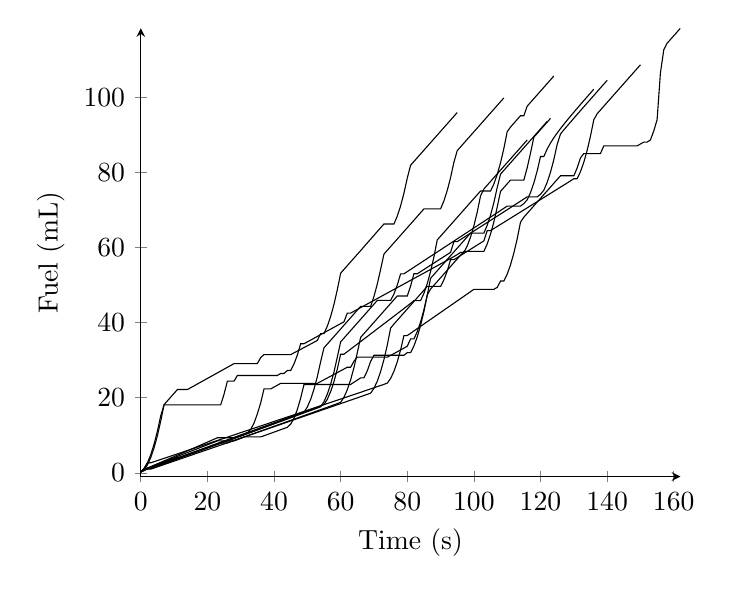
\begin{tikzpicture}
\begin{axis}[
legend style={anchor=west},
axis x line=bottom,
axis y line=left,
ymin=-1,
xlabel=Time (s),
ylabel=Fuel (mL),
]
\addplot[] coordinates {
(0, 0.239885513361)
(1, 0.766617621116)
(2, 1.08709758181)
(3, 1.40758497837)
(4, 1.72808020027)
(5, 2.04858366472)
(6, 2.36909581918)
(7, 2.68961714422)
(8, 3.01014815659)
(9, 3.33068941274)
(10, 3.6512415127)
(11, 3.97180510443)
(12, 4.29238088878)
(13, 4.61296962496)
(14, 4.93357213677)
(15, 5.25418931972)
(16, 5.57482214894)
(17, 5.89547168835)
(18, 6.21613910102)
(19, 6.53682566105)
(20, 6.85753276724)
(21, 7.17826195881)
(22, 7.49901493359)
(23, 7.81979356912)
(24, 8.14059994722)
(25, 8.46143638284)
(26, 8.78230545781)
(27, 9.10453591631)
(28, 9.4276709852)
(29, 9.75116298729)
(30, 10.0737554582)
(31, 10.3963723276)
(32, 10.7190161515)
(33, 11.04168986)
(34, 11.3643968287)
(35, 11.6871409684)
(36, 12.0099268366)
(37, 12.3327597795)
(38, 12.655646113)
(39, 12.978593358)
(40, 13.3016105483)
(41, 13.6247086404)
(42, 13.9479010682)
(43, 14.2712045075)
(44, 14.5946399521)
(45, 14.918234265)
(46, 15.2420224816)
(47, 15.5660513463)
(48, 15.8903849693)
(49, 16.2151143487)
(50, 16.5403744605)
(51, 16.8663776308)
(52, 17.1934867013)
(53, 17.522405092)
(54, 17.8548280695)
(55, 18.1973707627)
(56, 19.595563849)
(57, 21.6312611565)
(58, 24.3053215731)
(59, 27.6250572516)
(60, 31.6042336095)
(61, 31.6042336095)
(62, 32.2792361189)
(63, 32.9542416009)
(64, 33.6292505828)
(65, 34.3042637193)
(66, 34.9792818336)
(67, 35.6543059721)
(68, 36.3293374845)
(69, 37.0043781377)
(70, 37.6794302852)
(71, 38.3544971234)
(72, 39.029583091)
(73, 39.7046945116)
(74, 40.3798406682)
(75, 41.0557239752)
(76, 41.732784354)
(77, 42.4108338501)
(78, 43.0904833237)
(79, 43.7729239316)
(80, 44.4607689175)
(81, 45.1608350129)
(82, 45.8944650363)
(83, 45.8944650363)
(84, 45.8944650363)
(85, 47.8396063179)
(86, 50.422594991)
(87, 53.6498255499)
(88, 57.534145754)
(89, 62.0576642363)
(90, 63.0616540993)
(91, 64.0656439623)
(92, 65.0696338253)
(93, 66.0736236884)
(94, 67.0776135514)
(95, 68.0816034144)
(96, 69.0855932774)
(97, 70.0895831405)
(98, 71.0935730035)
(99, 72.0975628665)
(100, 73.1015527295)
(101, 74.1055425925)
(102, 75.1095324556)
(103, 75.1095324556)
(104, 75.1095324556)
(105, 75.1095324556)
(106, 76.978263322)
(107, 79.4845079301)
(108, 82.6338864636)
(109, 86.4384723714)
(110, 90.9167923671)
(111, 92.1580150926)
(112, 93.1620049556)
(113, 94.1659948186)
(114, 95.1699846817)
(115, 95.1699846817)
(116, 97.7152725592)
(117, 98.7192624222)
(118, 99.7232522853)
(119, 100.727242148)
(120, 101.731232011)
(121, 102.735221874)
(122, 103.739211737)
(123, 104.7432016)
(124, 105.747191463)
};
\addplot[] coordinates {
(0, 0.239885513361)
(1, 0.721796247693)
(2, 1.0358082283)
(3, 1.34982637617)
(4, 1.66385098473)
(5, 1.97788236635)
(6, 2.29192085391)
(7, 2.60596680255)
(8, 2.92002059156)
(9, 3.23408262644)
(10, 3.54815334123)
(11, 3.8622332011)
(12, 4.17632270518)
(13, 4.49042238972)
(14, 4.80453283163)
(15, 5.11865465244)
(16, 5.43278852269)
(17, 5.74693516691)
(18, 6.06109536916)
(19, 6.37526997933)
(20, 6.68945992023)
(21, 7.0036661956)
(22, 7.31788989928)
(23, 7.63213222558)
(24, 7.94639448118)
(25, 7.94639448118)
(26, 7.94639448118)
(27, 8.27747161143)
(28, 8.59219066325)
(29, 8.90742530016)
(30, 9.22370449251)
(31, 9.54064186901)
(32, 9.85737353126)
(33, 10.1737064241)
(34, 10.4900600247)
(35, 10.8064363194)
(36, 11.1228375603)
(37, 11.4392663111)
(38, 11.7557255038)
(39, 12.072218509)
(40, 12.3887492212)
(41, 12.7053221678)
(42, 13.0219426446)
(43, 13.3386168902)
(44, 13.6553523102)
(45, 13.9721577711)
(46, 14.2890439889)
(47, 14.6060240543)
(48, 14.9231141531)
(49, 15.2403345763)
(50, 15.5577111711)
(51, 15.8752774856)
(52, 16.1930780482)
(53, 16.5111735901)
(54, 16.8296497965)
(55, 17.1486329395)
(56, 17.4683202589)
(57, 17.7890462403)
(58, 18.11145389)
(59, 18.4370782708)
(60, 18.7718404678)
(61, 20.132860248)
(62, 22.131532813)
(63, 24.7683418673)
(64, 28.0502243804)
(65, 31.9905705868)
(66, 36.0839399334)
(67, 37.0879297965)
(68, 38.0919196595)
(69, 39.0959095225)
(70, 40.0998993855)
(71, 41.1038892486)
(72, 42.1078791116)
(73, 43.1118689746)
(74, 44.1158588376)
(75, 45.1198487006)
(76, 46.1238385637)
(77, 47.1278284267)
(78, 47.1278284267)
(79, 47.1278284267)
(80, 47.1278284267)
(81, 49.7619304093)
(82, 53.041062953)
(83, 53.041062953)
(84, 53.6124281296)
(85, 54.1837933355)
(86, 54.7551585738)
(87, 55.3265238478)
(88, 55.8978891615)
(89, 56.4692545192)
(90, 57.0406742607)
(91, 57.6120547424)
(92, 58.1834268074)
(93, 58.754798918)
(94, 61.6018599133)
(95, 61.6018599133)
(96, 62.1690141416)
(97, 62.7361859918)
(98, 63.3033783496)
(99, 63.8705947484)
(100, 64.4378395577)
(101, 65.0051182398)
(102, 65.5724377052)
(103, 66.1398068138)
(104, 66.7072370948)
(105, 67.2747438028)
(106, 67.8423475078)
(107, 68.4100765519)
(108, 68.9779709701)
(109, 69.5460889807)
(110, 70.1145181976)
(111, 70.6833960192)
(112, 71.2529490718)
(113, 71.8235756346)
(114, 72.3954060082)
(115, 72.9721206516)
(116, 73.555576238)
(117, 73.555576238)
(118, 73.555576238)
(119, 73.555576238)
(120, 74.2240216111)
(121, 75.3210347799)
(122, 77.398241346)
(123, 80.1140910005)
(124, 83.4763164865)
(125, 87.4991038124)
(126, 90.3186177379)
(127, 91.3829197557)
(128, 92.4304792154)
(129, 93.4660854342)
(130, 94.4930927181)
(131, 95.5138796674)
(132, 96.5301485974)
(133, 97.5431261577)
(134, 98.5537007135)
(135, 99.5625180369)
(136, 100.570048844)
(137, 101.576636944)
(138, 102.582533827)
(139, 103.587923657)
(140, 104.596899343)
};
\addplot[] coordinates {
(0, 0.239885513361)
(1, 0.841669203293)
(2, 1.17158097305)
(3, 1.50150231265)
(4, 1.83143379257)
(5, 2.16137602963)
(6, 2.49132969183)
(7, 2.82129550378)
(8, 3.15127425287)
(9, 3.48126679619)
(10, 3.81127406847)
(11, 4.14129709111)
(12, 4.14129709111)
(13, 4.47093324678)
(14, 4.80057872468)
(15, 5.130234237)
(16, 5.45990057065)
(17, 5.78957859733)
(18, 6.11926928537)
(19, 6.44897371352)
(20, 6.77869308723)
(21, 7.10842875797)
(22, 7.43818224613)
(23, 7.76795526841)
(24, 8.09903345715)
(25, 8.43193196978)
(26, 8.43193196978)
(27, 8.78943402268)
(28, 9.12186908749)
(29, 9.45431543139)
(30, 9.78677447663)
(31, 10.1192478976)
(32, 10.4517376797)
(33, 10.7842461966)
(34, 11.1167763109)
(35, 11.4493315094)
(36, 11.7819160864)
(37, 12.114535397)
(38, 12.4471962146)
(39, 12.7799072486)
(40, 13.1126799133)
(41, 13.4455295114)
(42, 13.7784771269)
(43, 14.1115528111)
(44, 14.4448012843)
(45, 14.7782930166)
(46, 15.1121483137)
(47, 15.4465990161)
(48, 15.7821949679)
(49, 16.1209905479)
(50, 17.5334240011)
(51, 19.5833105246)
(52, 22.2716527829)
(53, 25.6059067053)
(54, 29.5999814862)
(55, 33.3061568052)
(56, 34.3101466682)
(57, 35.3141365312)
(58, 36.3181263943)
(59, 37.3221162573)
(60, 38.3261061203)
(61, 39.3300959833)
(62, 40.3340858463)
(63, 41.3380757094)
(64, 42.3420655724)
(65, 43.3460554354)
(66, 44.3500452984)
(67, 44.3500452984)
(68, 44.3500452984)
(69, 44.3500452984)
(70, 46.9911366921)
(71, 50.2773696364)
(72, 54.2221775082)
(73, 58.282460115)
(74, 59.2864499781)
(75, 60.2904398411)
(76, 61.2944297041)
(77, 62.2984195671)
(78, 63.3024094302)
(79, 64.3063992932)
(80, 65.3103891562)
(81, 66.3143790192)
(82, 67.3183688823)
(83, 68.3223587453)
(84, 69.3263486083)
(85, 70.3303384713)
(86, 70.3303384713)
(87, 70.3303384713)
(88, 70.3303384713)
(89, 70.3303384713)
(90, 70.3303384713)
(91, 72.4648003665)
(92, 75.2383364436)
(93, 78.659259489)
(94, 82.7423355536)
(95, 85.8598887676)
(96, 86.8638786306)
(97, 87.8678684936)
(98, 88.8718583566)
(99, 89.8758482197)
(100, 90.8798380827)
(101, 91.8838279457)
(102, 92.8878178087)
(103, 93.8918076718)
(104, 94.8957975348)
(105, 95.8997873978)
(106, 96.9037772608)
(107, 97.9077671239)
(108, 98.9117569869)
(109, 99.9157468499)
};
\addplot[] coordinates {
(0, 0.239885513361)
(1, 1.13183007041)
(2, 2.66515136892)
(3, 2.66515136892)
(4, 2.96235257606)
(5, 3.25955820712)
(6, 3.55676843281)
(7, 3.85398343273)
(8, 4.15120339604)
(9, 4.44842852202)
(10, 4.74565902083)
(11, 5.04289511423)
(12, 5.34013703641)
(13, 5.63738503487)
(14, 5.93463937137)
(15, 6.23190032301)
(16, 6.52916818334)
(17, 6.82644326363)
(18, 7.12372589422)
(19, 7.42101642604)
(20, 7.71831523218)
(21, 8.01562270977)
(22, 8.31293928188)
(23, 8.61026539973)
(24, 8.90760154507)
(25, 9.20494823284)
(26, 9.50230601407)
(27, 9.79967547914)
(28, 10.0970572614)
(29, 10.3944520411)
(30, 10.6918605499)
(31, 10.9892835761)
(32, 11.2867219696)
(33, 11.584487037)
(34, 11.8827476291)
(35, 12.1813654198)
(36, 12.480364028)
(37, 12.7791215077)
(38, 13.0778021433)
(39, 13.3764940493)
(40, 13.675198016)
(41, 13.9739149096)
(42, 14.2726456827)
(43, 14.5713913849)
(44, 14.8701531758)
(45, 15.1689323401)
(46, 15.4677303049)
(47, 15.7665486608)
(48, 16.0653891859)
(49, 16.3642538755)
(50, 16.6631449759)
(51, 16.9620650271)
(52, 17.2610169129)
(53, 17.5600039227)
(54, 17.8590298276)
(55, 18.1580989739)
(56, 18.4572164013)
(57, 18.7563879913)
(58, 19.0556206571)
(59, 19.3549225898)
(60, 19.6543035811)
(61, 19.9537754542)
(62, 20.2533526483)
(63, 20.5530530291)
(64, 20.8528990394)
(65, 21.15291938)
(66, 21.4531515465)
(67, 21.7536458203)
(68, 22.0544718671)
(69, 22.3557303682)
(70, 22.6575753117)
(71, 22.9602619193)
(72, 23.2642685836)
(73, 23.5707050723)
(74, 23.8837013296)
(75, 25.1400136243)
(76, 27.0345137512)
(77, 29.5666297562)
(78, 32.7422429499)
(79, 36.5736879078)
(80, 36.5736879078)
(81, 37.1894854606)
(82, 37.8052847332)
(83, 38.4210859741)
(84, 39.0368894804)
(85, 39.6526956109)
(86, 40.2685048014)
(87, 40.8843175871)
(88, 41.5001346311)
(89, 42.1159567648)
(90, 42.7317850424)
(91, 43.3476208197)
(92, 43.963465866)
(93, 44.5793225301)
(94, 45.1951939904)
(95, 45.8110846423)
(96, 46.4270364848)
(97, 47.0439221787)
(98, 47.6612467951)
(99, 48.2792081915)
(100, 48.89813525)
(101, 48.89813525)
(102, 48.89813525)
(103, 48.89813525)
(104, 48.89813525)
(105, 48.89813525)
(106, 48.89813525)
(107, 49.4127215327)
(108, 51.1084813475)
(109, 51.1084813475)
(110, 52.9547626197)
(111, 55.4384772704)
(112, 58.5650180069)
(113, 62.3462308016)
(114, 66.8004148913)
(115, 68.1235435499)
(116, 69.1275334129)
(117, 70.131523276)
(118, 71.135513139)
(119, 72.139503002)
(120, 73.143492865)
(121, 74.1474827281)
(122, 75.1514725911)
(123, 76.1554624541)
(124, 77.1594523171)
(125, 78.1634421802)
(126, 79.1674320432)
(127, 79.1674320432)
(128, 79.1674320432)
(129, 79.1674320432)
(130, 79.1674320432)
(131, 81.2350104653)
(132, 83.9411645953)
(133, 85.0856655006)
(134, 85.0856655006)
(135, 85.0856655006)
(136, 85.0856655006)
(137, 85.0856655006)
(138, 85.0856655006)
(139, 87.1302386009)
(140, 87.1302386009)
(141, 87.1302386009)
(142, 87.1302386009)
(143, 87.1302386009)
(144, 87.1302386009)
(145, 87.1302386009)
(146, 87.1302386009)
(147, 87.1302386009)
(148, 87.1302386009)
(149, 87.1302386009)
(150, 87.6344866857)
(151, 88.1387810755)
(152, 88.1387810755)
(153, 88.7285525069)
(154, 91.1042606744)
(155, 94.1214294934)
(156, 106.573118119)
(157, 112.70473431)
(158, 114.476541069)
(159, 115.480530932)
(160, 116.484520795)
(161, 117.488510658)
(162, 118.492500521)
};
\addplot[] coordinates {
(0, 0.239885513361)
(1, 0.670769182584)
(2, 0.97634956868)
(3, 0.97634956868)
(4, 1.28173702068)
(5, 1.58712693446)
(6, 1.89251941507)
(7, 2.19791457363)
(8, 2.5033125278)
(9, 2.80871340223)
(10, 3.11411732915)
(11, 3.4195244489)
(12, 3.72493491058)
(13, 4.03034887276)
(14, 4.33576650425)
(15, 4.64118798492)
(16, 4.94661350664)
(17, 5.25204327429)
(18, 5.5574775069)
(19, 5.86291643891)
(20, 6.16836032151)
(21, 6.47380942422)
(22, 6.77926403658)
(23, 7.08472447004)
(24, 7.39019106012)
(25, 7.69566416876)
(26, 8.001144187)
(27, 8.30663153799)
(28, 8.61212668037)
(29, 8.9176301121)
(30, 9.22314237479)
(31, 9.52866405863)
(32, 9.83419580801)
(33, 10.1405566481)
(34, 10.4475696363)
(35, 10.7551515939)
(36, 11.0626101217)
(37, 11.3697363697)
(38, 11.6768674172)
(39, 11.9840036593)
(40, 12.2911455359)
(41, 12.5982935385)
(42, 12.9054482185)
(43, 13.2126101959)
(44, 13.5197801716)
(45, 13.8269589402)
(46, 14.1341474068)
(47, 14.4413466077)
(48, 14.7485577349)
(49, 15.0557821674)
(50, 15.3630215103)
(51, 15.6702776442)
(52, 15.9775527885)
(53, 16.2848495839)
(54, 16.5921712007)
(55, 16.8995214837)
(56, 17.206905149)
(57, 17.5143280581)
(58, 17.8217976068)
(59, 18.1293232937)
(60, 18.4369175789)
(61, 18.7445972328)
(62, 19.0523855609)
(63, 19.3603163109)
(64, 19.6684411138)
(65, 19.9768453387)
(66, 20.2856878897)
(67, 20.5953316392)
(68, 20.9070759547)
(69, 21.2222070277)
(70, 22.5016131427)
(71, 24.4190743231)
(72, 26.9742512933)
(73, 30.1732580424)
(74, 34.0286618246)
(75, 38.5594831588)
(76, 39.6365881465)
(77, 40.6405780095)
(78, 41.6445678725)
(79, 42.6485577356)
(80, 43.6525475986)
(81, 44.6565374616)
(82, 45.6605273246)
(83, 46.6645171877)
(84, 47.6685070507)
(85, 48.6724969137)
(86, 49.6764867767)
(87, 49.6764867767)
(88, 49.6764867767)
(89, 49.6764867767)
(90, 49.6764867767)
(91, 51.413532691)
(92, 53.7877354245)
(93, 56.8033810707)
(94, 56.8033810707)
(95, 57.3587054684)
(96, 57.914030616)
(97, 58.4693565872)
(98, 59.0246834657)
(99, 59.5800113466)
(100, 60.1353403387)
(101, 60.6907425922)
(102, 61.2460821515)
(103, 61.8014232753)
(104, 64.5476058339)
(105, 64.5476058339)
(106, 65.0990555305)
(107, 65.650508463)
(108, 66.2019651102)
(109, 66.7534260481)
(110, 67.3048919746)
(111, 67.8563637437)
(112, 68.4078424104)
(113, 68.9593292917)
(114, 69.5108260517)
(115, 70.0623348211)
(116, 70.6138583682)
(117, 71.1654003496)
(118, 71.716965687)
(119, 72.2685611476)
(120, 72.8201962676)
(121, 73.371884877)
(122, 73.9236477226)
(123, 74.4755172155)
(124, 75.0275465627)
(125, 75.5798287059)
(126, 76.1324848557)
(127, 76.6859794371)
(128, 77.2411791602)
(129, 77.8009731661)
(130, 78.3807087889)
(131, 78.3807087889)
(132, 80.2519865043)
(133, 82.760787585)
(134, 85.9127580223)
(135, 89.7199970722)
(136, 94.1021001543)
(137, 95.6943595191)
(138, 96.6983493821)
(139, 97.7023392451)
(140, 98.7063291081)
(141, 99.7103189712)
(142, 100.714308834)
(143, 101.718298697)
(144, 102.72228856)
(145, 103.726278423)
(146, 104.730268286)
(147, 105.734258149)
(148, 106.738248012)
(149, 107.742237875)
(150, 108.746227738)
};
\addplot[] coordinates {
(0, 0.239885513361)
(1, 0.777249275829)
(2, 1.09916109643)
(3, 1.09916109643)
(4, 1.42083073583)
(5, 1.74250449665)
(6, 2.06418260723)
(7, 2.38586531317)
(8, 2.70755287895)
(9, 3.02924558978)
(10, 3.35094375371)
(11, 3.67264770398)
(12, 3.99435780158)
(13, 4.31607443831)
(14, 4.63779804008)
(15, 4.95952907074)
(16, 5.28126803643)
(17, 5.60301549053)
(18, 5.92477203929)
(19, 6.24653834839)
(20, 6.56831515041)
(21, 6.89010325348)
(22, 7.21190355137)
(23, 7.53371703518)
(24, 7.85554480707)
(25, 8.17738809635)
(26, 8.49964170991)
(27, 8.82363175312)
(28, 9.14855358767)
(29, 9.47292146148)
(30, 9.7967562352)
(31, 10.1205993543)
(32, 10.4444517281)
(33, 10.7683144046)
(34, 11.092188598)
(35, 11.4160757233)
(36, 11.7399774405)
(37, 12.063895711)
(38, 12.3878328698)
(39, 12.7117917215)
(40, 13.0357756666)
(41, 13.3597888728)
(42, 13.6838365106)
(43, 14.0079250838)
(44, 14.3320629048)
(45, 14.656260798)
(46, 14.980533174)
(47, 15.3048997392)
(48, 15.6293883526)
(49, 15.9540401062)
(50, 16.2789191321)
(51, 16.6041337774)
(52, 16.9298904791)
(53, 17.2566728275)
(54, 17.586263063)
(55, 18.949459745)
(56, 20.9502999127)
(57, 23.5892892364)
(58, 26.873386651)
(59, 30.8160043567)
(60, 34.8925074388)
(61, 35.8964973018)
(62, 36.9004871648)
(63, 37.9044770279)
(64, 38.9084668909)
(65, 39.9124567539)
(66, 40.9164466169)
(67, 41.92043648)
(68, 42.924426343)
(69, 43.928416206)
(70, 44.932406069)
(71, 45.936395932)
(72, 45.936395932)
(73, 45.936395932)
(74, 45.936395932)
(75, 45.936395932)
(76, 47.6641271901)
(77, 50.029000469)
(78, 53.0352075251)
(79, 53.0352075251)
(80, 53.6168144616)
(81, 54.1984223644)
(82, 54.780031339)
(83, 55.3616415068)
(84, 55.9432530078)
(85, 56.5249400445)
(86, 57.1065719349)
(87, 57.6881971597)
(88, 58.2698245781)
(89, 58.8516760992)
(90, 59.4333349549)
(91, 60.014997971)
(92, 60.596665832)
(93, 61.1783393771)
(94, 61.7600196447)
(95, 62.3417079339)
(96, 62.9234058898)
(97, 63.5051156238)
(98, 64.0868398857)
(99, 64.6685823181)
(100, 65.2503478381)
(101, 65.8321432289)
(102, 66.4139780839)
(103, 66.9958663721)
(104, 67.5778291433)
(105, 68.1598994518)
(106, 68.7421318834)
(107, 69.3246224531)
(108, 69.9075544174)
(109, 70.4912375548)
(110, 71.0767812554)
(111, 71.0767812554)
(112, 71.0767812554)
(113, 71.0767812554)
(114, 71.0767812554)
(115, 71.7536799432)
(116, 72.7557925884)
(117, 74.6780304866)
(118, 77.2380060142)
(119, 80.4418815665)
(120, 84.3022728038)
(121, 84.3022728038)
(122, 86.2992025034)
(123, 87.9028200714)
(124, 89.2947124505)
(125, 90.5602805216)
(126, 91.7455207615)
(127, 92.8774548978)
(128, 93.9729446596)
(129, 95.0429816874)
(130, 96.0949662386)
(131, 97.1340020973)
(132, 98.1636732279)
(133, 99.1865305011)
(134, 100.20440785)
(135, 101.221816107)
(136, 102.260816814)
};
\addplot[] coordinates {
(0, 0.239885513361)
(1, 0.573875905005)
(2, 1.15496767622)
(3, 1.55393223668)
(4, 2.01479615362)
(5, 2.39798838878)
(6, 2.78119837679)
(7, 3.1644281472)
(8, 3.54768005017)
(9, 3.93095682223)
(10, 4.31426166895)
(11, 4.69759836973)
(12, 5.08097141201)
(13, 5.46438616503)
(14, 5.84784910726)
(15, 6.23136812838)
(16, 6.61651710011)
(17, 7.01086030938)
(18, 7.40013707314)
(19, 7.78712181789)
(20, 8.17414954092)
(21, 8.5612307338)
(22, 8.94837960508)
(23, 9.33561589681)
(24, 9.33561589681)
(25, 9.33561589681)
(26, 9.33561589681)
(27, 9.33561589681)
(28, 9.33561589681)
(29, 9.66873214584)
(30, 10.002470679)
(31, 10.3372177663)
(32, 10.6745889968)
(33, 11.5401970537)
(34, 13.2600860483)
(35, 15.7080374648)
(36, 18.6336858649)
(37, 22.3512890668)
(38, 22.3512890668)
(39, 22.3512890668)
(40, 22.8459874148)
(41, 23.3406883628)
(42, 23.8353921333)
(43, 23.8353921333)
(44, 23.8353921333)
(45, 23.8353921333)
(46, 23.8353921333)
(47, 23.8353921333)
(48, 23.8353921333)
(49, 23.8353921333)
(50, 23.8353921333)
(51, 23.8353921333)
(52, 23.8353921333)
(53, 23.8353921333)
(54, 24.3133636338)
(55, 24.7913510127)
(56, 25.2693516809)
(57, 25.7473652079)
(58, 26.2253923298)
(59, 26.7034345163)
(60, 27.1814938137)
(61, 27.6595728317)
(62, 28.1376748193)
(63, 28.1376748193)
(64, 29.7273615985)
(65, 30.816180488)
(66, 30.816180488)
(67, 30.816180488)
(68, 30.816180488)
(69, 30.816180488)
(70, 30.816180488)
(71, 30.816180488)
(72, 30.816180488)
(73, 30.816180488)
(74, 30.816180488)
(75, 31.2951668338)
(76, 31.7748334345)
(77, 32.2555191994)
(78, 32.7378374968)
(79, 33.224828662)
(80, 33.7285893298)
(81, 35.675716497)
(82, 35.675716497)
(83, 37.620338255)
(84, 40.2028048221)
(85, 43.429505428)
(86, 47.3132825672)
(87, 51.8411049818)
(88, 52.8450948448)
(89, 53.8490847078)
(90, 54.8530745708)
(91, 55.8570644339)
(92, 56.8610542969)
(93, 57.8650441599)
(94, 58.8690340229)
(95, 59.873023886)
(96, 60.877013749)
(97, 61.881003612)
(98, 62.884993475)
(99, 63.888983338)
(100, 63.888983338)
(101, 63.888983338)
(102, 63.888983338)
(103, 63.888983338)
(104, 65.9582563257)
(105, 68.6661167734)
(106, 72.0202170416)
(107, 76.0346627557)
(108, 79.6003740644)
(109, 80.6043639275)
(110, 81.6083537905)
(111, 82.6123436535)
(112, 83.6163335165)
(113, 84.6203233796)
(114, 85.6243132426)
(115, 86.6283031056)
(116, 87.6322929686)
(117, 88.6362828316)
(118, 89.6402726947)
(119, 90.6442625577)
(120, 91.6482524207)
(121, 92.6522422837)
(122, 93.6562321468)
};
\addplot[] coordinates {
(0, 0.239885513361)
(1, 0.954978135027)
(2, 1.29683412691)
(3, 1.63870293383)
(4, 1.98058544256)
(5, 2.32248262373)
(6, 2.66439554202)
(7, 3.00632536789)
(8, 3.348273391)
(9, 3.6902410359)
(10, 4.03222988013)
(11, 4.37424167545)
(12, 4.71627837255)
(13, 5.05834215031)
(14, 5.40043545022)
(15, 5.74256101736)
(16, 6.08472194933)
(17, 6.42692175493)
(18, 6.76916442512)
(19, 7.11145451924)
(20, 7.45379727057)
(21, 7.79717646909)
(22, 8.14314571515)
(23, 8.48944596301)
(24, 8.48944596301)
(25, 8.48944596301)
(26, 8.48944596301)
(27, 8.48944596301)
(28, 8.48944596301)
(29, 8.84547992202)
(30, 9.20152092991)
(31, 9.55759703252)
(32, 9.55759703252)
(33, 9.55759703252)
(34, 9.55759703252)
(35, 9.55759703252)
(36, 9.55759703252)
(37, 9.87755737656)
(38, 10.197696477)
(39, 10.5179981205)
(40, 10.8385062997)
(41, 11.1593104723)
(42, 11.4805812723)
(43, 11.802706969)
(44, 12.1270503677)
(45, 12.9719338416)
(46, 14.5244781328)
(47, 16.8836483577)
(48, 19.8840863198)
(49, 23.5363793679)
(50, 23.5363793679)
(51, 23.5363793679)
(52, 23.5363793679)
(53, 23.5363793679)
(54, 23.5363793679)
(55, 23.5363793679)
(56, 23.5363793679)
(57, 23.5363793679)
(58, 23.5363793679)
(59, 23.5363793679)
(60, 23.5363793679)
(61, 23.5363793679)
(62, 23.5363793679)
(63, 23.5363793679)
(64, 24.1262856254)
(65, 24.7162821077)
(66, 25.3063710179)
(67, 25.3063710179)
(68, 27.1744772553)
(69, 29.6800948898)
(70, 31.3282356667)
(71, 31.3282356667)
(72, 31.3282356667)
(73, 31.3282356667)
(74, 31.3282356667)
(75, 31.3282356667)
(76, 31.3282356667)
(77, 31.3282356667)
(78, 31.3282356667)
(79, 31.3282356667)
(80, 32.0208283985)
(81, 32.0208283985)
(82, 33.8059242619)
(83, 36.2282752043)
(84, 39.2926540315)
(85, 43.0102868141)
(86, 47.3988528877)
(87, 48.965469509)
(88, 49.969459372)
(89, 50.9734492351)
(90, 51.9774390981)
(91, 52.9814289611)
(92, 53.9854188241)
(93, 54.9894086872)
(94, 55.9933985502)
(95, 56.9973884132)
(96, 58.0013782762)
(97, 59.0053681393)
(98, 59.0053681393)
(99, 59.0053681393)
(100, 59.0053681393)
(101, 59.0053681393)
(102, 59.0053681393)
(103, 59.0053681393)
(104, 60.9893320848)
(105, 63.6113485427)
(106, 66.87820543)
(107, 70.8031439289)
(108, 75.0120894822)
(109, 76.0160793452)
(110, 77.0200692082)
(111, 78.0240590712)
(112, 78.0240590712)
(113, 78.0240590712)
(114, 78.0240590712)
(115, 78.0240590712)
(116, 81.2879215458)
(117, 85.2097898779)
(118, 89.4420101887)
(119, 90.4460000517)
(120, 91.4499899147)
(121, 92.4539797777)
(122, 93.4579696408)
(123, 94.4619595038)
};
\addplot[] coordinates {
(0, 0.239885513361)
(1, 1.13183007041)
(2, 2.66515136892)
(3, 4.83562037156)
(4, 7.64546130585)
(5, 11.1033516642)
(6, 15.2244222039)
(7, 18.1101790691)
(8, 18.1101790691)
(9, 18.1101790691)
(10, 18.1101790691)
(11, 18.1101790691)
(12, 18.1101790691)
(13, 18.1101790691)
(14, 18.1101790691)
(15, 18.1101790691)
(16, 18.1101790691)
(17, 18.1101790691)
(18, 18.1101790691)
(19, 18.1101790691)
(20, 18.1101790691)
(21, 18.1101790691)
(22, 18.1101790691)
(23, 18.1101790691)
(24, 18.1101790691)
(25, 20.9438611173)
(26, 24.4260385476)
(27, 24.4260385476)
(28, 24.4260385476)
(29, 25.9416404882)
(30, 25.9416404882)
(31, 25.9416404882)
(32, 25.9416404882)
(33, 25.9416404882)
(34, 25.9416404882)
(35, 25.9416404882)
(36, 25.9416404882)
(37, 25.9416404882)
(38, 25.9416404882)
(39, 25.9416404882)
(40, 25.9416404882)
(41, 25.9416404882)
(42, 26.4711136378)
(43, 26.4711136378)
(44, 27.2663384728)
(45, 27.2663384728)
(46, 29.0032521913)
(47, 31.3773225091)
(48, 34.3928341813)
(49, 34.3928341813)
(50, 34.8805264291)
(51, 35.3682186903)
(52, 35.8559109657)
(53, 36.3436032564)
(54, 36.8312955635)
(55, 37.3189878884)
(56, 37.8066802324)
(57, 38.2943725971)
(58, 38.7821008062)
(59, 39.2697981035)
(60, 39.757495418)
(61, 40.2451927512)
(62, 42.5669854804)
(63, 42.5669854804)
(64, 43.0516716423)
(65, 43.536363882)
(66, 44.0210628391)
(67, 44.5057692447)
(68, 44.9904839389)
(69, 45.4752078906)
(70, 45.9599422238)
(71, 46.4446882491)
(72, 46.9294475033)
(73, 47.4142218002)
(74, 47.8990132947)
(75, 48.383824566)
(76, 48.8686587251)
(77, 49.3535195577)
(78, 49.8384117137)
(79, 50.3233409645)
(80, 50.8083145561)
(81, 51.2933417019)
(82, 51.7784342852)
(83, 52.2636078789)
(84, 52.7488832629)
(85, 53.2342887427)
(86, 53.7198638001)
(87, 54.2056650504)
(88, 54.6917763714)
(89, 55.1783269949)
(90, 55.665183629)
(91, 56.1537812453)
(92, 56.643665958)
(93, 57.1365931458)
(94, 57.6358794235)
(95, 58.1519191625)
(96, 58.7421665511)
(97, 58.7421665511)
(98, 60.4634523491)
(99, 62.8218707357)
(100, 65.8215481916)
(101, 69.4730644624)
(102, 73.7934525583)
(103, 75.6457683677)
(104, 76.6497582307)
(105, 77.6537480938)
(106, 78.6577379568)
(107, 79.6617278198)
(108, 80.6657176828)
(109, 81.6697075459)
(110, 82.6736974089)
(111, 83.6776872719)
(112, 84.6816771349)
(113, 85.685666998)
(114, 86.689656861)
(115, 87.693646724)
(116, 88.697636587)
};
\addplot[] coordinates {
(0, 0.239885513361)
(1, 0.770600333171)
(2, 2.09972707916)
(3, 4.06665137892)
(4, 6.6715352084)
(5, 9.92099380841)
(6, 13.8280956846)
(7, 18.1734030458)
(8, 19.1773929088)
(9, 20.1813827718)
(10, 21.1853726348)
(11, 22.1893624979)
(12, 22.1893624979)
(13, 22.1893624979)
(14, 22.1893624979)
(15, 22.6826677054)
(16, 23.1759759944)
(17, 23.6692876433)
(18, 24.162602965)
(19, 24.6559223118)
(20, 25.1492460819)
(21, 25.6425747271)
(22, 26.1359087623)
(23, 26.6292487761)
(24, 27.122595445)
(25, 27.6159495496)
(26, 28.109311996)
(27, 28.6026838407)
(28, 29.0960663236)
(29, 29.0960663236)
(30, 29.0960663236)
(31, 29.0960663236)
(32, 29.0960663236)
(33, 29.0960663236)
(34, 29.0960663236)
(35, 29.0960663236)
(36, 30.7098180123)
(37, 31.5033042858)
(38, 31.5033042858)
(39, 31.5033042858)
(40, 31.5033042858)
(41, 31.5033042858)
(42, 31.5033042858)
(43, 31.5033042858)
(44, 31.5033042858)
(45, 31.5033042858)
(46, 31.9708846323)
(47, 32.4388424862)
(48, 32.9072118679)
(49, 33.3761605978)
(50, 33.8458036103)
(51, 34.3175048259)
(52, 34.7936775789)
(53, 35.2860259332)
(54, 37.0946259776)
(55, 37.0946259776)
(56, 39.053561759)
(57, 41.6504150686)
(58, 44.8917201928)
(59, 48.7904646826)
(60, 53.2006189129)
(61, 54.2046087759)
(62, 55.2085986389)
(63, 56.2125885019)
(64, 57.216578365)
(65, 58.220568228)
(66, 59.2183237393)
(67, 60.2385767083)
(68, 61.2544570662)
(69, 62.2671511642)
(70, 63.277518558)
(71, 64.3043019317)
(72, 65.3082917948)
(73, 66.3122816578)
(74, 66.3122816578)
(75, 66.3122816578)
(76, 66.3122816578)
(77, 68.4006221927)
(78, 71.1276855705)
(79, 74.5013173405)
(80, 78.5358163165)
(81, 81.9666063863)
(82, 82.9705962493)
(83, 83.9745861123)
(84, 84.9785759753)
(85, 85.9825658383)
(86, 86.9865557014)
(87, 87.9905455644)
(88, 88.9945354274)
(89, 89.9985252904)
(90, 91.0025151535)
(91, 92.0065050165)
(92, 93.0104948795)
(93, 94.0144847425)
(94, 95.0184746056)
(95, 96.0224644686)
};

\end{axis}
\end{tikzpicture}
\label{tik:fuel:100:51}
\caption{100 percent diving with GSC on route $51$}
\end{figure}


\begin{figure}
\begin{tikzpicture}
\begin{axis}[xlabel=Route identifiers,ylabel=Fuel consumption,bar width=1pt]
\addplot[ybar, blue] table[x=Route,y=Fuel] {TestResults/0/avg.dat};
\addplot[ybar, red] table[x=Route,y=Fuel] {TestResults/100/avg.dat};
\draw[thick, red] (axis cs:0,94) -- (axis cs:109,94);
\draw[thick, blue] (axis cs:0,131) -- (axis cs:109,131);
\end{axis}
\end{tikzpicture}
\caption{Average fuel consumption with (red) and without \tech (blue)}\label{tik:fuel:avg}
\end{figure}


\subsection{Distance}
Figure~\ref{tik:distance:0:51} shows the distance ?? vehicles drive on route ?? as a function of time when their driving behaviour is solely controled by SUMO. 
The vehicle is stationary whenever the curve flatens.
From the figure we clearly see that the vehicles on this route has to stop four times, at 250 meter, at 550 meters, at 800 meters and again at 1100 metets.

When we control the speed of the vehicles using \tech, we see a different result showed in Figure~\ref{tik:distance:100:51}.
The curves in this figure are much more smooth, and fewer vehicles has to stop completely at a cross section.
Some vehicles have to stop due to blocking vehicles or cross traffic, which we do not take into account.

We can therefore see that using \tech results in less full stops.
%
\begin{figure}
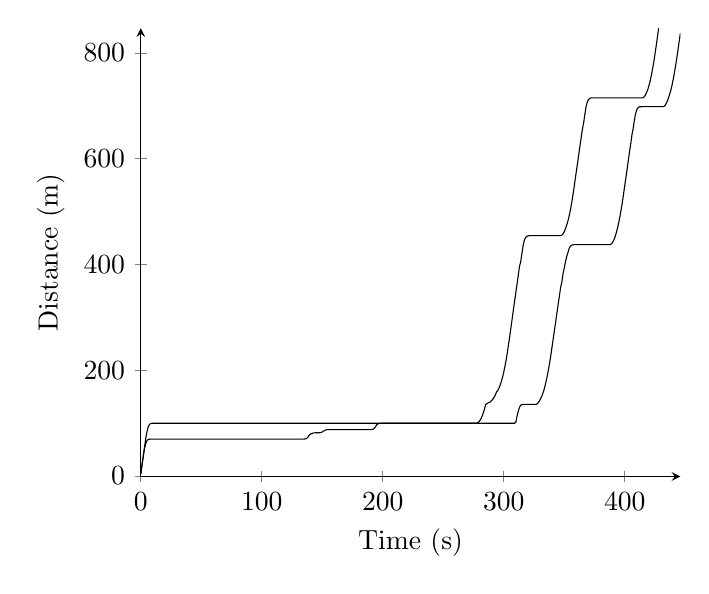
\begin{tikzpicture}
\begin{axis}[
legend style={anchor=west},
axis x line=bottom,
axis y line=left,
ymin=-1,
xlabel=Time (s),
ylabel=Distance (m),
]
\addplot[] coordinates {
(0, 4.1)
(1, 19.9460053715)
(2, 36.2974897012)
(3, 52.7974964837)
(4, 68.8395941663)
(5, 82.2515459976)
(6, 91.8982651099)
(7, 96.7826630145)
(8, 99.0284822845)
(9, 99.624765298)
(10, 99.6992386304)
(11, 99.7103695027)
(12, 99.7103695027)
(13, 99.7103695027)
(14, 99.7103695027)
(15, 99.7103695027)
(16, 99.7103695027)
(17, 99.7103695027)
(18, 99.7103695027)
(19, 99.7103695027)
(20, 99.7103695027)
(21, 99.7103695027)
(22, 99.7103695027)
(23, 99.7103695027)
(24, 99.7103695027)
(25, 99.7103695027)
(26, 99.7103695027)
(27, 99.7103695027)
(28, 99.7103695027)
(29, 99.7103695027)
(30, 99.7103695027)
(31, 99.7103695027)
(32, 99.7103695027)
(33, 99.7103695027)
(34, 99.7103695027)
(35, 99.7103695027)
(36, 99.7103695027)
(37, 99.7103695027)
(38, 99.7103695027)
(39, 99.7103695027)
(40, 99.7103695027)
(41, 99.7103695027)
(42, 99.7103695027)
(43, 99.7103695027)
(44, 99.7103695027)
(45, 99.7103695027)
(46, 99.7103695027)
(47, 99.7103695027)
(48, 99.7103695027)
(49, 99.7103695027)
(50, 99.7103695027)
(51, 99.7103695027)
(52, 99.7103695027)
(53, 99.7103695027)
(54, 99.7103695027)
(55, 99.7103695027)
(56, 99.7103695027)
(57, 99.7103695027)
(58, 99.7103695027)
(59, 99.7103695027)
(60, 99.7103695027)
(61, 99.7103695027)
(62, 99.7103695027)
(63, 99.7103695027)
(64, 99.7103695027)
(65, 99.7103695027)
(66, 99.7103695027)
(67, 99.7103695027)
(68, 99.7103695027)
(69, 99.7103695027)
(70, 99.7103695027)
(71, 99.7103695027)
(72, 99.7103695027)
(73, 99.7103695027)
(74, 99.7103695027)
(75, 99.7103695027)
(76, 99.7103695027)
(77, 99.7103695027)
(78, 99.7103695027)
(79, 99.7103695027)
(80, 99.7103695027)
(81, 99.7103695027)
(82, 99.7103695027)
(83, 99.7103695027)
(84, 99.7103695027)
(85, 99.7103695027)
(86, 99.7103695027)
(87, 99.7103695027)
(88, 99.7103695027)
(89, 99.7103695027)
(90, 99.7103695027)
(91, 99.7103695027)
(92, 99.7103695027)
(93, 99.7103695027)
(94, 99.7103695027)
(95, 99.7103695027)
(96, 99.7103695027)
(97, 99.7103695027)
(98, 99.7103695027)
(99, 99.7103695027)
(100, 99.7103695027)
(101, 99.7103695027)
(102, 99.7103695027)
(103, 99.7103695027)
(104, 99.7103695027)
(105, 99.7103695027)
(106, 99.7103695027)
(107, 99.7103695027)
(108, 99.7103695027)
(109, 99.7103695027)
(110, 99.7103695027)
(111, 99.7103695027)
(112, 99.7103695027)
(113, 99.7103695027)
(114, 99.7103695027)
(115, 99.7103695027)
(116, 99.7103695027)
(117, 99.7103695027)
(118, 99.7103695027)
(119, 99.7103695027)
(120, 99.7103695027)
(121, 99.7103695027)
(122, 99.7103695027)
(123, 99.7103695027)
(124, 99.7103695027)
(125, 99.7103695027)
(126, 99.7103695027)
(127, 99.7103695027)
(128, 99.7103695027)
(129, 99.7103695027)
(130, 99.7103695027)
(131, 99.7103695027)
(132, 99.7103695027)
(133, 99.7103695027)
(134, 99.7103695027)
(135, 99.7103695027)
(136, 99.7103695027)
(137, 99.7103695027)
(138, 99.7103695027)
(139, 99.7103695027)
(140, 99.7103695027)
(141, 99.7103695027)
(142, 99.7103695027)
(143, 99.7103695027)
(144, 99.7103695027)
(145, 99.7103695027)
(146, 99.7103695027)
(147, 99.7103695027)
(148, 99.7103695027)
(149, 99.7103695027)
(150, 99.7103695027)
(151, 99.7103695027)
(152, 99.7103695027)
(153, 99.7103695027)
(154, 99.7103695027)
(155, 99.7103695027)
(156, 99.7103695027)
(157, 99.7103695027)
(158, 99.7103695027)
(159, 99.7103695027)
(160, 99.7103695027)
(161, 99.7103695027)
(162, 99.7103695027)
(163, 99.7103695027)
(164, 99.7103695027)
(165, 99.7103695027)
(166, 99.7103695027)
(167, 99.7103695027)
(168, 99.7103695027)
(169, 99.7103695027)
(170, 99.7103695027)
(171, 99.7103695027)
(172, 99.7103695027)
(173, 99.7103695027)
(174, 99.7103695027)
(175, 99.7103695027)
(176, 99.7103695027)
(177, 99.7103695027)
(178, 99.7103695027)
(179, 99.7103695027)
(180, 99.7103695027)
(181, 99.7103695027)
(182, 99.7103695027)
(183, 99.7103695027)
(184, 99.7103695027)
(185, 99.7103695027)
(186, 99.7103695027)
(187, 99.7103695027)
(188, 99.7103695027)
(189, 99.7103695027)
(190, 99.7103695027)
(191, 99.7103695027)
(192, 99.7103695027)
(193, 99.7103695027)
(194, 99.7103695027)
(195, 99.7103695027)
(196, 99.7103695027)
(197, 99.7103695027)
(198, 99.7103695027)
(199, 99.7103695027)
(200, 99.7103695027)
(201, 99.7103695027)
(202, 99.7103695027)
(203, 99.7103695027)
(204, 99.7103695027)
(205, 99.7103695027)
(206, 99.7103695027)
(207, 99.7103695027)
(208, 99.7103695027)
(209, 99.7103695027)
(210, 99.7103695027)
(211, 99.7103695027)
(212, 99.7103695027)
(213, 99.7103695027)
(214, 99.7103695027)
(215, 99.7103695027)
(216, 99.7103695027)
(217, 99.7103695027)
(218, 99.7103695027)
(219, 99.7103695027)
(220, 99.7103695027)
(221, 99.7103695027)
(222, 99.7103695027)
(223, 99.7103695027)
(224, 99.7103695027)
(225, 99.7103695027)
(226, 99.7103695027)
(227, 99.7103695027)
(228, 99.7103695027)
(229, 99.7103695027)
(230, 99.7103695027)
(231, 99.7103695027)
(232, 99.7103695027)
(233, 99.7103695027)
(234, 99.7103695027)
(235, 99.7103695027)
(236, 99.7103695027)
(237, 99.7103695027)
(238, 99.7103695027)
(239, 99.7103695027)
(240, 99.7103695027)
(241, 99.7103695027)
(242, 99.7103695027)
(243, 99.7103695027)
(244, 99.7103695027)
(245, 99.7103695027)
(246, 99.7103695027)
(247, 99.7103695027)
(248, 99.7103695027)
(249, 99.7103695027)
(250, 99.7103695027)
(251, 99.7103695027)
(252, 99.7103695027)
(253, 99.7103695027)
(254, 99.7103695027)
(255, 99.7103695027)
(256, 99.7103695027)
(257, 99.7103695027)
(258, 99.7103695027)
(259, 99.7103695027)
(260, 99.7103695027)
(261, 99.7103695027)
(262, 99.7103695027)
(263, 99.7103695027)
(264, 99.7103695027)
(265, 99.7103695027)
(266, 99.7103695027)
(267, 99.7103695027)
(268, 99.7103695027)
(269, 99.7103695027)
(270, 99.7103695027)
(271, 99.7103695027)
(272, 99.7103695027)
(273, 99.7103695027)
(274, 99.7103695027)
(275, 99.7103695027)
(276, 99.7103695027)
(277, 99.7103695027)
(278, 99.7103695027)
(279, 99.7103695027)
(280, 99.7103695027)
(281, 99.7103695027)
(282, 99.7103695027)
(283, 99.7103695027)
(284, 99.7103695027)
(285, 99.7103695027)
(286, 99.7103695027)
(287, 99.7103695027)
(288, 99.7103695027)
(289, 99.7103695027)
(290, 99.7103695027)
(291, 99.7103695027)
(292, 99.7103695027)
(293, 99.7103695027)
(294, 99.7103695027)
(295, 99.7103695027)
(296, 99.7103695027)
(297, 99.7103695027)
(298, 99.7103695027)
(299, 99.7103695027)
(300, 99.7103695027)
(301, 99.7103695027)
(302, 99.7103695027)
(303, 99.7103695027)
(304, 99.7103695027)
(305, 99.7103695027)
(306, 99.7103695027)
(307, 99.7103695027)
(308, 99.7103695027)
(309, 99.7103695027)
(310, 101.72)
(311, 113.505338954)
(312, 122.615950544)
(313, 129.878103264)
(314, 133.860409904)
(315, 134.908673684)
(316, 135.260758555)
(317, 135.291802473)
(318, 135.307417201)
(319, 135.307417201)
(320, 135.307417201)
(321, 135.307417201)
(322, 135.307417201)
(323, 135.307417201)
(324, 135.307417201)
(325, 135.307417201)
(326, 135.307417201)
(327, 135.727967391)
(328, 137.294367601)
(329, 140.115604148)
(330, 143.930287049)
(331, 148.538716586)
(332, 154.107897325)
(333, 160.945214813)
(334, 169.302550323)
(335, 179.009820817)
(336, 189.765721678)
(337, 201.692986638)
(338, 215.083363455)
(339, 229.701692131)
(340, 245.867138424)
(341, 261.509121547)
(342, 277.416525077)
(343, 292.830598547)
(344, 309.351103846)
(345, 325.137565322)
(346, 340.807232496)
(347, 356.52758996)
(348, 366.660380233)
(349, 382.386888732)
(350, 393.383293517)
(351, 404.537846077)
(352, 414.762461324)
(353, 421.954031677)
(354, 429.985995135)
(355, 434.273645897)
(356, 436.119960601)
(357, 436.800602752)
(358, 437.272249589)
(359, 437.346705315)
(360, 437.346705315)
(361, 437.346705315)
(362, 437.346705315)
(363, 437.346705315)
(364, 437.346705315)
(365, 437.346705315)
(366, 437.346705315)
(367, 437.346705315)
(368, 437.346705315)
(369, 437.346705315)
(370, 437.346705315)
(371, 437.346705315)
(372, 437.346705315)
(373, 437.346705315)
(374, 437.346705315)
(375, 437.346705315)
(376, 437.346705315)
(377, 437.346705315)
(378, 437.346705315)
(379, 437.346705315)
(380, 437.346705315)
(381, 437.346705315)
(382, 437.346705315)
(383, 437.346705315)
(384, 437.346705315)
(385, 437.346705315)
(386, 437.346705315)
(387, 437.346705315)
(388, 437.346705315)
(389, 439.076116364)
(390, 441.777682558)
(391, 446.21176972)
(392, 452.150943526)
(393, 459.767264483)
(394, 468.721582583)
(395, 478.755909577)
(396, 490.324739668)
(397, 503.046309275)
(398, 517.209367313)
(399, 533.071804743)
(400, 549.128398971)
(401, 564.956774411)
(402, 581.090888314)
(403, 597.645706605)
(404, 613.685703018)
(405, 629.444804561)
(406, 645.705755135)
(407, 657.444264897)
(408, 673.325452169)
(409, 685.252741321)
(410, 692.803289465)
(411, 696.06711972)
(412, 697.855012521)
(413, 698.046096188)
(414, 698.106654143)
(415, 698.134525634)
(416, 698.146918541)
(417, 698.146918541)
(418, 698.146918541)
(419, 698.146918541)
(420, 698.146918541)
(421, 698.146918541)
(422, 698.146918541)
(423, 698.146918541)
(424, 698.146918541)
(425, 698.146918541)
(426, 698.146918541)
(427, 698.146918541)
(428, 698.146918541)
(429, 698.146918541)
(430, 698.146918541)
(431, 698.146918541)
(432, 698.146918541)
(433, 699.659485562)
(434, 702.889240245)
(435, 707.688773008)
(436, 713.707747868)
(437, 720.645618326)
(438, 728.57153771)
(439, 738.101220121)
(440, 749.171739533)
(441, 761.698957182)
(442, 775.186610215)
(443, 790.161961057)
(444, 805.924940118)
(445, 821.647955058)
(446, 837.647240095)
};
\addplot[] coordinates {
(0, 4.1)
(1, 20.5063530304)
(2, 36.5749601919)
(3, 50.7796055157)
(4, 60.5931506146)
(5, 66.4437989106)
(6, 68.8152376735)
(7, 69.5249823374)
(8, 69.6158943966)
(9, 69.664472823)
(10, 69.6862215893)
(11, 69.6862215893)
(12, 69.6862215893)
(13, 69.6862215893)
(14, 69.6862215893)
(15, 69.6862215893)
(16, 69.6862215893)
(17, 69.6862215893)
(18, 69.6862215893)
(19, 69.6862215893)
(20, 69.6862215893)
(21, 69.6862215893)
(22, 69.6862215893)
(23, 69.6862215893)
(24, 69.6862215893)
(25, 69.6862215893)
(26, 69.6862215893)
(27, 69.6862215893)
(28, 69.6862215893)
(29, 69.6862215893)
(30, 69.6862215893)
(31, 69.6862215893)
(32, 69.6862215893)
(33, 69.6862215893)
(34, 69.6862215893)
(35, 69.6862215893)
(36, 69.6862215893)
(37, 69.6862215893)
(38, 69.6862215893)
(39, 69.6862215893)
(40, 69.6862215893)
(41, 69.6862215893)
(42, 69.6862215893)
(43, 69.6862215893)
(44, 69.6862215893)
(45, 69.6862215893)
(46, 69.6862215893)
(47, 69.6862215893)
(48, 69.6862215893)
(49, 69.6862215893)
(50, 69.6862215893)
(51, 69.6862215893)
(52, 69.6862215893)
(53, 69.6862215893)
(54, 69.6862215893)
(55, 69.6862215893)
(56, 69.6862215893)
(57, 69.6862215893)
(58, 69.6862215893)
(59, 69.6862215893)
(60, 69.6862215893)
(61, 69.6862215893)
(62, 69.6862215893)
(63, 69.6862215893)
(64, 69.6862215893)
(65, 69.6862215893)
(66, 69.6862215893)
(67, 69.6862215893)
(68, 69.6862215893)
(69, 69.6862215893)
(70, 69.6862215893)
(71, 69.6862215893)
(72, 69.6862215893)
(73, 69.6862215893)
(74, 69.6862215893)
(75, 69.6862215893)
(76, 69.6862215893)
(77, 69.6862215893)
(78, 69.6862215893)
(79, 69.6862215893)
(80, 69.6862215893)
(81, 69.6862215893)
(82, 69.6862215893)
(83, 69.6862215893)
(84, 69.6862215893)
(85, 69.6862215893)
(86, 69.6862215893)
(87, 69.6862215893)
(88, 69.6862215893)
(89, 69.6862215893)
(90, 69.6862215893)
(91, 69.6862215893)
(92, 69.6862215893)
(93, 69.6862215893)
(94, 69.6862215893)
(95, 69.6862215893)
(96, 69.6862215893)
(97, 69.6862215893)
(98, 69.6862215893)
(99, 69.6862215893)
(100, 69.6862215893)
(101, 69.6862215893)
(102, 69.6862215893)
(103, 69.6862215893)
(104, 69.6862215893)
(105, 69.6862215893)
(106, 69.6862215893)
(107, 69.6862215893)
(108, 69.6862215893)
(109, 69.6862215893)
(110, 69.6862215893)
(111, 69.6862215893)
(112, 69.6862215893)
(113, 69.6862215893)
(114, 69.6862215893)
(115, 69.6862215893)
(116, 69.6862215893)
(117, 69.6862215893)
(118, 69.6862215893)
(119, 69.6862215893)
(120, 69.6862215893)
(121, 69.6862215893)
(122, 69.6862215893)
(123, 69.6862215893)
(124, 69.6862215893)
(125, 69.6862215893)
(126, 69.6862215893)
(127, 69.6862215893)
(128, 69.6862215893)
(129, 69.6862215893)
(130, 69.6862215893)
(131, 69.6862215893)
(132, 69.6862215893)
(133, 69.6862215893)
(134, 69.6862215893)
(135, 69.8875699445)
(136, 70.2130646404)
(137, 70.8567206814)
(138, 73.2247341218)
(139, 76.2974192174)
(140, 78.8083914678)
(141, 80.1024406552)
(142, 80.81535175)
(143, 81.5978032256)
(144, 81.6577658808)
(145, 81.7116096957)
(146, 81.7116096957)
(147, 81.7116096957)
(148, 81.7116096957)
(149, 82.2714449861)
(150, 83.2678965428)
(151, 85.0522073805)
(152, 86.1129863637)
(153, 87.1939461993)
(154, 87.576401671)
(155, 87.6918317117)
(156, 87.7070927823)
(157, 87.7070927823)
(158, 87.7070927823)
(159, 87.7070927823)
(160, 87.7070927823)
(161, 87.7070927823)
(162, 87.7070927823)
(163, 87.7070927823)
(164, 87.7070927823)
(165, 87.7070927823)
(166, 87.7070927823)
(167, 87.7070927823)
(168, 87.7070927823)
(169, 87.7070927823)
(170, 87.7070927823)
(171, 87.7070927823)
(172, 87.7070927823)
(173, 87.7070927823)
(174, 87.7070927823)
(175, 87.7070927823)
(176, 87.7070927823)
(177, 87.7070927823)
(178, 87.7070927823)
(179, 87.7070927823)
(180, 87.7070927823)
(181, 87.7070927823)
(182, 87.7070927823)
(183, 87.7070927823)
(184, 87.7070927823)
(185, 87.7070927823)
(186, 87.7070927823)
(187, 87.7070927823)
(188, 87.7070927823)
(189, 87.7070927823)
(190, 87.7070927823)
(191, 87.7070927823)
(192, 88.5214530367)
(193, 90.3659884509)
(194, 92.9629932577)
(195, 96.8750784434)
(196, 98.6260081417)
(197, 99.2422110886)
(198, 99.5415169609)
(199, 99.6939916291)
(200, 99.7154901814)
(201, 99.7154901814)
(202, 99.7154901814)
(203, 99.7154901814)
(204, 99.7154901814)
(205, 99.7154901814)
(206, 99.7154901814)
(207, 99.7154901814)
(208, 99.7154901814)
(209, 99.7154901814)
(210, 99.7154901814)
(211, 99.7154901814)
(212, 99.7154901814)
(213, 99.7154901814)
(214, 99.7154901814)
(215, 99.7154901814)
(216, 99.7154901814)
(217, 99.7154901814)
(218, 99.7154901814)
(219, 99.7154901814)
(220, 99.7154901814)
(221, 99.7154901814)
(222, 99.7154901814)
(223, 99.7154901814)
(224, 99.7154901814)
(225, 99.7154901814)
(226, 99.7154901814)
(227, 99.7154901814)
(228, 99.7154901814)
(229, 99.7154901814)
(230, 99.7154901814)
(231, 99.7154901814)
(232, 99.7154901814)
(233, 99.7154901814)
(234, 99.7154901814)
(235, 99.7154901814)
(236, 99.7154901814)
(237, 99.7154901814)
(238, 99.7154901814)
(239, 99.7154901814)
(240, 99.7154901814)
(241, 99.7154901814)
(242, 99.7154901814)
(243, 99.7154901814)
(244, 99.7154901814)
(245, 99.7154901814)
(246, 99.7154901814)
(247, 99.7154901814)
(248, 99.7154901814)
(249, 99.7154901814)
(250, 99.7154901814)
(251, 99.7154901814)
(252, 99.7154901814)
(253, 99.7154901814)
(254, 99.7154901814)
(255, 99.7154901814)
(256, 99.7154901814)
(257, 99.7154901814)
(258, 99.7154901814)
(259, 99.7154901814)
(260, 99.7154901814)
(261, 99.7154901814)
(262, 99.7154901814)
(263, 99.7154901814)
(264, 99.7154901814)
(265, 99.7154901814)
(266, 99.7154901814)
(267, 99.7154901814)
(268, 99.7154901814)
(269, 99.7154901814)
(270, 99.7154901814)
(271, 99.7154901814)
(272, 99.7154901814)
(273, 99.7154901814)
(274, 99.7154901814)
(275, 99.7154901814)
(276, 99.7154901814)
(277, 99.7154901814)
(278, 99.7154901814)
(279, 101.33594632)
(280, 104.002898881)
(281, 107.76679922)
(282, 112.472555161)
(283, 118.764115626)
(284, 126.128410527)
(285, 134.948665929)
(286, 136.400390193)
(287, 138.203758421)
(288, 138.990570492)
(289, 140.520893557)
(290, 142.908340031)
(291, 145.313292909)
(292, 148.6307092)
(293, 152.934753759)
(294, 158.681600324)
(295, 161.525433858)
(296, 166.033345417)
(297, 171.628954889)
(298, 178.687459191)
(299, 186.709680162)
(300, 196.476476118)
(301, 207.651029862)
(302, 219.977783026)
(303, 233.840168973)
(304, 249.38689278)
(305, 265.115371155)
(306, 281.642977076)
(307, 298.227015074)
(308, 314.815764436)
(309, 331.160383456)
(310, 347.290845268)
(311, 363.282551582)
(312, 379.793181586)
(313, 396.251401857)
(314, 404.868859653)
(315, 420.719574545)
(316, 435.586340538)
(317, 445.588113468)
(318, 450.885502329)
(319, 452.850321597)
(320, 453.880347034)
(321, 454.245788674)
(322, 454.256147814)
(323, 454.256147814)
(324, 454.256147814)
(325, 454.256147814)
(326, 454.256147814)
(327, 454.256147814)
(328, 454.256147814)
(329, 454.256147814)
(330, 454.256147814)
(331, 454.256147814)
(332, 454.256147814)
(333, 454.256147814)
(334, 454.256147814)
(335, 454.256147814)
(336, 454.256147814)
(337, 454.256147814)
(338, 454.256147814)
(339, 454.256147814)
(340, 454.256147814)
(341, 454.256147814)
(342, 454.256147814)
(343, 454.256147814)
(344, 454.256147814)
(345, 454.256147814)
(346, 454.256147814)
(347, 454.256147814)
(348, 455.431924543)
(349, 457.779987223)
(350, 461.659239929)
(351, 467.24997766)
(352, 474.086975845)
(353, 481.83004873)
(354, 491.12238531)
(355, 502.029074389)
(356, 514.44151056)
(357, 528.504260247)
(358, 543.728389396)
(359, 560.152502112)
(360, 575.926326338)
(361, 591.928991271)
(362, 608.129595027)
(363, 624.149298752)
(364, 639.956117163)
(365, 655.912963345)
(366, 667.266786824)
(367, 683.441159313)
(368, 697.562306268)
(369, 706.492754755)
(370, 711.549931225)
(371, 713.759192483)
(372, 714.498129643)
(373, 714.835732095)
(374, 714.866189775)
(375, 714.876137341)
(376, 714.876137341)
(377, 714.876137341)
(378, 714.876137341)
(379, 714.876137341)
(380, 714.876137341)
(381, 714.876137341)
(382, 714.876137341)
(383, 714.876137341)
(384, 714.876137341)
(385, 714.876137341)
(386, 714.876137341)
(387, 714.876137341)
(388, 714.876137341)
(389, 714.876137341)
(390, 714.876137341)
(391, 714.876137341)
(392, 714.876137341)
(393, 714.876137341)
(394, 714.876137341)
(395, 714.876137341)
(396, 714.876137341)
(397, 714.876137341)
(398, 714.876137341)
(399, 714.876137341)
(400, 714.876137341)
(401, 714.876137341)
(402, 714.876137341)
(403, 714.876137341)
(404, 714.876137341)
(405, 714.876137341)
(406, 714.876137341)
(407, 714.876137341)
(408, 714.876137341)
(409, 714.876137341)
(410, 714.876137341)
(411, 714.876137341)
(412, 714.876137341)
(413, 714.876137341)
(414, 714.876137341)
(415, 714.876137341)
(416, 716.632727423)
(417, 720.012996771)
(418, 724.747590821)
(419, 730.446789079)
(420, 737.941627434)
(421, 746.961274103)
(422, 757.669587502)
(423, 769.654411416)
(424, 782.870989621)
(425, 797.761725603)
(426, 813.505251596)
(427, 829.971426056)
(428, 846.42360993)
};

\end{axis}
\end{tikzpicture}
\label{tik:distance:0:51}
\caption{0 percent diving with GSC on route $51$}
\end{figure}

%
\begin{figure}
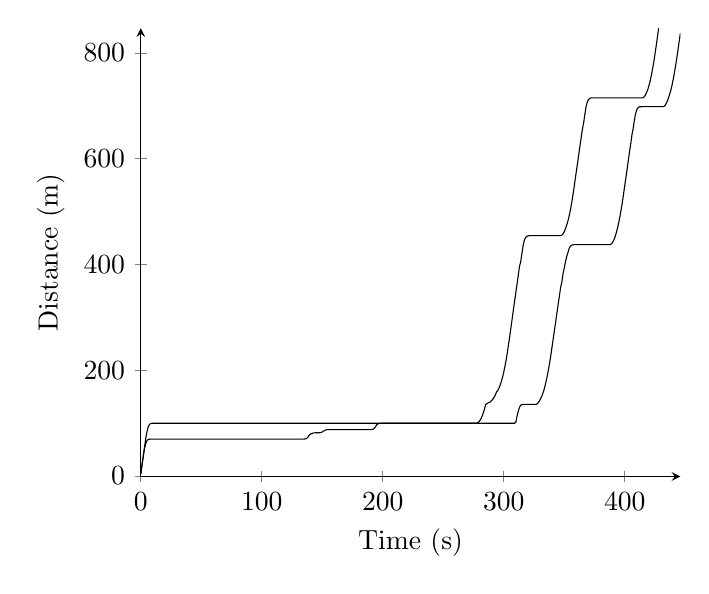
\begin{tikzpicture}
\begin{axis}[
legend style={anchor=west},
axis x line=bottom,
axis y line=left,
ymin=-1,
xlabel=Time (s),
ylabel=Distance (m),
]
\addplot[] coordinates {
(0, 4.1)
(1, 19.9460053715)
(2, 36.2974897012)
(3, 52.7974964837)
(4, 68.8395941663)
(5, 82.2515459976)
(6, 91.8982651099)
(7, 96.7826630145)
(8, 99.0284822845)
(9, 99.624765298)
(10, 99.6992386304)
(11, 99.7103695027)
(12, 99.7103695027)
(13, 99.7103695027)
(14, 99.7103695027)
(15, 99.7103695027)
(16, 99.7103695027)
(17, 99.7103695027)
(18, 99.7103695027)
(19, 99.7103695027)
(20, 99.7103695027)
(21, 99.7103695027)
(22, 99.7103695027)
(23, 99.7103695027)
(24, 99.7103695027)
(25, 99.7103695027)
(26, 99.7103695027)
(27, 99.7103695027)
(28, 99.7103695027)
(29, 99.7103695027)
(30, 99.7103695027)
(31, 99.7103695027)
(32, 99.7103695027)
(33, 99.7103695027)
(34, 99.7103695027)
(35, 99.7103695027)
(36, 99.7103695027)
(37, 99.7103695027)
(38, 99.7103695027)
(39, 99.7103695027)
(40, 99.7103695027)
(41, 99.7103695027)
(42, 99.7103695027)
(43, 99.7103695027)
(44, 99.7103695027)
(45, 99.7103695027)
(46, 99.7103695027)
(47, 99.7103695027)
(48, 99.7103695027)
(49, 99.7103695027)
(50, 99.7103695027)
(51, 99.7103695027)
(52, 99.7103695027)
(53, 99.7103695027)
(54, 99.7103695027)
(55, 99.7103695027)
(56, 99.7103695027)
(57, 99.7103695027)
(58, 99.7103695027)
(59, 99.7103695027)
(60, 99.7103695027)
(61, 99.7103695027)
(62, 99.7103695027)
(63, 99.7103695027)
(64, 99.7103695027)
(65, 99.7103695027)
(66, 99.7103695027)
(67, 99.7103695027)
(68, 99.7103695027)
(69, 99.7103695027)
(70, 99.7103695027)
(71, 99.7103695027)
(72, 99.7103695027)
(73, 99.7103695027)
(74, 99.7103695027)
(75, 99.7103695027)
(76, 99.7103695027)
(77, 99.7103695027)
(78, 99.7103695027)
(79, 99.7103695027)
(80, 99.7103695027)
(81, 99.7103695027)
(82, 99.7103695027)
(83, 99.7103695027)
(84, 99.7103695027)
(85, 99.7103695027)
(86, 99.7103695027)
(87, 99.7103695027)
(88, 99.7103695027)
(89, 99.7103695027)
(90, 99.7103695027)
(91, 99.7103695027)
(92, 99.7103695027)
(93, 99.7103695027)
(94, 99.7103695027)
(95, 99.7103695027)
(96, 99.7103695027)
(97, 99.7103695027)
(98, 99.7103695027)
(99, 99.7103695027)
(100, 99.7103695027)
(101, 99.7103695027)
(102, 99.7103695027)
(103, 99.7103695027)
(104, 99.7103695027)
(105, 99.7103695027)
(106, 99.7103695027)
(107, 99.7103695027)
(108, 99.7103695027)
(109, 99.7103695027)
(110, 99.7103695027)
(111, 99.7103695027)
(112, 99.7103695027)
(113, 99.7103695027)
(114, 99.7103695027)
(115, 99.7103695027)
(116, 99.7103695027)
(117, 99.7103695027)
(118, 99.7103695027)
(119, 99.7103695027)
(120, 99.7103695027)
(121, 99.7103695027)
(122, 99.7103695027)
(123, 99.7103695027)
(124, 99.7103695027)
(125, 99.7103695027)
(126, 99.7103695027)
(127, 99.7103695027)
(128, 99.7103695027)
(129, 99.7103695027)
(130, 99.7103695027)
(131, 99.7103695027)
(132, 99.7103695027)
(133, 99.7103695027)
(134, 99.7103695027)
(135, 99.7103695027)
(136, 99.7103695027)
(137, 99.7103695027)
(138, 99.7103695027)
(139, 99.7103695027)
(140, 99.7103695027)
(141, 99.7103695027)
(142, 99.7103695027)
(143, 99.7103695027)
(144, 99.7103695027)
(145, 99.7103695027)
(146, 99.7103695027)
(147, 99.7103695027)
(148, 99.7103695027)
(149, 99.7103695027)
(150, 99.7103695027)
(151, 99.7103695027)
(152, 99.7103695027)
(153, 99.7103695027)
(154, 99.7103695027)
(155, 99.7103695027)
(156, 99.7103695027)
(157, 99.7103695027)
(158, 99.7103695027)
(159, 99.7103695027)
(160, 99.7103695027)
(161, 99.7103695027)
(162, 99.7103695027)
(163, 99.7103695027)
(164, 99.7103695027)
(165, 99.7103695027)
(166, 99.7103695027)
(167, 99.7103695027)
(168, 99.7103695027)
(169, 99.7103695027)
(170, 99.7103695027)
(171, 99.7103695027)
(172, 99.7103695027)
(173, 99.7103695027)
(174, 99.7103695027)
(175, 99.7103695027)
(176, 99.7103695027)
(177, 99.7103695027)
(178, 99.7103695027)
(179, 99.7103695027)
(180, 99.7103695027)
(181, 99.7103695027)
(182, 99.7103695027)
(183, 99.7103695027)
(184, 99.7103695027)
(185, 99.7103695027)
(186, 99.7103695027)
(187, 99.7103695027)
(188, 99.7103695027)
(189, 99.7103695027)
(190, 99.7103695027)
(191, 99.7103695027)
(192, 99.7103695027)
(193, 99.7103695027)
(194, 99.7103695027)
(195, 99.7103695027)
(196, 99.7103695027)
(197, 99.7103695027)
(198, 99.7103695027)
(199, 99.7103695027)
(200, 99.7103695027)
(201, 99.7103695027)
(202, 99.7103695027)
(203, 99.7103695027)
(204, 99.7103695027)
(205, 99.7103695027)
(206, 99.7103695027)
(207, 99.7103695027)
(208, 99.7103695027)
(209, 99.7103695027)
(210, 99.7103695027)
(211, 99.7103695027)
(212, 99.7103695027)
(213, 99.7103695027)
(214, 99.7103695027)
(215, 99.7103695027)
(216, 99.7103695027)
(217, 99.7103695027)
(218, 99.7103695027)
(219, 99.7103695027)
(220, 99.7103695027)
(221, 99.7103695027)
(222, 99.7103695027)
(223, 99.7103695027)
(224, 99.7103695027)
(225, 99.7103695027)
(226, 99.7103695027)
(227, 99.7103695027)
(228, 99.7103695027)
(229, 99.7103695027)
(230, 99.7103695027)
(231, 99.7103695027)
(232, 99.7103695027)
(233, 99.7103695027)
(234, 99.7103695027)
(235, 99.7103695027)
(236, 99.7103695027)
(237, 99.7103695027)
(238, 99.7103695027)
(239, 99.7103695027)
(240, 99.7103695027)
(241, 99.7103695027)
(242, 99.7103695027)
(243, 99.7103695027)
(244, 99.7103695027)
(245, 99.7103695027)
(246, 99.7103695027)
(247, 99.7103695027)
(248, 99.7103695027)
(249, 99.7103695027)
(250, 99.7103695027)
(251, 99.7103695027)
(252, 99.7103695027)
(253, 99.7103695027)
(254, 99.7103695027)
(255, 99.7103695027)
(256, 99.7103695027)
(257, 99.7103695027)
(258, 99.7103695027)
(259, 99.7103695027)
(260, 99.7103695027)
(261, 99.7103695027)
(262, 99.7103695027)
(263, 99.7103695027)
(264, 99.7103695027)
(265, 99.7103695027)
(266, 99.7103695027)
(267, 99.7103695027)
(268, 99.7103695027)
(269, 99.7103695027)
(270, 99.7103695027)
(271, 99.7103695027)
(272, 99.7103695027)
(273, 99.7103695027)
(274, 99.7103695027)
(275, 99.7103695027)
(276, 99.7103695027)
(277, 99.7103695027)
(278, 99.7103695027)
(279, 99.7103695027)
(280, 99.7103695027)
(281, 99.7103695027)
(282, 99.7103695027)
(283, 99.7103695027)
(284, 99.7103695027)
(285, 99.7103695027)
(286, 99.7103695027)
(287, 99.7103695027)
(288, 99.7103695027)
(289, 99.7103695027)
(290, 99.7103695027)
(291, 99.7103695027)
(292, 99.7103695027)
(293, 99.7103695027)
(294, 99.7103695027)
(295, 99.7103695027)
(296, 99.7103695027)
(297, 99.7103695027)
(298, 99.7103695027)
(299, 99.7103695027)
(300, 99.7103695027)
(301, 99.7103695027)
(302, 99.7103695027)
(303, 99.7103695027)
(304, 99.7103695027)
(305, 99.7103695027)
(306, 99.7103695027)
(307, 99.7103695027)
(308, 99.7103695027)
(309, 99.7103695027)
(310, 101.72)
(311, 113.505338954)
(312, 122.615950544)
(313, 129.878103264)
(314, 133.860409904)
(315, 134.908673684)
(316, 135.260758555)
(317, 135.291802473)
(318, 135.307417201)
(319, 135.307417201)
(320, 135.307417201)
(321, 135.307417201)
(322, 135.307417201)
(323, 135.307417201)
(324, 135.307417201)
(325, 135.307417201)
(326, 135.307417201)
(327, 135.727967391)
(328, 137.294367601)
(329, 140.115604148)
(330, 143.930287049)
(331, 148.538716586)
(332, 154.107897325)
(333, 160.945214813)
(334, 169.302550323)
(335, 179.009820817)
(336, 189.765721678)
(337, 201.692986638)
(338, 215.083363455)
(339, 229.701692131)
(340, 245.867138424)
(341, 261.509121547)
(342, 277.416525077)
(343, 292.830598547)
(344, 309.351103846)
(345, 325.137565322)
(346, 340.807232496)
(347, 356.52758996)
(348, 366.660380233)
(349, 382.386888732)
(350, 393.383293517)
(351, 404.537846077)
(352, 414.762461324)
(353, 421.954031677)
(354, 429.985995135)
(355, 434.273645897)
(356, 436.119960601)
(357, 436.800602752)
(358, 437.272249589)
(359, 437.346705315)
(360, 437.346705315)
(361, 437.346705315)
(362, 437.346705315)
(363, 437.346705315)
(364, 437.346705315)
(365, 437.346705315)
(366, 437.346705315)
(367, 437.346705315)
(368, 437.346705315)
(369, 437.346705315)
(370, 437.346705315)
(371, 437.346705315)
(372, 437.346705315)
(373, 437.346705315)
(374, 437.346705315)
(375, 437.346705315)
(376, 437.346705315)
(377, 437.346705315)
(378, 437.346705315)
(379, 437.346705315)
(380, 437.346705315)
(381, 437.346705315)
(382, 437.346705315)
(383, 437.346705315)
(384, 437.346705315)
(385, 437.346705315)
(386, 437.346705315)
(387, 437.346705315)
(388, 437.346705315)
(389, 439.076116364)
(390, 441.777682558)
(391, 446.21176972)
(392, 452.150943526)
(393, 459.767264483)
(394, 468.721582583)
(395, 478.755909577)
(396, 490.324739668)
(397, 503.046309275)
(398, 517.209367313)
(399, 533.071804743)
(400, 549.128398971)
(401, 564.956774411)
(402, 581.090888314)
(403, 597.645706605)
(404, 613.685703018)
(405, 629.444804561)
(406, 645.705755135)
(407, 657.444264897)
(408, 673.325452169)
(409, 685.252741321)
(410, 692.803289465)
(411, 696.06711972)
(412, 697.855012521)
(413, 698.046096188)
(414, 698.106654143)
(415, 698.134525634)
(416, 698.146918541)
(417, 698.146918541)
(418, 698.146918541)
(419, 698.146918541)
(420, 698.146918541)
(421, 698.146918541)
(422, 698.146918541)
(423, 698.146918541)
(424, 698.146918541)
(425, 698.146918541)
(426, 698.146918541)
(427, 698.146918541)
(428, 698.146918541)
(429, 698.146918541)
(430, 698.146918541)
(431, 698.146918541)
(432, 698.146918541)
(433, 699.659485562)
(434, 702.889240245)
(435, 707.688773008)
(436, 713.707747868)
(437, 720.645618326)
(438, 728.57153771)
(439, 738.101220121)
(440, 749.171739533)
(441, 761.698957182)
(442, 775.186610215)
(443, 790.161961057)
(444, 805.924940118)
(445, 821.647955058)
(446, 837.647240095)
};
\addplot[] coordinates {
(0, 4.1)
(1, 20.5063530304)
(2, 36.5749601919)
(3, 50.7796055157)
(4, 60.5931506146)
(5, 66.4437989106)
(6, 68.8152376735)
(7, 69.5249823374)
(8, 69.6158943966)
(9, 69.664472823)
(10, 69.6862215893)
(11, 69.6862215893)
(12, 69.6862215893)
(13, 69.6862215893)
(14, 69.6862215893)
(15, 69.6862215893)
(16, 69.6862215893)
(17, 69.6862215893)
(18, 69.6862215893)
(19, 69.6862215893)
(20, 69.6862215893)
(21, 69.6862215893)
(22, 69.6862215893)
(23, 69.6862215893)
(24, 69.6862215893)
(25, 69.6862215893)
(26, 69.6862215893)
(27, 69.6862215893)
(28, 69.6862215893)
(29, 69.6862215893)
(30, 69.6862215893)
(31, 69.6862215893)
(32, 69.6862215893)
(33, 69.6862215893)
(34, 69.6862215893)
(35, 69.6862215893)
(36, 69.6862215893)
(37, 69.6862215893)
(38, 69.6862215893)
(39, 69.6862215893)
(40, 69.6862215893)
(41, 69.6862215893)
(42, 69.6862215893)
(43, 69.6862215893)
(44, 69.6862215893)
(45, 69.6862215893)
(46, 69.6862215893)
(47, 69.6862215893)
(48, 69.6862215893)
(49, 69.6862215893)
(50, 69.6862215893)
(51, 69.6862215893)
(52, 69.6862215893)
(53, 69.6862215893)
(54, 69.6862215893)
(55, 69.6862215893)
(56, 69.6862215893)
(57, 69.6862215893)
(58, 69.6862215893)
(59, 69.6862215893)
(60, 69.6862215893)
(61, 69.6862215893)
(62, 69.6862215893)
(63, 69.6862215893)
(64, 69.6862215893)
(65, 69.6862215893)
(66, 69.6862215893)
(67, 69.6862215893)
(68, 69.6862215893)
(69, 69.6862215893)
(70, 69.6862215893)
(71, 69.6862215893)
(72, 69.6862215893)
(73, 69.6862215893)
(74, 69.6862215893)
(75, 69.6862215893)
(76, 69.6862215893)
(77, 69.6862215893)
(78, 69.6862215893)
(79, 69.6862215893)
(80, 69.6862215893)
(81, 69.6862215893)
(82, 69.6862215893)
(83, 69.6862215893)
(84, 69.6862215893)
(85, 69.6862215893)
(86, 69.6862215893)
(87, 69.6862215893)
(88, 69.6862215893)
(89, 69.6862215893)
(90, 69.6862215893)
(91, 69.6862215893)
(92, 69.6862215893)
(93, 69.6862215893)
(94, 69.6862215893)
(95, 69.6862215893)
(96, 69.6862215893)
(97, 69.6862215893)
(98, 69.6862215893)
(99, 69.6862215893)
(100, 69.6862215893)
(101, 69.6862215893)
(102, 69.6862215893)
(103, 69.6862215893)
(104, 69.6862215893)
(105, 69.6862215893)
(106, 69.6862215893)
(107, 69.6862215893)
(108, 69.6862215893)
(109, 69.6862215893)
(110, 69.6862215893)
(111, 69.6862215893)
(112, 69.6862215893)
(113, 69.6862215893)
(114, 69.6862215893)
(115, 69.6862215893)
(116, 69.6862215893)
(117, 69.6862215893)
(118, 69.6862215893)
(119, 69.6862215893)
(120, 69.6862215893)
(121, 69.6862215893)
(122, 69.6862215893)
(123, 69.6862215893)
(124, 69.6862215893)
(125, 69.6862215893)
(126, 69.6862215893)
(127, 69.6862215893)
(128, 69.6862215893)
(129, 69.6862215893)
(130, 69.6862215893)
(131, 69.6862215893)
(132, 69.6862215893)
(133, 69.6862215893)
(134, 69.6862215893)
(135, 69.8875699445)
(136, 70.2130646404)
(137, 70.8567206814)
(138, 73.2247341218)
(139, 76.2974192174)
(140, 78.8083914678)
(141, 80.1024406552)
(142, 80.81535175)
(143, 81.5978032256)
(144, 81.6577658808)
(145, 81.7116096957)
(146, 81.7116096957)
(147, 81.7116096957)
(148, 81.7116096957)
(149, 82.2714449861)
(150, 83.2678965428)
(151, 85.0522073805)
(152, 86.1129863637)
(153, 87.1939461993)
(154, 87.576401671)
(155, 87.6918317117)
(156, 87.7070927823)
(157, 87.7070927823)
(158, 87.7070927823)
(159, 87.7070927823)
(160, 87.7070927823)
(161, 87.7070927823)
(162, 87.7070927823)
(163, 87.7070927823)
(164, 87.7070927823)
(165, 87.7070927823)
(166, 87.7070927823)
(167, 87.7070927823)
(168, 87.7070927823)
(169, 87.7070927823)
(170, 87.7070927823)
(171, 87.7070927823)
(172, 87.7070927823)
(173, 87.7070927823)
(174, 87.7070927823)
(175, 87.7070927823)
(176, 87.7070927823)
(177, 87.7070927823)
(178, 87.7070927823)
(179, 87.7070927823)
(180, 87.7070927823)
(181, 87.7070927823)
(182, 87.7070927823)
(183, 87.7070927823)
(184, 87.7070927823)
(185, 87.7070927823)
(186, 87.7070927823)
(187, 87.7070927823)
(188, 87.7070927823)
(189, 87.7070927823)
(190, 87.7070927823)
(191, 87.7070927823)
(192, 88.5214530367)
(193, 90.3659884509)
(194, 92.9629932577)
(195, 96.8750784434)
(196, 98.6260081417)
(197, 99.2422110886)
(198, 99.5415169609)
(199, 99.6939916291)
(200, 99.7154901814)
(201, 99.7154901814)
(202, 99.7154901814)
(203, 99.7154901814)
(204, 99.7154901814)
(205, 99.7154901814)
(206, 99.7154901814)
(207, 99.7154901814)
(208, 99.7154901814)
(209, 99.7154901814)
(210, 99.7154901814)
(211, 99.7154901814)
(212, 99.7154901814)
(213, 99.7154901814)
(214, 99.7154901814)
(215, 99.7154901814)
(216, 99.7154901814)
(217, 99.7154901814)
(218, 99.7154901814)
(219, 99.7154901814)
(220, 99.7154901814)
(221, 99.7154901814)
(222, 99.7154901814)
(223, 99.7154901814)
(224, 99.7154901814)
(225, 99.7154901814)
(226, 99.7154901814)
(227, 99.7154901814)
(228, 99.7154901814)
(229, 99.7154901814)
(230, 99.7154901814)
(231, 99.7154901814)
(232, 99.7154901814)
(233, 99.7154901814)
(234, 99.7154901814)
(235, 99.7154901814)
(236, 99.7154901814)
(237, 99.7154901814)
(238, 99.7154901814)
(239, 99.7154901814)
(240, 99.7154901814)
(241, 99.7154901814)
(242, 99.7154901814)
(243, 99.7154901814)
(244, 99.7154901814)
(245, 99.7154901814)
(246, 99.7154901814)
(247, 99.7154901814)
(248, 99.7154901814)
(249, 99.7154901814)
(250, 99.7154901814)
(251, 99.7154901814)
(252, 99.7154901814)
(253, 99.7154901814)
(254, 99.7154901814)
(255, 99.7154901814)
(256, 99.7154901814)
(257, 99.7154901814)
(258, 99.7154901814)
(259, 99.7154901814)
(260, 99.7154901814)
(261, 99.7154901814)
(262, 99.7154901814)
(263, 99.7154901814)
(264, 99.7154901814)
(265, 99.7154901814)
(266, 99.7154901814)
(267, 99.7154901814)
(268, 99.7154901814)
(269, 99.7154901814)
(270, 99.7154901814)
(271, 99.7154901814)
(272, 99.7154901814)
(273, 99.7154901814)
(274, 99.7154901814)
(275, 99.7154901814)
(276, 99.7154901814)
(277, 99.7154901814)
(278, 99.7154901814)
(279, 101.33594632)
(280, 104.002898881)
(281, 107.76679922)
(282, 112.472555161)
(283, 118.764115626)
(284, 126.128410527)
(285, 134.948665929)
(286, 136.400390193)
(287, 138.203758421)
(288, 138.990570492)
(289, 140.520893557)
(290, 142.908340031)
(291, 145.313292909)
(292, 148.6307092)
(293, 152.934753759)
(294, 158.681600324)
(295, 161.525433858)
(296, 166.033345417)
(297, 171.628954889)
(298, 178.687459191)
(299, 186.709680162)
(300, 196.476476118)
(301, 207.651029862)
(302, 219.977783026)
(303, 233.840168973)
(304, 249.38689278)
(305, 265.115371155)
(306, 281.642977076)
(307, 298.227015074)
(308, 314.815764436)
(309, 331.160383456)
(310, 347.290845268)
(311, 363.282551582)
(312, 379.793181586)
(313, 396.251401857)
(314, 404.868859653)
(315, 420.719574545)
(316, 435.586340538)
(317, 445.588113468)
(318, 450.885502329)
(319, 452.850321597)
(320, 453.880347034)
(321, 454.245788674)
(322, 454.256147814)
(323, 454.256147814)
(324, 454.256147814)
(325, 454.256147814)
(326, 454.256147814)
(327, 454.256147814)
(328, 454.256147814)
(329, 454.256147814)
(330, 454.256147814)
(331, 454.256147814)
(332, 454.256147814)
(333, 454.256147814)
(334, 454.256147814)
(335, 454.256147814)
(336, 454.256147814)
(337, 454.256147814)
(338, 454.256147814)
(339, 454.256147814)
(340, 454.256147814)
(341, 454.256147814)
(342, 454.256147814)
(343, 454.256147814)
(344, 454.256147814)
(345, 454.256147814)
(346, 454.256147814)
(347, 454.256147814)
(348, 455.431924543)
(349, 457.779987223)
(350, 461.659239929)
(351, 467.24997766)
(352, 474.086975845)
(353, 481.83004873)
(354, 491.12238531)
(355, 502.029074389)
(356, 514.44151056)
(357, 528.504260247)
(358, 543.728389396)
(359, 560.152502112)
(360, 575.926326338)
(361, 591.928991271)
(362, 608.129595027)
(363, 624.149298752)
(364, 639.956117163)
(365, 655.912963345)
(366, 667.266786824)
(367, 683.441159313)
(368, 697.562306268)
(369, 706.492754755)
(370, 711.549931225)
(371, 713.759192483)
(372, 714.498129643)
(373, 714.835732095)
(374, 714.866189775)
(375, 714.876137341)
(376, 714.876137341)
(377, 714.876137341)
(378, 714.876137341)
(379, 714.876137341)
(380, 714.876137341)
(381, 714.876137341)
(382, 714.876137341)
(383, 714.876137341)
(384, 714.876137341)
(385, 714.876137341)
(386, 714.876137341)
(387, 714.876137341)
(388, 714.876137341)
(389, 714.876137341)
(390, 714.876137341)
(391, 714.876137341)
(392, 714.876137341)
(393, 714.876137341)
(394, 714.876137341)
(395, 714.876137341)
(396, 714.876137341)
(397, 714.876137341)
(398, 714.876137341)
(399, 714.876137341)
(400, 714.876137341)
(401, 714.876137341)
(402, 714.876137341)
(403, 714.876137341)
(404, 714.876137341)
(405, 714.876137341)
(406, 714.876137341)
(407, 714.876137341)
(408, 714.876137341)
(409, 714.876137341)
(410, 714.876137341)
(411, 714.876137341)
(412, 714.876137341)
(413, 714.876137341)
(414, 714.876137341)
(415, 714.876137341)
(416, 716.632727423)
(417, 720.012996771)
(418, 724.747590821)
(419, 730.446789079)
(420, 737.941627434)
(421, 746.961274103)
(422, 757.669587502)
(423, 769.654411416)
(424, 782.870989621)
(425, 797.761725603)
(426, 813.505251596)
(427, 829.971426056)
(428, 846.42360993)
};

\end{axis}
\end{tikzpicture}
\label{tik:distance:0:51}
\caption{0 percent diving with GSC on route $51$}
\end{figure}


\subsection{Speed}
Figure~\ref{tik:speed:0:51} shows the speed at which SUMO controlled vehicles on route 51 drive as a function over time.
The graph clearly shows that the vehicles quicly accelerates up to the maximal speed, then quickly decelerates to a full stop and then quickly accelerates again.
By using \tech we see a very different outline (See Figure~\ref{tik:speed:100:51}).
Few vehicles decelerates to $0 m/s$, and many stay above $5 m/s$ ($18 km/h$ or $11$ miles per hour ($mph$)).
We do, however, still see a large fluctuation.
%
\begin{figure}
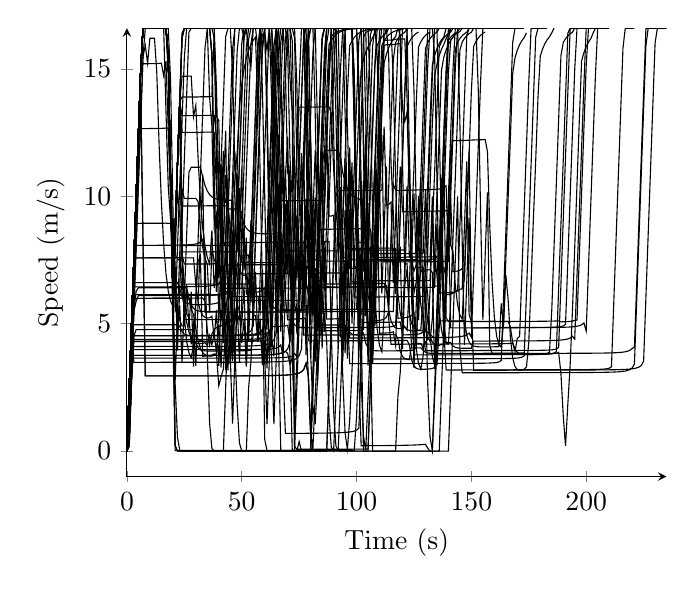
\begin{tikzpicture}
\begin{axis}[
legend style={anchor=west},
axis x line=bottom,
axis y line=left,
ymin=-1,
xlabel=Time (s),
ylabel=Speed (m/s),
]
\addplot[] coordinates {
(0, 0.0)
(1, 1.70108207609)
(2, 4.20108207609)
(3, 6.70108207609)
(4, 9.20108207609)
(5, 11.7010820761)
(6, 14.2010820761)
(7, 8.20108207609)
(8, 2.95038492546)
(9, 2.95041334887)
(10, 2.95044295682)
(11, 2.9504738161)
(12, 2.95050599825)
(13, 2.95053958002)
(14, 2.95057464381)
(15, 2.95061127816)
(16, 2.95064957833)
(17, 2.95068964694)
(18, 2.95073159461)
(19, 2.95077554077)
(20, 2.95082161449)
(21, 2.95086995545)
(22, 2.95092071497)
(23, 2.95097405724)
(24, 2.9510301606)
(25, 2.9510892191)
(26, 2.95115144414)
(27, 2.95121706638)
(28, 2.95128633789)
(29, 2.95135953457)
(30, 2.95143695895)
(31, 2.95151894327)
(32, 2.9516058531)
(33, 2.95169809146)
(34, 2.95179610344)
(35, 2.95190038169)
(36, 2.95201147258)
(37, 2.95212998344)
(38, 2.9522565909)
(39, 2.95239205062)
(40, 2.95253720862)
(41, 2.95269301465)
(42, 2.95286053776)
(43, 2.95304098488)
(44, 2.95323572268)
(45, 2.95344630372)
(46, 2.95367449767)
(47, 2.9539223289)
(48, 2.95419212183)
(49, 2.9544865561)
(50, 2.95480873387)
(51, 2.95516226262)
(52, 2.95555135754)
(53, 2.95598096903)
(54, 2.95645694263)
(55, 2.95698622133)
(56, 2.9575771033)
(57, 2.95823957371)
(58, 2.95898573555)
(59, 2.95983037536)
(60, 2.96079171446)
(61, 2.96189241909)
(62, 2.96316097748)
(63, 2.96463360574)
(64, 2.966801869)
(65, 2.96871538322)
(66, 2.97114643487)
(67, 2.97407974317)
(68, 2.97766601412)
(69, 2.98211811255)
(70, 2.98774528263)
(71, 2.99501216128)
(72, 3.0046461466)
(73, 3.0178462482)
(74, 3.03672593505)
(75, 3.06536813228)
(76, 3.11279808935)
(77, 3.20394948484)
(78, 3.44878428623)
(79, 2.95898349127)
(80, 0.689961382672)
(81, 3.18996138267)
(82, 5.68996138267)
(83, 8.18996138267)
(84, 10.6899613827)
(85, 13.1899613827)
(86, 15.6899613827)
(87, 16.6)
(88, 16.6)
(89, 16.6)
(90, 16.6)
(91, 16.6)
(92, 16.6)
(93, 16.6)
(94, 16.6)
(95, 16.6)
(96, 16.6)
(97, 16.6)
(98, 16.6)
(99, 12.6096433915)
(100, 7.96435127243)
(101, 3.97150395831)
(102, 6.47150395831)
(103, 8.97150395831)
(104, 11.4715039583)
(105, 6.41619497165)
(106, 6.41626596313)
(107, 6.41634220007)
(108, 6.41642421236)
(109, 6.41651259857)
(110, 6.41660803685)
(111, 6.41671129805)
(112, 6.41682326131)
(113, 6.41694493287)
(114, 6.41707746876)
(115, 6.41722220241)
(116, 6.41738067834)
(117, 6.41755469357)
(118, 6.41774634888)
(119, 6.41795811258)
(120, 6.41819290048)
(121, 6.41845417696)
(122, 6.41874608368)
(123, 6.41907360504)
(124, 6.41944278271)
(125, 6.41986099686)
(126, 6.42033733867)
(127, 6.42088310972)
(128, 6.42151250036)
(129, 6.4222435241)
(130, 6.42309932505)
(131, 6.42411003907)
(132, 6.42531549394)
(133, 6.42676921152)
(134, 6.42854448313)
(135, 8.92854448313)
(136, 6.20772617427)
(137, 6.20898912567)
(138, 6.21064762295)
(139, 6.21363768032)
(140, 6.21820084139)
(141, 6.22467630997)
(142, 6.23466962597)
(143, 6.25133301082)
(144, 6.28246751407)
(145, 6.35267516462)
(146, 6.36736269159)
(147, 8.86736269159)
(148, 11.3673626916)
(149, 5.36736269159)
(150, 5.08012960228)
(151, 5.08037635262)
(152, 5.08063888111)
(153, 5.08091856302)
(154, 5.0812169269)
(155, 5.08153567556)
(156, 5.08187671046)
(157, 5.08224216022)
(158, 5.08263441402)
(159, 5.08305616082)
(160, 5.08351043576)
(161, 5.08400067505)
(162, 5.08453078137)
(163, 5.08510520209)
(164, 5.08572902316)
(165, 5.08640808256)
(166, 5.08714910796)
(167, 5.08795988473)
(168, 5.08884946229)
(169, 5.089828409)
(170, 5.09089886235)
(171, 5.09114786172)
(172, 5.09142468357)
(173, 5.09173364064)
(174, 5.09207991663)
(175, 5.09246978661)
(176, 5.09291090555)
(177, 5.09341269014)
(178, 5.09398683021)
(179, 5.09464798275)
(180, 5.09541472726)
(181, 5.09631090185)
(182, 5.0973675047)
(183, 5.09862545345)
(184, 5.10013967802)
(185, 5.1019853435)
(186, 5.10426758218)
(187, 5.1079602043)
(188, 5.11089129401)
(189, 5.07386476251)
(190, 5.07606530746)
(191, 5.07914589033)
(192, 5.08366410048)
(193, 5.09072482581)
(194, 5.10283452185)
(195, 5.12708394722)
(196, 5.14330212083)
(197, 7.64330212083)
(198, 10.1433021208)
(199, 12.6433021208)
(200, 15.1433021208)
(201, 16.6)
(202, 16.6)
(203, 16.6)
(204, 16.6)
(205, 16.6)
(206, 16.6)
};
\addplot[] coordinates {
(0, 0.0)
(1, 2.5)
(2, 5.0)
(3, 7.5)
(4, 10.0)
(5, 12.5)
(6, 15.0)
(7, 16.6)
(8, 16.6)
(9, 16.6)
(10, 16.6)
(11, 16.6)
(12, 16.6)
(13, 16.6)
(14, 16.6)
(15, 16.6)
(16, 16.6)
(17, 16.6)
(18, 15.5220816837)
(19, 10.6413647215)
(20, 6.21632690857)
(21, 0.216326908568)
(22, 0.0)
(23, 0.0)
(24, 0.0)
(25, 0.0)
(26, 0.0)
(27, 0.0)
(28, 0.0)
(29, 0.0)
(30, 0.0)
(31, 0.0)
(32, 0.0)
(33, 0.0)
(34, 0.0)
(35, 0.0)
(36, 0.0)
(37, 0.0)
(38, 0.0)
(39, 0.0)
(40, 0.0)
(41, 0.0)
(42, 0.0)
(43, 0.0)
(44, 0.0)
(45, 0.0)
(46, 0.0)
(47, 0.0)
(48, 0.0)
(49, 0.0)
(50, 0.0)
(51, 0.0)
(52, 0.0)
(53, 0.0)
(54, 0.0)
(55, 0.0)
(56, 0.0)
(57, 0.0)
(58, 0.0)
(59, 0.0)
(60, 0.0)
(61, 0.0)
(62, 0.0)
(63, 0.0)
(64, 0.0)
(65, 0.0)
(66, 0.0)
(67, 0.0)
(68, 0.0)
(69, 0.0)
(70, 0.0)
(71, 0.0)
(72, 0.0)
(73, 0.0)
(74, 0.0)
(75, 0.0)
(76, 0.0)
(77, 0.0)
(78, 0.0)
(79, 0.0)
(80, 0.0)
(81, 2.5)
(82, 5.0)
(83, 7.5)
(84, 10.0)
(85, 12.5)
(86, 15.0)
(87, 16.6)
(88, 16.6)
(89, 16.6)
(90, 16.6)
(91, 16.6)
(92, 16.6)
(93, 16.6)
(94, 16.6)
(95, 16.6)
(96, 16.6)
(97, 16.6)
(98, 16.6)
(99, 14.7741858404)
(100, 8.7741858404)
(101, 2.7741858404)
(102, 0.209867998166)
(103, 0.210326708395)
(104, 0.210812209797)
(105, 0.211326837284)
(106, 0.211873208387)
(107, 0.212454268384)
(108, 0.213073344571)
(109, 0.213734211958)
(110, 0.21444117337)
(111, 0.215199157854)
(112, 0.216013842581)
(113, 0.21689180522)
(114, 0.217840716279)
(115, 0.218869584505)
(116, 0.219989073714)
(117, 0.221211917172)
(118, 0.222553467474)
(119, 0.224032438085)
(120, 0.225671921622)
(121, 0.227500817149)
(122, 0.229555878158)
(123, 0.231884731525)
(124, 0.234550469981)
(125, 0.2376389026)
(126, 0.241270523465)
(127, 0.245621376155)
(128, 0.250961999854)
(129, 0.257736853023)
(130, 0.266746857259)
(131, 0.110669320884)
(132, 0.0)
(133, 0.0)
(134, 2.5)
(135, 5.0)
(136, 7.5)
(137, 10.0)
(138, 12.5)
(139, 15.0)
(140, 16.6)
(141, 16.6)
(142, 16.6)
(143, 16.6)
(144, 16.6)
(145, 16.6)
(146, 16.6)
(147, 16.6)
(148, 16.6)
(149, 16.6)
(150, 16.6)
(151, 16.6)
(152, 16.6)
(153, 14.1874279614)
(154, 9.40399662949)
(155, 5.15505054257)
(156, 7.65505054257)
(157, 10.1550505426)
(158, 4.15505054257)
(159, 3.82912459379)
(160, 3.82925930921)
(161, 3.82940036298)
(162, 3.82954815927)
(163, 3.82970313501)
(164, 3.82986576313)
(165, 3.83003655616)
(166, 3.83021607031)
(167, 3.83040491001)
(168, 3.83060373299)
(169, 3.83081325607)
(170, 3.83103426162)
(171, 3.83126760492)
(172, 3.83151422241)
(173, 3.83177514123)
(174, 3.83205148988)
(175, 3.8323445105)
(176, 3.83265557293)
(177, 3.83298619079)
(178, 3.83333804)
(179, 3.83371298011)
(180, 3.83411307908)
(181, 3.83454064194)
(182, 3.83499824423)
(183, 3.83548877103)
(184, 3.83601546281)
(185, 3.83658196937)
(186, 3.8372737865)
(187, 3.83741086488)
(188, 3.83755915635)
(189, 3.83771992015)
(190, 3.83789459766)
(191, 3.83808484509)
(192, 3.83829257313)
(193, 3.83851999542)
(194, 3.8387696883)
(195, 3.83904466462)
(196, 3.83934846592)
(197, 3.83968527806)
(198, 3.84006007769)
(199, 3.84047881916)
(200, 3.84094867527)
(201, 3.84147835047)
(202, 3.84207849259)
(203, 3.8427622404)
(204, 3.84354596102)
(205, 3.84445025684)
(206, 3.8455013614)
(207, 3.84673310748)
(208, 3.8481897544)
(209, 3.8505696537)
(210, 3.85210426901)
(211, 3.85468952816)
(212, 3.85790605069)
(213, 3.86198151956)
(214, 3.86725891735)
(215, 3.87427661376)
(216, 3.8839243379)
(217, 3.89777408641)
(218, 3.9188680653)
(219, 3.95393437333)
(220, 4.02152298134)
(221, 4.08485509219)
(222, 6.58485509219)
(223, 9.08485509219)
(224, 11.5848550922)
(225, 14.0848550922)
(226, 16.5848550922)
(227, 16.6)
(228, 16.6)
(229, 16.6)
(230, 16.6)
(231, 16.6)
};
\addplot[] coordinates {
(0, 0.0)
(1, 2.5)
(2, 5.0)
(3, 7.5)
(4, 10.0)
(5, 12.5)
(6, 15.0)
(7, 16.6)
(8, 16.6)
(9, 16.6)
(10, 16.6)
(11, 16.6)
(12, 16.6)
(13, 16.6)
(14, 16.6)
(15, 16.6)
(16, 16.6)
(17, 16.6)
(18, 14.9088102554)
(19, 10.8610283475)
(20, 6.40813993979)
(21, 2.77862503402)
(22, 5.27862503402)
(23, 7.77862503402)
(24, 10.278625034)
(25, 9.91960234013)
(26, 9.91969787657)
(27, 9.91980528507)
(28, 9.91992661788)
(29, 9.92006439074)
(30, 9.92022171453)
(31, 9.78825033403)
(32, 8.70026506195)
(33, 7.99930732885)
(34, 7.57733577044)
(35, 7.33193156654)
(36, 5.42686993076)
(37, 7.90274100906)
(38, 7.5196561624)
(39, 7.29943203783)
(40, 7.17625484686)
(41, 7.1085275909)
(42, 7.07171132366)
(43, 7.05206543823)
(44, 7.04159527258)
(45, 7.03624571258)
(46, 8.62270033227)
(47, 6.14361527569)
(48, 7.3731927846)
(49, 7.10764320123)
(50, 6.95573095721)
(51, 6.89149449766)
(52, 6.91533479918)
(53, 5.95111418091)
(54, 7.04576111191)
(55, 5.30164005317)
(56, 5.32255399644)
(57, 4.27602160575)
(58, 5.20497210035)
(59, 3.36220410801)
(60, 5.86220410801)
(61, 8.36220410801)
(62, 10.862204108)
(63, 13.362204108)
(64, 15.862204108)
(65, 16.6)
(66, 16.6)
(67, 16.6)
(68, 16.6)
(69, 16.6)
(70, 16.6)
(71, 16.6)
(72, 16.6)
(73, 16.6)
(74, 16.6)
(75, 16.6)
(76, 16.6)
(77, 16.6)
(78, 13.9271716504)
(79, 9.16463353263)
(80, 4.95401788329)
(81, 7.45401788329)
(82, 9.95401788329)
(83, 4.72331617316)
(84, 4.72351220529)
(85, 4.72371952221)
(86, 4.72393900748)
(87, 4.72417163293)
(88, 4.72441846942)
(89, 4.72468069923)
(90, 4.7249596303)
(91, 4.72525671258)
(92, 4.72557355698)
(93, 4.72591195731)
(94, 4.72627391577)
(95, 4.72666167279)
(96, 4.72707774181)
(97, 4.72752495032)
(98, 4.72800648813)
(99, 4.72852596466)
(100, 4.72908747703)
(101, 4.72969569142)
(102, 4.73035594073)
(103, 4.62917508454)
(104, 4.22846322816)
(105, 4.05350940106)
(106, 3.98127349112)
(107, 3.95226538675)
(108, 3.94082126402)
(109, 3.93641578625)
(110, 3.93482304784)
(111, 3.93436194828)
(112, 3.93436748932)
(113, 3.93457875961)
(114, 3.93489560069)
(115, 3.93528219809)
(116, 3.93572903638)
(117, 3.93623804112)
(118, 3.93681697671)
(119, 3.93747760692)
(120, 3.93823548191)
(121, 3.93911056475)
(122, 3.94012847568)
(123, 3.94132240643)
(124, 3.94273594881)
(125, 3.99478085088)
(126, 4.04507510713)
(127, 6.54507510713)
(128, 7.05142808718)
(129, 7.05855951698)
(130, 7.07103236611)
(131, 6.10872626531)
(132, 4.52203449702)
(133, 3.70791631823)
(134, 3.3960684269)
(135, 3.37991281364)
(136, 4.85694682031)
(137, 7.35694682031)
(138, 9.85694682031)
(139, 12.3569468203)
(140, 14.8569468203)
(141, 16.1326550501)
(142, 16.2589882736)
(143, 16.3507203392)
(144, 16.4175390177)
(145, 16.4663211808)
(146, 16.6)
};
\addplot[] coordinates {
(0, 0.0)
(1, 2.5)
(2, 5.0)
(3, 5.99663531635)
(4, 5.99670123202)
(5, 5.99677184019)
(6, 5.99684759725)
(7, 5.99692901644)
(8, 5.99701667664)
(9, 5.99711123265)
(10, 5.9972134275)
(11, 5.99732410712)
(12, 5.9974442379)
(13, 5.99757492793)
(14, 5.99771745269)
(15, 5.9978732863)
(16, 5.99804413996)
(17, 5.99823200914)
(18, 5.99843923233)
(19, 5.9986685643)
(20, 5.9989232684)
(21, 5.99920723365)
(22, 5.99952512454)
(23, 5.9998825745)
(24, 6.00028643811)
(25, 6.00074512357)
(26, 6.00126903582)
(27, 6.00187117481)
(28, 6.00256795408)
(29, 6.00338033801)
(30, 6.00433544788)
(31, 6.00546887218)
(32, 6.00682805849)
(33, 6.0084774089)
(34, 5.87861952598)
(35, 4.73235642983)
(36, 4.16098050395)
(37, 4.59111196602)
(38, 4.77037530326)
(39, 4.85129517248)
(40, 4.89174561621)
(41, 4.91636944048)
(42, 4.9371447442)
(43, 4.96192739153)
(44, 5.0001215392)
(45, 5.0730216053)
(46, 5.26872893203)
(47, 4.03316960613)
(48, 1.82136025904)
(49, 0.313970486499)
(50, 0.0)
(51, 0.0)
(52, 0.0)
(53, 2.5)
(54, 3.4921372482)
(55, 5.9921372482)
(56, 8.4921372482)
(57, 10.9921372482)
(58, 13.4921372482)
(59, 15.9921372482)
(60, 16.6)
(61, 16.6)
(62, 16.6)
(63, 16.6)
(64, 16.6)
(65, 16.6)
(66, 16.6)
(67, 16.6)
(68, 16.6)
(69, 16.6)
(70, 16.6)
(71, 16.6)
(72, 13.4470251624)
(73, 8.72489340264)
(74, 4.58885097107)
(75, 7.08885097107)
(76, 9.58885097107)
(77, 12.0888509711)
(78, 14.5888509711)
(79, 16.6)
(80, 16.6)
(81, 16.6)
(82, 16.6)
(83, 16.6)
(84, 16.6)
(85, 16.6)
(86, 16.6)
(87, 16.6)
(88, 16.6)
(89, 16.6)
(90, 16.6)
(91, 16.6)
(92, 16.6)
(93, 12.4150130769)
(94, 7.78885599679)
(95, 3.83190102365)
(96, 6.33190102365)
(97, 8.83190102365)
(98, 11.3319010236)
(99, 6.04418674494)
(100, 6.04455211585)
(101, 6.04494595458)
(102, 6.04537129919)
(103, 6.04583160436)
(104, 6.04633081199)
(105, 6.04687343609)
(106, 6.04746466542)
(107, 6.04811048845)
(108, 6.04881784605)
(109, 6.0495948194)
(110, 6.05045086271)
(111, 6.05139709329)
(112, 6.05244665587)
(113, 6.0536151837)
(114, 6.05492138692)
(115, 6.05638781021)
(116, 6.05710964159)
(117, 6.05749965217)
(118, 6.05794422731)
(119, 6.05845406384)
(120, 6.05904262088)
(121, 6.05972702472)
(122, 6.0605293404)
(123, 6.06147839107)
(124, 6.06261241343)
(125, 6.06398302116)
(126, 6.0656612724)
(127, 6.06774723043)
(128, 6.07038553916)
(129, 6.07379180461)
(130, 6.07935358423)
(131, 5.06865418317)
(132, 4.51638182868)
(133, 4.26721875356)
(134, 4.16823810197)
(135, 4.13962260089)
(136, 4.14882890156)
(137, 4.19310839408)
(138, 4.20548533602)
(139, 5.95096869671)
(140, 8.45096869671)
(141, 10.7672880916)
(142, 13.2672880916)
(143, 15.7672880916)
(144, 16.0526546848)
(145, 16.2010748035)
(146, 16.3086266899)
(147, 16.3868556191)
(148, 16.4439086855)
(149, 16.6)
};
\addplot[] coordinates {
(0, 0.0)
(1, 2.5)
(2, 5.0)
(3, 6.13940894832)
(4, 6.13947811607)
(5, 6.13955233268)
(6, 6.13963210192)
(7, 6.13971799206)
(8, 6.13981064596)
(9, 6.13991079323)
(10, 6.14001926459)
(11, 6.14013700921)
(12, 6.14026511559)
(13, 6.14040483684)
(14, 6.1405576215)
(15, 6.1407251513)
(16, 6.14090938777)
(17, 6.14111263003)
(18, 6.14133758704)
(19, 6.14158746859)
(20, 6.14186610076)
(21, 6.14217807369)
(22, 6.1425289325)
(23, 6.14292542625)
(24, 6.14337583627)
(25, 6.14389041393)
(26, 6.14448197191)
(27, 6.1451666937)
(28, 6.14596525867)
(29, 6.146904432)
(30, 6.14801935297)
(31, 6.14935689696)
(32, 6.1509807297)
(33, 6.15297910616)
(34, 6.15547726828)
(35, 6.15865784086)
(36, 6.12986243803)
(37, 6.13185845934)
(38, 6.1354854264)
(39, 6.13929959427)
(40, 6.14525063674)
(41, 6.15490710742)
(42, 6.17229744421)
(43, 6.20949839676)
(44, 6.32441120085)
(45, 3.74749688403)
(46, 1.07415951868)
(47, 3.57415951868)
(48, 6.07415951868)
(49, 8.57415951868)
(50, 11.0741595187)
(51, 7.39512960559)
(52, 7.39514013307)
(53, 7.39515163501)
(54, 7.39516423554)
(55, 7.39517807917)
(56, 7.39519333503)
(57, 7.39521020197)
(58, 7.39522891518)
(59, 7.39524975437)
(60, 7.39527305432)
(61, 7.39529921844)
(62, 7.39532873634)
(63, 7.39536220697)
(64, 7.39540036926)
(65, 7.39544414335)
(66, 7.4023700035)
(67, 7.4023707502)
(68, 7.40237162567)
(69, 7.40237266135)
(70, 7.40237389887)
(71, 7.40237539438)
(72, 7.40237722499)
(73, 7.40237949902)
(74, 7.40197058123)
(75, 7.40267883696)
(76, 7.40268308306)
(77, 7.40268885133)
(78, 9.90268885133)
(79, 7.04839369533)
(80, 7.06093825759)
(81, 7.08195141257)
(82, 7.12200327217)
(83, 7.21519937272)
(84, 5.24109339662)
(85, 7.74109339662)
(86, 10.2410933966)
(87, 12.7410933966)
(88, 15.2410933966)
(89, 16.6)
(90, 16.6)
(91, 16.6)
(92, 16.6)
(93, 16.6)
(94, 16.6)
(95, 16.6)
(96, 16.6)
(97, 16.6)
(98, 16.6)
(99, 16.6)
(100, 16.6)
(101, 16.6)
(102, 16.6)
(103, 11.7261551656)
(104, 7.17204293067)
(105, 3.35083952377)
(106, 5.85083952377)
(107, 8.35083952377)
(108, 10.8508395238)
(109, 13.3508395238)
(110, 15.8508395238)
(111, 16.6)
(112, 16.6)
(113, 16.6)
(114, 16.6)
(115, 16.6)
(116, 16.6)
(117, 16.6)
(118, 16.6)
(119, 16.6)
(120, 16.6)
(121, 16.6)
(122, 16.6)
(123, 16.6)
(124, 16.6)
(125, 16.6)
(126, 16.6)
(127, 16.6)
(128, 16.6)
(129, 16.6)
(130, 16.6)
(131, 16.6)
};
\addplot[] coordinates {
(0, 0.0)
(1, 2.5)
(2, 5.0)
(3, 3.48456527937)
(4, 3.48458711256)
(5, 3.48460982562)
(6, 3.48463346648)
(7, 3.48465808638)
(8, 3.48468374016)
(9, 3.48471048655)
(10, 3.4847383885)
(11, 3.48476751359)
(12, 3.48479793437)
(13, 3.48482972891)
(14, 3.48486298119)
(15, 3.48489778177)
(16, 3.4849342283)
(17, 3.4849724263)
(18, 3.48501248987)
(19, 3.48505454254)
(20, 3.48509871827)
(21, 3.48514516248)
(22, 3.48519403328)
(23, 3.48524550278)
(24, 3.48529975867)
(25, 3.48535700585)
(26, 3.48541746848)
(27, 3.48548139209)
(28, 3.48554904613)
(29, 3.4856207268)
(30, 3.48569676033)
(31, 3.48577750669)
(32, 3.48586336385)
(33, 3.48595477276)
(34, 3.48605222299)
(35, 3.48615625935)
(36, 3.48626748952)
(37, 3.486386593)
(38, 3.48651433153)
(39, 3.48665156135)
(40, 3.48679924765)
(41, 3.48695848164)
(42, 3.48713050088)
(43, 3.48731671347)
(44, 3.48751872713)
(45, 3.48773838418)
(46, 3.48797780394)
(47, 3.48823943429)
(48, 3.48852611494)
(49, 3.48884115525)
(50, 3.48918843087)
(51, 3.4895725044)
(52, 3.48999877722)
(53, 3.49047368208)
(54, 3.49100492949)
(55, 3.49160182583)
(56, 3.49227568823)
(57, 3.4930403914)
(58, 3.49391309696)
(59, 3.49491523869)
(60, 3.49607387227)
(61, 3.49742355304)
(62, 3.49900899372)
(63, 3.50088889816)
(64, 3.50314161152)
(65, 3.50628719953)
(66, 3.50965174111)
(67, 3.51385545334)
(68, 3.51920738871)
(69, 3.52617630644)
(70, 3.53550377157)
(71, 3.54842637816)
(72, 3.56715192376)
(73, 3.59600603347)
(74, 3.64469768801)
(75, 3.74048512631)
(76, 4.00550935564)
(77, 6.50550935564)
(78, 9.00550935564)
(79, 11.5055093556)
(80, 5.50550935564)
(81, 5.47450912484)
(82, 5.47453928333)
(83, 5.47457146213)
(84, 5.47460584583)
(85, 5.47464264062)
(86, 5.47468207736)
(87, 5.47472441523)
(88, 5.474769946)
(89, 5.47481899906)
(90, 5.47487194744)
(91, 5.47492921488)
(92, 5.47499128435)
(93, 5.47505870834)
(94, 5.47513212113)
(95, 5.47521225382)
(96, 5.47529995263)
(97, 5.47539620135)
(98, 5.47550214909)
(99, 5.47561914482)
(100, 5.47574878057)
(101, 5.47851848153)
(102, 5.47856170925)
(103, 5.47861017404)
(104, 5.47866475794)
(105, 5.47872653698)
(106, 5.4787968347)
(107, 5.47887729392)
(108, 5.47896997385)
(109, 5.47907748363)
(110, 5.47920316872)
(111, 5.47935137548)
(112, 5.47988076142)
(113, 5.47987873172)
(114, 5.48013956411)
(115, 5.4804619026)
(116, 5.48086678339)
(117, 7.98086678339)
(118, 5.21449760743)
(119, 5.21919867144)
(120, 5.2257243633)
(121, 5.23516873268)
(122, 5.24932430846)
(123, 5.27318362183)
(124, 5.31701987098)
(125, 5.41357698564)
(126, 4.14846890965)
(127, 6.64846890965)
(128, 9.14846890965)
(129, 11.6484689097)
(130, 14.1484689097)
(131, 16.6)
(132, 16.6)
(133, 16.6)
(134, 16.6)
(135, 16.6)
(136, 16.6)
(137, 16.6)
(138, 16.6)
(139, 16.6)
(140, 16.6)
(141, 16.6)
(142, 16.6)
(143, 16.6)
(144, 16.6)
(145, 12.8786463135)
(146, 8.20772785736)
(147, 4.16694627607)
(148, 6.66694627607)
(149, 9.16694627607)
(150, 4.83502378847)
(151, 4.83522705086)
(152, 4.83544225812)
(153, 4.83567036536)
(154, 4.83591242519)
(155, 4.83616959984)
(156, 4.83644317524)
(157, 4.83673457712)
(158, 4.83704538965)
(159, 4.83737737716)
(160, 4.83773250921)
(161, 4.83811298998)
(162, 4.83852129268)
(163, 4.83896019997)
(164, 4.83943285161)
(165, 4.83994280101)
(166, 4.84049408245)
(167, 4.84109129141)
(168, 4.84173968107)
(169, 4.84244527873)
(170, 4.84321502704)
(171, 4.84405695629)
(172, 4.84498039581)
(173, 4.84568543563)
(174, 4.84591860038)
(175, 4.84617677003)
(176, 4.84646365893)
(177, 4.84678369907)
(178, 4.84714221351)
(179, 4.84754564094)
(180, 4.84800182917)
(181, 4.84852042331)
(182, 4.84911338491)
(183, 4.84979569572)
(184, 4.85058632496)
(185, 4.85150958028)
(186, 4.85259702726)
(187, 4.85389027019)
(188, 4.85544506914)
(189, 4.85733758689)
(190, 4.85967413738)
(191, 4.86345028811)
(192, 4.86643763598)
(193, 4.87136945131)
(194, 4.87801570498)
(195, 4.88729706969)
(196, 4.90087174923)
(197, 4.92201877654)
(198, 4.95816654404)
(199, 5.03033917966)
(200, 4.71137849689)
(201, 7.21137849689)
(202, 9.71137849689)
(203, 12.2113784969)
(204, 14.7113784969)
(205, 16.6)
(206, 16.6)
(207, 16.6)
(208, 16.6)
(209, 16.6)
(210, 16.6)
};
\addplot[] coordinates {
(0, 0.0)
(1, 2.5)
(2, 5.0)
(3, 7.5)
(4, 10.0)
(5, 12.5)
(6, 15.0)
(7, 16.6)
(8, 16.6)
(9, 16.6)
(10, 16.6)
(11, 16.6)
(12, 16.6)
(13, 16.6)
(14, 16.6)
(15, 16.6)
(16, 16.6)
(17, 16.6)
(18, 15.5220816837)
(19, 10.6413647215)
(20, 6.21632690857)
(21, 8.71632690857)
(22, 11.2163269086)
(23, 13.7163269086)
(24, 12.508632187)
(25, 12.5088021199)
(26, 12.5090004057)
(27, 12.5092337229)
(28, 12.50951084)
(29, 12.5098434515)
(30, 12.5102474345)
(31, 12.5107447808)
(32, 12.51136666)
(33, 12.5181336328)
(34, 12.5184101997)
(35, 12.5187791492)
(36, 12.5192867777)
(37, 12.520012532)
(38, 12.5214853952)
(39, 10.2220495072)
(40, 9.24605899892)
(41, 8.61273249921)
(42, 8.22922096986)
(43, 8.01528309213)
(44, 6.24060171429)
(45, 7.89178601467)
(46, 3.91364143498)
(47, 6.41364143498)
(48, 8.91364143498)
(49, 11.413641435)
(50, 13.913641435)
(51, 16.413641435)
(52, 16.6)
(53, 16.6)
(54, 16.6)
(55, 16.6)
(56, 16.6)
(57, 16.6)
(58, 16.6)
(59, 16.6)
(60, 16.6)
(61, 16.6)
(62, 16.6)
(63, 16.6)
(64, 15.0678994822)
(65, 13.5837511574)
(66, 8.84985843392)
(67, 4.69205285716)
(68, 7.19205285716)
(69, 9.69205285716)
(70, 7.23268765866)
(71, 7.23299206496)
(72, 7.23332401873)
(73, 7.23368694904)
(74, 7.23408483601)
(75, 7.23452232059)
(76, 7.23500484092)
(77, 7.23553880254)
(78, 7.23613179276)
(79, 7.23679285247)
(80, 7.23753282403)
(81, 7.23836480025)
(82, 7.15008156)
(83, 6.81520401879)
(84, 6.64085052882)
(85, 6.54284940376)
(86, 6.49132760526)
(87, 6.46452122356)
(88, 6.45070261856)
(89, 6.44367606133)
(90, 6.4402050274)
(91, 6.43861242363)
(92, 6.43803798898)
(93, 6.43805012092)
(94, 6.43844568375)
(95, 6.43914948978)
(96, 6.44016814507)
(97, 6.44157694642)
(98, 6.44235834018)
(99, 6.44515389541)
(100, 6.44935522339)
(101, 6.45607950615)
(102, 6.46794038712)
(103, 6.49256108254)
(104, 5.94499142776)
(105, 8.15113579682)
(106, 10.2140949612)
(107, 12.6343622681)
(108, 15.1206763754)
(109, 15.939077756)
(110, 16.1190912949)
(111, 16.2491596285)
(112, 16.3435715281)
(113, 16.4123254102)
(114, 16.6)
};
\addplot[] coordinates {
(0, 0.0)
(1, 2.5)
(2, 3.65077009539)
(3, 3.65079278904)
(4, 3.65081642431)
(5, 3.65084105402)
(6, 3.65086673479)
(7, 3.65089352728)
(8, 3.65092149664)
(9, 3.65095071283)
(10, 3.6509812511)
(11, 3.65101319247)
(12, 3.65104662427)
(13, 3.65108164071)
(14, 3.65111834359)
(15, 3.65115684301)
(16, 3.65119725822)
(17, 3.65123971851)
(18, 3.6512843643)
(19, 3.65133134826)
(20, 3.64960271197)
(21, 3.64962154685)
(22, 3.64964142272)
(23, 3.64966241778)
(24, 3.64968461769)
(25, 3.6497081165)
(26, 3.64973301761)
(27, 3.64975943493)
(28, 3.64978749418)
(29, 3.64981733439)
(30, 3.64984910964)
(31, 3.64988299107)
(32, 3.64991916913)
(33, 3.64995785638)
(34, 3.64999929051)
(35, 3.65004373811)
(36, 3.65009149893)
(37, 3.65014291095)
(38, 3.65019835645)
(39, 3.65025826915)
(40, 3.65032314269)
(41, 3.65039354098)
(42, 3.65047011046)
(43, 3.65055359512)
(44, 3.65064485468)
(45, 3.65074488701)
(46, 3.65085485561)
(47, 3.65097612385)
(48, 3.65111029766)
(49, 3.65125927944)
(50, 3.65142533628)
(51, 3.65161118751)
(52, 3.65182011769)
(53, 3.65205612417)
(54, 3.65232411171)
(55, 3.65263015238)
(56, 3.65298183689)
(57, 3.6533887565)
(58, 3.65386317412)
(59, 3.6544209752)
(60, 3.65508304105)
(61, 3.6558772751)
(62, 3.65737575185)
(63, 3.65846886937)
(64, 3.65995164283)
(65, 3.66184246537)
(66, 3.66430891582)
(67, 3.66761647588)
(68, 3.67220837364)
(69, 3.67887648726)
(70, 3.68917184289)
(71, 3.70656805874)
(72, 3.74075917789)
(73, 3.83459399911)
(74, 3.70429622769)
(75, 6.20429622769)
(76, 8.70429622769)
(77, 11.2042962277)
(78, 13.7042962277)
(79, 16.2042962277)
(80, 16.6)
(81, 16.6)
(82, 16.6)
(83, 16.6)
(84, 16.6)
(85, 16.6)
(86, 16.6)
(87, 16.6)
(88, 16.6)
(89, 16.6)
(90, 16.6)
(91, 16.6)
(92, 13.2193661935)
(93, 8.51728771357)
(94, 4.41845429974)
(95, 6.91845429974)
(96, 9.41845429974)
(97, 11.9184542997)
(98, 7.88912264962)
(99, 7.88916301987)
(100, 7.88920713186)
(101, 7.88925546281)
(102, 7.88930856852)
(103, 7.88936709943)
(104, 7.8894318207)
(105, 7.8895036373)
(106, 7.88958362589)
(107, 7.88967307545)
(108, 7.88977353958)
(109, 7.8898869045)
(110, 7.89001547836)
(111, 7.89016210983)
(112, 7.8903303475)
(113, 7.89052465699)
(114, 7.89075072092)
(115, 7.89101586006)
(116, 7.89132963491)
(117, 7.89170472208)
(118, 7.8921582188)
(119, 7.89271363301)
(120, 7.89340400416)
(121, 7.89427695511)
(122, 10.3942769551)
(123, 7.62047035343)
(124, 7.62069664578)
(125, 10.1206966458)
(126, 7.2044430321)
(127, 7.20623104712)
(128, 7.20924737666)
(129, 7.21497300344)
(130, 6.18502218762)
(131, 2.61710505108)
(132, 0.545933000603)
(133, 0.0247857091475)
(134, 2.12407621403)
(135, 4.02555234204)
(136, 6.52555234204)
(137, 9.02555234204)
(138, 5.13574875806)
(139, 4.2664398865)
(140, 4.26654670128)
(141, 4.25801545127)
(142, 4.1266496093)
(143, 4.0721925193)
(144, 4.05008188153)
(145, 4.04122563011)
(146, 4.03774382883)
(147, 4.03643458657)
(148, 4.03600533233)
(149, 4.03593586846)
(150, 4.03601734992)
(151, 4.31654803366)
(152, 4.31686794034)
(153, 4.31720900972)
(154, 4.31757315214)
(155, 4.31796249869)
(156, 4.31837943254)
(157, 4.31882662566)
(158, 4.31930708189)
(159, 4.31982418774)
(160, 4.32038177248)
(161, 4.32098417956)
(162, 4.32163635187)
(163, 4.322343934)
(164, 4.32323428581)
(165, 4.32340874845)
(166, 4.32359941611)
(167, 4.32380836316)
(168, 4.32403800748)
(169, 4.32429118117)
(170, 4.32457121893)
(171, 4.32488206922)
(172, 4.3252284354)
(173, 4.32561595627)
(174, 4.32605143921)
(175, 4.32654316429)
(176, 4.32710128532)
(177, 4.3277383647)
(178, 4.32847009628)
(179, 4.32931629578)
(180, 4.33030227904)
(181, 4.33146081319)
(182, 4.3328349318)
(183, 4.33448208464)
(184, 4.33648040454)
(185, 4.33907005379)
(186, 4.34215193118)
(187, 4.34607721139)
(188, 4.35119057256)
(189, 4.35803726696)
(190, 4.36752625543)
(191, 4.38127917622)
(192, 4.40246843643)
(193, 4.43819430521)
(194, 4.50828533238)
(195, 4.39267079592)
(196, 6.89267079592)
(197, 9.39267079592)
(198, 11.8926707959)
(199, 14.3926707959)
(200, 16.6)
(201, 16.6)
(202, 16.6)
(203, 16.6)
(204, 16.6)
(205, 16.6)
};
\addplot[] coordinates {
(0, 0.0)
(1, 2.5)
(2, 5.0)
(3, 6.44637172167)
(4, 6.44644815945)
(5, 6.44653047474)
(6, 6.44661928617)
(7, 6.44671529596)
(8, 6.44681930392)
(9, 6.44693222413)
(10, 6.44705510516)
(11, 6.44718915452)
(12, 6.44733576851)
(13, 6.44749656877)
(14, 6.44767344744)
(15, 6.44786862315)
(16, 6.44808471113)
(17, 6.44832481147)
(18, 6.44859262122)
(19, 6.44889257796)
(20, 6.44923004539)
(21, 6.44961155559)
(22, 6.45004512858)
(23, 6.45054069902)
(24, 6.45111069278)
(25, 6.45177081729)
(26, 6.45254116099)
(27, 6.45344774892)
(28, 6.45452478443)
(29, 6.45581794706)
(30, 6.45738935806)
(31, 6.45932525501)
(32, 6.46174821445)
(33, 6.46483730136)
(34, 6.4688626541)
(35, 6.47424775611)
(36, 6.48264543941)
(37, 6.49307240205)
(38, 6.5093445113)
(39, 6.53589189837)
(40, 6.58406559681)
(41, 6.68832178853)
(42, 6.95993397624)
(43, 3.18916105821)
(44, 5.68916105821)
(45, 8.18916105821)
(46, 10.6891610582)
(47, 13.1891610582)
(48, 15.6891610582)
(49, 16.6)
(50, 16.6)
(51, 16.6)
(52, 16.6)
(53, 16.6)
(54, 16.6)
(55, 16.6)
(56, 16.6)
(57, 16.6)
(58, 16.6)
(59, 16.6)
(60, 16.6)
(61, 13.8580231837)
(62, 9.10115249108)
(63, 4.90096218991)
(64, 7.40096218991)
(65, 9.90096218991)
(66, 12.4009621899)
(67, 6.40096218991)
(68, 5.55282589962)
(69, 5.55288397318)
(70, 5.55294585099)
(71, 5.55301187278)
(72, 5.5530824171)
(73, 5.55315790672)
(74, 5.55323881503)
(75, 5.55332567346)
(76, 5.55341908021)
(77, 5.55351971064)
(78, 5.5536283295)
(79, 5.5537458055)
(80, 5.55387312879)
(81, 5.55401143186)
(82, 5.55416201492)
(83, 5.55432637652)
(84, 5.55450625111)
(85, 5.554703655)
(86, 5.55492094322)
(87, 5.55516088018)
(88, 5.55542672822)
(89, 5.55572235929)
(90, 5.55605239699)
(91, 5.55642239892)
(92, 5.55683909266)
(93, 5.55731068461)
(94, 5.55784726827)
(95, 5.55846137047)
(96, 5.55916869171)
(97, 5.55998912342)
(98, 5.5609481677)
(99, 5.56207895241)
(100, 5.56342514567)
(101, 8.06342514567)
(102, 5.37631261506)
(103, 5.3771779943)
(104, 5.37826395435)
(105, 7.87826395435)
(106, 5.10619051233)
(107, 5.1097583944)
(108, 5.11470131244)
(109, 5.12183758011)
(110, 5.13271010848)
(111, 5.15054030544)
(112, 5.18311672488)
(113, 5.25427849398)
(114, 5.48173038643)
(115, 7.98173038643)
(116, 10.4817303864)
(117, 10.2334019327)
(118, 10.2343639831)
(119, 10.2354536175)
(120, 10.2366944514)
(121, 10.2381158333)
(122, 10.2397546003)
(123, 10.2416574971)
(124, 10.2438845577)
(125, 10.2465139171)
(126, 10.2496487892)
(127, 10.2534278009)
(128, 10.2564944916)
(129, 10.2576826696)
(130, 10.2591785187)
(131, 10.261098556)
(132, 10.2636203913)
(133, 10.2670258188)
(134, 10.2717842744)
(135, 10.2787268508)
(136, 10.2894448862)
(137, 10.3077231425)
(138, 10.3412495973)
(139, 10.4168804007)
(140, 7.51800275599)
(141, 10.018002756)
(142, 12.518002756)
(143, 15.018002756)
(144, 16.6)
(145, 16.6)
(146, 16.6)
(147, 16.6)
(148, 16.6)
(149, 16.6)
};
\addplot[] coordinates {
(0, 0.0)
(1, 0.480740698408)
(2, 2.98074069841)
(3, 5.48074069841)
(4, 7.98074069841)
(5, 10.4807406984)
(6, 12.9807406984)
(7, 15.4807406984)
(8, 16.6)
(9, 16.6)
(10, 16.6)
(11, 16.6)
(12, 16.6)
(13, 16.6)
(14, 16.6)
(15, 16.6)
(16, 16.6)
(17, 16.6)
(18, 16.6)
(19, 14.5625334367)
(20, 9.75015492285)
(21, 5.44838508348)
(22, 7.94838508348)
(23, 10.4483850835)
(24, 12.9483850835)
(25, 15.4483850835)
(26, 16.6)
(27, 16.6)
(28, 16.6)
(29, 16.6)
(30, 16.6)
(31, 16.6)
(32, 16.6)
(33, 16.6)
(34, 16.6)
(35, 16.6)
(36, 16.6)
(37, 16.6)
(38, 16.2189652327)
(39, 11.2932019366)
(40, 6.78813551617)
(41, 9.28813551617)
(42, 11.7881355162)
(43, 7.31156390099)
(44, 7.31164866438)
(45, 7.31174040447)
(46, 7.31183990861)
(47, 7.31194807845)
(48, 7.31206595047)
(49, 7.3121947209)
(50, 7.31233577624)
(51, 7.31249073073)
(52, 7.31266147284)
(53, 7.3128502231)
(54, 7.31305960672)
(55, 7.31329274555)
(56, 7.31355337516)
(57, 7.31384599571)
(58, 7.3141760677)
(59, 7.31455026905)
(60, 7.31497683606)
(61, 7.31546602136)
(62, 7.31603071705)
(63, 7.31668731474)
(64, 7.31745691159)
(65, 7.31836703109)
(66, 7.31945412612)
(67, 7.3207672995)
(68, 7.32237396992)
(69, 7.3243687408)
(70, 9.8243687408)
(71, 7.08259734992)
(72, 7.08411540081)
(73, 7.08617350645)
(74, 7.08993161947)
(75, 7.09610137917)
(76, 7.10546634114)
(77, 7.12124676945)
(78, 7.15115911663)
(79, 7.22003973325)
(80, 6.80343428933)
(81, 9.30343428933)
(82, 11.8034342893)
(83, 8.70448619145)
(84, 8.70518920938)
(85, 8.70597079255)
(86, 8.70684310733)
(87, 8.70782077151)
(88, 8.70892147235)
(89, 8.71016677448)
(90, 8.71158318761)
(91, 8.71320359394)
(92, 8.71506918123)
(93, 8.71723209712)
(94, 8.71975915024)
(95, 8.72273705862)
(96, 8.72411071507)
(97, 8.72499702325)
(98, 8.72607601544)
(99, 8.72740804234)
(100, 8.72907915885)
(101, 8.73121553163)
(102, 8.73400828087)
(103, 8.73775843822)
(104, 8.7084367266)
(105, 8.71095754845)
(106, 8.71310657238)
(107, 8.02352366962)
(108, 6.00788788825)
(109, 4.77244011123)
(110, 4.14838355075)
(111, 3.90511267361)
(112, 5.36020453069)
(113, 7.86020453069)
(114, 10.3602045307)
(115, 12.8602045307)
(116, 15.3602045307)
(117, 16.0397025415)
(118, 16.1917114621)
(119, 16.3018277294)
(120, 16.381903121)
(121, 16.4402929987)
(122, 16.6)
};
\addplot[] coordinates {
(0, 0.0)
(1, 2.5)
(2, 5.0)
(3, 7.5)
(4, 10.0)
(5, 12.5)
(6, 15.0)
(7, 16.6)
(8, 16.6)
(9, 16.6)
(10, 16.6)
(11, 16.6)
(12, 16.6)
(13, 16.6)
(14, 16.6)
(15, 16.6)
(16, 16.6)
(17, 16.6)
(18, 15.5220816837)
(19, 10.6413647215)
(20, 6.21632690857)
(21, 8.71632690857)
(22, 11.2163269086)
(23, 13.7163269086)
(24, 7.71632690857)
(25, 6.55308720883)
(26, 6.55313596327)
(27, 6.55318883252)
(28, 6.5532462931)
(29, 6.55330889258)
(30, 6.5533772627)
(31, 6.55345213536)
(32, 6.55353436233)
(33, 6.55362493958)
(34, 6.55372503765)
(35, 6.5538360397)
(36, 6.55395958959)
(37, 6.55409765319)
(38, 6.55425259718)
(39, 6.55442729135)
(40, 6.55777077319)
(41, 6.55783134555)
(42, 6.55790076889)
(43, 6.55798085686)
(44, 6.55807391299)
(45, 6.55818289873)
(46, 6.55831167267)
(47, 6.55846533809)
(48, 6.55865075844)
(49, 6.55887734069)
(50, 6.55934850967)
(51, 6.55970545264)
(52, 6.56016437573)
(53, 6.56076831226)
(54, 9.06076831226)
(55, 6.22153851093)
(56, 6.23017650515)
(57, 6.24352725621)
(58, 6.26550579851)
(59, 6.30746758505)
(60, 6.40251194975)
(61, 4.76501930443)
(62, 7.26501930443)
(63, 9.76501930443)
(64, 12.2650193044)
(65, 14.7650193044)
(66, 16.6)
(67, 16.6)
(68, 16.6)
(69, 16.6)
(70, 16.6)
(71, 16.6)
(72, 16.6)
(73, 16.6)
(74, 16.6)
(75, 16.6)
(76, 16.6)
(77, 16.6)
(78, 16.6)
(79, 16.6)
(80, 12.2292205637)
(81, 7.62181469537)
(82, 3.70010614636)
(83, 6.20010614636)
(84, 8.70010614636)
(85, 11.2001061464)
(86, 6.55652032156)
(87, 6.5569504531)
(88, 6.5574171041)
(89, 6.55792453162)
(90, 6.55847763207)
(91, 6.55908206004)
(92, 6.55974437384)
(93, 6.56047221469)
(94, 6.56127452874)
(95, 6.56216184429)
(96, 6.56314662019)
(97, 6.56424368725)
(98, 6.56547081233)
(99, 6.56684942546)
(100, 6.56840556654)
(101, 6.5702744002)
(102, 6.5706933989)
(103, 6.57117437163)
(104, 6.57173019759)
(105, 6.57237729226)
(106, 6.57313684311)
(107, 6.57403658179)
(108, 6.5751133773)
(109, 6.57641711726)
(110, 6.57801666793)
(111, 6.58000929721)
(112, 6.58253608342)
(113, 6.31141510995)
(114, 5.5251586613)
(115, 5.11676083672)
(116, 4.92321107945)
(117, 4.83906223865)
(118, 4.80866432437)
(119, 4.80684779814)
(120, 4.82605159358)
(121, 4.87425519666)
(122, 4.74469691902)
(123, 6.56552606031)
(124, 8.99320781581)
(125, 11.1539524057)
(126, 13.6539524057)
(127, 15.8740274582)
(128, 16.0722619535)
(129, 16.215256116)
(130, 16.318927638)
(131, 16.3943608807)
(132, 16.4493890493)
};
\addplot[] coordinates {
(0, 0.0)
(1, 2.5)
(2, 5.0)
(3, 7.5)
(4, 8.07602326782)
(5, 8.07615576383)
(6, 8.07630165355)
(7, 8.07646280578)
(8, 8.07664142714)
(9, 8.07684013813)
(10, 8.07706206999)
(11, 8.07731098902)
(12, 8.07759145774)
(13, 8.07790904596)
(14, 8.07827061006)
(15, 8.07868466718)
(16, 8.07916190287)
(17, 8.07971586958)
(18, 8.080363963)
(19, 8.08112880979)
(20, 8.08204027829)
(21, 8.08313845377)
(22, 8.08447814705)
(23, 8.08613591291)
(24, 8.08822131694)
(25, 8.09089567612)
(26, 8.09440455175)
(27, 8.09913692973)
(28, 8.10573961193)
(29, 8.11535519313)
(30, 8.13116232601)
(31, 8.1558346093)
(32, 8.20177773661)
(33, 8.30488509824)
(34, 7.73950641768)
(35, 3.7928524746)
(36, 1.09829063184)
(37, 0.0996919850099)
(38, 0.0)
(39, 0.0)
(40, 0.0)
(41, 0.0)
(42, 0.0)
(43, 2.5)
(44, 5.0)
(45, 7.5)
(46, 10.0)
(47, 6.39017591961)
(48, 6.39021552535)
(49, 6.39025821108)
(50, 6.39030430468)
(51, 6.39035417891)
(52, 6.3904082589)
(53, 6.3904670313)
(54, 6.39053105524)
(55, 6.39060097571)
(56, 6.39067753989)
(57, 6.39076161719)
(58, 6.39085422411)
(59, 6.39095655508)
(60, 6.39107002129)
(61, 6.39119629962)
(62, 6.39133739508)
(63, 6.39149572098)
(64, 6.39474372674)
(65, 6.39479803686)
(66, 6.39485990355)
(67, 6.39493079757)
(68, 6.39501256601)
(69, 6.39510755418)
(70, 6.39521877612)
(71, 6.39535015749)
(72, 6.39550688804)
(73, 6.39569594424)
(74, 6.39633933049)
(75, 6.3963697005)
(76, 6.39673317367)
(77, 6.39720022595)
(78, 6.39781444771)
(79, 8.89781444771)
(80, 6.05962408672)
(81, 6.06838557076)
(82, 6.08190491224)
(83, 6.10412772839)
(84, 6.14640453312)
(85, 6.24176152917)
(86, 4.66777915205)
(87, 7.16777915205)
(88, 9.66777915205)
(89, 12.167779152)
(90, 14.667779152)
(91, 16.6)
(92, 16.6)
(93, 16.6)
(94, 16.6)
(95, 16.6)
(96, 16.6)
(97, 16.6)
(98, 16.6)
(99, 16.6)
(100, 16.6)
(101, 16.6)
(102, 16.6)
(103, 16.6)
(104, 16.6)
(105, 12.3317964999)
(106, 7.71397844957)
(107, 3.77268967687)
(108, 6.27268967687)
(109, 8.77268967687)
(110, 11.2726896769)
(111, 13.7726896769)
(112, 16.2726896769)
(113, 16.6)
(114, 16.6)
(115, 16.6)
(116, 16.6)
(117, 16.6)
(118, 16.6)
(119, 16.6)
(120, 16.6)
(121, 16.6)
(122, 16.6)
(123, 16.6)
(124, 16.6)
(125, 16.6)
(126, 16.6)
(127, 16.6)
(128, 16.6)
(129, 16.6)
(130, 16.6)
(131, 16.6)
(132, 16.6)
(133, 16.6)
};
\addplot[] coordinates {
(0, 0.0)
(1, 2.5)
(2, 4.30909489415)
(3, 4.30912666651)
(4, 4.30916000532)
(5, 4.30919501531)
(6, 4.30923181011)
(7, 4.30927051317)
(8, 4.30931125881)
(9, 4.30935419338)
(10, 4.30939947658)
(11, 4.30944728297)
(12, 4.30949780361)
(13, 4.30955124802)
(14, 4.30960784633)
(15, 4.30966785179)
(16, 4.30973154359)
(17, 4.30979923013)
(18, 4.30987125278)
(19, 4.30994799017)
(20, 4.3100298632)
(21, 4.31011734085)
(22, 4.31021094692)
(23, 4.31031126788)
(24, 4.31041896215)
(25, 4.3105347709)
(26, 4.31065953092)
(27, 4.3107941898)
(28, 4.31093982402)
(29, 4.3110976606)
(30, 4.24203748568)
(31, 4.05503494686)
(32, 3.97770333408)
(33, 3.94665812034)
(34, 3.93442847302)
(35, 3.92973509536)
(36, 3.92805104958)
(37, 3.92757732508)
(38, 3.92760328282)
(39, 3.92785064974)
(40, 3.92821297455)
(41, 3.92865253467)
(42, 3.9291597168)
(43, 3.92973718769)
(44, 3.93039395175)
(45, 3.93114342737)
(46, 3.93200326452)
(47, 3.93299606765)
(48, 3.93415079149)
(49, 3.93550486955)
(50, 3.93710733875)
(51, 3.93902345333)
(52, 3.94134163251)
(53, 3.94454838009)
(54, 3.94813452046)
(55, 4.55100053609)
(56, 4.55410174892)
(57, 4.55846956086)
(58, 4.56492331695)
(59, 4.57510274425)
(60, 4.59277204336)
(61, 4.62873456353)
(62, 4.73220336638)
(63, 3.72105962237)
(64, 1.06019013294)
(65, 3.56019013294)
(66, 6.06019013294)
(67, 8.56019013294)
(68, 11.0601901329)
(69, 6.98578351145)
(70, 6.98579286913)
(71, 6.98580304119)
(72, 6.98581412495)
(73, 6.98582623274)
(74, 6.98583949473)
(75, 6.98585406248)
(76, 6.98587011323)
(77, 6.98588785541)
(78, 6.98590753537)
(79, 6.98592944602)
(80, 6.98595393782)
(81, 6.98598143289)
(82, 6.98601244331)
(83, 6.98604759524)
(84, 6.9923463165)
(85, 6.99234690006)
(86, 6.99234757359)
(87, 6.9923483566)
(88, 6.99234927418)
(89, 6.99235035908)
(90, 6.99235165462)
(91, 6.99235321916)
(92, 6.99235513277)
(93, 6.99235750778)
(94, 6.99258940396)
(95, 6.99259275601)
(96, 6.99259717457)
(97, 9.49259717457)
(98, 6.63403050514)
(99, 6.63621409287)
(100, 6.63960214691)
(101, 6.64741954988)
(102, 6.65814734155)
(103, 6.68266165251)
(104, 5.29565116661)
(105, 7.79565116661)
(106, 10.2956511666)
(107, 12.7956511666)
(108, 15.2956511666)
(109, 16.6)
(110, 16.6)
(111, 16.6)
(112, 16.6)
(113, 16.6)
(114, 16.6)
(115, 16.6)
(116, 16.6)
(117, 16.6)
(118, 16.6)
(119, 16.6)
(120, 16.6)
(121, 16.6)
(122, 16.5497819342)
(123, 11.6038428211)
(124, 7.06327555466)
(125, 3.26767832637)
(126, 5.76767832637)
(127, 8.26767832637)
(128, 10.7676783264)
(129, 4.76767832637)
(130, 3.93733351276)
(131, 3.93743700918)
(132, 3.93754570955)
(133, 3.93765996887)
(134, 3.93778017298)
(135, 3.93790674183)
(136, 3.9380401331)
(137, 3.93818084641)
(138, 3.93832942801)
(139, 3.93848647607)
(140, 3.93865264678)
(141, 3.93882866118)
(142, 3.93901531306)
(143, 3.93921347791)
(144, 3.93942412329)
(145, 3.93964832068)
(146, 3.93988725915)
(147, 3.94014226129)
(148, 3.94041480153)
(149, 3.94070652766)
(150, 3.9410192859)
(151, 3.94135515025)
(152, 3.94171645719)
(153, 3.9421058466)
(154, 3.94839672299)
(155, 3.94844528351)
(156, 3.94849793836)
(157, 3.94855516187)
(158, 3.9486174992)
(159, 3.94868557948)
(160, 3.94876013185)
(161, 3.9488420052)
(162, 3.94893219263)
(163, 3.94903186195)
(164, 3.94914239399)
(165, 3.94926543118)
(166, 3.94940293946)
(167, 3.94955728826)
(168, 3.94973135439)
(169, 3.94992865883)
(170, 3.95015354873)
(171, 3.95041144263)
(172, 3.95070916552)
(173, 3.95105541367)
(174, 3.95146141039)
(175, 3.95194184869)
(176, 3.9525162753)
(177, 3.95249666279)
(178, 3.95335500326)
(179, 3.95442389961)
(180, 3.95577957033)
(181, 3.95753692035)
(182, 3.9598764306)
(183, 3.96309649459)
(184, 3.96772430926)
(185, 3.97477929344)
(186, 3.98651084917)
(187, 4.00908997862)
(188, 4.06926953)
(189, 6.56926953)
(190, 9.06926953)
(191, 11.56926953)
(192, 14.06926953)
(193, 16.56926953)
(194, 16.6)
(195, 16.6)
(196, 16.6)
(197, 16.6)
(198, 16.6)
};
\addplot[] coordinates {
(0, 0.0)
(1, 2.5)
(2, 5.0)
(3, 6.61165906614)
(4, 6.61173957648)
(5, 6.61182644734)
(6, 6.61192036703)
(7, 6.6120221196)
(8, 6.61213260128)
(9, 6.61225284029)
(10, 6.6123840209)
(11, 6.61252751276)
(12, 6.61268490686)
(13, 6.61285805986)
(14, 6.61304914928)
(15, 6.6132607424)
(16, 6.61349588314)
(17, 6.61375820243)
(18, 6.61405205961)
(19, 6.61438272522)
(20, 6.61475661976)
(21, 6.61518162879)
(22, 6.61566752365)
(23, 6.37572934635)
(24, 6.06142858014)
(25, 5.89864262032)
(26, 5.81697245361)
(27, 5.77692053137)
(28, 5.75778611885)
(29, 5.74911236873)
(30, 5.7457320758)
(31, 5.74514446788)
(32, 5.74618787128)
(33, 5.74838892607)
(34, 5.75165948972)
(35, 5.75617995376)
(36, 5.76276633896)
(37, 5.77172842701)
(38, 5.78474385096)
(39, 5.80502713704)
(40, 5.83980000514)
(41, 5.14357878278)
(42, 6.14673351098)
(43, 4.72414176115)
(44, 5.67273758571)
(45, 3.39611350096)
(46, 5.89611350096)
(47, 8.39611350096)
(48, 10.896113501)
(49, 5.45551918255)
(50, 5.4555245072)
(51, 5.4555301807)
(52, 5.45553623423)
(53, 5.4555427025)
(54, 5.45554962429)
(55, 5.45555704303)
(56, 5.45556500745)
(57, 5.45557357243)
(58, 5.45558279992)
(59, 5.45559276007)
(60, 5.45560353257)
(61, 5.45561520826)
(62, 5.45562789101)
(63, 5.45564170012)
(64, 5.45565677306)
(65, 5.45567326897)
(66, 5.45569137282)
(67, 5.45571130071)
(68, 5.45573330626)
(69, 5.45575768881)
(70, 5.46081598309)
(71, 5.46081636761)
(72, 5.4608167987)
(73, 5.46081728421)
(74, 5.46081783372)
(75, 5.46081845897)
(76, 5.46081917459)
(77, 5.46081999887)
(78, 5.46082095502)
(79, 5.46082207277)
(80, 5.46082339076)
(81, 5.4605227278)
(82, 5.46102826462)
(83, 5.46103026303)
(84, 5.46103273251)
(85, 5.46103583411)
(86, 7.96103583411)
(87, 5.18210102808)
(88, 5.1833367392)
(89, 5.18505150521)
(90, 5.18753207293)
(91, 5.19302288021)
(92, 5.19925245559)
(93, 5.21067608705)
(94, 2.93472268133)
(95, 0.706419098523)
(96, 0.0726894273433)
(97, 1.22301064682)
(98, 3.14671274795)
(99, 5.23543498137)
(100, 7.73543498137)
(101, 10.2354349814)
(102, 12.7354349814)
(103, 16.2223691701)
(104, 16.4343850893)
(105, 16.4786345951)
(106, 16.5110061552)
(107, 16.5347137603)
(108, 16.5520899061)
(109, 16.5648328215)
(110, 16.5741818546)
(111, 16.5810430261)
(112, 16.5860795145)
(113, 16.5897771937)
(114, 16.5924922781)
(115, 16.594486053)
(116, 14.5845664024)
(117, 10.6705496364)
(118, 7.07185053845)
(119, 8.0208992627)
(120, 4.01672725906)
(121, 6.51672725906)
(122, 7.14876949857)
(123, 5.53499098631)
(124, 4.05208683174)
(125, 4.05223460656)
(126, 4.0523897001)
(127, 4.05255260403)
(128, 4.05272385201)
(129, 3.961802781)
(130, 3.88234487334)
(131, 3.85088049422)
(132, 3.83865029634)
(133, 3.83400463886)
(134, 3.83233455644)
(135, 3.83183395005)
(136, 3.83179806117)
(137, 3.83195271857)
(138, 3.83219180871)
(139, 3.83247481227)
(140, 3.83278686214)
(141, 3.83312318699)
(142, 3.83348306186)
(143, 3.83386746578)
(144, 3.83427818645)
(145, 3.83471749171)
(146, 3.83518802533)
(147, 3.83569279428)
(148, 3.83623519669)
(149, 3.83686870514)
(150, 3.83719939002)
(151, 3.83741881974)
(152, 3.83760246401)
(153, 3.83778063608)
(154, 3.83796616948)
(155, 3.83816523523)
(156, 3.83838159038)
(157, 3.83861827154)
(158, 3.8388783004)
(159, 3.8391650152)
(160, 3.83948227046)
(161, 3.83983460417)
(162, 3.84022741695)
(163, 3.84066718862)
(164, 3.84116175354)
(165, 3.84172065891)
(166, 3.84235563805)
(167, 3.84308124428)
(168, 3.84391571135)
(169, 3.8448821391)
(170, 3.84601015403)
(171, 3.84733827781)
(172, 3.84930696386)
(173, 3.85101087859)
(174, 3.78978099789)
(175, 3.79069046068)
(176, 3.79188343526)
(177, 3.79343285706)
(178, 3.7954767553)
(179, 3.79824944619)
(180, 3.80215992407)
(181, 3.80797909044)
(182, 3.8173496227)
(183, 3.83457096608)
(184, 3.87705478813)
(185, 5.52111571931)
(186, 8.02111571931)
(187, 10.5211157193)
(188, 13.0211157193)
(189, 15.5211157193)
(190, 16.0369234386)
(191, 16.1897028682)
(192, 16.3003694803)
(193, 16.3808410297)
(194, 16.4395176606)
(195, 16.6)
};
\addplot[] coordinates {
(0, 0.0)
(1, 2.5)
(2, 4.10710922702)
(3, 4.10713804689)
(4, 4.10716821827)
(5, 4.10719982704)
(6, 4.107232966)
(7, 4.10726773556)
(8, 4.10730424452)
(9, 4.10734261092)
(10, 4.10738296296)
(11, 4.10742544011)
(12, 4.10747019433)
(13, 4.10751739139)
(14, 4.10756721244)
(15, 4.10761985575)
(16, 4.10767553866)
(17, 4.1077344999)
(18, 4.10779700206)
(19, 4.10786333462)
(20, 4.10793381725)
(21, 4.1080088037)
(22, 4.10808868625)
(23, 4.10817390088)
(24, 4.10826493322)
(25, 4.1083623255)
(26, 4.1084666847)
(27, 4.108578692)
(28, 4.10869911401)
(29, 4.10882881592)
(30, 4.10896877715)
(31, 4.10912010993)
(32, 4.10928408159)
(33, 4.1094621412)
(34, 4.10965595188)
(35, 4.10986742993)
(36, 4.11009879251)
(37, 4.11035261634)
(38, 4.11063191007)
(39, 4.11094020429)
(40, 4.11128166429)
(41, 4.11166123234)
(42, 4.11208480867)
(43, 4.11255948377)
(44, 4.11309383923)
(45, 4.11369834157)
(46, 4.11438586326)
(47, 4.11517238034)
(48, 4.11607791902)
(49, 4.11712785826)
(50, 4.11835475105)
(51, 4.1198009157)
(52, 4.12152219523)
(53, 4.12359353203)
(54, 4.1261174417)
(55, 4.12923726254)
(56, 4.13365588595)
(57, 4.13869021479)
(58, 4.14529716869)
(59, 4.15422115166)
(60, 4.16671809117)
(61, 4.18506006539)
(62, 4.21376526384)
(63, 4.26314474846)
(64, 4.36267810375)
(65, 4.64696685357)
(66, 7.14696685357)
(67, 9.64696685357)
(68, 12.1469668536)
(69, 14.6469668536)
(70, 16.6)
(71, 16.6)
(72, 16.6)
(73, 16.6)
(74, 16.6)
(75, 16.6)
(76, 16.6)
(77, 16.6)
(78, 16.6)
(79, 16.6)
(80, 16.6)
(81, 16.6)
(82, 16.6)
(83, 12.6774392632)
(84, 8.02560038905)
(85, 4.02049208396)
(86, 6.52049208396)
(87, 9.02049208396)
(88, 11.520492084)
(89, 14.020492084)
(90, 16.520492084)
(91, 16.6)
(92, 16.6)
(93, 16.6)
(94, 16.6)
(95, 16.6)
(96, 16.6)
(97, 16.6)
(98, 16.6)
(99, 16.6)
(100, 16.6)
(101, 16.6)
(102, 16.6)
(103, 16.6)
(104, 13.0382465464)
(105, 8.35255632295)
(106, 4.28422078371)
(107, 0.0)
(108, 0.0)
(109, 0.0)
(110, 0.0)
(111, 0.0)
(112, 0.0)
(113, 0.0)
(114, 0.0)
(115, 0.0)
(116, 0.0)
(117, 0.0)
(118, 0.0)
(119, 0.0)
(120, 0.0)
(121, 0.0)
(122, 0.0)
(123, 0.0)
(124, 0.0)
(125, 0.0)
(126, 0.0)
(127, 0.0)
(128, 0.0)
(129, 0.0)
(130, 0.0)
(131, 0.0)
(132, 0.0)
(133, 0.0)
(134, 0.0)
(135, 0.0)
(136, 0.0)
(137, 0.0)
(138, 0.0)
(139, 0.0)
(140, 0.0)
(141, 2.5)
(142, 5.0)
(143, 7.5)
(144, 10.0)
(145, 4.0)
(146, 3.07280071886)
(147, 3.07289535557)
(148, 3.07299365079)
(149, 3.07309579565)
(150, 3.07320199396)
(151, 3.07331246318)
(152, 3.07342743558)
(153, 3.07354715944)
(154, 3.0736719004)
(155, 3.07380194294)
(156, 3.07393759202)
(157, 3.07407917484)
(158, 3.07422704285)
(159, 3.07438157395)
(160, 3.07454317488)
(161, 3.07471228391)
(162, 3.07488937385)
(163, 3.07507495537)
(164, 3.07526958067)
(165, 3.07547384761)
(166, 3.07568840435)
(167, 3.0759139545)
(168, 3.07615126292)
(169, 3.07640116222)
(170, 3.07666456015)
(171, 3.07694244785)
(172, 3.07723590924)
(173, 3.07754613166)
(174, 3.07787441796)
(175, 3.07822220025)
(176, 3.07859105566)
(177, 3.07909076349)
(178, 3.07917737199)
(179, 3.07926956792)
(180, 3.07936784318)
(181, 3.07947274512)
(182, 3.0795848842)
(183, 3.07970494298)
(184, 3.07983368655)
(185, 3.07997197488)
(186, 3.08012077729)
(187, 3.08028118966)
(188, 3.08045445475)
(189, 3.08064198663)
(190, 3.08084539985)
(191, 3.0810665446)
(192, 3.08130754945)
(193, 3.08157087322)
(194, 3.08185936873)
(195, 3.08217636132)
(196, 3.08252574638)
(197, 3.08291211123)
(198, 3.0833408888)
(199, 3.08381855277)
(200, 3.08435286765)
(201, 3.08495321234)
(202, 3.0856310031)
(203, 3.0864002526)
(204, 3.08727831802)
(205, 3.0882869156)
(206, 3.08997636731)
(207, 3.09087712881)
(208, 3.09248076385)
(209, 3.09438440569)
(210, 3.09666908859)
(211, 3.09944572118)
(212, 3.10286965969)
(213, 3.10716453428)
(214, 3.1126629251)
(215, 3.11987956281)
(216, 3.12965203385)
(217, 3.14343530635)
(218, 3.16399361563)
(219, 3.19732074214)
(220, 3.25960807322)
(221, 3.42039309602)
(222, 5.92039309602)
(223, 8.42039309602)
(224, 10.920393096)
(225, 13.420393096)
(226, 15.920393096)
(227, 16.6)
(228, 16.6)
(229, 16.6)
(230, 16.6)
(231, 16.6)
};
\addplot[] coordinates {
(0, 0.0)
(1, 2.5)
(2, 5.0)
(3, 7.5)
(4, 10.0)
(5, 12.5)
(6, 15.0)
(7, 16.6)
(8, 16.6)
(9, 16.6)
(10, 16.6)
(11, 16.6)
(12, 16.6)
(13, 16.6)
(14, 16.6)
(15, 16.6)
(16, 16.6)
(17, 16.6)
(18, 15.5220816837)
(19, 10.6413647215)
(20, 6.21632690857)
(21, 0.216326908568)
(22, 0.0)
(23, 0.0)
(24, 0.0)
(25, 0.0)
(26, 0.0)
(27, 0.0)
(28, 0.0)
(29, 0.0)
(30, 0.0)
(31, 0.0)
(32, 0.0)
(33, 0.0)
(34, 0.0)
(35, 0.0)
(36, 0.0)
(37, 0.0)
(38, 0.0)
(39, 0.0)
(40, 0.0)
(41, 0.0)
(42, 0.0)
(43, 0.0)
(44, 0.0)
(45, 0.0)
(46, 0.0)
(47, 0.0)
(48, 0.0)
(49, 0.0)
(50, 0.0)
(51, 0.0)
(52, 0.0)
(53, 0.0)
(54, 0.0)
(55, 0.0)
(56, 0.0)
(57, 0.0)
(58, 0.0)
(59, 0.0)
(60, 0.0)
(61, 0.0)
(62, 0.0)
(63, 0.0)
(64, 0.0)
(65, 0.0)
(66, 0.0)
(67, 0.0)
(68, 0.0)
(69, 0.0)
(70, 0.0)
(71, 0.0)
(72, 0.0)
(73, 0.0)
(74, 0.0)
(75, 0.0)
(76, 0.0)
(77, 0.0)
(78, 0.0)
(79, 0.0)
(80, 0.0)
(81, 2.5)
(82, 5.0)
(83, 7.5)
(84, 10.0)
(85, 12.5)
(86, 15.0)
(87, 16.6)
(88, 16.6)
(89, 16.6)
(90, 16.6)
(91, 16.6)
(92, 16.6)
(93, 16.6)
(94, 16.6)
(95, 16.6)
(96, 16.6)
(97, 16.6)
(98, 16.6)
(99, 14.7741858404)
(100, 9.94605177612)
(101, 5.61567673161)
(102, 8.11567673161)
(103, 10.6156767316)
(104, 7.74920897271)
(105, 7.74930334203)
(106, 7.74940594449)
(107, 7.7495177666)
(108, 7.74963994722)
(109, 7.7497738067)
(110, 7.74992088268)
(111, 7.75008297455)
(112, 7.75026219873)
(113, 7.75046105822)
(114, 7.75068253056)
(115, 7.75093018001)
(116, 7.75120830208)
(117, 7.75152211128)
(118, 7.75187798764)
(119, 7.75228380411)
(120, 7.75274936644)
(121, 7.7532870122)
(122, 7.75391243835)
(123, 7.75464586253)
(124, 7.75551368186)
(125, 7.75655088829)
(126, 7.75780466315)
(127, 7.75933985831)
(128, 7.76124758874)
(129, 7.76365913539)
(130, 10.2636591354)
(131, 7.49471858701)
(132, 7.4967007362)
(133, 9.9967007362)
(134, 7.09202338193)
(135, 7.10139114207)
(136, 7.11717557881)
(137, 7.14709367398)
(138, 7.21598125932)
(139, 6.80143527757)
(140, 9.30143527757)
(141, 11.8014352776)
(142, 12.1861929834)
(143, 12.1876108774)
(144, 12.1892597154)
(145, 12.1911925584)
(146, 12.1934786443)
(147, 12.1962096952)
(148, 12.1995092949)
(149, 12.2035471751)
(150, 12.2085615877)
(151, 12.2135221757)
(152, 12.2152199699)
(153, 12.2174601067)
(154, 12.2205016696)
(155, 12.2247799352)
(156, 12.2310734393)
(157, 11.7558457624)
(158, 8.84076935511)
(159, 6.66284685555)
(160, 5.26013040558)
(161, 4.50725528605)
(162, 4.1818062127)
(163, 4.08209076635)
(164, 5.01708664064)
(165, 7.51708664064)
(166, 9.92029371888)
(167, 12.3354609397)
(168, 14.8354609397)
(169, 15.4467999918)
(170, 15.7386400768)
(171, 15.9540842001)
(172, 16.1144008664)
(173, 16.234336663)
(174, 16.4172562768)
};
\addplot[] coordinates {
(0, 0.0)
(1, 2.5)
(2, 4.38091194544)
(3, 4.38094480337)
(4, 4.38097930949)
(5, 4.38101557593)
(6, 4.38105372454)
(7, 4.38109388788)
(8, 4.38113621042)
(9, 4.3811808498)
(10, 4.38122797834)
(11, 4.38127778467)
(12, 4.38133047564)
(13, 4.3813862785)
(14, 4.38144544329)
(15, 4.38150824574)
(16, 4.38157499043)
(17, 4.3816460145)
(18, 4.38172169195)
(19, 4.38180243858)
(20, 4.38188871769)
(21, 4.38198104682)
(22, 4.38208000547)
(23, 4.38218624429)
(24, 4.3823004958)
(25, 4.38242358712)
(26, 4.38255645497)
(27, 4.38270016363)
(28, 4.38285592637)
(29, 4.38302513124)
(30, 4.38320937218)
(31, 4.38341048685)
(32, 4.38363060278)
(33, 4.38387219412)
(34, 4.38413815175)
(35, 4.3844318706)
(36, 4.37857176891)
(37, 4.37870249086)
(38, 4.37884845465)
(39, 4.37901212973)
(40, 4.37919650772)
(41, 4.37940524108)
(42, 4.37964282676)
(43, 4.3799148525)
(44, 4.38022833139)
(45, 4.38059216312)
(46, 4.3810177798)
(47, 4.38152006646)
(48, 4.38211869896)
(49, 4.3828401318)
(50, 4.38372062587)
(51, 4.38481099297)
(52, 4.38682460573)
(53, 4.38847380091)
(54, 4.39079086477)
(55, 4.39392986058)
(56, 4.39834062303)
(57, 4.40483946266)
(58, 4.41505414491)
(59, 4.43270569429)
(60, 4.4684216174)
(61, 4.57035319504)
(62, 3.71814486489)
(63, 6.21814486489)
(64, 8.71814486489)
(65, 11.2181448649)
(66, 9.83191858247)
(67, 9.83193664369)
(68, 9.8319569487)
(69, 9.83197988524)
(70, 9.83200592862)
(71, 9.83203566653)
(72, 9.83206983256)
(73, 9.83210935189)
(74, 9.83215540468)
(75, 9.83220951533)
(76, 9.83227368044)
(77, 9.83235055599)
(78, 9.84174638409)
(79, 9.84174783786)
(80, 9.84174965083)
(81, 9.84175195201)
(82, 9.84175493407)
(83, 9.84175889516)
(84, 9.84207919053)
(85, 9.84208587902)
(86, 9.84209584039)
(87, 12.3420958404)
(88, 9.21967675881)
(89, 9.22898296295)
(90, 9.25623463319)
(91, 6.60897430543)
(92, 9.10897430543)
(93, 11.6089743054)
(94, 14.1089743054)
(95, 16.6)
(96, 16.6)
(97, 16.6)
(98, 16.6)
(99, 16.6)
(100, 16.6)
(101, 16.6)
(102, 16.6)
(103, 16.6)
(104, 16.6)
(105, 16.6)
(106, 16.6)
(107, 16.6)
(108, 16.6)
(109, 15.4754619595)
(110, 10.5978891086)
(111, 6.17847500952)
(112, 8.67847500952)
(113, 11.1784750095)
(114, 5.17847500952)
(115, 4.19507106404)
(116, 4.19517941132)
(117, 4.19529341519)
(118, 4.1954134766)
(119, 4.19554003266)
(120, 4.19567356069)
(121, 4.19581458268)
(122, 4.19596367045)
(123, 4.19612145144)
(124, 4.19628861538)
(125, 4.1964659218)
(126, 4.19665420877)
(127, 4.19685440279)
(128, 4.19706753027)
(129, 4.19729473075)
(130, 4.19753727222)
(131, 4.19779656889)
(132, 4.19807420196)
(133, 4.19837194383)
(134, 4.19869178662)
(135, 4.19903597567)
(136, 4.19940704928)
(137, 4.19980788579)
(138, 4.20024175993)
(139, 4.20074776752)
(140, 4.20725444101)
(141, 4.20731396834)
(142, 4.20737901155)
(143, 4.207450275)
(144, 4.20752857936)
(145, 4.2076148856)
(146, 4.20771032471)
(147, 4.20781623533)
(148, 4.20793421128)
(149, 4.20806616244)
(150, 4.20821439329)
(151, 4.20838170529)
(152, 4.20857153175)
(153, 4.20878811762)
(154, 4.20903676215)
(155, 4.20932415117)
(156, 4.2096588189)
(157, 4.21005180093)
(158, 4.21051757518)
(159, 4.21107544684)
(160, 4.21161380543)
(161, 4.21181729373)
(162, 4.21286228294)
(163, 4.21419136594)
(164, 4.2159198216)
(165, 4.2182294948)
(166, 4.2214224825)
(167, 4.22603541836)
(168, 4.23311228909)
(169, 3.90979145033)
(170, 4.43346908874)
(171, 4.49694947173)
(172, 6.99694947173)
(173, 9.49694947173)
(174, 11.9969494717)
(175, 14.4969494717)
(176, 16.6)
(177, 16.6)
(178, 16.6)
(179, 16.6)
(180, 16.6)
(181, 16.6)
};
\addplot[] coordinates {
(0, 0.0)
(1, 0.480740698408)
(2, 2.98074069841)
(3, 5.48074069841)
(4, 7.98074069841)
(5, 10.4807406984)
(6, 12.9807406984)
(7, 15.4807406984)
(8, 15.9264852882)
(9, 15.2262094002)
(10, 16.2065413759)
(11, 16.2071126122)
(12, 16.2078738906)
(13, 14.8699569287)
(14, 12.0611771086)
(15, 9.80254386604)
(16, 8.11432392303)
(17, 6.97420492403)
(18, 6.27944594571)
(19, 5.89142471891)
(20, 5.68821144649)
(21, 7.71738140677)
(22, 10.2173814068)
(23, 9.23741994047)
(24, 7.487665276)
(25, 6.50047012618)
(26, 5.36827163965)
(27, 5.25578652902)
(28, 4.19230940381)
(29, 5.12813268619)
(30, 3.34311635445)
(31, 5.84311635445)
(32, 8.34311635445)
(33, 10.8431163544)
(34, 5.45826853744)
(35, 5.45827385964)
(36, 5.45827953055)
(37, 5.45828558132)
(38, 5.45829204665)
(39, 5.4582989653)
(40, 5.45830638068)
(41, 5.45831434151)
(42, 5.45832290263)
(43, 5.45833212598)
(44, 5.45834208167)
(45, 5.45835284937)
(46, 5.45836451986)
(47, 5.458377197)
(48, 5.45839100002)
(49, 5.45840606634)
(50, 5.45842255503)
(51, 5.458440651)
(52, 5.45846057025)
(53, 5.45848256631)
(54, 5.45850693842)
(55, 5.46356558421)
(56, 5.46356596857)
(57, 5.46356639948)
(58, 5.46356688479)
(59, 5.46356743407)
(60, 5.46356805907)
(61, 5.4635687744)
(62, 5.46356959835)
(63, 5.46357055412)
(64, 5.46357167144)
(65, 5.46357298892)
(66, 5.46327230464)
(67, 5.46377786483)
(68, 5.46377986251)
(69, 5.46378233112)
(70, 5.46378543166)
(71, 7.96378543166)
(72, 5.18484586654)
(73, 5.18608120514)
(74, 5.18779549416)
(75, 5.19027544284)
(76, 5.19576544756)
(77, 5.20199398157)
(78, 5.21341641744)
(79, 2.87058448841)
(80, 0.721822576563)
(81, 0.123910138542)
(82, 2.18514515909)
(83, 4.08742320512)
(84, 6.58742320512)
(85, 9.08742320512)
(86, 11.5874232051)
(87, 14.0874232051)
(88, 15.9553115401)
(89, 16.1307922665)
(90, 16.2576382203)
(91, 16.3497382647)
(92, 16.4168227304)
(93, 16.4657977504)
(94, 16.5016109547)
(95, 16.5278308787)
(96, 16.5470440093)
(97, 16.5611317412)
(98, 16.5714661586)
(99, 16.5790498172)
(100, 16.5846162872)
(101, 14.5624683166)
(102, 10.6521408585)
(103, 7.05790267163)
(104, 8.0092598219)
(105, 4.00740939978)
(106, 6.50740939978)
(107, 9.00740939978)
(108, 11.5074093998)
(109, 14.0074093998)
(110, 16.5074093998)
(111, 16.6)
(112, 16.6)
(113, 16.6)
(114, 16.6)
(115, 16.6)
(116, 16.6)
(117, 16.6)
(118, 16.6)
(119, 16.6)
(120, 16.6)
(121, 16.6)
(122, 16.6)
(123, 16.6)
(124, 16.6)
(125, 16.6)
(126, 16.6)
(127, 16.6)
(128, 16.6)
(129, 16.6)
(130, 16.6)
(131, 16.6)
};
\addplot[] coordinates {
(0, 0.0)
(1, 2.5)
(2, 5.0)
(3, 7.5)
(4, 10.0)
(5, 12.5)
(6, 15.0)
(7, 16.6)
(8, 16.6)
(9, 16.6)
(10, 16.6)
(11, 16.6)
(12, 16.6)
(13, 16.6)
(14, 16.6)
(15, 16.6)
(16, 16.6)
(17, 16.6)
(18, 15.5220816837)
(19, 10.6413647215)
(20, 6.21632690857)
(21, 8.71632690857)
(22, 11.2163269086)
(23, 13.7163269086)
(24, 16.2163269086)
(25, 16.6)
(26, 16.6)
(27, 16.6)
(28, 16.6)
(29, 16.6)
(30, 16.6)
(31, 16.6)
(32, 16.6)
(33, 16.6)
(34, 16.6)
(35, 16.6)
(36, 16.6)
(37, 15.5819143874)
(38, 10.6971870677)
(39, 6.2649831293)
(40, 8.7649831293)
(41, 11.2649831293)
(42, 6.95792058106)
(43, 6.95799675888)
(44, 6.95807887194)
(45, 6.95816755335)
(46, 6.95826352293)
(47, 6.95836760193)
(48, 6.95848073061)
(49, 6.95860398962)
(50, 6.95873862592)
(51, 6.95888608442)
(52, 6.959048047)
(53, 6.95922648072)
(54, 6.95942369787)
(55, 6.95964243137)
(56, 6.95988593007)
(57, 6.96015808024)
(58, 6.96046356186)
(59, 6.96080805143)
(60, 6.96119848808)
(61, 6.9616434264)
(62, 6.96215351)
(63, 6.96274211538)
(64, 6.96342624013)
(65, 6.96422774725)
(66, 6.96517513913)
(67, 6.96630613557)
(68, 6.96767150162)
(69, 6.96934087004)
(70, 6.97141184347)
(71, 9.47141184347)
(72, 6.72873708259)
(73, 6.73030922178)
(74, 9.23030922178)
(75, 6.38194507086)
(76, 6.38833066571)
(77, 6.39820130992)
(78, 6.41469516315)
(79, 6.44560235412)
(80, 3.80092072647)
(81, 1.76312343244)
(82, 1.0630743708)
(83, 2.82658158334)
(84, 4.71298178738)
(85, 7.21298178738)
(86, 9.71298178738)
(87, 12.2129817874)
(88, 14.7129817874)
(89, 16.2868286854)
(90, 16.3709809491)
(91, 16.432320817)
(92, 16.4771254264)
(93, 16.5099014284)
(94, 16.5339043482)
(95, 16.5514964691)
(96, 16.5643975184)
(97, 16.5738624331)
(98, 16.5808085761)
(99, 16.585907399)
(100, 16.5896508218)
(101, 16.5923994827)
(102, 16.5944179079)
(103, 16.5959001967)
(104, 16.5969888113)
(105, 16.5977883343)
(106, 16.5983755521)
(107, 16.5988068483)
(108, 16.5991236287)
(109, 16.5993563015)
(110, 16.6)
};
\addplot[] coordinates {
(0, 0.0)
(1, 2.5)
(2, 5.0)
(3, 7.5)
(4, 8.94128057304)
(5, 8.94144410931)
(6, 8.94162612518)
(7, 8.94182951476)
(8, 8.94205776203)
(9, 8.94231509124)
(10, 8.94260666418)
(11, 8.94293884154)
(12, 8.94331953354)
(13, 8.94375867635)
(14, 8.94426888876)
(15, 8.9448663916)
(16, 8.94557231716)
(17, 8.94641461059)
(18, 8.93688881385)
(19, 8.93733715779)
(20, 7.98970771478)
(21, 7.71120389529)
(22, 7.55815459896)
(23, 7.47225272683)
(24, 6.18722639181)
(25, 5.6069405136)
(26, 5.06554543131)
(27, 4.67320168944)
(28, 4.43629285465)
(29, 4.30949126407)
(30, 4.24781041278)
(31, 4.22164252077)
(32, 4.21537518446)
(33, 4.22376478362)
(34, 4.25543535479)
(35, 4.15787272785)
(36, 4.53764193613)
(37, 4.16699683516)
(38, 4.62168177282)
(39, 3.83727469475)
(40, 4.96068921618)
(41, 3.2727163716)
(42, 5.7727163716)
(43, 8.2727163716)
(44, 10.7727163716)
(45, 13.2727163716)
(46, 15.7727163716)
(47, 16.6)
(48, 16.6)
(49, 16.6)
(50, 16.6)
(51, 16.2273943926)
(52, 16.6)
(53, 15.5050682198)
(54, 15.0781419124)
(55, 16.6)
(56, 16.6)
(57, 16.6)
(58, 16.6)
(59, 14.182373402)
(60, 10.06088276)
(61, 5.71415220622)
(62, 8.21415220622)
(63, 10.7141522062)
(64, 13.2141522062)
(65, 15.7141522062)
(66, 16.6)
(67, 16.6)
(68, 16.6)
(69, 16.6)
(70, 16.6)
(71, 16.6)
(72, 16.6)
(73, 16.6)
(74, 16.6)
(75, 16.6)
(76, 16.6)
(77, 16.6)
(78, 16.6)
(79, 13.6331552029)
(80, 12.0647313436)
(81, 7.58814155723)
(82, 3.67367005291)
(83, 6.17367005291)
(84, 8.67367005291)
(85, 11.1736700529)
(86, 11.8036880939)
(87, 11.804636793)
(88, 11.8057397359)
(89, 11.807032295)
(90, 11.8085606057)
(91, 11.8103857545)
(92, 11.8125900015)
(93, 11.518023028)
(94, 10.9398982985)
(95, 10.5524174297)
(96, 10.2991441303)
(97, 10.1366233569)
(98, 10.0337840167)
(99, 9.96951914365)
(100, 9.93000625468)
(101, 9.90648183355)
(102, 9.82882586205)
(103, 8.24112336122)
(104, 6.89334440501)
(105, 6.0950860993)
(106, 5.71495698661)
(107, 5.43884348426)
(108, 6.81548438033)
(109, 8.92177531451)
(110, 10.8020415162)
(111, 13.3020415162)
(112, 15.2347748315)
(113, 15.5810963604)
(114, 15.8357848901)
(115, 16.0249750693)
(116, 16.1664551897)
(117, 16.2727294525)
(118, 16.6)
};
\addplot[] coordinates {
(0, 0.0)
(1, 2.5)
(2, 5.0)
(3, 7.5)
(4, 10.0)
(5, 12.5)
(6, 15.0)
(7, 16.6)
(8, 16.6)
(9, 16.6)
(10, 16.6)
(11, 16.6)
(12, 16.6)
(13, 16.6)
(14, 16.6)
(15, 16.6)
(16, 16.6)
(17, 16.6)
(18, 15.5220816837)
(19, 10.6413647215)
(20, 6.21632690857)
(21, 8.71632690857)
(22, 11.2163269086)
(23, 13.7163269086)
(24, 7.8180416978)
(25, 7.81810559587)
(26, 7.81817580954)
(27, 7.81825319956)
(28, 7.81833877855)
(29, 7.81843374428)
(30, 7.81853952185)
(31, 7.81865781755)
(32, 7.81879068816)
(33, 7.81894063106)
(34, 7.81911070261)
(35, 7.81930467537)
(36, 7.81952724939)
(37, 7.81978434019)
(38, 7.82382897087)
(39, 7.82392320961)
(40, 7.82403474988)
(41, 7.82416810523)
(42, 7.82432936462)
(43, 7.82452690233)
(44, 7.82477249155)
(45, 7.82508310786)
(46, 7.82571245258)
(47, 7.82624644501)
(48, 7.8199063824)
(49, 10.3199063824)
(50, 7.40220131894)
(51, 7.40540188018)
(52, 7.41067985511)
(53, 7.42404716439)
(54, 7.4480966365)
(55, 5.70250029142)
(56, 8.20250029142)
(57, 10.7025002914)
(58, 13.2025002914)
(59, 15.7025002914)
(60, 16.6)
(61, 16.6)
(62, 16.6)
(63, 16.6)
(64, 16.6)
(65, 16.6)
(66, 16.6)
(67, 16.6)
(68, 16.6)
(69, 16.6)
(70, 16.6)
(71, 16.6)
(72, 16.6)
(73, 16.2134755404)
(74, 11.2880533635)
(75, 6.78358903977)
(76, 9.28358903977)
(77, 11.7835890398)
(78, 5.78358903977)
(79, 4.32652481587)
(80, 4.32664180982)
(81, 4.32676514298)
(82, 4.326895282)
(83, 4.3270327373)
(84, 4.32717806808)
(85, 4.32733188807)
(86, 4.32749487199)
(87, 4.32766776299)
(88, 4.32785138118)
(89, 4.32804663338)
(90, 4.32825452438)
(91, 4.32847616993)
(92, 4.32871281176)
(93, 4.32896583513)
(94, 4.32923678914)
(95, 4.32952741066)
(96, 4.32983965226)
(97, 4.33017571529)
(98, 4.33053808889)
(99, 4.33092959647)
(100, 4.33135345109)
(101, 4.33181332193)
(102, 4.33231341438)
(103, 4.33907058617)
(104, 4.33913418095)
(105, 4.33920387438)
(106, 4.33928047334)
(107, 4.339364923)
(108, 4.33945833626)
(109, 4.33956203092)
(110, 4.33967757676)
(111, 4.33980685582)
(112, 4.33995214023)
(113, 4.34011619374)
(114, 4.34030240558)
(115, 4.34051496902)
(116, 4.34075912262)
(117, 4.34104148084)
(118, 4.34137049398)
(119, 4.34175709925)
(120, 4.34221566)
(121, 4.34276534984)
(122, 4.34343224228)
(123, 4.1711966061)
(124, 3.58075910282)
(125, 3.3395693113)
(126, 3.2507076847)
(127, 3.22019280412)
(128, 3.21104729378)
(129, 3.20998145632)
(130, 3.21261357813)
(131, 3.2180129044)
(132, 3.22715558187)
(133, 3.24386627044)
(134, 3.28421114411)
(135, 4.79166118015)
(136, 7.29166118015)
(137, 9.79166118015)
(138, 12.2916611801)
(139, 14.7916611801)
(140, 16.1191300229)
(141, 16.2491876862)
(142, 16.3435919328)
(143, 16.4123402898)
(144, 16.4625224271)
(145, 16.6)
};
\addplot[] coordinates {
(0, 0.0)
(1, 2.5)
(2, 5.0)
(3, 7.5)
(4, 10.0)
(5, 12.5)
(6, 15.0)
(7, 16.6)
(8, 16.6)
(9, 16.6)
(10, 16.6)
(11, 16.6)
(12, 16.6)
(13, 16.6)
(14, 16.6)
(15, 16.6)
(16, 16.6)
(17, 13.3468141888)
(18, 10.3796041364)
(19, 9.07955993357)
(20, 6.86024456337)
(21, 7.28965253552)
(22, 3.94633076608)
(23, 6.44633076608)
(24, 8.94633076608)
(25, 11.4463307661)
(26, 13.9463307661)
(27, 16.4463307661)
(28, 16.6)
(29, 16.6)
(30, 16.6)
(31, 16.6)
(32, 16.6)
(33, 16.6)
(34, 16.6)
(35, 16.6)
(36, 16.6)
(37, 16.6)
(38, 16.6)
(39, 14.2212779573)
(40, 10.3856909755)
(41, 10.0695380567)
(42, 5.7215867815)
(43, 8.2215867815)
(44, 10.7215867815)
(45, 6.06220645985)
(46, 6.06226358457)
(47, 6.06232454525)
(48, 6.06238969323)
(49, 6.06245942106)
(50, 6.06253416837)
(51, 6.06261442886)
(52, 6.06270075849)
(53, 6.06279378508)
(54, 6.06289421984)
(55, 6.06300287096)
(56, 6.06312065997)
(57, 6.06324864136)
(58, 6.06338802624)
(59, 6.06354021121)
(60, 6.06370681346)
(61, 6.06388971396)
(62, 5.98060754109)
(63, 5.7447651337)
(64, 5.62656721885)
(65, 5.56875998819)
(66, 5.54091012186)
(67, 5.52767055983)
(68, 5.52150652624)
(69, 5.51876885318)
(70, 5.51770395873)
(71, 5.51747495327)
(72, 5.51768705137)
(73, 5.51815927402)
(74, 5.51881532522)
(75, 5.51963199974)
(76, 5.52061551038)
(77, 5.52179166831)
(78, 6.68037900286)
(79, 6.10900365536)
(80, 5.719991952)
(81, 5.52257311618)
(82, 6.98960750348)
(83, 2.62749358474)
(84, 5.12749358474)
(85, 6.88888524236)
(86, 8.2186491054)
(87, 8.22148458338)
(88, 8.2269420238)
(89, 4.65521982227)
(90, 1.59414719331)
(91, 0.208164404551)
(92, 0.0)
(93, 0.0)
(94, 0.0)
(95, 0.0)
(96, 0.0)
(97, 0.0)
(98, 0.0)
(99, 0.0)
(100, 0.0)
(101, 0.0)
(102, 0.0)
(103, 0.0)
(104, 0.0)
(105, 0.0)
(106, 0.0)
(107, 0.0)
(108, 0.0)
(109, 0.0)
(110, 0.0)
(111, 0.0)
(112, 0.0)
(113, 0.0)
(114, 0.0)
(115, 0.0)
(116, 0.0)
(117, 0.0)
(118, 2.12670489309)
(119, 3.07580752738)
(120, 4.83088179777)
(121, 7.33088179777)
(122, 7.35999625818)
(123, 5.40314145747)
(124, 4.99676481146)
(125, 4.87369138442)
(126, 4.78228886965)
(127, 4.74137360674)
(128, 4.72331567171)
(129, 4.71544550207)
(130, 4.71208737544)
(131, 4.67537947282)
(132, 4.57939529943)
(133, 4.5021986019)
(134, 4.45369607521)
(135, 4.42655450658)
(136, 5.10809748315)
(137, 5.10858582003)
(138, 5.10911388193)
(139, 5.10968610175)
(140, 5.11030754916)
(141, 5.11098404367)
(142, 5.11172229196)
(143, 5.11253005548)
(144, 5.11341635627)
(145, 5.11439173127)
(146, 5.11557358294)
(147, 5.11582169356)
(148, 4.5466892546)
(149, 4.28208388564)
(150, 4.16802570695)
(151, 4.12072055035)
(152, 4.10155395799)
(153, 4.09400068156)
(154, 4.09121548668)
(155, 4.09040436913)
(156, 4.09043768582)
(157, 4.09086539337)
(158, 4.0915155504)
(159, 4.09233183503)
(160, 4.09330859819)
(161, 4.09446592212)
(162, 4.09584153675)
(163, 5.79400899567)
(164, 4.91440479797)
(165, 6.90603464201)
(166, 5.9563314189)
(167, 4.43312251517)
(168, 3.64719829022)
(169, 3.31718727232)
(170, 3.20064167151)
(171, 3.17071474091)
(172, 3.17850980325)
(173, 3.21392611769)
(174, 3.30463657158)
(175, 4.26820182476)
(176, 6.61935967094)
(177, 9.11063427845)
(178, 11.37913544)
(179, 13.87913544)
(180, 15.5064859484)
(181, 15.7868991963)
(182, 15.9930774087)
(183, 16.1458103344)
(184, 16.2595328728)
(185, 16.4171922106)
(186, 16.6)
};
\addplot[] coordinates {
(0, 0.0)
(1, 2.5)
(2, 5.0)
(3, 5.99663531635)
(4, 5.99670123202)
(5, 5.99677184019)
(6, 5.99684759725)
(7, 5.99692901644)
(8, 5.99701667664)
(9, 5.99711123265)
(10, 5.9972134275)
(11, 5.99732410712)
(12, 5.9974442379)
(13, 5.99757492793)
(14, 5.99771745269)
(15, 5.9978732863)
(16, 5.99804413996)
(17, 5.99823200914)
(18, 5.99843923233)
(19, 5.9986685643)
(20, 5.9989232684)
(21, 5.99920723365)
(22, 5.99952512454)
(23, 5.9998825745)
(24, 6.00028643811)
(25, 6.00074512357)
(26, 6.00126903582)
(27, 5.9837184998)
(28, 5.56572794927)
(29, 5.35371388211)
(30, 4.81131281855)
(31, 4.33606286899)
(32, 4.02924354667)
(33, 3.86261445518)
(34, 3.78141108097)
(35, 3.74473304841)
(36, 3.72943472046)
(37, 3.73026271938)
(38, 3.77211964177)
(39, 3.82060799394)
(40, 5.446744297)
(41, 6.7475801022)
(42, 6.05404077923)
(43, 5.42684290515)
(44, 4.922674894)
(45, 4.54018012654)
(46, 3.52727376631)
(47, 5.56263840528)
(48, 5.04893228674)
(49, 5.34971850751)
(50, 4.24845735095)
(51, 5.15619916582)
(52, 3.35498991202)
(53, 5.85498991202)
(54, 8.35498991202)
(55, 10.854989912)
(56, 13.354989912)
(57, 15.854989912)
(58, 16.6)
(59, 16.6)
(60, 16.6)
(61, 16.6)
(62, 16.6)
(63, 16.6)
(64, 16.6)
(65, 16.6)
(66, 16.6)
(67, 16.6)
(68, 16.6)
(69, 15.0026574886)
(70, 10.9422027747)
(71, 10.6053677896)
(72, 6.18498362549)
(73, 0.184983625487)
(74, 0.0702247284728)
(75, 0.0702920262413)
(76, 0.0703623117619)
(77, 0.0704358063914)
(78, 0.0705127558377)
(79, 0.0705934338196)
(80, 0.0706781464389)
(81, 0.0707672374345)
(82, 0.0708610945427)
(83, 0.070960157254)
(84, 0.0710649263499)
(85, 0.0711759757332)
(86, 0.0712939672445)
(87, 0.0714196694147)
(88, 0.0715539814774)
(89, 0.0716979645102)
(90, 0.0718528823995)
(91, 0.0720202565881)
(92, 0.0722019405561)
(93, 0.0724002232128)
(94, 0.0726179757614)
(95, 0.0728588659253)
(96, 0.0731276802503)
(97, 0.0734308270608)
(98, 0.0737771565434)
(99, 0.0741793717411)
(100, 0.0746566255903)
(101, 0.0752397373241)
(102, 0.0759829847495)
(103, 0.0769957144939)
(104, 0.078553620473)
(105, 0.0817706294081)
(106, 2.58177062941)
(107, 5.08177062941)
(108, 7.58177062941)
(109, 10.0817706294)
(110, 12.5817706294)
(111, 15.0817706294)
(112, 16.6)
(113, 16.6)
(114, 16.6)
(115, 16.6)
(116, 16.6)
(117, 16.6)
(118, 16.6)
(119, 16.6)
(120, 16.6)
(121, 16.6)
(122, 16.6)
(123, 16.6)
(124, 16.6)
(125, 14.1712668299)
(126, 9.3891131507)
(127, 5.14250626011)
(128, 7.64250626011)
(129, 10.1425062601)
(130, 12.6425062601)
(131, 15.1425062601)
(132, 16.6)
(133, 16.6)
(134, 16.6)
(135, 16.6)
(136, 16.6)
(137, 16.6)
(138, 16.6)
(139, 16.6)
(140, 16.6)
(141, 16.6)
(142, 16.6)
(143, 16.6)
(144, 16.6)
(145, 16.6)
(146, 16.6)
(147, 16.6)
(148, 16.6)
(149, 16.6)
(150, 16.6)
(151, 16.6)
(152, 16.6)
};
\addplot[] coordinates {
(0, 0.0)
(1, 2.5)
(2, 5.0)
(3, 7.5)
(4, 10.0)
(5, 12.5)
(6, 15.0)
(7, 15.2050296602)
(8, 15.2058387165)
(9, 15.2068490382)
(10, 15.2081334294)
(11, 15.2098008928)
(12, 15.2120206179)
(13, 15.2150668239)
(14, 15.219408123)
(15, 15.2259003016)
(16, 14.7436288996)
(17, 15.3084630644)
(18, 12.621982158)
(19, 9.76410168481)
(20, 7.59995371757)
(21, 6.19030495311)
(22, 4.90585227257)
(23, 5.71763044637)
(24, 3.44883180082)
(25, 5.94883180082)
(26, 8.44883180082)
(27, 10.9488318008)
(28, 11.1424189815)
(29, 11.1424422449)
(30, 11.1424688228)
(31, 11.1424993764)
(32, 11.1425347402)
(33, 10.7652678526)
(34, 10.4279459893)
(35, 10.2089241182)
(36, 10.0689198703)
(37, 9.98037160182)
(38, 9.93177717195)
(39, 9.89783599402)
(40, 9.87665502964)
(41, 9.86346007695)
(42, 9.85524959384)
(43, 9.8501450729)
(44, 9.84721274508)
(45, 9.84527404803)
(46, 9.84407430877)
(47, 11.7515097714)
(48, 9.59358598753)
(49, 9.45627258123)
(50, 9.38905217262)
(51, 7.10323885275)
(52, 8.38147599879)
(53, 4.30772234387)
(54, 6.80772234387)
(55, 9.30772234387)
(56, 11.8077223439)
(57, 14.3077223439)
(58, 16.6)
(59, 16.6)
(60, 16.6)
(61, 16.6)
(62, 16.6)
(63, 16.6)
(64, 16.6)
(65, 16.6)
(66, 16.6)
(67, 16.6)
(68, 16.6)
(69, 16.6)
(70, 16.6)
(71, 14.6493086072)
(72, 13.2518595465)
(73, 0.0270844787038)
(74, 2.5270844787)
(75, 5.0270844787)
(76, 7.5270844787)
(77, 4.55358663183)
(78, 4.55376798298)
(79, 4.5539593687)
(80, 4.55416154362)
(81, 4.55437533468)
(82, 4.55460164964)
(83, 4.55484148677)
(84, 4.55509594589)
(85, 4.55536624102)
(86, 4.55565371494)
(87, 4.55595985592)
(88, 4.55628631714)
(89, 4.55663493902)
(90, 4.55700777538)
(91, 4.55740712382)
(92, 4.55783556132)
(93, 4.55829598608)
(94, 4.55879166683)
(95, 4.55932630125)
(96, 4.55990408541)
(97, 4.56052979669)
(98, 4.56120889339)
(99, 4.56194763465)
(100, 4.56275322607)
(101, 4.56353864356)
(102, 4.5637394874)
(103, 4.56396032262)
(104, 4.56420389799)
(105, 4.56447345246)
(106, 4.56477282408)
(107, 4.56510658844)
(108, 4.56548023593)
(109, 4.565900401)
(110, 4.56637516141)
(111, 4.56691443346)
(112, 4.56753049987)
(113, 4.5682387241)
(114, 4.56905853066)
(115, 4.57001477168)
(116, 4.5711396648)
(117, 4.5724755948)
(118, 4.41838094933)
(119, 3.92174018758)
(120, 3.71210351195)
(121, 3.63101629488)
(122, 3.6021121109)
(123, 3.59382042172)
(124, 4.21489179833)
(125, 4.21685209883)
(126, 4.21953577289)
(127, 4.22335107287)
(128, 4.22907824556)
(129, 4.04004981118)
(130, 4.27246959313)
(131, 4.4027587728)
(132, 6.30085656095)
(133, 8.80085656095)
(134, 10.9710725056)
(135, 13.4710725056)
(136, 15.8703352022)
(137, 16.0696066895)
(138, 16.2133351651)
(139, 16.3175320583)
(140, 16.3933439324)
(141, 16.4486464021)
(142, 16.6)
};
\addplot[] coordinates {
(0, 0.0)
(1, 2.5)
(2, 3.98265325735)
(3, 3.98268033179)
(4, 3.9815462476)
(5, 3.98155693589)
(6, 3.98156812476)
(7, 3.98157984599)
(8, 3.98159213391)
(9, 3.98160502565)
(10, 3.98161856144)
(11, 3.98163278494)
(12, 3.98164774354)
(13, 3.98166348882)
(14, 3.98168007692)
(15, 3.98169756913)
(16, 3.98171603239)
(17, 3.98173553996)
(18, 3.98175617215)
(19, 3.98177801713)
(20, 3.9818011719)
(21, 3.98182574337)
(22, 3.98185184956)
(23, 3.98187962109)
(24, 3.98190920273)
(25, 3.98194075541)
(26, 3.9819744583)
(27, 3.98201051145)
(28, 3.98204913874)
(29, 3.98209059138)
(30, 3.98213515199)
(31, 3.98218313949)
(32, 3.98223491481)
(33, 3.98229088774)
(34, 3.98235152505)
(35, 3.98241736034)
(36, 3.98248900583)
(37, 3.98256716672)
(38, 3.98265265868)
(39, 3.98274642931)
(40, 3.98284958464)
(41, 3.98296342209)
(42, 3.98308947167)
(43, 3.983229548)
(44, 3.98338581637)
(45, 3.98356087757)
(46, 3.98375787757)
(47, 3.98398065108)
(48, 3.98423391128)
(49, 3.98452350358)
(50, 3.9848567497)
(51, 3.98524292062)
(52, 3.98569389702)
(53, 3.98622510777)
(54, 3.98685688954)
(55, 3.98761649966)
(56, 3.98854117011)
(57, 3.99026563212)
(58, 3.99159468816)
(59, 3.99342530069)
(60, 3.99582333904)
(61, 3.99905508166)
(62, 4.00356800111)
(63, 4.01016753201)
(64, 4.0204447086)
(65, 4.03799729615)
(66, 4.07297441031)
(67, 4.17074702493)
(68, 3.71074863047)
(69, 6.21074863047)
(70, 8.71074863047)
(71, 11.2107486305)
(72, 5.55764709826)
(73, 5.55765267704)
(74, 5.55765862972)
(75, 5.55766499047)
(76, 5.55767179747)
(77, 5.55767909348)
(78, 5.55768692649)
(79, 5.55769535054)
(80, 5.55770442663)
(81, 5.55771422386)
(82, 5.55772482071)
(83, 5.55773630666)
(84, 5.55774878405)
(85, 5.5577623704)
(86, 5.55777720118)
(87, 5.55779343318)
(88, 5.55781124874)
(89, 5.55783086081)
(90, 5.55785251945)
(91, 5.55787651976)
(92, 5.56294765484)
(93, 5.56294803341)
(94, 5.56294845789)
(95, 5.562948936)
(96, 5.56294947719)
(97, 5.56295009308)
(98, 5.56295079809)
(99, 5.56295161028)
(100, 5.56295255257)
(101, 5.56295365435)
(102, 5.56295495379)
(103, 5.56295650124)
(104, 5.56313826195)
(105, 5.56314023389)
(106, 5.56314267151)
(107, 5.56314573434)
(108, 8.06314573434)
(109, 10.5631457343)
(110, 4.62693586715)
(111, 4.62875175748)
(112, 4.63128066202)
(113, 4.63703445027)
(114, 4.64347269009)
(115, 4.65511980861)
(116, 4.68019053093)
(117, 4.14897783222)
(118, 6.64897783222)
(119, 9.14897783222)
(120, 11.6489778322)
(121, 14.1489778322)
(122, 16.6)
(123, 16.6)
(124, 16.6)
(125, 16.6)
(126, 16.6)
(127, 16.6)
(128, 16.6)
(129, 16.6)
(130, 16.6)
(131, 16.6)
(132, 16.6)
(133, 16.6)
(134, 16.6)
(135, 16.6)
(136, 12.8016776141)
(137, 8.13799666629)
(138, 4.11073635996)
(139, 6.61073635996)
(140, 9.11073635996)
(141, 4.83625458641)
(142, 4.83638695838)
(143, 4.8365271093)
(144, 4.83667566118)
(145, 4.83683329948)
(146, 4.83700078109)
(147, 4.83717894342)
(148, 4.83736871493)
(149, 4.83757112727)
(150, 4.83778732937)
(151, 4.83801860383)
(152, 4.83826638601)
(153, 4.83853228646)
(154, 4.8388181172)
(155, 4.8391259228)
(156, 4.83945801714)
(157, 4.83981702722)
(158, 4.84020594541)
(159, 4.8406281923)
(160, 4.84108769246)
(161, 4.84158896639)
(162, 4.84213724264)
(163, 4.84273859538)
(164, 4.85044291773)
(165, 4.85052083795)
(166, 4.85060711495)
(167, 4.8507029901)
(168, 4.85080994462)
(169, 4.85092975754)
(170, 4.85106458069)
(171, 4.85121703681)
(172, 4.85139034924)
(173, 4.85158851537)
(174, 4.85181654172)
(175, 4.85208076709)
(176, 4.85238931372)
(177, 4.85275272831)
(178, 4.85318491046)
(179, 4.85370448689)
(180, 4.85433689594)
(181, 4.85511763923)
(182, 4.85594205469)
(183, 4.85642346317)
(184, 4.85807784235)
(185, 4.86030668749)
(186, 4.86341784923)
(187, 4.86796494762)
(188, 4.87504021084)
(189, 4.88710890073)
(190, 4.9111053579)
(191, 4.97787911692)
(192, 7.47787911692)
(193, 9.97787911692)
(194, 12.4778791169)
(195, 14.9778791169)
(196, 16.6)
(197, 16.6)
(198, 16.6)
(199, 16.6)
(200, 16.6)
(201, 16.6)
};
\addplot[] coordinates {
(0, 0.0)
(1, 2.5)
(2, 3.75507632231)
(3, 3.75510035)
(4, 3.75512540422)
(5, 3.75515154431)
(6, 3.75517883395)
(7, 3.75520734157)
(8, 3.75523714078)
(9, 3.75526831081)
(10, 3.75530093709)
(11, 3.75533511178)
(12, 3.75537093449)
(13, 3.75540851295)
(14, 3.75544796383)
(15, 3.7554894137)
(16, 3.75553299996)
(17, 3.75557887208)
(18, 3.7556271928)
(19, 3.75567813963)
(20, 3.75573190646)
(21, 3.75578870543)
(22, 3.75584876903)
(23, 3.75591235244)
(24, 3.75597973633)
(25, 3.7560512299)
(26, 3.75612717449)
(27, 3.75620794763)
(28, 3.75629396779)
(29, 3.75638569979)
(30, 3.75648366114)
(31, 3.75658842936)
(32, 3.75670065053)
(33, 3.75682104933)
(34, 3.75695044077)
(35, 3.7570897441)
(36, 3.75723999923)
(37, 3.75740238624)
(38, 3.75757824875)
(39, 3.75776912193)
(40, 3.75797676619)
(41, 3.75820320822)
(42, 3.75845079077)
(43, 3.75872223389)
(44, 3.75902071036)
(45, 3.75934993937)
(46, 3.75971430374)
(47, 3.76011899752)
(48, 3.76057021358)
(49, 3.7610753838)
(50, 3.76164348985)
(51, 3.76228546897)
(52, 3.76301474988)
(53, 3.76384796887)
(54, 3.76480593896)
(55, 3.76591498057)
(56, 3.76720877691)
(57, 3.76873100637)
(58, 3.77053914983)
(59, 3.77271011766)
(60, 3.77590700127)
(61, 3.77900277845)
(62, 3.78308402724)
(63, 3.78829642403)
(64, 3.79510820842)
(65, 3.80426363507)
(66, 3.81701037805)
(67, 3.83558930047)
(68, 3.86442012556)
(69, 3.9134965289)
(70, 3.83633846064)
(71, 3.3929863188)
(72, 3.69547899024)
(73, 1.0467414432)
(74, 3.5467414432)
(75, 6.0467414432)
(76, 8.5467414432)
(77, 11.0467414432)
(78, 13.5467414432)
(79, 16.0467414432)
(80, 16.6)
(81, 16.6)
(82, 16.6)
(83, 16.6)
(84, 16.6)
(85, 16.6)
(86, 16.6)
(87, 16.6)
(88, 16.6)
(89, 16.6)
(90, 16.6)
(91, 16.6)
(92, 11.9902830366)
(93, 7.40771745297)
(94, 3.53280010611)
(95, 6.03280010611)
(96, 8.53280010611)
(97, 11.0328001061)
(98, 7.50834271363)
(99, 7.50837835438)
(100, 7.5084171016)
(101, 7.50845932716)
(102, 7.50850546029)
(103, 7.50855599854)
(104, 7.5086115213)
(105, 7.50867270643)
(106, 7.50874035112)
(107, 7.508815398)
(108, 7.50889896817)
(109, 7.50899240339)
(110, 7.50909732035)
(111, 7.50921568113)
(112, 7.50934988576)
(113, 7.50950289506)
(114, 7.50967839558)
(115, 7.50988102425)
(116, 7.51011667841)
(117, 7.51039295084)
(118, 7.51071975065)
(119, 7.51111020694)
(120, 7.5115820126)
(121, 7.512159472)
(122, 7.51287670818)
(123, 7.51378284716)
(124, 7.51662343999)
(125, 7.51679160703)
(126, 7.51702000622)
(127, 10.0170200062)
(128, 7.10084304359)
(129, 7.1026445651)
(130, 7.10568024695)
(131, 7.11143356638)
(132, 7.12467234436)
(133, 7.00587764299)
(134, 3.22400788966)
(135, 5.72400788966)
(136, 8.22400788966)
(137, 10.7240078897)
(138, 4.72400788966)
(139, 3.18430494359)
(140, 3.18437208659)
(141, 3.18444193502)
(142, 3.18451463628)
(143, 3.18459034797)
(144, 3.1846692387)
(145, 3.1847514891)
(146, 3.18483729279)
(147, 3.18492685756)
(148, 3.18502040664)
(149, 3.18511818006)
(150, 3.18522043622)
(151, 3.18532745362)
(152, 3.1854395327)
(153, 3.18555699804)
(154, 3.18568020067)
(155, 3.1858095207)
(156, 3.1859453703)
(157, 3.18608819695)
(158, 3.18623848719)
(159, 3.18639677076)
(160, 3.18656362528)
(161, 3.1867396816)
(162, 3.18692562971)
(163, 3.18712222561)
(164, 3.18733029903)
(165, 3.1875507622)
(166, 3.18778461994)
(167, 3.1880329812)
(168, 3.18829707226)
(169, 3.19328587932)
(170, 3.19331787717)
(171, 3.19335203941)
(172, 3.19338856604)
(173, 3.19342768073)
(174, 3.19346963432)
(175, 3.19351470882)
(176, 3.19356322223)
(177, 3.19361553419)
(178, 3.1936720527)
(179, 3.19373324219)
(180, 3.19379963316)
(181, 3.1938718338)
(182, 3.19395054411)
(183, 3.19403657311)
(184, 3.1941308599)
(185, 3.19423449969)
(186, 3.19434877617)
(187, 3.19447520189)
(188, 3.19461556928)
(189, 3.19477201552)
(190, 3.19494710558)
(191, 3.19514393992)
(192, 3.19536629521)
(193, 3.19561881063)
(194, 3.1959072372)
(195, 3.19623877626)
(196, 3.19662254567)
(197, 3.1964980322)
(198, 3.19702874624)
(199, 3.19765934121)
(200, 3.19841692944)
(201, 3.19933865496)
(202, 3.20047659735)
(203, 3.20190579023)
(204, 3.20373790782)
(205, 3.20614587938)
(206, 3.20941114191)
(207, 3.21402233249)
(208, 3.22090632528)
(209, 3.23206608994)
(210, 3.25287753967)
(211, 3.30615901566)
(212, 5.80615901566)
(213, 8.30615901566)
(214, 10.8061590157)
(215, 13.3061590157)
(216, 15.8061590157)
(217, 16.6)
(218, 16.6)
(219, 16.6)
(220, 16.6)
(221, 16.6)
};
\addplot[] coordinates {
(0, 0.0)
(1, 2.5)
(2, 5.0)
(3, 7.5)
(4, 7.58658214375)
(5, 7.58669861095)
(6, 7.58682607842)
(7, 7.58696597691)
(8, 7.58711997773)
(9, 7.58729004291)
(10, 7.58747848817)
(11, 7.58768806224)
(12, 7.58792204793)
(13, 7.58818439171)
(14, 7.58847987158)
(15, 7.58881431672)
(16, 7.58919489798)
(17, 7.58963051657)
(18, 7.59013233101)
(19, 7.59071448138)
(20, 7.59139510033)
(21, 7.59219774849)
(22, 7.59315349124)
(23, 7.594303967)
(24, 6.93208662197)
(25, 5.25466135566)
(26, 4.30678510671)
(27, 3.85800988296)
(28, 3.67136561591)
(29, 4.14206251255)
(30, 6.05483475551)
(31, 7.44696918579)
(32, 7.66789595382)
(33, 3.72219738729)
(34, 3.72665034882)
(35, 3.73358160624)
(36, 3.74484733038)
(37, 3.76543651845)
(38, 3.81497094828)
(39, 3.78132442045)
(40, 2.56531304526)
(41, 2.91380471196)
(42, 3.22025260672)
(43, 4.81169862155)
(44, 3.16695680873)
(45, 5.66695680873)
(46, 8.16695680873)
(47, 10.6669568087)
(48, 11.707775344)
(49, 13.489006241)
(50, 14.3827959682)
(51, 14.9949109735)
(52, 15.4264136672)
(53, 15.7362170118)
(54, 15.9613662845)
(55, 16.1263590185)
(56, 16.2479687607)
(57, 13.4726382669)
(58, 15.5871460477)
(59, 16.351137257)
(60, 16.4178431076)
(61, 15.7304593001)
(62, 16.6)
(63, 13.888557598)
(64, 9.1291781718)
(65, 4.9243715651)
(66, 7.4243715651)
(67, 9.9243715651)
(68, 12.4243715651)
(69, 7.85607435131)
(70, 7.85611487615)
(71, 7.85615915657)
(72, 7.85620767148)
(73, 7.85626097865)
(74, 7.85631973084)
(75, 7.85638469586)
(76, 7.85645678185)
(77, 7.85653706919)
(78, 7.85662685126)
(79, 7.85672768697)
(80, 7.85684146888)
(81, 7.85697051284)
(82, 7.85711767694)
(83, 7.85728652133)
(84, 7.85748152603)
(85, 7.85770839169)
(86, 7.85797446194)
(87, 7.85828932663)
(88, 7.85866570044)
(89, 7.85912073085)
(90, 7.85967799298)
(91, 7.86037061786)
(92, 7.86124635554)
(93, 10.3612463555)
(94, 7.5873936161)
(95, 7.5876205766)
(96, 10.0876205766)
(97, 7.17139123102)
(98, 7.17318353765)
(99, 7.17620602492)
(100, 7.18194048604)
(101, 6.3854255886)
(102, 2.76205797445)
(103, 0.605222498464)
(104, 0.0304472697012)
(105, 2.12409545957)
(106, 4.02555641954)
(107, 6.52555641954)
(108, 9.02555641954)
(109, 11.5255564195)
(110, 14.0255564195)
(111, 15.9220983564)
(112, 16.1068590277)
(113, 16.2402991828)
(114, 16.3371286773)
(115, 16.4076275723)
(116, 16.4590792899)
(117, 16.4966951144)
(118, 16.5242302798)
(119, 16.5444047679)
(120, 16.5591961099)
(121, 16.6)
(122, 16.6)
(123, 16.6)
(124, 16.6)
(125, 16.6)
(126, 16.6)
(127, 16.6)
(128, 16.6)
(129, 16.6)
(130, 16.6)
(131, 16.6)
(132, 16.6)
};
\addplot[] coordinates {
(0, 0.0)
(1, 0.190795076037)
(2, 2.69079507604)
(3, 4.30284214897)
(4, 4.30287396196)
(5, 4.30164132247)
(6, 4.30165397637)
(7, 4.30166727532)
(8, 4.30168126393)
(9, 4.30169599073)
(10, 4.30171150862)
(11, 4.30172787532)
(12, 4.30174515388)
(13, 4.30176341337)
(14, 4.30178272949)
(15, 4.3018031854)
(16, 4.30182487262)
(17, 4.30184789204)
(18, 4.30187235508)
(19, 4.30189838511)
(20, 4.30192611893)
(21, 4.30195570863)
(22, 4.30198732368)
(23, 4.30202115333)
(24, 4.30205740948)
(25, 4.30209633004)
(26, 4.30213818278)
(27, 4.30218327005)
(28, 4.3022319342)
(29, 4.30228456415)
(30, 4.3023416032)
(31, 4.30240355842)
(32, 4.30247101202)
(33, 4.30254463507)
(34, 4.30262520441)
(35, 4.30271362321)
(36, 4.30281094658)
(37, 4.30291841329)
(38, 4.30303748559)
(39, 4.30316989951)
(40, 4.30331772881)
(41, 4.30348346719)
(42, 4.30367013485)
(43, 4.30388141807)
(44, 4.30412185403)
(45, 4.30439707853)
(46, 4.30471416248)
(47, 4.30508207534)
(48, 4.30551233392)
(49, 4.30601992652)
(50, 4.30662465529)
(51, 4.30735312948)
(52, 4.30824179921)
(53, 4.30934170587)
(54, 4.31134440424)
(55, 4.31303063154)
(56, 4.31536304161)
(57, 4.31851982789)
(58, 4.32295056896)
(59, 4.32946988843)
(60, 4.33969936322)
(61, 4.35733838291)
(62, 4.39292813695)
(63, 4.49410708302)
(64, 3.71675585509)
(65, 6.21675585509)
(66, 8.71675585509)
(67, 11.2167558551)
(68, 13.7167558551)
(69, 16.2167558551)
(70, 16.6)
(71, 16.6)
(72, 16.6)
(73, 16.6)
(74, 16.6)
(75, 16.6)
(76, 16.6)
(77, 16.6)
(78, 16.6)
(79, 16.6)
(80, 16.6)
(81, 16.6)
(82, 13.2023155578)
(83, 8.50176320616)
(84, 4.40576655579)
(85, 6.90576655579)
(86, 9.40576655579)
(87, 11.9057665558)
(88, 14.4057665558)
(89, 16.6)
(90, 16.6)
(91, 16.6)
(92, 16.6)
(93, 16.6)
(94, 16.6)
(95, 16.6)
(96, 16.6)
(97, 16.6)
(98, 16.6)
(99, 16.6)
(100, 16.6)
(101, 16.6)
(102, 16.6)
(103, 12.5303530529)
(104, 7.89279480994)
(105, 3.91444450848)
(106, 6.41444450848)
(107, 8.91444450848)
(108, 11.4144445085)
(109, 7.59705579216)
(110, 7.59743770046)
(111, 7.59785772147)
(112, 7.59832110404)
(113, 7.59883403342)
(114, 7.5994038393)
(115, 7.60003925984)
(116, 7.60075077977)
(117, 7.60155106708)
(118, 7.6024555429)
(119, 7.60348313288)
(120, 7.60465726967)
(121, 7.60600724702)
(122, 7.61878325408)
(123, 7.61897784839)
(124, 7.61920675244)
(125, 7.61947855171)
(126, 7.61980470262)
(127, 7.6202007703)
(128, 7.6206883391)
(129, 7.62129805075)
(130, 7.62207460404)
(131, 7.62308531918)
(132, 7.62443552156)
(133, 7.62629780516)
(134, 7.62754773373)
(135, 6.89443372149)
(136, 5.50886871825)
(137, 4.74026398322)
(138, 4.37387153897)
(139, 4.22503276801)
(140, 4.19824660141)
(141, 5.91351913715)
(142, 8.41351913715)
(143, 10.7425847062)
(144, 13.2425847062)
(145, 15.7425847062)
(146, 16.0540493611)
(147, 16.2020832556)
(148, 16.3093590634)
(149, 16.3873891524)
(150, 16.4442982343)
(151, 16.6)
};
\addplot[] coordinates {
(0, 0.0)
(1, 2.5)
(2, 3.75507632231)
(3, 3.75510035)
(4, 3.75512540422)
(5, 3.75515154431)
(6, 3.75517883395)
(7, 3.75520734157)
(8, 3.75523714078)
(9, 3.75526831081)
(10, 3.75530093709)
(11, 3.75533511178)
(12, 3.75537093449)
(13, 3.75540851295)
(14, 3.75544796383)
(15, 3.7554894137)
(16, 3.75553299996)
(17, 3.75557887208)
(18, 3.7556271928)
(19, 3.75567813963)
(20, 3.75573190646)
(21, 3.75578870543)
(22, 3.75584876903)
(23, 3.75591235244)
(24, 3.75597973633)
(25, 3.7560512299)
(26, 3.75612717449)
(27, 3.75620794763)
(28, 3.75629396779)
(29, 3.75638569979)
(30, 3.75648366114)
(31, 3.75658842936)
(32, 3.75670065053)
(33, 3.75682104933)
(34, 3.75695044077)
(35, 3.7570897441)
(36, 3.75723999923)
(37, 3.75740238624)
(38, 3.75757824875)
(39, 3.75776912193)
(40, 3.75797676619)
(41, 3.75820320822)
(42, 3.75845079077)
(43, 3.75872223389)
(44, 3.75902071036)
(45, 3.75934993937)
(46, 3.75971430374)
(47, 3.76011899752)
(48, 3.76057021358)
(49, 3.7610753838)
(50, 3.76164348985)
(51, 3.76228546897)
(52, 3.76301474988)
(53, 3.76384796887)
(54, 3.76480593896)
(55, 3.76591498057)
(56, 3.76720877691)
(57, 3.76873100637)
(58, 3.77053914983)
(59, 3.77271011766)
(60, 3.77590700127)
(61, 3.77900277845)
(62, 3.78308402724)
(63, 3.78829642403)
(64, 3.79510820842)
(65, 3.80426363507)
(66, 3.81701037805)
(67, 3.83558930047)
(68, 3.86442012556)
(69, 3.9134965289)
(70, 4.01110116053)
(71, 4.28500287848)
(72, 6.78500287848)
(73, 9.28500287848)
(74, 11.7850028785)
(75, 13.5005590613)
(76, 13.5007441273)
(77, 13.500961976)
(78, 13.5012208354)
(79, 13.5015316877)
(80, 13.5019094546)
(81, 13.5023748241)
(82, 13.502957148)
(83, 13.5036991928)
(84, 13.5110925798)
(85, 13.5114391149)
(86, 13.5119165981)
(87, 13.512600486)
(88, 13.5144985614)
(89, 13.268696362)
(90, 11.1107100609)
(91, 9.50877983287)
(92, 8.4298562453)
(93, 7.80690306475)
(94, 6.1247981593)
(95, 7.50994638874)
(96, 3.63402869903)
(97, 6.13402869903)
(98, 8.63402869903)
(99, 11.134028699)
(100, 13.634028699)
(101, 16.134028699)
(102, 16.6)
(103, 16.6)
(104, 16.6)
(105, 16.6)
(106, 16.6)
(107, 16.6)
(108, 16.6)
(109, 16.6)
(110, 16.6)
(111, 16.6)
(112, 16.6)
(113, 16.6)
(114, 15.4484271018)
(115, 11.3286840457)
(116, 9.37165143637)
(117, 6.16960523753)
(118, 8.66960523753)
(119, 11.1696052375)
(120, 9.39638960907)
(121, 9.39720776665)
(122, 9.39812515684)
(123, 9.39915851257)
(124, 9.40032825122)
(125, 9.40165949369)
(126, 9.4031834285)
(127, 9.40493916128)
(128, 9.40697625781)
(129, 9.40935829512)
(130, 9.41216790511)
(131, 9.41551407478)
(132, 9.41757587967)
(133, 9.41859745826)
(134, 9.41986047439)
(135, 9.42144769941)
(136, 9.42348080575)
(137, 9.42614466443)
(138, 9.42973148974)
(139, 9.43472592192)
(140, 9.44198142666)
(141, 8.07349702106)
(142, 7.81674156961)
(143, 6.50512977194)
(144, 5.73620566057)
(145, 5.34084522001)
(146, 5.18220057489)
(147, 7.11065089401)
(148, 9.39734841359)
(149, 11.6449460547)
(150, 14.1449460547)
(151, 15.8848905395)
(152, 16.0800758027)
(153, 16.2209099233)
(154, 16.3230356077)
(155, 16.3973545636)
(156, 16.451575372)
};
\addplot[] coordinates {
(0, 0.0)
(1, 0.480740698408)
(2, 2.98074069841)
(3, 5.48074069841)
(4, 5.87350050034)
(5, 6.10895561461)
(6, 6.10898251514)
(7, 6.10901142784)
(8, 6.10904255859)
(9, 6.1090761403)
(10, 6.1091124373)
(11, 6.10915175051)
(12, 6.1091944238)
(13, 6.10924085147)
(14, 6.10929148743)
(15, 6.10934685637)
(16, 6.10940756744)
(17, 6.10947433106)
(18, 6.10954797993)
(19, 6.10962949511)
(20, 6.10972003897)
(21, 6.10982099701)
(22, 6.10993403127)
(23, 6.11006114949)
(24, 6.11020479509)
(25, 6.11036796604)
(26, 6.11055437314)
(27, 6.11076865389)
(28, 6.11101666519)
(29, 6.11130589016)
(30, 6.11164601275)
(31, 6.11204974484)
(32, 6.11253404085)
(33, 6.1131219233)
(34, 6.11384529877)
(35, 6.11474943237)
(36, 6.11590030522)
(37, 6.11739720588)
(38, 6.11939532504)
(39, 6.12302119648)
(40, 6.12684288805)
(41, 6.13279803335)
(42, 6.14245935385)
(43, 6.15985412334)
(44, 6.19705183323)
(45, 6.31189666871)
(46, 3.74730364023)
(47, 6.24730364023)
(48, 8.74730364023)
(49, 11.2473036402)
(50, 13.7473036402)
(51, 16.2473036402)
(52, 16.6)
(53, 16.6)
(54, 16.6)
(55, 16.6)
(56, 16.6)
(57, 16.6)
(58, 16.6)
(59, 16.6)
(60, 16.6)
(61, 16.6)
(62, 16.6)
(63, 16.6)
(64, 13.1604818874)
(65, 8.4636884476)
(66, 4.37468178491)
(67, 0.0268266567979)
(68, 0.0268570766239)
(69, 0.0268886414013)
(70, 0.0269214301047)
(71, 0.0269555300144)
(72, 0.0269910379173)
(73, 0.0270280615314)
(74, 0.0270667212063)
(75, 0.0271071519676)
(76, 0.0271495059906)
(77, 0.0271939556166)
(78, 0.0272406970605)
(79, 0.0272899550096)
(80, 0.0273419883814)
(81, 0.0273970976104)
(82, 0.0274556339765)
(83, 0.0275180117011)
(84, 0.0275847238554)
(85, 0.0276563636185)
(86, 0.0277336531922)
(87, 0.0278174839332)
(88, 0.02790897335)
(89, 0.0280095482297)
(90, 0.0281210696818)
(91, 0.0282460282412)
(92, 0.028387861942)
(93, 0.0285515034991)
(94, 0.028744387296)
(95, 0.0289784717406)
(96, 0.029274810432)
(97, 0.0296758040333)
(98, 0.0302883257245)
(99, 0.0315440781841)
(100, 1.34721658761)
(101, 3.84721658761)
(102, 6.34721658761)
(103, 8.84721658761)
(104, 11.3472165876)
(105, 13.8472165876)
(106, 16.3472165876)
(107, 16.6)
(108, 16.6)
(109, 16.6)
(110, 16.6)
(111, 16.6)
(112, 16.6)
(113, 16.6)
(114, 16.6)
(115, 16.6)
(116, 16.6)
(117, 16.6)
(118, 16.6)
(119, 16.3332626475)
(120, 11.4004444975)
(121, 6.88293967779)
(122, 9.38293967779)
(123, 11.8829396778)
(124, 5.88293967779)
(125, 3.77420284368)
(126, 3.77429166884)
(127, 3.77438466998)
(128, 3.7744821132)
(129, 3.77458428611)
(130, 3.77469150001)
(131, 3.77480409226)
(132, 3.77492242893)
(133, 3.77504690781)
(134, 3.77517796172)
(135, 3.77531606234)
(136, 3.77546172446)
(137, 3.77561551075)
(138, 3.77577803729)
(139, 3.77594997971)
(140, 3.77613208029)
(141, 3.77632515595)
(142, 3.77653010753)
(143, 3.77674793031)
(144, 3.77697972618)
(145, 3.77722671761)
(146, 3.77749026395)
(147, 3.77777188019)
(148, 3.77807325887)
(149, 3.77839629573)
(150, 3.77874311973)
(151, 3.77911612836)
(152, 3.78503954061)
(153, 3.78508585036)
(154, 3.78513594366)
(155, 3.78519024488)
(156, 3.78524923968)
(157, 3.78531348604)
(158, 3.7853836275)
(159, 3.78546040955)
(160, 3.78554469962)
(161, 3.7856375119)
(162, 3.78574003824)
(163, 3.785853687)
(164, 3.78598013214)
(165, 3.78612137592)
(166, 3.78627982952)
(167, 3.78645841804)
(168, 3.78666071828)
(169, 3.78689114203)
(170, 3.78715518259)
(171, 3.78745975139)
(172, 3.78781364403)
(173, 3.78822819705)
(174, 3.78871823036)
(175, 3.78918109046)
(176, 3.78930894699)
(177, 3.79018092021)
(178, 3.79126497374)
(179, 3.79263725342)
(180, 3.79441226159)
(181, 3.79676933522)
(182, 3.80000403414)
(183, 3.80463669346)
(184, 3.81166947919)
(185, 3.82330407176)
(186, 3.84555232874)
(187, 3.90435639948)
(188, 6.40435639948)
(189, 8.90435639948)
(190, 11.4043563995)
(191, 13.9043563995)
(192, 16.4043563995)
(193, 16.6)
(194, 16.6)
(195, 16.6)
(196, 16.6)
(197, 16.6)
};
\addplot[] coordinates {
(0, 0.0)
(1, 2.5)
(2, 5.0)
(3, 7.5)
(4, 10.0)
(5, 12.5)
(6, 15.0)
(7, 16.6)
(8, 16.6)
(9, 16.6)
(10, 16.6)
(11, 16.6)
(12, 16.6)
(13, 16.6)
(14, 16.6)
(15, 16.6)
(16, 16.6)
(17, 16.6)
(18, 14.9278961504)
(19, 10.8542352599)
(20, 6.40219428475)
(21, 8.90219428475)
(22, 11.4021942848)
(23, 13.9021942848)
(24, 16.4021942848)
(25, 16.6)
(26, 16.6)
(27, 16.6)
(28, 16.6)
(29, 16.6)
(30, 16.6)
(31, 16.6)
(32, 16.6)
(33, 16.6)
(34, 16.6)
(35, 16.6)
(36, 13.88929562)
(37, 12.7735146173)
(38, 8.85921336392)
(39, 9.31464928679)
(40, 5.07983264025)
(41, 7.57983264025)
(42, 10.0798326402)
(43, 12.5798326402)
(44, 6.57983264025)
(45, 5.91347803209)
(46, 5.91350248406)
(47, 5.91352865365)
(48, 5.91355670562)
(49, 5.91358682497)
(50, 5.91361921999)
(51, 5.9136541259)
(52, 5.91369180913)
(53, 5.91373257238)
(54, 5.9137767608)
(55, 5.91382476927)
(56, 5.91387705128)
(57, 5.91393412969)
(58, 5.91399660986)
(59, 5.91406519581)
(60, 5.91414071015)
(61, 5.91422411888)
(62, 5.91431656254)
(63, 5.91441939539)
(64, 5.91453423547)
(65, 5.91466302869)
(66, 5.91480813201)
(67, 5.91497242229)
(68, 5.9151594403)
(69, 5.91537358367)
(70, 5.91562036852)
(71, 5.91590678938)
(72, 5.91624182217)
(73, 5.91663713877)
(74, 5.91710814214)
(75, 5.91767549724)
(76, 8.41767549724)
(77, 5.71185986194)
(78, 5.71198023033)
(79, 5.71213439436)
(80, 8.21213439436)
(81, 5.39980215333)
(82, 5.40072612563)
(83, 5.40206399419)
(84, 5.40410960503)
(85, 5.40747916579)
(86, 5.41366971883)
(87, 4.28035203932)
(88, 1.3703062067)
(89, 0.154489345195)
(90, 0.0)
(91, 2.12550718157)
(92, 4.02585561331)
(93, 6.52585561331)
(94, 9.02585561331)
(95, 11.5258556133)
(96, 14.0258556133)
(97, 15.9218257447)
(98, 16.1066626845)
(99, 16.2401569875)
(100, 16.3370252939)
(101, 16.4075521968)
(102, 16.4590242239)
(103, 16.496654827)
(104, 16.5242007734)
(105, 16.5443831408)
(106, 16.5591802491)
(107, 16.5700343491)
(108, 16.5779989887)
(109, 16.5838449)
(110, 16.5881365249)
(111, 16.5912875545)
(112, 16.5936013667)
(113, 16.5953005361)
(114, 16.5965484064)
(115, 16.5974648801)
(116, 16.5981379862)
(117, 16.5986323615)
(118, 16.6)
};
\addplot[] coordinates {
(0, 0.0)
(1, 2.5)
(2, 5.0)
(3, 7.5)
(4, 10.0)
(5, 12.5)
(6, 15.0)
(7, 16.6)
(8, 16.6)
(9, 16.6)
(10, 16.6)
(11, 16.6)
(12, 16.6)
(13, 16.6)
(14, 16.6)
(15, 16.6)
(16, 16.6)
(17, 16.6)
(18, 15.5220816837)
(19, 10.6413647215)
(20, 6.21632690857)
(21, 8.71632690857)
(22, 11.2163269086)
(23, 13.7163269086)
(24, 16.2163269086)
(25, 16.6)
(26, 16.6)
(27, 16.6)
(28, 16.6)
(29, 16.6)
(30, 16.6)
(31, 16.6)
(32, 16.6)
(33, 16.6)
(34, 16.6)
(35, 16.6)
(36, 16.6)
(37, 15.5819143874)
(38, 10.6971870677)
(39, 6.2649831293)
(40, 8.7649831293)
(41, 11.2649831293)
(42, 8.18575280618)
(43, 8.1858591811)
(44, 8.18597542654)
(45, 8.18610280278)
(46, 8.18624277794)
(47, 8.18639707043)
(48, 8.18656770203)
(49, 8.18675706453)
(50, 8.18696800405)
(51, 8.18720392872)
(52, 8.18746894739)
(53, 8.18776804989)
(54, 8.18810734401)
(55, 8.18849437017)
(56, 8.18893852464)
(57, 8.1894516362)
(58, 8.19004876341)
(59, 8.19074931431)
(60, 8.19157864714)
(61, 8.19257040352)
(62, 8.1937699844)
(63, 8.19523985665)
(64, 8.19706788328)
(65, 8.19938082217)
(66, 8.20236701952)
(67, 8.20846567407)
(68, 5.54412796387)
(69, 8.04412796387)
(70, 8.13055301823)
(71, 6.85877056626)
(72, 6.10015765846)
(73, 5.69594274278)
(74, 5.50720107342)
(75, 5.45226549513)
(76, 5.54549861034)
(77, 7.71142404486)
(78, 3.77067350798)
(79, 6.27067350798)
(80, 8.77067350798)
(81, 9.67882489074)
(82, 4.94665962455)
(83, 4.94681431223)
(84, 4.94697867071)
(85, 4.94715352371)
(86, 4.94733978463)
(87, 4.94753846854)
(88, 4.94775070601)
(89, 4.94797775932)
(90, 4.94822104132)
(91, 4.9484821375)
(92, 4.94876283196)
(93, 4.94906513812)
(94, 4.94939133495)
(95, 4.94974401027)
(96, 4.79830922541)
(97, 4.658246053)
(98, 4.59617906888)
(99, 4.5693140997)
(100, 4.55795799552)
(101, 4.55717016474)
(102, 4.5568682682)
(103, 5.05316598799)
(104, 5.05341635846)
(105, 5.05369468618)
(106, 5.05400530193)
(107, 5.05435341049)
(108, 5.05474531174)
(109, 5.05518868991)
(110, 5.05569299639)
(111, 5.05626996239)
(112, 5.05693429443)
(113, 5.05770463158)
(114, 5.05860488391)
(115, 5.05966613684)
(116, 5.06092941398)
(117, 5.06244977402)
(118, 5.06430253778)
(119, 5.0665930237)
(120, 4.56172101428)
(121, 4.56301415491)
(122, 4.56470256241)
(123, 4.56696917906)
(124, 4.5701197721)
(125, 4.57470124003)
(126, 4.58178586587)
(127, 4.59377678013)
(128, 4.61737995313)
(129, 4.68217847628)
(130, 7.18217847628)
(131, 9.68217847628)
(132, 12.1821784763)
(133, 14.6821784763)
(134, 16.6)
(135, 16.6)
(136, 16.6)
(137, 16.6)
(138, 16.6)
(139, 16.6)
};
\addplot[] coordinates {
(0, 0.0)
(1, 2.5)
(2, 5.0)
(3, 7.5)
(4, 10.0)
(5, 12.5)
(6, 15.0)
(7, 16.6)
(8, 16.6)
(9, 16.6)
(10, 16.6)
(11, 16.6)
(12, 16.6)
(13, 16.6)
(14, 16.6)
(15, 16.6)
(16, 16.6)
(17, 16.6)
(18, 15.5220816837)
(19, 10.6413647215)
(20, 6.21632690857)
(21, 8.71632690857)
(22, 11.2163269086)
(23, 13.7163269086)
(24, 9.62213577829)
(25, 9.62223399132)
(26, 9.62234439691)
(27, 9.62246910056)
(28, 9.62261068278)
(29, 9.62277233388)
(30, 9.62295803537)
(31, 9.62317280783)
(32, 9.62342305425)
(33, 9.62371704352)
(34, 9.62406560344)
(35, 9.62910216957)
(36, 9.6292380674)
(37, 9.62940494711)
(38, 9.62961300428)
(39, 9.62987700635)
(40, 9.63021899628)
(41, 9.63067306713)
(42, 9.63158051735)
(43, 9.62491961089)
(44, 9.62492972399)
(45, 8.74996267743)
(46, 7.23204144889)
(47, 6.28422456568)
(48, 5.75704981934)
(49, 5.49700350725)
(50, 4.95932086454)
(51, 6.50496685097)
(52, 3.31142284799)
(53, 5.81142284799)
(54, 8.31142284799)
(55, 10.811422848)
(56, 13.311422848)
(57, 15.811422848)
(58, 16.6)
(59, 16.6)
(60, 16.6)
(61, 16.6)
(62, 16.6)
(63, 16.6)
(64, 16.6)
(65, 16.6)
(66, 16.6)
(67, 16.6)
(68, 16.6)
(69, 16.6)
(70, 15.7448338804)
(71, 11.5601658801)
(72, 9.81259355553)
(73, 6.27636064173)
(74, 8.77636064173)
(75, 11.2763606417)
(76, 13.7763606417)
(77, 16.2763606417)
(78, 16.6)
(79, 16.6)
(80, 16.6)
(81, 16.6)
(82, 16.6)
(83, 16.6)
(84, 16.6)
(85, 16.6)
(86, 16.6)
(87, 16.6)
(88, 16.6)
(89, 16.6)
(90, 16.6)
(91, 16.6)
(92, 16.6)
(93, 16.6)
(94, 16.6)
(95, 16.6)
(96, 16.6)
(97, 16.6)
(98, 16.6)
};
\addplot[] coordinates {
(0, 0.0)
(1, 2.5)
(2, 4.53197527005)
(3, 4.53201047297)
(4, 4.5320475054)
(5, 4.53208649638)
(6, 4.53212758655)
(7, 4.5321709294)
(8, 4.53221669269)
(9, 4.53226506015)
(10, 4.53231623325)
(11, 4.53237043332)
(12, 4.53242790401)
(13, 4.53248891397)
(14, 4.53255376001)
(15, 4.53262277077)
(16, 4.53269631083)
(17, 4.53277478561)
(18, 4.53285864694)
(19, 4.5329483996)
(20, 4.53304460893)
(21, 4.53314790984)
(22, 4.53325901725)
(23, 4.53337873858)
(24, 4.53350798848)
(25, 4.53364780638)
(26, 4.53379937756)
(27, 4.53396405838)
(28, 4.53414340684)
(29, 4.53433921969)
(30, 4.53455357779)
(31, 4.53478890178)
(32, 4.53504802103)
(33, 4.53533425947)
(34, 4.53565154315)
(35, 4.53600453632)
(36, 4.53639881472)
(37, 4.53684108838)
(38, 4.53733949084)
(39, 4.5379039583)
(40, 4.53854673242)
(41, 4.53928303507)
(42, 4.52815583325)
(43, 4.52851190869)
(44, 4.52892869265)
(45, 4.52942086925)
(46, 4.53000786756)
(47, 4.53071583824)
(48, 4.53158066816)
(49, 4.53265271134)
(50, 4.53400446125)
(51, 4.53634065553)
(52, 4.53862786283)
(53, 4.54173199126)
(54, 4.54610314146)
(55, 4.55256044956)
(56, 4.56274277414)
(57, 4.58041111211)
(58, 4.61635558838)
(59, 4.71970857779)
(60, 3.72083621924)
(61, 1.0600723913)
(62, 3.5600723913)
(63, 6.0600723913)
(64, 8.5600723913)
(65, 11.0600723913)
(66, 13.5600723913)
(67, 16.0600723913)
(68, 16.6)
(69, 16.6)
(70, 16.6)
(71, 16.6)
(72, 16.6)
(73, 16.6)
(74, 16.6)
(75, 16.6)
(76, 16.6)
(77, 16.6)
(78, 16.6)
(79, 16.6)
(80, 11.9643686586)
(81, 7.38454770988)
(82, 3.51480661283)
(83, 6.01480661283)
(84, 8.51480661283)
(85, 11.0148066128)
(86, 13.5148066128)
(87, 16.0148066128)
(88, 16.6)
(89, 16.6)
(90, 16.6)
(91, 16.6)
(92, 16.6)
(93, 16.6)
(94, 16.6)
(95, 16.6)
(96, 16.6)
(97, 16.6)
(98, 16.6)
(99, 16.6)
(100, 16.6)
(101, 13.6495666302)
(102, 8.91008615646)
(103, 4.74195677312)
(104, 7.24195677312)
(105, 9.74195677312)
(106, 3.74195677312)
(107, 3.61369671787)
(108, 3.61377392057)
(109, 3.61385453087)
(110, 3.6139387524)
(111, 3.61402680425)
(112, 3.61411892239)
(113, 3.61421536124)
(114, 3.61431639547)
(115, 3.61442232193)
(116, 3.61453346184)
(117, 3.61465016325)
(118, 3.61477280377)
(119, 3.61490179364)
(120, 3.61503757915)
(121, 3.61518064654)
(122, 3.61533152638)
(123, 3.61549079848)
(124, 3.61565909751)
(125, 3.61583711935)
(126, 3.6160256283)
(127, 3.61622546536)
(128, 3.61643755764)
(129, 3.61666292916)
(130, 3.61690271332)
(131, 3.61715816718)
(132, 3.61743068813)
(133, 3.61772183302)
(134, 3.61803334064)
(135, 3.61836715783)
(136, 3.62408922314)
(137, 3.62413034647)
(138, 3.62417464352)
(139, 3.62422244999)
(140, 3.62427414726)
(141, 3.62433017004)
(142, 3.62439101562)
(143, 3.62445725503)
(144, 3.62452954652)
(145, 3.62460865221)
(146, 3.62469545833)
(147, 3.62479100041)
(148, 3.62489649461)
(149, 3.625013377)
(150, 3.62514335319)
(151, 3.62528846172)
(152, 3.62545115541)
(153, 3.62563440721)
(154, 3.62584184898)
(155, 3.6260779558)
(156, 3.62634829372)
(157, 3.62665985738)
(158, 3.62702153695)
(159, 3.62744477499)
(160, 3.62782549902)
(161, 3.62789047707)
(162, 3.62861490529)
(163, 3.62950040564)
(164, 3.63059935296)
(165, 3.63198773337)
(166, 3.6337795087)
(167, 3.63615264826)
(168, 3.63939950528)
(169, 3.64403291005)
(170, 3.65103662165)
(171, 3.66256242269)
(172, 3.68445867315)
(173, 3.74184758273)
(174, 6.24184758273)
(175, 8.74184758273)
(176, 11.2418475827)
(177, 13.7418475827)
(178, 16.2418475827)
(179, 16.6)
(180, 16.6)
(181, 16.6)
(182, 16.6)
(183, 16.6)
};
\addplot[] coordinates {
(0, 0.0)
(1, 2.5)
(2, 5.0)
(3, 7.5)
(4, 7.58658214375)
(5, 7.58669861095)
(6, 7.58682607842)
(7, 7.58696597691)
(8, 7.58711997773)
(9, 7.58729004291)
(10, 7.58747848817)
(11, 7.58768806224)
(12, 7.58792204793)
(13, 7.58818439171)
(14, 7.58847987158)
(15, 7.58881431672)
(16, 7.58919489798)
(17, 7.58963051657)
(18, 7.59013233101)
(19, 7.59071448138)
(20, 7.59139510033)
(21, 7.59219774849)
(22, 7.59315349124)
(23, 7.594303967)
(24, 7.58163939542)
(25, 7.58226521337)
(26, 7.58305138376)
(27, 7.58405797027)
(28, 7.58537617149)
(29, 7.58715002186)
(30, 6.51002736862)
(31, 5.84703845204)
(32, 5.49826651389)
(33, 5.32821355007)
(34, 5.25199682094)
(35, 5.22554104935)
(36, 5.2327911102)
(37, 5.2940215553)
(38, 4.43108733613)
(39, 5.54107328425)
(40, 3.33100011361)
(41, 5.83100011361)
(42, 8.33100011361)
(43, 10.8310001136)
(44, 9.50237725205)
(45, 9.50239389666)
(46, 9.50241252468)
(47, 9.50243346429)
(48, 9.50245711452)
(49, 9.50248396435)
(50, 9.16003480923)
(51, 8.90464807544)
(52, 8.74908738952)
(53, 8.65571429209)
(54, 8.60018955631)
(55, 8.57372524094)
(56, 8.5549184081)
(57, 8.54384851825)
(58, 8.53734043902)
(59, 8.53351728088)
(60, 8.53127280028)
(61, 8.52995612712)
(62, 8.52918476861)
(63, 8.52896524836)
(64, 8.52872334775)
(65, 8.52858529109)
(66, 10.4644267123)
(67, 8.34771554931)
(68, 8.2181618863)
(69, 10.7181618863)
(70, 12.3430293993)
(71, 7.72408010581)
(72, 3.78066528826)
(73, 6.28066528826)
(74, 8.78066528826)
(75, 11.2806652883)
(76, 13.7806652883)
(77, 16.2806652883)
(78, 16.6)
(79, 16.6)
(80, 16.6)
(81, 16.6)
(82, 16.6)
(83, 16.6)
(84, 16.6)
(85, 16.6)
(86, 16.6)
(87, 16.6)
(88, 16.6)
(89, 16.6)
(90, 16.6)
(91, 13.2897255742)
(92, 8.58138559384)
(93, 4.47092062381)
(94, 6.97092062381)
(95, 9.47092062381)
(96, 7.94141015083)
(97, 7.94177804885)
(98, 7.94218274968)
(99, 7.9426293341)
(100, 7.94312379153)
(101, 7.94367322243)
(102, 7.94428609526)
(103, 7.94497257571)
(104, 7.9457449523)
(105, 7.94661819195)
(106, 7.94761067323)
(107, 7.94874516518)
(108, 7.95005015064)
(109, 7.95156164022)
(110, 7.96484074078)
(111, 7.9650623753)
(112, 7.96532571937)
(113, 7.96564196118)
(114, 7.9660263192)
(115, 7.96649992479)
(116, 7.9670928209)
(117, 7.50018073845)
(118, 6.1917987943)
(119, 5.43373048189)
(120, 5.04209503682)
(121, 4.85546282978)
(122, 4.77107193153)
(123, 4.73472797461)
(124, 4.72068726921)
(125, 4.71762149522)
(126, 4.7214154473)
(127, 4.7327852093)
(128, 4.76250260222)
(129, 6.19548846946)
(130, 8.59100771986)
(131, 10.5132033625)
(132, 13.0132033625)
(133, 15.1622177017)
(134, 15.5294659474)
(135, 15.7986116347)
(136, 15.9979896349)
(137, 16.14674985)
(138, 16.2582787098)
(139, 16.6)
};
\addplot[] coordinates {
(0, 0.0)
(1, 0.377218635964)
(2, 2.87721863596)
(3, 4.4992418082)
(4, 4.76906258203)
(5, 4.76907754176)
(6, 4.76909333871)
(7, 4.76911003655)
(8, 4.76912770514)
(9, 4.76914642124)
(10, 4.76916626933)
(11, 4.76918734264)
(12, 4.76920974414)
(13, 4.7692335879)
(14, 4.76925900049)
(15, 4.76928612268)
(16, 4.76931511141)
(17, 4.76934614204)
(18, 4.76937941106)
(19, 4.76941513916)
(20, 4.76945357494)
(21, 4.76949499925)
(22, 4.76953973035)
(23, 4.76958813005)
(24, 4.76964061105)
(25, 4.76969764583)
(26, 4.76975977733)
(27, 4.76982763193)
(28, 4.7699019354)
(29, 4.71012204895)
(30, 4.47939946727)
(31, 4.37780087236)
(32, 4.33441635688)
(33, 4.31618219023)
(34, 4.30861132711)
(35, 4.30552979297)
(36, 4.30433832929)
(37, 4.30394924634)
(38, 4.3039097498)
(39, 4.30403325804)
(40, 4.30424510717)
(41, 4.30451822709)
(42, 4.30484653313)
(43, 4.30523418855)
(44, 4.30569165736)
(45, 4.30623483682)
(46, 4.30688585478)
(47, 4.3076751674)
(48, 4.308645198)
(49, 4.31021611282)
(50, 4.31185388365)
(51, 4.31389550137)
(52, 4.31658530384)
(53, 4.32028660033)
(54, 4.32562419276)
(55, 4.33379973755)
(56, 4.3474576955)
(57, 4.3737903419)
(58, 4.44314736806)
(59, 4.01711679054)
(60, 5.37274671445)
(61, 3.24546055217)
(62, 5.74546055217)
(63, 8.24546055217)
(64, 10.7454605522)
(65, 13.2454605522)
(66, 15.7454605522)
(67, 16.6)
(68, 16.6)
(69, 16.6)
(70, 16.6)
(71, 16.6)
(72, 16.6)
(73, 16.6)
(74, 16.6)
(75, 16.6)
(76, 16.6)
(77, 16.6)
(78, 15.6024665704)
(79, 11.3863453111)
(80, 10.1055039313)
(81, 6.15703875585)
(82, 8.65703875585)
(83, 11.1570387559)
(84, 13.6570387559)
(85, 16.1570387559)
(86, 16.6)
(87, 16.6)
(88, 16.6)
(89, 16.6)
(90, 16.6)
(91, 16.6)
(92, 16.6)
(93, 16.6)
(94, 16.6)
(95, 16.6)
(96, 16.6)
(97, 16.6)
(98, 16.6)
(99, 12.7996966403)
(100, 8.96970375346)
(101, 8.08553348753)
(102, 4.89734184948)
(103, 0.0)
(104, 0.0)
(105, 0.0)
(106, 0.0)
(107, 0.0)
(108, 0.0)
(109, 0.0)
(110, 0.0)
(111, 0.0)
(112, 0.0)
(113, 0.0)
(114, 0.0)
(115, 0.0)
(116, 0.0)
(117, 0.0)
(118, 0.0)
(119, 0.0)
(120, 0.0)
(121, 0.0)
(122, 0.0)
(123, 0.0)
(124, 0.0)
(125, 0.0)
(126, 0.0)
(127, 0.0)
(128, 0.0)
(129, 0.0)
(130, 0.0)
(131, 0.0)
(132, 0.0)
(133, 0.0)
(134, 0.0)
(135, 0.0)
(136, 0.0)
(137, 2.5)
(138, 5.0)
(139, 7.5)
(140, 10.0)
(141, 12.5)
(142, 15.0)
(143, 16.6)
(144, 16.6)
(145, 16.6)
(146, 16.6)
(147, 16.6)
(148, 16.6)
(149, 16.6)
(150, 16.6)
(151, 16.6)
(152, 16.6)
(153, 16.6)
(154, 16.6)
(155, 16.6)
(156, 16.6)
(157, 16.6)
(158, 16.6)
(159, 16.6)
(160, 16.6)
(161, 16.6)
(162, 16.6)
(163, 16.6)
};
\addplot[] coordinates {
(0, 0.0)
(1, 0.181681616886)
(2, 2.68168161689)
(3, 4.52571322714)
(4, 4.52574847292)
(5, 4.52578555035)
(6, 4.52582458859)
(7, 4.52586572845)
(8, 4.52590912358)
(9, 4.52595494193)
(10, 4.52600336741)
(11, 4.52605460172)
(12, 4.52610886645)
(13, 4.52616640548)
(14, 4.52622748775)
(15, 4.5262924104)
(16, 4.52636150239)
(17, 4.52643512872)
(18, 4.52651369519)
(19, 4.52659765412)
(20, 4.52668751079)
(21, 4.52678383113)
(22, 4.52688725068)
(23, 4.52699848507)
(24, 4.52711834253)
(25, 4.5272477386)
(26, 4.52738771372)
(27, 4.52753945431)
(28, 4.527704318)
(29, 4.52788386427)
(30, 4.52807989153)
(31, 4.52829448253)
(32, 4.52853006009)
(33, 4.5287894561)
(34, 4.52907599735)
(35, 4.52939361327)
(36, 4.52974697201)
(37, 4.53014165386)
(38, 4.53058437424)
(39, 4.531083273)
(40, 4.53164829387)
(41, 4.53229168748)
(42, 4.53302868646)
(43, 4.53387842357)
(44, 4.53486519844)
(45, 4.53602025359)
(46, 4.53738430889)
(47, 4.53901125041)
(48, 4.54097361975)
(49, 4.54337099002)
(50, 4.54634311708)
(51, 4.55009128194)
(52, 4.55546742308)
(53, 4.56183508094)
(54, 4.57048068673)
(55, 4.58266276583)
(56, 4.60067622279)
(57, 4.62912635724)
(58, 4.67863305878)
(59, 4.77991748599)
(60, 5.07503295896)
(61, 7.57503295896)
(62, 10.075032959)
(63, 12.575032959)
(64, 15.075032959)
(65, 16.6)
(66, 16.6)
(67, 16.6)
(68, 16.6)
(69, 16.6)
(70, 16.6)
(71, 16.6)
(72, 16.6)
(73, 16.6)
(74, 16.6)
(75, 16.6)
(76, 16.6)
(77, 16.6)
(78, 12.1309386661)
(79, 7.53364965267)
(80, 3.63098526056)
(81, 6.13098526056)
(82, 8.63098526056)
(83, 11.1309852606)
(84, 13.6309852606)
(85, 16.1309852606)
(86, 16.6)
(87, 16.6)
(88, 16.6)
(89, 16.6)
(90, 16.6)
(91, 16.6)
(92, 16.6)
(93, 16.6)
(94, 16.6)
(95, 16.6)
(96, 16.6)
(97, 16.6)
(98, 16.6)
(99, 13.5664237491)
(100, 8.83401002223)
(101, 4.67893876155)
(102, 7.17893876155)
(103, 9.67893876155)
(104, 7.45267779443)
(105, 7.45317470111)
(106, 7.45371805184)
(107, 7.45431382393)
(108, 7.45496898883)
(109, 7.45569171754)
(110, 7.45649163723)
(111, 7.4573801545)
(112, 7.45837086546)
(113, 7.45948008072)
(114, 7.46072750341)
(115, 7.46213711369)
(116, 7.46373833471)
(117, 7.46556758774)
(118, 7.46767039227)
(119, 7.46929039099)
(120, 7.4698807806)
(121, 7.47057507461)
(122, 7.47139922613)
(123, 7.47238785129)
(124, 7.47358795749)
(125, 7.47506469495)
(126, 7.47691049658)
(127, 7.479260109)
(128, 7.48231632083)
(129, 7.48639614071)
(130, 7.49201856632)
(131, 7.50033467645)
(132, 7.51256136885)
(133, 7.53240417306)
(134, 7.56815290288)
(135, 7.64470122334)
(136, 6.16543173255)
(137, 8.66543173255)
(138, 11.1654317325)
(139, 13.6654317325)
(140, 16.1654317325)
(141, 16.6)
(142, 16.6)
(143, 16.6)
(144, 16.6)
(145, 16.6)
};
\addplot[] coordinates {
(0, 0.0)
(1, 2.5)
(2, 5.0)
(3, 7.5)
(4, 10.0)
(5, 12.5)
(6, 15.0)
(7, 16.6)
(8, 16.6)
(9, 16.6)
(10, 16.6)
(11, 16.6)
(12, 16.6)
(13, 16.6)
(14, 16.6)
(15, 16.6)
(16, 16.6)
(17, 16.6)
(18, 15.5220816837)
(19, 10.6413647215)
(20, 6.21632690857)
(21, 8.71632690857)
(22, 11.2163269086)
(23, 13.7163269086)
(24, 7.71632690857)
(25, 7.34576630929)
(26, 7.34577788108)
(27, 7.34579055789)
(28, 7.34580448504)
(29, 7.34581983259)
(30, 7.34583680052)
(31, 7.34585562529)
(32, 7.34587658815)
(33, 7.34590002571)
(34, 7.34592634353)
(35, 7.34595603385)
(36, 7.34598969875)
(37, 7.34602808104)
(38, 7.35264500486)
(39, 7.35264565054)
(40, 7.35264640146)
(41, 6.42256258042)
(42, 6.40283277511)
(43, 6.39353481271)
(44, 6.38873457695)
(45, 6.38625892307)
(46, 6.38464486807)
(47, 6.3845533748)
(48, 6.3842226702)
(49, 6.38405429801)
(50, 6.3839703226)
(51, 8.60690221593)
(52, 6.16992819434)
(53, 6.10126794496)
(54, 6.06879051944)
(55, 6.05864056848)
(56, 6.06051297081)
(57, 6.08063791947)
(58, 5.47182470826)
(59, 7.15395583815)
(60, 3.41880479713)
(61, 5.91880479713)
(62, 8.41880479713)
(63, 10.9188047971)
(64, 13.4188047971)
(65, 15.9188047971)
(66, 16.6)
(67, 16.6)
(68, 16.6)
(69, 16.6)
(70, 16.6)
(71, 16.6)
(72, 16.6)
(73, 16.6)
(74, 16.6)
(75, 16.6)
(76, 16.6)
(77, 16.6)
(78, 15.6457780717)
(79, 11.5045437557)
(80, 9.50290417577)
(81, 6.27033929338)
(82, 8.77033929338)
(83, 11.2703392934)
(84, 13.7703392934)
(85, 16.2703392934)
(86, 16.6)
(87, 16.6)
(88, 16.6)
(89, 16.6)
(90, 16.6)
(91, 16.6)
(92, 16.6)
(93, 16.6)
(94, 16.6)
(95, 16.6)
(96, 12.7545686557)
(97, 9.74954864976)
(98, 8.57651458231)
(99, 9.69290099464)
(100, 11.0746825975)
(101, 13.3119545876)
(102, 14.9882531752)
(103, 15.3670189616)
(104, 15.6516068244)
(105, 15.8681338289)
(106, 16.0342048274)
(107, 16.2331932037)
(108, 16.4329917056)
(109, 16.6)
};
\addplot[] coordinates {
(0, 0.0)
(1, 2.5)
(2, 5.0)
(3, 7.5)
(4, 10.0)
(5, 12.5)
(6, 15.0)
(7, 16.6)
(8, 16.6)
(9, 16.6)
(10, 16.6)
(11, 16.6)
(12, 16.6)
(13, 16.6)
(14, 16.6)
(15, 16.6)
(16, 16.6)
(17, 16.6)
(18, 15.5220816837)
(19, 10.6413647215)
(20, 6.21632690857)
(21, 8.71632690857)
(22, 11.2163269086)
(23, 13.7163269086)
(24, 14.7159080273)
(25, 14.7161475455)
(26, 14.7164353222)
(27, 14.716785253)
(28, 14.7172166217)
(29, 13.1244617777)
(30, 13.5718091825)
(31, 11.4594082476)
(32, 9.86844798349)
(33, 8.75821826237)
(34, 8.03906769571)
(35, 7.60147457813)
(36, 7.34740310296)
(37, 8.66184255685)
(38, 6.40454314151)
(39, 7.40152038687)
(40, 7.11364116862)
(41, 8.57115392208)
(42, 10.2073769508)
(43, 9.76845775159)
(44, 9.70028913307)
(45, 6.82355610504)
(46, 7.89490081931)
(47, 5.08726018005)
(48, 5.88393750127)
(49, 3.47416449707)
(50, 5.97416449707)
(51, 8.47416449707)
(52, 10.9741644971)
(53, 13.4741644971)
(54, 15.9741644971)
(55, 16.6)
(56, 16.6)
(57, 16.6)
(58, 16.6)
(59, 16.6)
(60, 16.6)
(61, 16.6)
(62, 16.6)
(63, 16.6)
(64, 16.6)
(65, 16.6)
(66, 16.6)
(67, 15.1228815454)
(68, 10.9100119127)
(69, 7.57165079244)
(70, 7.57222966658)
(71, 3.66119361795)
(72, 0.0)
(73, 0.0)
(74, 0.0)
(75, 0.0)
(76, 0.0)
(77, 0.0)
(78, 0.0)
(79, 0.0)
(80, 0.0)
(81, 0.0)
(82, 0.0)
(83, 0.0)
(84, 0.0)
(85, 0.0)
(86, 0.0)
(87, 0.0)
(88, 0.0)
(89, 0.0)
(90, 0.0)
(91, 0.0)
(92, 0.0)
(93, 0.0)
(94, 0.0)
(95, 0.0)
(96, 0.0)
(97, 0.0)
(98, 0.0)
(99, 0.0)
(100, 0.0)
(101, 0.0)
(102, 0.0)
(103, 0.0)
(104, 0.0)
(105, 0.0)
(106, 2.5)
(107, 5.0)
(108, 7.5)
(109, 10.0)
(110, 12.5)
(111, 15.0)
(112, 16.1250657431)
(113, 16.1276831626)
(114, 16.1310041983)
(115, 16.1353060109)
(116, 16.1410172366)
(117, 16.1705196516)
(118, 16.1717035331)
(119, 16.1734652431)
(120, 16.1762547525)
(121, 16.1810675479)
(122, 13.8353576962)
(123, 10.5908183274)
(124, 8.00980059054)
(125, 6.20606979581)
(126, 6.65613570686)
(127, 8.80322184216)
(128, 10.8026173307)
(129, 13.3026173307)
(130, 15.8026173307)
(131, 16.0423446942)
(132, 16.1936212297)
(133, 16.3032143094)
(134, 16.3829130548)
(135, 16.441030283)
(136, 16.6)
};
\addplot[] coordinates {
(0, 0.0)
(1, 2.5)
(2, 5.0)
(3, 7.5)
(4, 10.0)
(5, 12.5)
(6, 15.0)
(7, 16.6)
(8, 16.6)
(9, 16.6)
(10, 16.6)
(11, 16.6)
(12, 16.6)
(13, 16.6)
(14, 16.6)
(15, 16.6)
(16, 16.6)
(17, 16.6)
(18, 15.5220816837)
(19, 10.6413647215)
(20, 4.64136472155)
(21, 0.023144037352)
(22, 0.0231893550875)
(23, 0.0232356850048)
(24, 0.0232830670461)
(25, 0.0233315434843)
(26, 0.0233811591052)
(27, 0.0234319614082)
(28, 0.023484000826)
(29, 0.0235373309685)
(30, 0.0235920088911)
(31, 0.0236480953922)
(32, 0.0237056553431)
(33, 0.0237647580548)
(34, 0.0238254776869)
(35, 0.0238878937042)
(36, 0.0239520913871)
(37, 0.0240181624062)
(38, 0.0240862054667)
(39, 0.0241563270377)
(40, 0.0242286421763)
(41, 0.0243032754634)
(42, 0.0243803620698)
(43, 0.0244600489741)
(44, 0.0245424963598)
(45, 0.024627879223)
(46, 0.0247163892311)
(47, 0.0248082368793)
(48, 0.0249036540049)
(49, 0.0250028967321)
(50, 0.0251062489385)
(51, 0.0252140263575)
(52, 0.0253265814615)
(53, 0.0254443093094)
(54, 0.0255676545964)
(55, 0.0256971202119)
(56, 0.0258332777086)
(57, 0.0259767802167)
(58, 0.0261283785151)
(59, 0.026288941231)
(60, 0.0264594804983)
(61, 0.0266411849374)
(62, 0.0268354625968)
(63, 0.0270439976761)
(64, 0.0272688266684)
(65, 0.0275124424268)
(66, 0.0277779393348)
(67, 0.0280692205872)
(68, 0.0283913022166)
(69, 0.0287507732003)
(70, 0.0291565180109)
(71, 0.0296209028019)
(72, 0.0301618314093)
(73, 0.0308065601679)
(74, 0.0)
(75, 0.375199043539)
(76, 0.0)
(77, 0.0)
(78, 0.0)
(79, 0.0)
(80, 0.0117197474826)
(81, 2.51171974748)
(82, 5.01171974748)
(83, 7.51171974748)
(84, 10.0117197475)
(85, 12.5117197475)
(86, 15.0117197475)
(87, 16.6)
(88, 16.6)
(89, 16.6)
(90, 16.6)
(91, 16.6)
(92, 16.6)
(93, 16.6)
(94, 16.6)
(95, 16.6)
(96, 16.6)
(97, 16.6)
(98, 16.6)
(99, 13.8664620789)
(100, 9.10889706718)
(101, 4.90742892621)
(102, 7.40742892621)
(103, 9.90742892621)
(104, 12.4074289262)
(105, 6.68413980146)
(106, 6.68421882135)
(107, 6.68430399046)
(108, 6.68439596391)
(109, 6.68449548646)
(110, 6.68460340763)
(111, 6.68472069994)
(112, 6.68484848089)
(113, 6.68498803973)
(114, 6.68514087007)
(115, 6.68530871015)
(116, 6.68549359244)
(117, 6.68569790562)
(118, 6.68592447215)
(119, 6.68617664645)
(120, 6.68645843993)
(121, 6.68677468178)
(122, 6.68713122759)
(123, 6.68753523284)
(124, 6.6879955155)
(125, 6.68852304232)
(126, 6.68913158971)
(127, 6.6898386548)
(128, 6.69066673099)
(129, 6.69164512511)
(130, 6.69281259605)
(131, 6.69422126919)
(132, 6.69594258476)
(133, 9.19594258476)
(134, 6.47581031256)
(135, 6.47703709885)
(136, 6.47864997759)
(137, 8.97864997759)
(138, 6.13090664688)
(139, 6.13743087631)
(140, 6.14749046176)
(141, 6.16424481343)
(142, 6.19549969065)
(143, 6.26581815102)
(144, 6.32266396824)
(145, 8.82266396824)
(146, 11.3226639682)
(147, 13.8226639682)
(148, 16.3226639682)
(149, 16.6)
(150, 16.6)
(151, 16.6)
(152, 16.6)
(153, 16.6)
(154, 16.6)
(155, 16.6)
(156, 16.6)
(157, 16.6)
(158, 16.6)
(159, 16.6)
(160, 16.6)
(161, 16.6)
(162, 16.6)
(163, 16.6)
(164, 16.6)
(165, 16.6)
(166, 16.6)
(167, 16.6)
(168, 16.6)
(169, 16.6)
};
\addplot[] coordinates {
(0, 0.0)
(1, 2.5)
(2, 5.0)
(3, 7.5)
(4, 10.0)
(5, 12.5)
(6, 15.0)
(7, 16.6)
(8, 16.6)
(9, 16.6)
(10, 16.6)
(11, 16.6)
(12, 16.6)
(13, 16.6)
(14, 16.6)
(15, 16.6)
(16, 16.6)
(17, 16.6)
(18, 15.5220816837)
(19, 10.6413647215)
(20, 6.21632690857)
(21, 8.71632690857)
(22, 11.2163269086)
(23, 13.7163269086)
(24, 13.8984029982)
(25, 13.8986152042)
(26, 13.8988673992)
(27, 13.8991703032)
(28, 13.899538486)
(29, 13.8999921544)
(30, 13.9005599883)
(31, 13.9012837939)
(32, 13.9088751425)
(33, 13.9092134343)
(34, 13.9096798063)
(35, 13.9103482192)
(36, 13.9113549881)
(37, 13.9134398928)
(38, 16.4134398928)
(39, 13.135938628)
(40, 12.9807878537)
(41, 8.30037948107)
(42, 4.24188945116)
(43, 6.74188945116)
(44, 9.24188945116)
(45, 11.7418894512)
(46, 14.2418894512)
(47, 16.6)
(48, 16.6)
(49, 16.6)
(50, 16.6)
(51, 16.6)
(52, 16.6)
(53, 16.6)
(54, 16.6)
(55, 16.6)
(56, 16.6)
(57, 16.6)
(58, 16.6)
(59, 16.6)
(60, 16.6)
(61, 12.7803869092)
(62, 8.11872124342)
(63, 4.09522830987)
(64, 6.59522830987)
(65, 9.09522830987)
(66, 11.5952283099)
(67, 14.0952283099)
(68, 16.5952283099)
(69, 16.6)
(70, 16.6)
(71, 16.6)
(72, 16.6)
(73, 16.6)
(74, 16.6)
(75, 16.6)
(76, 16.6)
(77, 16.6)
(78, 16.6)
(79, 16.6)
(80, 16.6)
(81, 16.6)
(82, 16.6)
(83, 16.6)
(84, 16.6)
(85, 16.6)
(86, 16.6)
(87, 16.6)
(88, 16.6)
(89, 16.6)
};
\addplot[] coordinates {
(0, 0.0)
(1, 2.5)
(2, 5.0)
(3, 7.5)
(4, 10.0)
(5, 12.5)
(6, 15.0)
(7, 16.6)
(8, 16.6)
(9, 16.6)
(10, 16.6)
(11, 16.6)
(12, 16.6)
(13, 16.6)
(14, 16.6)
(15, 16.6)
(16, 16.6)
(17, 16.6)
(18, 15.5220816837)
(19, 10.6413647215)
(20, 6.21632690857)
(21, 2.63960185623)
(22, 0.554959798459)
(23, 0.0256103738879)
(24, 0.0)
(25, 0.0)
(26, 0.0)
(27, 0.0)
(28, 0.0)
(29, 0.0)
(30, 0.0)
(31, 0.0)
(32, 0.0)
(33, 0.0)
(34, 0.0)
(35, 0.0)
(36, 0.0)
(37, 0.0)
(38, 0.0)
(39, 0.0)
(40, 0.0)
(41, 0.0)
(42, 0.0)
(43, 0.0)
(44, 0.0)
(45, 0.0)
(46, 0.0)
(47, 0.0)
(48, 0.0)
(49, 0.0)
(50, 0.0)
(51, 0.0)
(52, 0.0)
(53, 0.0)
(54, 0.0)
(55, 0.0)
(56, 0.0)
(57, 0.0)
(58, 0.0)
(59, 0.0)
(60, 0.0)
(61, 0.0)
(62, 0.0)
(63, 0.0)
(64, 0.0)
(65, 0.0)
(66, 0.0)
(67, 0.0)
(68, 0.0)
(69, 0.0)
(70, 0.0)
(71, 0.0)
(72, 0.0)
(73, 0.0)
(74, 0.0)
(75, 0.0)
(76, 0.0)
(77, 0.0)
(78, 0.0)
(79, 0.0)
(80, 0.0)
(81, 0.0)
(82, 0.0)
(83, 0.0)
(84, 0.0)
(85, 0.0)
(86, 0.0)
(87, 0.0)
(88, 2.5)
(89, 5.0)
(90, 7.5)
(91, 10.0)
(92, 12.5)
(93, 15.0)
(94, 16.6)
(95, 16.6)
(96, 16.6)
(97, 16.6)
(98, 16.6)
(99, 16.6)
(100, 16.6)
(101, 16.6)
(102, 16.6)
(103, 16.6)
(104, 16.6)
(105, 16.6)
(106, 13.8877011213)
(107, 9.12839193157)
(108, 4.92371453565)
(109, 7.42371453565)
(110, 9.92371453565)
(111, 12.4237145357)
(112, 7.42581532556)
(113, 7.42591343775)
(114, 7.42602009855)
(115, 7.42613633092)
(116, 7.4262633156)
(117, 7.42640242121)
(118, 7.4265552413)
(119, 7.42672364028)
(120, 7.42690981058)
(121, 7.42711634442)
(122, 7.4273463247)
(123, 7.4276034408)
(124, 7.42789213768)
(125, 7.42821780954)
(126, 7.42858705403)
(127, 7.4290080096)
(128, 7.42949080858)
(129, 7.43004819387)
(130, 7.43069637032)
(131, 7.43145619875)
(132, 7.43235490021)
(133, 7.43342853564)
(134, 7.43472569287)
(135, 7.43631310336)
(136, 7.43828443777)
(137, 7.44077452005)
(138, 7.44609791866)
(139, 7.44756397828)
(140, 7.44955458097)
(141, 9.94955458097)
(142, 7.04500296761)
(143, 7.05440308738)
(144, 7.07023383295)
(145, 7.10021821151)
(146, 7.16918572239)
(147, 6.77835908594)
(148, 9.27835908594)
(149, 11.7783590859)
(150, 5.77835908594)
(151, 3.17315954655)
(152, 3.17325522223)
(153, 3.17335465135)
(154, 3.17345803297)
(155, 3.17356557949)
(156, 3.17367751783)
(157, 3.17379409053)
(158, 3.17391555716)
(159, 3.17404219571)
(160, 3.17417430422)
(161, 3.17431220252)
(162, 3.17445623418)
(163, 3.17460676866)
(164, 3.17476420367)
(165, 3.17492896785)
(166, 3.17510152364)
(167, 3.17528237058)
(168, 3.17547204895)
(169, 3.17567114379)
(170, 3.17588028942)
(171, 3.17610017458)
(172, 3.17633154807)
(173, 3.17657522519)
(174, 3.17683209493)
(175, 3.17710312815)
(176, 3.1773893868)
(177, 3.17769203437)
(178, 3.1780123478)
(179, 3.17835173103)
(180, 3.17871173048)
(181, 3.17909405282)
(182, 3.17950058528)
(183, 3.17984774121)
(184, 3.17994371965)
(185, 3.18004618807)
(186, 3.18015574601)
(187, 3.18027306397)
(188, 3.18039889381)
(189, 3.18053408086)
(190, 3.18067957826)
(191, 3.18083646394)
(192, 3.1810059608)
(193, 3.18118946077)
(194, 3.18138855378)
(195, 3.18160506257)
(196, 3.18184108498)
(197, 3.1820990455)
(198, 3.1823817584)
(199, 3.18269250578)
(200, 3.18303513437)
(201, 3.18341417678)
(202, 3.18383500427)
(203, 3.18430402109)
(204, 3.18482891356)
(205, 3.18541897271)
(206, 3.18608551636)
(207, 3.18684244751)
(208, 3.18770700225)
(209, 3.18870076515)
(210, 3.19036563366)
(211, 3.19125520681)
(212, 3.19283913859)
(213, 3.19472123329)
(214, 3.19698249797)
(215, 3.19973396438)
(216, 3.20313140546)
(217, 3.20739943456)
(218, 3.21287271613)
(219, 3.22007025761)
(220, 3.22983846888)
(221, 3.24365115931)
(222, 3.2643155368)
(223, 3.29793497041)
(224, 3.3610418488)
(225, 3.52481831612)
(226, 6.02481831612)
(227, 8.52481831612)
(228, 11.0248183161)
(229, 13.5248183161)
(230, 16.0248183161)
(231, 16.6)
(232, 16.6)
(233, 16.6)
(234, 16.6)
(235, 16.6)
};
\addplot[] coordinates {
(0, 0.0)
(1, 2.5)
(2, 5.0)
(3, 7.5)
(4, 10.0)
(5, 12.5)
(6, 12.6591036555)
(7, 12.6595505986)
(8, 12.6600803205)
(9, 12.6607146143)
(10, 12.6614829527)
(11, 12.6624259825)
(12, 12.6636010287)
(13, 12.6650910444)
(14, 12.6670197206)
(15, 12.6695781277)
(16, 12.6730741953)
(17, 12.6780305558)
(18, 12.6853936582)
(19, 10.8349206771)
(20, 8.43244455393)
(21, 6.73502241939)
(22, 5.69204690754)
(23, 5.14425606714)
(24, 4.91496861074)
(25, 4.91668952757)
(26, 6.53335394533)
(27, 4.84563587811)
(28, 6.2587731818)
(29, 3.31240577496)
(30, 5.81240577496)
(31, 8.31240577496)
(32, 10.812405775)
(33, 13.312405775)
(34, 15.812405775)
(35, 16.6)
(36, 16.6)
(37, 16.6)
(38, 16.6)
(39, 16.6)
(40, 16.6)
(41, 16.6)
(42, 16.6)
(43, 16.6)
(44, 16.6)
(45, 16.6)
(46, 14.90668734)
(47, 11.0966738732)
(48, 10.5803302429)
(49, 6.16319810115)
(50, 8.66319810115)
(51, 11.1631981012)
(52, 13.6631981012)
(53, 16.1631981012)
(54, 16.6)
(55, 16.6)
(56, 16.6)
(57, 16.6)
(58, 16.6)
(59, 16.6)
(60, 16.6)
(61, 16.6)
(62, 16.6)
(63, 16.6)
(64, 16.6)
(65, 16.6)
(66, 15.0274071262)
(67, 9.02740712621)
(68, 3.02740712621)
(69, 0.693853367937)
(70, 0.694163316645)
(71, 0.694496412226)
(72, 0.694855058337)
(73, 0.695241984813)
(74, 0.695660303317)
(75, 0.696113574624)
(76, 0.696605890454)
(77, 0.697141973649)
(78, 0.697727301655)
(79, 0.698368259872)
(80, 0.699072333642)
(81, 0.69984835072)
(82, 0.700706790434)
(83, 0.701660182013)
(84, 0.702723623699)
(85, 0.703915467892)
(86, 0.70525823818)
(87, 0.706779876142)
(88, 0.708515466613)
(89, 0.710509673171)
(90, 0.712820255505)
(91, 0.71552328478)
(92, 0.71872111809)
(93, 0.722555043304)
(94, 0.727226226132)
(95, 0.733032322515)
(96, 0.740435934024)
(97, 0.750204296985)
(98, 0.763730169469)
(99, 0.783906289361)
(100, 0.818257254866)
(101, 0.898201277455)
(102, 3.39820127745)
(103, 5.89820127745)
(104, 8.39820127745)
(105, 10.8982012775)
(106, 13.3982012775)
(107, 15.8982012775)
(108, 16.6)
(109, 16.6)
(110, 16.6)
(111, 16.6)
(112, 16.6)
(113, 16.6)
(114, 16.6)
(115, 16.6)
(116, 16.6)
(117, 16.6)
(118, 16.6)
(119, 16.6)
(120, 16.6)
(121, 16.6)
(122, 16.6)
(123, 16.6)
(124, 16.6)
(125, 16.6)
(126, 16.6)
(127, 16.6)
(128, 16.6)
};
\addplot[] coordinates {
(0, 0.0)
(1, 0.480740698408)
(2, 2.98074069841)
(3, 5.48074069841)
(4, 6.27088568605)
(5, 6.41204001094)
(6, 6.41206985647)
(7, 6.4121020568)
(8, 6.41213686641)
(9, 6.41217457515)
(10, 6.41221551426)
(11, 6.41226006373)
(12, 6.41230866109)
(13, 6.41236181228)
(14, 6.41242010488)
(15, 6.41248422442)
(16, 6.41255497472)
(17, 6.4126333032)
(18, 6.41272033291)
(19, 6.41281740304)
(20, 6.41292612098)
(21, 6.41304842939)
(22, 6.41318669396)
(23, 6.41334381903)
(24, 6.41352340197)
(25, 6.41372994181)
(26, 6.41396912507)
(27, 6.02866936034)
(28, 5.74699798149)
(29, 5.60514994385)
(30, 5.53579009776)
(31, 5.50252049975)
(32, 5.48687589696)
(33, 5.47979515312)
(34, 5.47691768218)
(35, 5.47618500022)
(36, 5.47666574482)
(37, 5.47841633622)
(38, 5.48068603692)
(39, 5.48391868593)
(40, 5.48868210546)
(41, 5.49612454515)
(42, 5.5088507087)
(43, 5.5341507935)
(44, 5.603753524)
(45, 4.59466322075)
(46, 5.61036608031)
(47, 3.36761583039)
(48, 5.86761583039)
(49, 8.36761583039)
(50, 10.8676158304)
(51, 13.3676158304)
(52, 15.8676158304)
(53, 16.6)
(54, 16.6)
(55, 16.6)
(56, 16.6)
(57, 16.6)
(58, 16.6)
(59, 16.6)
(60, 16.6)
(61, 16.6)
(62, 16.6)
(63, 16.6)
(64, 15.4539297324)
(65, 11.2547876359)
(66, 9.99726404725)
(67, 6.08023632098)
(68, 8.58023632098)
(69, 11.080236321)
(70, 8.18461913355)
(71, 8.18465817219)
(72, 8.18470083321)
(73, 8.18474757913)
(74, 8.18479894871)
(75, 8.18485557259)
(76, 8.18491819276)
(77, 8.18498768695)
(78, 8.06266722412)
(79, 7.80035264935)
(80, 7.64880506094)
(81, 7.56281692005)
(82, 7.51456900996)
(83, 7.48769569762)
(84, 7.47281891475)
(85, 7.46464540963)
(86, 7.4602139215)
(87, 7.45787737745)
(88, 7.456724438)
(89, 7.45625475965)
(90, 7.45619818364)
(91, 7.45641492031)
(92, 7.45684134481)
(93, 7.45746187873)
(94, 7.45829660158)
(95, 7.46081631015)
(96, 7.46113177564)
(97, 7.4614359)
(98, 9.53100255344)
(99, 7.28125663958)
(100, 7.17594403106)
(101, 7.11999908737)
(102, 7.0933751285)
(103, 7.0884293995)
(104, 6.99750460872)
(105, 4.56680386037)
(106, 5.19413186532)
(107, 3.42307502492)
(108, 5.92307502492)
(109, 8.42307502492)
(110, 10.9230750249)
(111, 13.4230750249)
(112, 15.9230750249)
(113, 15.9518619446)
(114, 15.9545025632)
(115, 15.9578525106)
(116, 15.9621909792)
(117, 15.9679496209)
(118, 15.9968426767)
(119, 15.9980356813)
(120, 13.4558227508)
(121, 12.9330122648)
(122, 13.3066028189)
(123, 10.0312167511)
(124, 7.26021962455)
(125, 5.23308977678)
(126, 4.01596599337)
(127, 3.4345103441)
(128, 3.21811271659)
(129, 3.75371857158)
(130, 5.39801959261)
(131, 7.89801959261)
(132, 10.3501839288)
(133, 12.8501839288)
(134, 14.7350851628)
(135, 15.1887815045)
(136, 15.5243415655)
(137, 15.7763423769)
(138, 15.9675044267)
(139, 16.1873620967)
(140, 16.4004671359)
(141, 16.6)
};
\addplot[] coordinates {
(0, 0.0)
(1, 2.5)
(2, 5.0)
(3, 7.5)
(4, 10.0)
(5, 12.5)
(6, 15.0)
(7, 16.6)
(8, 16.6)
(9, 16.6)
(10, 16.6)
(11, 16.6)
(12, 16.6)
(13, 16.6)
(14, 16.6)
(15, 16.6)
(16, 16.6)
(17, 16.6)
(18, 15.5220816837)
(19, 10.6413647215)
(20, 6.21632690857)
(21, 8.71632690857)
(22, 11.2163269086)
(23, 13.7163269086)
(24, 7.71632690857)
(25, 5.159414269)
(26, 5.15941986993)
(27, 5.15942583717)
(28, 5.15943220339)
(29, 5.15943900496)
(30, 5.15944628252)
(31, 5.15945408154)
(32, 5.15946245309)
(33, 5.15947145462)
(34, 5.15948115097)
(35, 5.15949161557)
(36, 5.15950293179)
(37, 5.15951519464)
(38, 5.15952851278)
(39, 5.15954301089)
(40, 5.15955883265)
(41, 5.15957614431)
(42, 5.15959513908)
(43, 5.15961604251)
(44, 5.16432309347)
(45, 5.16432341818)
(46, 5.16432377917)
(47, 5.16432418205)
(48, 5.16432463358)
(49, 5.16432514193)
(50, 5.16432571704)
(51, 5.16432637115)
(52, 5.16432711944)
(53, 5.16432798092)
(54, 5.16432897965)
(55, 5.16433014646)
(56, 5.16404784247)
(57, 5.16451995465)
(58, 5.1645216628)
(59, 5.16452374211)
(60, 5.16452630874)
(61, 5.16452952833)
(62, 7.66452952833)
(63, 4.88613255361)
(64, 4.88740958518)
(65, 4.88917703487)
(66, 4.89163283212)
(67, 4.8973222239)
(68, 4.90366358001)
(69, 4.9152112221)
(70, 4.94029777471)
(71, 4.30568139438)
(72, 6.80568139438)
(73, 9.30568139438)
(74, 11.8056813944)
(75, 14.3056813944)
(76, 16.6)
(77, 16.6)
(78, 16.6)
(79, 16.6)
(80, 16.6)
(81, 16.6)
(82, 16.6)
(83, 16.6)
(84, 16.6)
(85, 16.6)
(86, 16.6)
(87, 16.6)
(88, 16.6)
(89, 16.6)
(90, 12.6361526432)
(91, 7.98829344923)
(92, 3.99063722847)
(93, 6.49063722847)
(94, 8.99063722847)
(95, 11.4906372285)
(96, 5.49063722847)
(97, 3.43063219497)
(98, 3.43071284992)
(99, 3.43079705504)
(100, 3.43088502191)
(101, 3.4309769781)
(102, 3.4310731687)
(103, 3.43117385789)
(104, 3.43127933082)
(105, 3.43138989558)
(106, 3.43150588553)
(107, 3.43162766174)
(108, 3.43175561588)
(109, 3.43189017334)
(110, 3.43203179681)
(111, 3.43218099025)
(112, 3.4323383034)
(113, 3.43250433688)
(114, 3.43267974795)
(115, 3.43286525702)
(116, 3.43306165513)
(117, 3.4332698124)
(118, 3.43349068773)
(119, 3.43372533991)
(120, 3.43397494039)
(121, 3.43424078799)
(122, 3.43452432593)
(123, 3.43482716153)
(124, 3.4402375321)
(125, 3.44027457361)
(126, 3.44031432136)
(127, 3.44035704598)
(128, 3.4404030528)
(129, 3.44045268743)
(130, 3.44050634229)
(131, 3.44056446442)
(132, 3.44062756489)
(133, 3.4406962302)
(134, 3.44077113603)
(135, 3.44085306407)
(136, 3.4409429227)
(137, 3.44104177251)
(138, 3.44115085807)
(139, 3.44127164773)
(140, 3.44140588391)
(141, 3.44155564704)
(142, 3.44172343787)
(143, 3.44191228406)
(144, 3.44212587999)
(145, 3.44236877212)
(146, 3.44264660764)
(147, 3.44296647291)
(148, 3.44333736068)
(149, 3.44377082605)
(150, 3.44417214333)
(151, 3.4442430875)
(152, 3.44498160206)
(153, 3.44588261139)
(154, 3.44699842975)
(155, 3.44840473859)
(156, 3.45021468507)
(157, 3.4526043503)
(158, 3.45586186904)
(159, 3.46049051363)
(160, 3.46745117388)
(161, 3.47883490923)
(162, 3.50029473056)
(163, 3.55598905474)
(164, 6.05598905474)
(165, 8.55598905474)
(166, 11.0559890547)
(167, 13.5559890547)
(168, 16.0559890547)
(169, 16.6)
(170, 16.6)
(171, 16.6)
(172, 16.6)
(173, 16.6)
};
\addplot[] coordinates {
(0, 0.0)
(1, 2.5)
(2, 5.0)
(3, 7.5)
(4, 10.0)
(5, 12.5)
(6, 15.0)
(7, 16.6)
(8, 16.6)
(9, 16.6)
(10, 16.6)
(11, 16.6)
(12, 16.6)
(13, 16.6)
(14, 16.6)
(15, 16.6)
(16, 16.6)
(17, 16.6)
(18, 15.5220816837)
(19, 10.6413647215)
(20, 6.21632690857)
(21, 8.71632690857)
(22, 11.2163269086)
(23, 13.7163269086)
(24, 16.2163269086)
(25, 16.6)
(26, 16.6)
(27, 16.6)
(28, 16.6)
(29, 16.6)
(30, 16.6)
(31, 16.6)
(32, 16.6)
(33, 16.6)
(34, 16.6)
(35, 16.6)
(36, 16.6)
(37, 15.5819143874)
(38, 10.6971870677)
(39, 6.2649831293)
(40, 8.7649831293)
(41, 11.2649831293)
(42, 13.7649831293)
(43, 16.2649831293)
(44, 16.6)
(45, 16.6)
(46, 16.6)
(47, 16.6)
(48, 16.6)
(49, 16.6)
(50, 16.6)
(51, 16.6)
(52, 16.6)
(53, 16.6)
(54, 16.6)
(55, 16.6)
(56, 16.6)
(57, 15.8185889416)
(58, 10.9182669356)
(59, 6.45827246761)
(60, 0.458272467608)
(61, 0.0115607349582)
(62, 0.0116028538079)
(63, 0.011646610097)
(64, 0.0116921241883)
(65, 0.0117395298828)
(66, 0.0117889764724)
(67, 0.0118406311967)
(68, 0.0118946822036)
(69, 0.0119513421423)
(70, 0.0120108525556)
(71, 0.0120734892956)
(72, 0.0121395692606)
(73, 0.0122094588569)
(74, 0.0122835847425)
(75, 0.0123624476276)
(76, 0.0124466402339)
(77, 0.0125368710023)
(78, 0.0126339958967)
(79, 0.0127390618422)
(80, 0.0128533672776)
(81, 0.0129785485501)
(82, 0.013116706535)
(83, 0.0132705980985)
(84, 0.0134439365052)
(85, 0.0136418841183)
(86, 0.0138719055217)
(87, 0.0141453487038)
(88, 0.0144806454204)
(89, 0.0149106078581)
(90, 0.0155021764441)
(91, 0.0164267051127)
(92, 0.0183897988412)
(93, 2.22409581753)
(94, 4.72409581753)
(95, 7.22409581753)
(96, 9.72409581753)
(97, 4.43876143425)
(98, 4.43894674643)
(99, 4.43914229873)
(100, 4.4393488602)
(101, 4.43956727352)
(102, 4.4397984636)
(103, 4.44004344744)
(104, 4.44030334534)
(105, 4.44057939378)
(106, 4.44087296019)
(107, 4.44118555995)
(108, 4.44151887607)
(109, 4.44187478194)
(110, 4.4422553678)
(111, 4.44266297158)
(112, 4.44310021509)
(113, 4.44357004635)
(114, 4.44407578968)
(115, 4.44462120489)
(116, 4.44521055762)
(117, 4.44584870347)
(118, 4.44654118875)
(119, 4.44729437206)
(120, 4.44817281221)
(121, 4.44835952347)
(122, 4.44856417979)
(123, 4.44878916078)
(124, 4.44903725472)
(125, 4.44931174597)
(126, 4.449616525)
(127, 4.44995622812)
(128, 4.45033641629)
(129, 4.45076380627)
(130, 4.45124657223)
(131, 4.45179474379)
(132, 4.4524207373)
(133, 4.45314007434)
(134, 4.45397236699)
(135, 4.45494269024)
(136, 4.45608352659)
(137, 4.45743757464)
(138, 4.45906189379)
(139, 4.46103417087)
(140, 4.46422550793)
(141, 4.46657647663)
(142, 4.4704631493)
(143, 4.47553330034)
(144, 4.48233317059)
(145, 4.49177527269)
(146, 4.50549141934)
(147, 4.52668239972)
(148, 4.56253327298)
(149, 4.63317445012)
(150, 4.46994435557)
(151, 6.96994435557)
(152, 9.46994435557)
(153, 11.9699443556)
(154, 14.4699443556)
(155, 16.6)
(156, 16.6)
(157, 16.6)
(158, 16.6)
(159, 16.6)
(160, 16.6)
};
\addplot[] coordinates {
(0, 0.0)
(1, 2.5)
(2, 4.95951204012)
(3, 4.95955433389)
(4, 4.95959904358)
(5, 4.9596463568)
(6, 4.95969647976)
(7, 4.9597496395)
(8, 4.95980608649)
(9, 4.95986609754)
(10, 4.95992997927)
(11, 4.95999807198)
(12, 4.96007075425)
(13, 4.96014844818)
(14, 4.96023162557)
(15, 4.9603208151)
(16, 4.96041661077)
(17, 4.96051968183)
(18, 4.96063078454)
(19, 4.9607507761)
(20, 4.96088063124)
(21, 4.9610214622)
(22, 4.96117454262)
(23, 4.89279929304)
(24, 4.68990604698)
(25, 4.59868753327)
(26, 4.55876227685)
(27, 4.54156886891)
(28, 4.53429263236)
(29, 4.53132098286)
(30, 4.53022284707)
(31, 4.52995169544)
(32, 4.5300599338)
(33, 4.53035875432)
(34, 4.53077156332)
(35, 4.53127107644)
(36, 4.53185253495)
(37, 4.53252256756)
(38, 4.53329492173)
(39, 4.53418934843)
(40, 4.53523213273)
(41, 4.53645776362)
(42, 4.53791174977)
(43, 4.53965495098)
(44, 4.54177020022)
(45, 4.54437262034)
(46, 4.54762617349)
(47, 4.55208571282)
(48, 4.5576278258)
(49, 4.56492970347)
(50, 4.57499581029)
(51, 4.58955623894)
(52, 4.61195282487)
(53, 4.64958710768)
(54, 4.72276410744)
(55, 4.91809948306)
(56, 7.03796355035)
(57, 4.28322220248)
(58, 6.78322220248)
(59, 9.28322220248)
(60, 11.7832222025)
(61, 14.2832222025)
(62, 16.6)
(63, 16.6)
(64, 16.6)
(65, 16.6)
(66, 16.6)
(67, 16.6)
(68, 16.6)
(69, 16.6)
(70, 16.6)
(71, 16.6)
(72, 16.6)
(73, 16.6)
(74, 14.3940982997)
(75, 10.3816389033)
(76, 8.79601542887)
(77, 5.63659293496)
(78, 8.13659293496)
(79, 10.636592935)
(80, 13.136592935)
(81, 15.636592935)
(82, 16.6)
(83, 16.6)
(84, 16.6)
(85, 16.6)
(86, 16.6)
(87, 16.6)
(88, 16.6)
(89, 16.6)
(90, 16.6)
(91, 16.6)
(92, 16.6)
(93, 16.6)
(94, 16.6)
(95, 13.2536517635)
(96, 9.29046859779)
(97, 8.92003140224)
(98, 5.00749280599)
(99, 7.50749280599)
(100, 10.007492806)
(101, 8.18488502025)
(102, 8.18549071347)
(103, 8.18615919419)
(104, 8.18689945618)
(105, 8.07218344173)
(106, 7.80794588555)
(107, 7.65563465638)
(108, 7.56966519645)
(109, 7.52196473519)
(110, 7.49601845601)
(111, 7.48237246784)
(112, 7.47570628341)
(113, 7.47306434325)
(114, 7.47210508254)
(115, 7.47137737602)
(116, 7.47132927065)
(117, 7.47172749139)
(118, 7.47246189169)
(119, 7.47349781931)
(120, 7.47485312885)
(121, 7.47659099611)
(122, 7.47882522998)
(123, 7.48173939862)
(124, 7.48562701382)
(125, 7.06355979591)
(126, 7.32063995978)
(127, 6.78779128434)
(128, 5.7237933486)
(129, 5.20914707264)
(130, 4.75275181952)
(131, 4.45413999686)
(132, 4.30622735673)
(133, 5.20293817236)
(134, 7.70293817236)
(135, 10.0443002388)
(136, 12.4583314586)
(137, 14.9583314586)
(138, 15.4649669404)
(139, 15.7518508409)
(140, 15.9637823032)
(141, 16.1215672453)
(142, 16.2396566346)
(143, 16.4201536566)
};
\addplot[] coordinates {
(0, 0.0)
(1, 1.70108207609)
(2, 4.20108207609)
(3, 6.70108207609)
(4, 9.20108207609)
(5, 11.7010820761)
(6, 14.2010820761)
(7, 8.20108207609)
(8, 2.95038492546)
(9, 2.95041334887)
(10, 2.95044295682)
(11, 2.9504738161)
(12, 2.95050599825)
(13, 2.95053958002)
(14, 2.95057464381)
(15, 2.95061127816)
(16, 2.95064957833)
(17, 2.95068964694)
(18, 2.95073159461)
(19, 2.95077554077)
(20, 2.95082161449)
(21, 2.95086995545)
(22, 2.95092071497)
(23, 2.95097405724)
(24, 2.9510301606)
(25, 2.9510892191)
(26, 2.95115144414)
(27, 2.95121706638)
(28, 2.95128633789)
(29, 2.95135953457)
(30, 2.95143695895)
(31, 2.95151894327)
(32, 2.9516058531)
(33, 2.95169809146)
(34, 2.95179610344)
(35, 2.95190038169)
(36, 2.95201147258)
(37, 2.95212998344)
(38, 2.9522565909)
(39, 2.95239205062)
(40, 2.95253720862)
(41, 2.95269301465)
(42, 2.95286053776)
(43, 2.95304098488)
(44, 2.95323572268)
(45, 2.95344630372)
(46, 2.95367449767)
(47, 2.9539223289)
(48, 2.95419212183)
(49, 2.9544865561)
(50, 2.95480873387)
(51, 2.95516226262)
(52, 2.95555135754)
(53, 2.95598096903)
(54, 2.95645694263)
(55, 2.95698622133)
(56, 2.9575771033)
(57, 2.95823957371)
(58, 2.95898573555)
(59, 2.95983037536)
(60, 2.96079171446)
(61, 2.96189241909)
(62, 2.96316097748)
(63, 2.96463360574)
(64, 2.966801869)
(65, 2.96871538322)
(66, 2.97114643487)
(67, 2.97407974317)
(68, 2.97766601412)
(69, 2.98211811255)
(70, 2.98774528263)
(71, 2.99501216128)
(72, 3.0046461466)
(73, 3.0178462482)
(74, 3.03672593505)
(75, 3.06536813228)
(76, 3.11279808935)
(77, 3.20394948484)
(78, 3.44878428623)
(79, 2.95898349127)
(80, 0.689961382672)
(81, 0.0395402730322)
(82, 0.0)
(83, 0.0)
(84, 0.0)
(85, 0.0)
(86, 0.0)
(87, 0.0)
(88, 2.5)
(89, 5.0)
(90, 7.5)
(91, 10.0)
(92, 10.2241002041)
(93, 10.2242047091)
(94, 10.2243227756)
(95, 10.2244568561)
(96, 10.2246099844)
(97, 10.2247859478)
(98, 10.2249895248)
(99, 10.2252268127)
(100, 10.2255056904)
(101, 10.2258364816)
(102, 10.2262329258)
(103, 10.231619164)
(104, 10.2317778058)
(105, 10.231975738)
(106, 10.2322271064)
(107, 10.2325530557)
(108, 10.2329863417)
(109, 10.2342387529)
(110, 10.2346608919)
(111, 10.2359297855)
(112, 12.7359297855)
(113, 9.65296953993)
(114, 9.68816966791)
(115, 9.77371468204)
(116, 6.60338338217)
(117, 9.10338338217)
(118, 11.6033833822)
(119, 14.1033833822)
(120, 16.6)
(121, 16.6)
(122, 16.6)
(123, 16.6)
(124, 16.6)
(125, 16.6)
(126, 16.6)
(127, 16.6)
(128, 16.6)
(129, 16.6)
(130, 16.6)
(131, 16.6)
(132, 16.6)
(133, 16.6)
(134, 15.5453677233)
(135, 10.6630866785)
(136, 6.23525306286)
(137, 8.73525306286)
(138, 11.2352530629)
(139, 5.23525306286)
(140, 5.08559802372)
(141, 5.08584455024)
(142, 5.0861068415)
(143, 5.08638627167)
(144, 5.08668436811)
(145, 5.0870028323)
(146, 5.08734356421)
(147, 5.08770869085)
(148, 5.08810059956)
(149, 5.08852197728)
(150, 5.08897585687)
(151, 5.08946567201)
(152, 5.08999532253)
(153, 5.09056925257)
(154, 5.09119254446)
(155, 5.09187103207)
(156, 5.09261143837)
(157, 5.09342154343)
(158, 5.09431039056)
(159, 5.0952885411)
(160, 5.09638383895)
(161, 5.09183292286)
(162, 5.09192548882)
(163, 5.09202880025)
(164, 5.09214459038)
(165, 5.09227495733)
(166, 5.09242246053)
(167, 4.865531699)
(168, 4.26103397323)
(169, 3.98869798758)
(170, 3.87572544046)
(171, 3.8307893343)
(172, 3.81333210763)
(173, 3.80672946372)
(174, 3.8043960728)
(175, 3.80376361416)
(176, 3.80379693657)
(177, 3.80396567692)
(178, 3.8044176951)
(179, 3.80514846665)
(180, 3.80616071581)
(181, 3.8075000736)
(182, 3.80926860724)
(183, 3.81164913877)
(184, 3.81496256608)
(185, 3.81980440809)
(186, 3.82740878072)
(187, 3.84087674989)
(188, 3.87200317971)
(189, 3.04031831436)
(190, 1.38467699031)
(191, 0.205979382931)
(192, 1.84427914976)
(193, 3.36527013231)
(194, 5.48646513081)
(195, 7.98646513081)
(196, 10.4864651308)
(197, 12.9864651308)
(198, 15.3165961706)
(199, 15.6405787182)
(200, 15.8795299111)
(201, 16.0574001495)
(202, 16.190619375)
(203, 16.4043124412)
(204, 16.6)
};
\addplot[] coordinates {
(0, 0.0)
(1, 2.5)
(2, 5.0)
(3, 7.5)
(4, 10.0)
(5, 12.5)
(6, 15.0)
(7, 16.6)
(8, 16.6)
(9, 16.6)
(10, 16.6)
(11, 16.6)
(12, 16.6)
(13, 16.6)
(14, 16.6)
(15, 16.6)
(16, 16.6)
(17, 16.6)
(18, 15.5220816837)
(19, 10.6413647215)
(20, 6.21632690857)
(21, 8.71632690857)
(22, 11.2163269086)
(23, 13.7163269086)
(24, 8.07022845622)
(25, 8.07029668163)
(26, 8.0703718875)
(27, 8.07045505988)
(28, 8.07054736526)
(29, 8.07065019185)
(30, 8.07076520204)
(31, 8.07089440012)
(32, 8.07104022028)
(33, 8.07120564229)
(34, 8.07139434509)
(35, 8.07161091345)
(36, 8.07186111953)
(37, 8.07602752265)
(38, 8.07611928317)
(39, 8.07622792092)
(40, 8.07635784705)
(41, 8.07420346398)
(42, 8.0742051729)
(43, 8.07420729848)
(44, 8.07420998828)
(45, 8.07376101975)
(46, 8.07454774867)
(47, 8.07455318219)
(48, 10.5745531822)
(49, 7.6563841791)
(50, 7.65952620917)
(51, 7.66486077467)
(52, 7.67791240008)
(53, 7.70179296595)
(54, 5.83409023936)
(55, 8.33409023936)
(56, 10.8340902394)
(57, 13.3340902394)
(58, 15.8340902394)
(59, 16.6)
(60, 16.6)
(61, 16.6)
(62, 16.6)
(63, 16.6)
(64, 16.6)
(65, 16.6)
(66, 16.6)
(67, 16.6)
(68, 16.6)
(69, 16.6)
(70, 16.6)
(71, 16.6)
(72, 16.1052092827)
(73, 11.1865577135)
(74, 6.69405662022)
(75, 9.19405662022)
(76, 11.6940566202)
(77, 6.41606952231)
(78, 6.41631349623)
(79, 6.41657705033)
(80, 6.41686233858)
(81, 6.41717181964)
(82, 6.41750831022)
(83, 6.41787504951)
(84, 6.41827577762)
(85, 6.41871483162)
(86, 6.41919726371)
(87, 6.41972898768)
(88, 6.42031696163)
(89, 6.42096941759)
(90, 6.42169615238)
(91, 6.42250889906)
(92, 6.42342180566)
(93, 6.42445205819)
(94, 6.43489670719)
(95, 6.43503899606)
(96, 6.4352022906)
(97, 6.43539094754)
(98, 6.43561051735)
(99, 6.4358681606)
(100, 6.43617324448)
(101, 6.43653821517)
(102, 6.43697990232)
(103, 6.43752152044)
(104, 6.43819582973)
(105, 6.43905029846)
(106, 6.44015587115)
(107, 6.44162256795)
(108, 6.44240993017)
(109, 6.44528306914)
(110, 6.44957639884)
(111, 6.45644377717)
(112, 6.46857917638)
(113, 6.49386581942)
(114, 5.87132171933)
(115, 8.37132171933)
(116, 10.8713217193)
(117, 13.3713217193)
(118, 15.8713217193)
(119, 16.6)
(120, 16.6)
(121, 16.6)
(122, 16.6)
(123, 16.6)
};
\addplot[] coordinates {
(0, 0.0)
(1, 2.5)
(2, 5.0)
(3, 7.5)
(4, 10.0)
(5, 12.5)
(6, 15.0)
(7, 16.6)
(8, 16.6)
(9, 16.6)
(10, 16.6)
(11, 16.6)
(12, 16.6)
(13, 16.6)
(14, 16.6)
(15, 16.6)
(16, 16.6)
(17, 16.6)
(18, 15.5220816837)
(19, 10.6413647215)
(20, 6.21632690857)
(21, 8.71632690857)
(22, 11.2163269086)
(23, 13.7163269086)
(24, 13.1669466013)
(25, 13.1671359136)
(26, 13.1673587322)
(27, 13.1676234595)
(28, 13.1679413076)
(29, 13.1683275067)
(30, 13.1688031661)
(31, 13.1693982253)
(32, 13.1764781012)
(33, 13.1767430795)
(34, 13.1770968572)
(35, 13.1775840917)
(36, 13.1782815414)
(37, 13.1797105949)
(38, 13.1814076017)
(39, 12.3479732728)
(40, 9.86665205413)
(41, 8.35079680146)
(42, 6.72391816975)
(43, 5.44547113666)
(44, 6.37855499942)
(45, 3.50392092557)
(46, 6.00392092557)
(47, 8.50392092557)
(48, 11.0039209256)
(49, 13.5039209256)
(50, 16.0039209256)
(51, 16.6)
(52, 16.6)
(53, 16.6)
(54, 16.6)
(55, 16.6)
(56, 16.6)
(57, 16.6)
(58, 16.6)
(59, 16.6)
(60, 16.6)
(61, 16.6)
(62, 16.6)
(63, 15.4781558001)
(64, 11.2987335749)
(65, 9.82147442674)
(66, 6.11205352933)
(67, 8.61205352933)
(68, 7.18498288769)
(69, 6.06906394084)
(70, 5.15351119749)
(71, 5.15366998851)
(72, 5.10285908165)
(73, 4.95834468011)
(74, 4.89190555165)
(75, 4.86193322818)
(76, 4.84858712772)
(77, 4.84274044608)
(78, 4.84026437225)
(79, 4.83930563416)
(80, 4.83903577018)
(81, 4.83908567448)
(82, 4.83929178363)
(83, 4.83958252396)
(84, 4.83992759898)
(85, 4.84031537692)
(86, 4.84074283698)
(87, 4.84121113209)
(88, 4.84172367002)
(89, 4.84228533297)
(90, 4.84679871015)
(91, 4.84885744178)
(92, 4.84982506173)
(93, 4.85031054904)
(94, 4.85058670108)
(95, 4.85077639781)
(96, 4.85093574904)
(97, 4.85109128535)
(98, 4.85125664841)
(99, 4.8514401465)
(100, 4.8516482617)
(101, 4.85188739623)
(102, 4.85216490246)
(103, 4.85248989773)
(104, 4.85287414159)
(105, 4.8533331874)
(106, 4.85388804895)
(107, 4.85456774185)
(108, 4.85532738412)
(109, 4.85593319641)
(110, 4.85711846284)
(111, 4.85888023748)
(112, 4.86138717443)
(113, 4.86502023151)
(114, 4.87055216551)
(115, 4.87968681561)
(116, 4.89699994096)
(117, 4.94144221868)
(118, 6.95711966475)
(119, 9.30150526689)
(120, 11.5495612206)
(121, 14.0495612206)
(122, 15.8783701481)
(123, 16.0753853548)
(124, 16.2175159346)
(125, 16.3205695064)
(126, 16.3955573499)
(127, 16.4502628228)
};

\end{axis}
\end{tikzpicture}
\label{tik:speed:100:51}
\caption{100 percent diving with GSC on route $51$}
\end{figure}

%
\begin{figure}
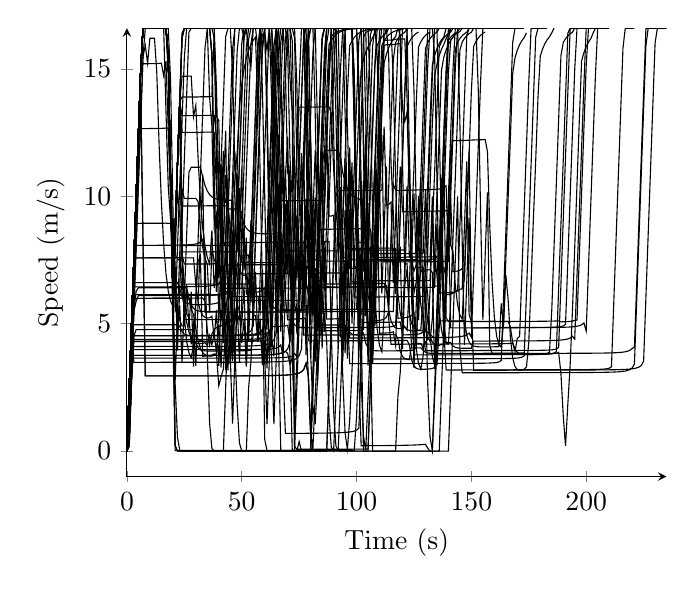
\begin{tikzpicture}
\begin{axis}[
legend style={anchor=west},
axis x line=bottom,
axis y line=left,
ymin=-1,
xlabel=Time (s),
ylabel=Speed (m/s),
]
\addplot[] coordinates {
(0, 0.0)
(1, 1.70108207609)
(2, 4.20108207609)
(3, 6.70108207609)
(4, 9.20108207609)
(5, 11.7010820761)
(6, 14.2010820761)
(7, 8.20108207609)
(8, 2.95038492546)
(9, 2.95041334887)
(10, 2.95044295682)
(11, 2.9504738161)
(12, 2.95050599825)
(13, 2.95053958002)
(14, 2.95057464381)
(15, 2.95061127816)
(16, 2.95064957833)
(17, 2.95068964694)
(18, 2.95073159461)
(19, 2.95077554077)
(20, 2.95082161449)
(21, 2.95086995545)
(22, 2.95092071497)
(23, 2.95097405724)
(24, 2.9510301606)
(25, 2.9510892191)
(26, 2.95115144414)
(27, 2.95121706638)
(28, 2.95128633789)
(29, 2.95135953457)
(30, 2.95143695895)
(31, 2.95151894327)
(32, 2.9516058531)
(33, 2.95169809146)
(34, 2.95179610344)
(35, 2.95190038169)
(36, 2.95201147258)
(37, 2.95212998344)
(38, 2.9522565909)
(39, 2.95239205062)
(40, 2.95253720862)
(41, 2.95269301465)
(42, 2.95286053776)
(43, 2.95304098488)
(44, 2.95323572268)
(45, 2.95344630372)
(46, 2.95367449767)
(47, 2.9539223289)
(48, 2.95419212183)
(49, 2.9544865561)
(50, 2.95480873387)
(51, 2.95516226262)
(52, 2.95555135754)
(53, 2.95598096903)
(54, 2.95645694263)
(55, 2.95698622133)
(56, 2.9575771033)
(57, 2.95823957371)
(58, 2.95898573555)
(59, 2.95983037536)
(60, 2.96079171446)
(61, 2.96189241909)
(62, 2.96316097748)
(63, 2.96463360574)
(64, 2.966801869)
(65, 2.96871538322)
(66, 2.97114643487)
(67, 2.97407974317)
(68, 2.97766601412)
(69, 2.98211811255)
(70, 2.98774528263)
(71, 2.99501216128)
(72, 3.0046461466)
(73, 3.0178462482)
(74, 3.03672593505)
(75, 3.06536813228)
(76, 3.11279808935)
(77, 3.20394948484)
(78, 3.44878428623)
(79, 2.95898349127)
(80, 0.689961382672)
(81, 3.18996138267)
(82, 5.68996138267)
(83, 8.18996138267)
(84, 10.6899613827)
(85, 13.1899613827)
(86, 15.6899613827)
(87, 16.6)
(88, 16.6)
(89, 16.6)
(90, 16.6)
(91, 16.6)
(92, 16.6)
(93, 16.6)
(94, 16.6)
(95, 16.6)
(96, 16.6)
(97, 16.6)
(98, 16.6)
(99, 12.6096433915)
(100, 7.96435127243)
(101, 3.97150395831)
(102, 6.47150395831)
(103, 8.97150395831)
(104, 11.4715039583)
(105, 6.41619497165)
(106, 6.41626596313)
(107, 6.41634220007)
(108, 6.41642421236)
(109, 6.41651259857)
(110, 6.41660803685)
(111, 6.41671129805)
(112, 6.41682326131)
(113, 6.41694493287)
(114, 6.41707746876)
(115, 6.41722220241)
(116, 6.41738067834)
(117, 6.41755469357)
(118, 6.41774634888)
(119, 6.41795811258)
(120, 6.41819290048)
(121, 6.41845417696)
(122, 6.41874608368)
(123, 6.41907360504)
(124, 6.41944278271)
(125, 6.41986099686)
(126, 6.42033733867)
(127, 6.42088310972)
(128, 6.42151250036)
(129, 6.4222435241)
(130, 6.42309932505)
(131, 6.42411003907)
(132, 6.42531549394)
(133, 6.42676921152)
(134, 6.42854448313)
(135, 8.92854448313)
(136, 6.20772617427)
(137, 6.20898912567)
(138, 6.21064762295)
(139, 6.21363768032)
(140, 6.21820084139)
(141, 6.22467630997)
(142, 6.23466962597)
(143, 6.25133301082)
(144, 6.28246751407)
(145, 6.35267516462)
(146, 6.36736269159)
(147, 8.86736269159)
(148, 11.3673626916)
(149, 5.36736269159)
(150, 5.08012960228)
(151, 5.08037635262)
(152, 5.08063888111)
(153, 5.08091856302)
(154, 5.0812169269)
(155, 5.08153567556)
(156, 5.08187671046)
(157, 5.08224216022)
(158, 5.08263441402)
(159, 5.08305616082)
(160, 5.08351043576)
(161, 5.08400067505)
(162, 5.08453078137)
(163, 5.08510520209)
(164, 5.08572902316)
(165, 5.08640808256)
(166, 5.08714910796)
(167, 5.08795988473)
(168, 5.08884946229)
(169, 5.089828409)
(170, 5.09089886235)
(171, 5.09114786172)
(172, 5.09142468357)
(173, 5.09173364064)
(174, 5.09207991663)
(175, 5.09246978661)
(176, 5.09291090555)
(177, 5.09341269014)
(178, 5.09398683021)
(179, 5.09464798275)
(180, 5.09541472726)
(181, 5.09631090185)
(182, 5.0973675047)
(183, 5.09862545345)
(184, 5.10013967802)
(185, 5.1019853435)
(186, 5.10426758218)
(187, 5.1079602043)
(188, 5.11089129401)
(189, 5.07386476251)
(190, 5.07606530746)
(191, 5.07914589033)
(192, 5.08366410048)
(193, 5.09072482581)
(194, 5.10283452185)
(195, 5.12708394722)
(196, 5.14330212083)
(197, 7.64330212083)
(198, 10.1433021208)
(199, 12.6433021208)
(200, 15.1433021208)
(201, 16.6)
(202, 16.6)
(203, 16.6)
(204, 16.6)
(205, 16.6)
(206, 16.6)
};
\addplot[] coordinates {
(0, 0.0)
(1, 2.5)
(2, 5.0)
(3, 7.5)
(4, 10.0)
(5, 12.5)
(6, 15.0)
(7, 16.6)
(8, 16.6)
(9, 16.6)
(10, 16.6)
(11, 16.6)
(12, 16.6)
(13, 16.6)
(14, 16.6)
(15, 16.6)
(16, 16.6)
(17, 16.6)
(18, 15.5220816837)
(19, 10.6413647215)
(20, 6.21632690857)
(21, 0.216326908568)
(22, 0.0)
(23, 0.0)
(24, 0.0)
(25, 0.0)
(26, 0.0)
(27, 0.0)
(28, 0.0)
(29, 0.0)
(30, 0.0)
(31, 0.0)
(32, 0.0)
(33, 0.0)
(34, 0.0)
(35, 0.0)
(36, 0.0)
(37, 0.0)
(38, 0.0)
(39, 0.0)
(40, 0.0)
(41, 0.0)
(42, 0.0)
(43, 0.0)
(44, 0.0)
(45, 0.0)
(46, 0.0)
(47, 0.0)
(48, 0.0)
(49, 0.0)
(50, 0.0)
(51, 0.0)
(52, 0.0)
(53, 0.0)
(54, 0.0)
(55, 0.0)
(56, 0.0)
(57, 0.0)
(58, 0.0)
(59, 0.0)
(60, 0.0)
(61, 0.0)
(62, 0.0)
(63, 0.0)
(64, 0.0)
(65, 0.0)
(66, 0.0)
(67, 0.0)
(68, 0.0)
(69, 0.0)
(70, 0.0)
(71, 0.0)
(72, 0.0)
(73, 0.0)
(74, 0.0)
(75, 0.0)
(76, 0.0)
(77, 0.0)
(78, 0.0)
(79, 0.0)
(80, 0.0)
(81, 2.5)
(82, 5.0)
(83, 7.5)
(84, 10.0)
(85, 12.5)
(86, 15.0)
(87, 16.6)
(88, 16.6)
(89, 16.6)
(90, 16.6)
(91, 16.6)
(92, 16.6)
(93, 16.6)
(94, 16.6)
(95, 16.6)
(96, 16.6)
(97, 16.6)
(98, 16.6)
(99, 14.7741858404)
(100, 8.7741858404)
(101, 2.7741858404)
(102, 0.209867998166)
(103, 0.210326708395)
(104, 0.210812209797)
(105, 0.211326837284)
(106, 0.211873208387)
(107, 0.212454268384)
(108, 0.213073344571)
(109, 0.213734211958)
(110, 0.21444117337)
(111, 0.215199157854)
(112, 0.216013842581)
(113, 0.21689180522)
(114, 0.217840716279)
(115, 0.218869584505)
(116, 0.219989073714)
(117, 0.221211917172)
(118, 0.222553467474)
(119, 0.224032438085)
(120, 0.225671921622)
(121, 0.227500817149)
(122, 0.229555878158)
(123, 0.231884731525)
(124, 0.234550469981)
(125, 0.2376389026)
(126, 0.241270523465)
(127, 0.245621376155)
(128, 0.250961999854)
(129, 0.257736853023)
(130, 0.266746857259)
(131, 0.110669320884)
(132, 0.0)
(133, 0.0)
(134, 2.5)
(135, 5.0)
(136, 7.5)
(137, 10.0)
(138, 12.5)
(139, 15.0)
(140, 16.6)
(141, 16.6)
(142, 16.6)
(143, 16.6)
(144, 16.6)
(145, 16.6)
(146, 16.6)
(147, 16.6)
(148, 16.6)
(149, 16.6)
(150, 16.6)
(151, 16.6)
(152, 16.6)
(153, 14.1874279614)
(154, 9.40399662949)
(155, 5.15505054257)
(156, 7.65505054257)
(157, 10.1550505426)
(158, 4.15505054257)
(159, 3.82912459379)
(160, 3.82925930921)
(161, 3.82940036298)
(162, 3.82954815927)
(163, 3.82970313501)
(164, 3.82986576313)
(165, 3.83003655616)
(166, 3.83021607031)
(167, 3.83040491001)
(168, 3.83060373299)
(169, 3.83081325607)
(170, 3.83103426162)
(171, 3.83126760492)
(172, 3.83151422241)
(173, 3.83177514123)
(174, 3.83205148988)
(175, 3.8323445105)
(176, 3.83265557293)
(177, 3.83298619079)
(178, 3.83333804)
(179, 3.83371298011)
(180, 3.83411307908)
(181, 3.83454064194)
(182, 3.83499824423)
(183, 3.83548877103)
(184, 3.83601546281)
(185, 3.83658196937)
(186, 3.8372737865)
(187, 3.83741086488)
(188, 3.83755915635)
(189, 3.83771992015)
(190, 3.83789459766)
(191, 3.83808484509)
(192, 3.83829257313)
(193, 3.83851999542)
(194, 3.8387696883)
(195, 3.83904466462)
(196, 3.83934846592)
(197, 3.83968527806)
(198, 3.84006007769)
(199, 3.84047881916)
(200, 3.84094867527)
(201, 3.84147835047)
(202, 3.84207849259)
(203, 3.8427622404)
(204, 3.84354596102)
(205, 3.84445025684)
(206, 3.8455013614)
(207, 3.84673310748)
(208, 3.8481897544)
(209, 3.8505696537)
(210, 3.85210426901)
(211, 3.85468952816)
(212, 3.85790605069)
(213, 3.86198151956)
(214, 3.86725891735)
(215, 3.87427661376)
(216, 3.8839243379)
(217, 3.89777408641)
(218, 3.9188680653)
(219, 3.95393437333)
(220, 4.02152298134)
(221, 4.08485509219)
(222, 6.58485509219)
(223, 9.08485509219)
(224, 11.5848550922)
(225, 14.0848550922)
(226, 16.5848550922)
(227, 16.6)
(228, 16.6)
(229, 16.6)
(230, 16.6)
(231, 16.6)
};
\addplot[] coordinates {
(0, 0.0)
(1, 2.5)
(2, 5.0)
(3, 7.5)
(4, 10.0)
(5, 12.5)
(6, 15.0)
(7, 16.6)
(8, 16.6)
(9, 16.6)
(10, 16.6)
(11, 16.6)
(12, 16.6)
(13, 16.6)
(14, 16.6)
(15, 16.6)
(16, 16.6)
(17, 16.6)
(18, 14.9088102554)
(19, 10.8610283475)
(20, 6.40813993979)
(21, 2.77862503402)
(22, 5.27862503402)
(23, 7.77862503402)
(24, 10.278625034)
(25, 9.91960234013)
(26, 9.91969787657)
(27, 9.91980528507)
(28, 9.91992661788)
(29, 9.92006439074)
(30, 9.92022171453)
(31, 9.78825033403)
(32, 8.70026506195)
(33, 7.99930732885)
(34, 7.57733577044)
(35, 7.33193156654)
(36, 5.42686993076)
(37, 7.90274100906)
(38, 7.5196561624)
(39, 7.29943203783)
(40, 7.17625484686)
(41, 7.1085275909)
(42, 7.07171132366)
(43, 7.05206543823)
(44, 7.04159527258)
(45, 7.03624571258)
(46, 8.62270033227)
(47, 6.14361527569)
(48, 7.3731927846)
(49, 7.10764320123)
(50, 6.95573095721)
(51, 6.89149449766)
(52, 6.91533479918)
(53, 5.95111418091)
(54, 7.04576111191)
(55, 5.30164005317)
(56, 5.32255399644)
(57, 4.27602160575)
(58, 5.20497210035)
(59, 3.36220410801)
(60, 5.86220410801)
(61, 8.36220410801)
(62, 10.862204108)
(63, 13.362204108)
(64, 15.862204108)
(65, 16.6)
(66, 16.6)
(67, 16.6)
(68, 16.6)
(69, 16.6)
(70, 16.6)
(71, 16.6)
(72, 16.6)
(73, 16.6)
(74, 16.6)
(75, 16.6)
(76, 16.6)
(77, 16.6)
(78, 13.9271716504)
(79, 9.16463353263)
(80, 4.95401788329)
(81, 7.45401788329)
(82, 9.95401788329)
(83, 4.72331617316)
(84, 4.72351220529)
(85, 4.72371952221)
(86, 4.72393900748)
(87, 4.72417163293)
(88, 4.72441846942)
(89, 4.72468069923)
(90, 4.7249596303)
(91, 4.72525671258)
(92, 4.72557355698)
(93, 4.72591195731)
(94, 4.72627391577)
(95, 4.72666167279)
(96, 4.72707774181)
(97, 4.72752495032)
(98, 4.72800648813)
(99, 4.72852596466)
(100, 4.72908747703)
(101, 4.72969569142)
(102, 4.73035594073)
(103, 4.62917508454)
(104, 4.22846322816)
(105, 4.05350940106)
(106, 3.98127349112)
(107, 3.95226538675)
(108, 3.94082126402)
(109, 3.93641578625)
(110, 3.93482304784)
(111, 3.93436194828)
(112, 3.93436748932)
(113, 3.93457875961)
(114, 3.93489560069)
(115, 3.93528219809)
(116, 3.93572903638)
(117, 3.93623804112)
(118, 3.93681697671)
(119, 3.93747760692)
(120, 3.93823548191)
(121, 3.93911056475)
(122, 3.94012847568)
(123, 3.94132240643)
(124, 3.94273594881)
(125, 3.99478085088)
(126, 4.04507510713)
(127, 6.54507510713)
(128, 7.05142808718)
(129, 7.05855951698)
(130, 7.07103236611)
(131, 6.10872626531)
(132, 4.52203449702)
(133, 3.70791631823)
(134, 3.3960684269)
(135, 3.37991281364)
(136, 4.85694682031)
(137, 7.35694682031)
(138, 9.85694682031)
(139, 12.3569468203)
(140, 14.8569468203)
(141, 16.1326550501)
(142, 16.2589882736)
(143, 16.3507203392)
(144, 16.4175390177)
(145, 16.4663211808)
(146, 16.6)
};
\addplot[] coordinates {
(0, 0.0)
(1, 2.5)
(2, 5.0)
(3, 5.99663531635)
(4, 5.99670123202)
(5, 5.99677184019)
(6, 5.99684759725)
(7, 5.99692901644)
(8, 5.99701667664)
(9, 5.99711123265)
(10, 5.9972134275)
(11, 5.99732410712)
(12, 5.9974442379)
(13, 5.99757492793)
(14, 5.99771745269)
(15, 5.9978732863)
(16, 5.99804413996)
(17, 5.99823200914)
(18, 5.99843923233)
(19, 5.9986685643)
(20, 5.9989232684)
(21, 5.99920723365)
(22, 5.99952512454)
(23, 5.9998825745)
(24, 6.00028643811)
(25, 6.00074512357)
(26, 6.00126903582)
(27, 6.00187117481)
(28, 6.00256795408)
(29, 6.00338033801)
(30, 6.00433544788)
(31, 6.00546887218)
(32, 6.00682805849)
(33, 6.0084774089)
(34, 5.87861952598)
(35, 4.73235642983)
(36, 4.16098050395)
(37, 4.59111196602)
(38, 4.77037530326)
(39, 4.85129517248)
(40, 4.89174561621)
(41, 4.91636944048)
(42, 4.9371447442)
(43, 4.96192739153)
(44, 5.0001215392)
(45, 5.0730216053)
(46, 5.26872893203)
(47, 4.03316960613)
(48, 1.82136025904)
(49, 0.313970486499)
(50, 0.0)
(51, 0.0)
(52, 0.0)
(53, 2.5)
(54, 3.4921372482)
(55, 5.9921372482)
(56, 8.4921372482)
(57, 10.9921372482)
(58, 13.4921372482)
(59, 15.9921372482)
(60, 16.6)
(61, 16.6)
(62, 16.6)
(63, 16.6)
(64, 16.6)
(65, 16.6)
(66, 16.6)
(67, 16.6)
(68, 16.6)
(69, 16.6)
(70, 16.6)
(71, 16.6)
(72, 13.4470251624)
(73, 8.72489340264)
(74, 4.58885097107)
(75, 7.08885097107)
(76, 9.58885097107)
(77, 12.0888509711)
(78, 14.5888509711)
(79, 16.6)
(80, 16.6)
(81, 16.6)
(82, 16.6)
(83, 16.6)
(84, 16.6)
(85, 16.6)
(86, 16.6)
(87, 16.6)
(88, 16.6)
(89, 16.6)
(90, 16.6)
(91, 16.6)
(92, 16.6)
(93, 12.4150130769)
(94, 7.78885599679)
(95, 3.83190102365)
(96, 6.33190102365)
(97, 8.83190102365)
(98, 11.3319010236)
(99, 6.04418674494)
(100, 6.04455211585)
(101, 6.04494595458)
(102, 6.04537129919)
(103, 6.04583160436)
(104, 6.04633081199)
(105, 6.04687343609)
(106, 6.04746466542)
(107, 6.04811048845)
(108, 6.04881784605)
(109, 6.0495948194)
(110, 6.05045086271)
(111, 6.05139709329)
(112, 6.05244665587)
(113, 6.0536151837)
(114, 6.05492138692)
(115, 6.05638781021)
(116, 6.05710964159)
(117, 6.05749965217)
(118, 6.05794422731)
(119, 6.05845406384)
(120, 6.05904262088)
(121, 6.05972702472)
(122, 6.0605293404)
(123, 6.06147839107)
(124, 6.06261241343)
(125, 6.06398302116)
(126, 6.0656612724)
(127, 6.06774723043)
(128, 6.07038553916)
(129, 6.07379180461)
(130, 6.07935358423)
(131, 5.06865418317)
(132, 4.51638182868)
(133, 4.26721875356)
(134, 4.16823810197)
(135, 4.13962260089)
(136, 4.14882890156)
(137, 4.19310839408)
(138, 4.20548533602)
(139, 5.95096869671)
(140, 8.45096869671)
(141, 10.7672880916)
(142, 13.2672880916)
(143, 15.7672880916)
(144, 16.0526546848)
(145, 16.2010748035)
(146, 16.3086266899)
(147, 16.3868556191)
(148, 16.4439086855)
(149, 16.6)
};
\addplot[] coordinates {
(0, 0.0)
(1, 2.5)
(2, 5.0)
(3, 6.13940894832)
(4, 6.13947811607)
(5, 6.13955233268)
(6, 6.13963210192)
(7, 6.13971799206)
(8, 6.13981064596)
(9, 6.13991079323)
(10, 6.14001926459)
(11, 6.14013700921)
(12, 6.14026511559)
(13, 6.14040483684)
(14, 6.1405576215)
(15, 6.1407251513)
(16, 6.14090938777)
(17, 6.14111263003)
(18, 6.14133758704)
(19, 6.14158746859)
(20, 6.14186610076)
(21, 6.14217807369)
(22, 6.1425289325)
(23, 6.14292542625)
(24, 6.14337583627)
(25, 6.14389041393)
(26, 6.14448197191)
(27, 6.1451666937)
(28, 6.14596525867)
(29, 6.146904432)
(30, 6.14801935297)
(31, 6.14935689696)
(32, 6.1509807297)
(33, 6.15297910616)
(34, 6.15547726828)
(35, 6.15865784086)
(36, 6.12986243803)
(37, 6.13185845934)
(38, 6.1354854264)
(39, 6.13929959427)
(40, 6.14525063674)
(41, 6.15490710742)
(42, 6.17229744421)
(43, 6.20949839676)
(44, 6.32441120085)
(45, 3.74749688403)
(46, 1.07415951868)
(47, 3.57415951868)
(48, 6.07415951868)
(49, 8.57415951868)
(50, 11.0741595187)
(51, 7.39512960559)
(52, 7.39514013307)
(53, 7.39515163501)
(54, 7.39516423554)
(55, 7.39517807917)
(56, 7.39519333503)
(57, 7.39521020197)
(58, 7.39522891518)
(59, 7.39524975437)
(60, 7.39527305432)
(61, 7.39529921844)
(62, 7.39532873634)
(63, 7.39536220697)
(64, 7.39540036926)
(65, 7.39544414335)
(66, 7.4023700035)
(67, 7.4023707502)
(68, 7.40237162567)
(69, 7.40237266135)
(70, 7.40237389887)
(71, 7.40237539438)
(72, 7.40237722499)
(73, 7.40237949902)
(74, 7.40197058123)
(75, 7.40267883696)
(76, 7.40268308306)
(77, 7.40268885133)
(78, 9.90268885133)
(79, 7.04839369533)
(80, 7.06093825759)
(81, 7.08195141257)
(82, 7.12200327217)
(83, 7.21519937272)
(84, 5.24109339662)
(85, 7.74109339662)
(86, 10.2410933966)
(87, 12.7410933966)
(88, 15.2410933966)
(89, 16.6)
(90, 16.6)
(91, 16.6)
(92, 16.6)
(93, 16.6)
(94, 16.6)
(95, 16.6)
(96, 16.6)
(97, 16.6)
(98, 16.6)
(99, 16.6)
(100, 16.6)
(101, 16.6)
(102, 16.6)
(103, 11.7261551656)
(104, 7.17204293067)
(105, 3.35083952377)
(106, 5.85083952377)
(107, 8.35083952377)
(108, 10.8508395238)
(109, 13.3508395238)
(110, 15.8508395238)
(111, 16.6)
(112, 16.6)
(113, 16.6)
(114, 16.6)
(115, 16.6)
(116, 16.6)
(117, 16.6)
(118, 16.6)
(119, 16.6)
(120, 16.6)
(121, 16.6)
(122, 16.6)
(123, 16.6)
(124, 16.6)
(125, 16.6)
(126, 16.6)
(127, 16.6)
(128, 16.6)
(129, 16.6)
(130, 16.6)
(131, 16.6)
};
\addplot[] coordinates {
(0, 0.0)
(1, 2.5)
(2, 5.0)
(3, 3.48456527937)
(4, 3.48458711256)
(5, 3.48460982562)
(6, 3.48463346648)
(7, 3.48465808638)
(8, 3.48468374016)
(9, 3.48471048655)
(10, 3.4847383885)
(11, 3.48476751359)
(12, 3.48479793437)
(13, 3.48482972891)
(14, 3.48486298119)
(15, 3.48489778177)
(16, 3.4849342283)
(17, 3.4849724263)
(18, 3.48501248987)
(19, 3.48505454254)
(20, 3.48509871827)
(21, 3.48514516248)
(22, 3.48519403328)
(23, 3.48524550278)
(24, 3.48529975867)
(25, 3.48535700585)
(26, 3.48541746848)
(27, 3.48548139209)
(28, 3.48554904613)
(29, 3.4856207268)
(30, 3.48569676033)
(31, 3.48577750669)
(32, 3.48586336385)
(33, 3.48595477276)
(34, 3.48605222299)
(35, 3.48615625935)
(36, 3.48626748952)
(37, 3.486386593)
(38, 3.48651433153)
(39, 3.48665156135)
(40, 3.48679924765)
(41, 3.48695848164)
(42, 3.48713050088)
(43, 3.48731671347)
(44, 3.48751872713)
(45, 3.48773838418)
(46, 3.48797780394)
(47, 3.48823943429)
(48, 3.48852611494)
(49, 3.48884115525)
(50, 3.48918843087)
(51, 3.4895725044)
(52, 3.48999877722)
(53, 3.49047368208)
(54, 3.49100492949)
(55, 3.49160182583)
(56, 3.49227568823)
(57, 3.4930403914)
(58, 3.49391309696)
(59, 3.49491523869)
(60, 3.49607387227)
(61, 3.49742355304)
(62, 3.49900899372)
(63, 3.50088889816)
(64, 3.50314161152)
(65, 3.50628719953)
(66, 3.50965174111)
(67, 3.51385545334)
(68, 3.51920738871)
(69, 3.52617630644)
(70, 3.53550377157)
(71, 3.54842637816)
(72, 3.56715192376)
(73, 3.59600603347)
(74, 3.64469768801)
(75, 3.74048512631)
(76, 4.00550935564)
(77, 6.50550935564)
(78, 9.00550935564)
(79, 11.5055093556)
(80, 5.50550935564)
(81, 5.47450912484)
(82, 5.47453928333)
(83, 5.47457146213)
(84, 5.47460584583)
(85, 5.47464264062)
(86, 5.47468207736)
(87, 5.47472441523)
(88, 5.474769946)
(89, 5.47481899906)
(90, 5.47487194744)
(91, 5.47492921488)
(92, 5.47499128435)
(93, 5.47505870834)
(94, 5.47513212113)
(95, 5.47521225382)
(96, 5.47529995263)
(97, 5.47539620135)
(98, 5.47550214909)
(99, 5.47561914482)
(100, 5.47574878057)
(101, 5.47851848153)
(102, 5.47856170925)
(103, 5.47861017404)
(104, 5.47866475794)
(105, 5.47872653698)
(106, 5.4787968347)
(107, 5.47887729392)
(108, 5.47896997385)
(109, 5.47907748363)
(110, 5.47920316872)
(111, 5.47935137548)
(112, 5.47988076142)
(113, 5.47987873172)
(114, 5.48013956411)
(115, 5.4804619026)
(116, 5.48086678339)
(117, 7.98086678339)
(118, 5.21449760743)
(119, 5.21919867144)
(120, 5.2257243633)
(121, 5.23516873268)
(122, 5.24932430846)
(123, 5.27318362183)
(124, 5.31701987098)
(125, 5.41357698564)
(126, 4.14846890965)
(127, 6.64846890965)
(128, 9.14846890965)
(129, 11.6484689097)
(130, 14.1484689097)
(131, 16.6)
(132, 16.6)
(133, 16.6)
(134, 16.6)
(135, 16.6)
(136, 16.6)
(137, 16.6)
(138, 16.6)
(139, 16.6)
(140, 16.6)
(141, 16.6)
(142, 16.6)
(143, 16.6)
(144, 16.6)
(145, 12.8786463135)
(146, 8.20772785736)
(147, 4.16694627607)
(148, 6.66694627607)
(149, 9.16694627607)
(150, 4.83502378847)
(151, 4.83522705086)
(152, 4.83544225812)
(153, 4.83567036536)
(154, 4.83591242519)
(155, 4.83616959984)
(156, 4.83644317524)
(157, 4.83673457712)
(158, 4.83704538965)
(159, 4.83737737716)
(160, 4.83773250921)
(161, 4.83811298998)
(162, 4.83852129268)
(163, 4.83896019997)
(164, 4.83943285161)
(165, 4.83994280101)
(166, 4.84049408245)
(167, 4.84109129141)
(168, 4.84173968107)
(169, 4.84244527873)
(170, 4.84321502704)
(171, 4.84405695629)
(172, 4.84498039581)
(173, 4.84568543563)
(174, 4.84591860038)
(175, 4.84617677003)
(176, 4.84646365893)
(177, 4.84678369907)
(178, 4.84714221351)
(179, 4.84754564094)
(180, 4.84800182917)
(181, 4.84852042331)
(182, 4.84911338491)
(183, 4.84979569572)
(184, 4.85058632496)
(185, 4.85150958028)
(186, 4.85259702726)
(187, 4.85389027019)
(188, 4.85544506914)
(189, 4.85733758689)
(190, 4.85967413738)
(191, 4.86345028811)
(192, 4.86643763598)
(193, 4.87136945131)
(194, 4.87801570498)
(195, 4.88729706969)
(196, 4.90087174923)
(197, 4.92201877654)
(198, 4.95816654404)
(199, 5.03033917966)
(200, 4.71137849689)
(201, 7.21137849689)
(202, 9.71137849689)
(203, 12.2113784969)
(204, 14.7113784969)
(205, 16.6)
(206, 16.6)
(207, 16.6)
(208, 16.6)
(209, 16.6)
(210, 16.6)
};
\addplot[] coordinates {
(0, 0.0)
(1, 2.5)
(2, 5.0)
(3, 7.5)
(4, 10.0)
(5, 12.5)
(6, 15.0)
(7, 16.6)
(8, 16.6)
(9, 16.6)
(10, 16.6)
(11, 16.6)
(12, 16.6)
(13, 16.6)
(14, 16.6)
(15, 16.6)
(16, 16.6)
(17, 16.6)
(18, 15.5220816837)
(19, 10.6413647215)
(20, 6.21632690857)
(21, 8.71632690857)
(22, 11.2163269086)
(23, 13.7163269086)
(24, 12.508632187)
(25, 12.5088021199)
(26, 12.5090004057)
(27, 12.5092337229)
(28, 12.50951084)
(29, 12.5098434515)
(30, 12.5102474345)
(31, 12.5107447808)
(32, 12.51136666)
(33, 12.5181336328)
(34, 12.5184101997)
(35, 12.5187791492)
(36, 12.5192867777)
(37, 12.520012532)
(38, 12.5214853952)
(39, 10.2220495072)
(40, 9.24605899892)
(41, 8.61273249921)
(42, 8.22922096986)
(43, 8.01528309213)
(44, 6.24060171429)
(45, 7.89178601467)
(46, 3.91364143498)
(47, 6.41364143498)
(48, 8.91364143498)
(49, 11.413641435)
(50, 13.913641435)
(51, 16.413641435)
(52, 16.6)
(53, 16.6)
(54, 16.6)
(55, 16.6)
(56, 16.6)
(57, 16.6)
(58, 16.6)
(59, 16.6)
(60, 16.6)
(61, 16.6)
(62, 16.6)
(63, 16.6)
(64, 15.0678994822)
(65, 13.5837511574)
(66, 8.84985843392)
(67, 4.69205285716)
(68, 7.19205285716)
(69, 9.69205285716)
(70, 7.23268765866)
(71, 7.23299206496)
(72, 7.23332401873)
(73, 7.23368694904)
(74, 7.23408483601)
(75, 7.23452232059)
(76, 7.23500484092)
(77, 7.23553880254)
(78, 7.23613179276)
(79, 7.23679285247)
(80, 7.23753282403)
(81, 7.23836480025)
(82, 7.15008156)
(83, 6.81520401879)
(84, 6.64085052882)
(85, 6.54284940376)
(86, 6.49132760526)
(87, 6.46452122356)
(88, 6.45070261856)
(89, 6.44367606133)
(90, 6.4402050274)
(91, 6.43861242363)
(92, 6.43803798898)
(93, 6.43805012092)
(94, 6.43844568375)
(95, 6.43914948978)
(96, 6.44016814507)
(97, 6.44157694642)
(98, 6.44235834018)
(99, 6.44515389541)
(100, 6.44935522339)
(101, 6.45607950615)
(102, 6.46794038712)
(103, 6.49256108254)
(104, 5.94499142776)
(105, 8.15113579682)
(106, 10.2140949612)
(107, 12.6343622681)
(108, 15.1206763754)
(109, 15.939077756)
(110, 16.1190912949)
(111, 16.2491596285)
(112, 16.3435715281)
(113, 16.4123254102)
(114, 16.6)
};
\addplot[] coordinates {
(0, 0.0)
(1, 2.5)
(2, 3.65077009539)
(3, 3.65079278904)
(4, 3.65081642431)
(5, 3.65084105402)
(6, 3.65086673479)
(7, 3.65089352728)
(8, 3.65092149664)
(9, 3.65095071283)
(10, 3.6509812511)
(11, 3.65101319247)
(12, 3.65104662427)
(13, 3.65108164071)
(14, 3.65111834359)
(15, 3.65115684301)
(16, 3.65119725822)
(17, 3.65123971851)
(18, 3.6512843643)
(19, 3.65133134826)
(20, 3.64960271197)
(21, 3.64962154685)
(22, 3.64964142272)
(23, 3.64966241778)
(24, 3.64968461769)
(25, 3.6497081165)
(26, 3.64973301761)
(27, 3.64975943493)
(28, 3.64978749418)
(29, 3.64981733439)
(30, 3.64984910964)
(31, 3.64988299107)
(32, 3.64991916913)
(33, 3.64995785638)
(34, 3.64999929051)
(35, 3.65004373811)
(36, 3.65009149893)
(37, 3.65014291095)
(38, 3.65019835645)
(39, 3.65025826915)
(40, 3.65032314269)
(41, 3.65039354098)
(42, 3.65047011046)
(43, 3.65055359512)
(44, 3.65064485468)
(45, 3.65074488701)
(46, 3.65085485561)
(47, 3.65097612385)
(48, 3.65111029766)
(49, 3.65125927944)
(50, 3.65142533628)
(51, 3.65161118751)
(52, 3.65182011769)
(53, 3.65205612417)
(54, 3.65232411171)
(55, 3.65263015238)
(56, 3.65298183689)
(57, 3.6533887565)
(58, 3.65386317412)
(59, 3.6544209752)
(60, 3.65508304105)
(61, 3.6558772751)
(62, 3.65737575185)
(63, 3.65846886937)
(64, 3.65995164283)
(65, 3.66184246537)
(66, 3.66430891582)
(67, 3.66761647588)
(68, 3.67220837364)
(69, 3.67887648726)
(70, 3.68917184289)
(71, 3.70656805874)
(72, 3.74075917789)
(73, 3.83459399911)
(74, 3.70429622769)
(75, 6.20429622769)
(76, 8.70429622769)
(77, 11.2042962277)
(78, 13.7042962277)
(79, 16.2042962277)
(80, 16.6)
(81, 16.6)
(82, 16.6)
(83, 16.6)
(84, 16.6)
(85, 16.6)
(86, 16.6)
(87, 16.6)
(88, 16.6)
(89, 16.6)
(90, 16.6)
(91, 16.6)
(92, 13.2193661935)
(93, 8.51728771357)
(94, 4.41845429974)
(95, 6.91845429974)
(96, 9.41845429974)
(97, 11.9184542997)
(98, 7.88912264962)
(99, 7.88916301987)
(100, 7.88920713186)
(101, 7.88925546281)
(102, 7.88930856852)
(103, 7.88936709943)
(104, 7.8894318207)
(105, 7.8895036373)
(106, 7.88958362589)
(107, 7.88967307545)
(108, 7.88977353958)
(109, 7.8898869045)
(110, 7.89001547836)
(111, 7.89016210983)
(112, 7.8903303475)
(113, 7.89052465699)
(114, 7.89075072092)
(115, 7.89101586006)
(116, 7.89132963491)
(117, 7.89170472208)
(118, 7.8921582188)
(119, 7.89271363301)
(120, 7.89340400416)
(121, 7.89427695511)
(122, 10.3942769551)
(123, 7.62047035343)
(124, 7.62069664578)
(125, 10.1206966458)
(126, 7.2044430321)
(127, 7.20623104712)
(128, 7.20924737666)
(129, 7.21497300344)
(130, 6.18502218762)
(131, 2.61710505108)
(132, 0.545933000603)
(133, 0.0247857091475)
(134, 2.12407621403)
(135, 4.02555234204)
(136, 6.52555234204)
(137, 9.02555234204)
(138, 5.13574875806)
(139, 4.2664398865)
(140, 4.26654670128)
(141, 4.25801545127)
(142, 4.1266496093)
(143, 4.0721925193)
(144, 4.05008188153)
(145, 4.04122563011)
(146, 4.03774382883)
(147, 4.03643458657)
(148, 4.03600533233)
(149, 4.03593586846)
(150, 4.03601734992)
(151, 4.31654803366)
(152, 4.31686794034)
(153, 4.31720900972)
(154, 4.31757315214)
(155, 4.31796249869)
(156, 4.31837943254)
(157, 4.31882662566)
(158, 4.31930708189)
(159, 4.31982418774)
(160, 4.32038177248)
(161, 4.32098417956)
(162, 4.32163635187)
(163, 4.322343934)
(164, 4.32323428581)
(165, 4.32340874845)
(166, 4.32359941611)
(167, 4.32380836316)
(168, 4.32403800748)
(169, 4.32429118117)
(170, 4.32457121893)
(171, 4.32488206922)
(172, 4.3252284354)
(173, 4.32561595627)
(174, 4.32605143921)
(175, 4.32654316429)
(176, 4.32710128532)
(177, 4.3277383647)
(178, 4.32847009628)
(179, 4.32931629578)
(180, 4.33030227904)
(181, 4.33146081319)
(182, 4.3328349318)
(183, 4.33448208464)
(184, 4.33648040454)
(185, 4.33907005379)
(186, 4.34215193118)
(187, 4.34607721139)
(188, 4.35119057256)
(189, 4.35803726696)
(190, 4.36752625543)
(191, 4.38127917622)
(192, 4.40246843643)
(193, 4.43819430521)
(194, 4.50828533238)
(195, 4.39267079592)
(196, 6.89267079592)
(197, 9.39267079592)
(198, 11.8926707959)
(199, 14.3926707959)
(200, 16.6)
(201, 16.6)
(202, 16.6)
(203, 16.6)
(204, 16.6)
(205, 16.6)
};
\addplot[] coordinates {
(0, 0.0)
(1, 2.5)
(2, 5.0)
(3, 6.44637172167)
(4, 6.44644815945)
(5, 6.44653047474)
(6, 6.44661928617)
(7, 6.44671529596)
(8, 6.44681930392)
(9, 6.44693222413)
(10, 6.44705510516)
(11, 6.44718915452)
(12, 6.44733576851)
(13, 6.44749656877)
(14, 6.44767344744)
(15, 6.44786862315)
(16, 6.44808471113)
(17, 6.44832481147)
(18, 6.44859262122)
(19, 6.44889257796)
(20, 6.44923004539)
(21, 6.44961155559)
(22, 6.45004512858)
(23, 6.45054069902)
(24, 6.45111069278)
(25, 6.45177081729)
(26, 6.45254116099)
(27, 6.45344774892)
(28, 6.45452478443)
(29, 6.45581794706)
(30, 6.45738935806)
(31, 6.45932525501)
(32, 6.46174821445)
(33, 6.46483730136)
(34, 6.4688626541)
(35, 6.47424775611)
(36, 6.48264543941)
(37, 6.49307240205)
(38, 6.5093445113)
(39, 6.53589189837)
(40, 6.58406559681)
(41, 6.68832178853)
(42, 6.95993397624)
(43, 3.18916105821)
(44, 5.68916105821)
(45, 8.18916105821)
(46, 10.6891610582)
(47, 13.1891610582)
(48, 15.6891610582)
(49, 16.6)
(50, 16.6)
(51, 16.6)
(52, 16.6)
(53, 16.6)
(54, 16.6)
(55, 16.6)
(56, 16.6)
(57, 16.6)
(58, 16.6)
(59, 16.6)
(60, 16.6)
(61, 13.8580231837)
(62, 9.10115249108)
(63, 4.90096218991)
(64, 7.40096218991)
(65, 9.90096218991)
(66, 12.4009621899)
(67, 6.40096218991)
(68, 5.55282589962)
(69, 5.55288397318)
(70, 5.55294585099)
(71, 5.55301187278)
(72, 5.5530824171)
(73, 5.55315790672)
(74, 5.55323881503)
(75, 5.55332567346)
(76, 5.55341908021)
(77, 5.55351971064)
(78, 5.5536283295)
(79, 5.5537458055)
(80, 5.55387312879)
(81, 5.55401143186)
(82, 5.55416201492)
(83, 5.55432637652)
(84, 5.55450625111)
(85, 5.554703655)
(86, 5.55492094322)
(87, 5.55516088018)
(88, 5.55542672822)
(89, 5.55572235929)
(90, 5.55605239699)
(91, 5.55642239892)
(92, 5.55683909266)
(93, 5.55731068461)
(94, 5.55784726827)
(95, 5.55846137047)
(96, 5.55916869171)
(97, 5.55998912342)
(98, 5.5609481677)
(99, 5.56207895241)
(100, 5.56342514567)
(101, 8.06342514567)
(102, 5.37631261506)
(103, 5.3771779943)
(104, 5.37826395435)
(105, 7.87826395435)
(106, 5.10619051233)
(107, 5.1097583944)
(108, 5.11470131244)
(109, 5.12183758011)
(110, 5.13271010848)
(111, 5.15054030544)
(112, 5.18311672488)
(113, 5.25427849398)
(114, 5.48173038643)
(115, 7.98173038643)
(116, 10.4817303864)
(117, 10.2334019327)
(118, 10.2343639831)
(119, 10.2354536175)
(120, 10.2366944514)
(121, 10.2381158333)
(122, 10.2397546003)
(123, 10.2416574971)
(124, 10.2438845577)
(125, 10.2465139171)
(126, 10.2496487892)
(127, 10.2534278009)
(128, 10.2564944916)
(129, 10.2576826696)
(130, 10.2591785187)
(131, 10.261098556)
(132, 10.2636203913)
(133, 10.2670258188)
(134, 10.2717842744)
(135, 10.2787268508)
(136, 10.2894448862)
(137, 10.3077231425)
(138, 10.3412495973)
(139, 10.4168804007)
(140, 7.51800275599)
(141, 10.018002756)
(142, 12.518002756)
(143, 15.018002756)
(144, 16.6)
(145, 16.6)
(146, 16.6)
(147, 16.6)
(148, 16.6)
(149, 16.6)
};
\addplot[] coordinates {
(0, 0.0)
(1, 0.480740698408)
(2, 2.98074069841)
(3, 5.48074069841)
(4, 7.98074069841)
(5, 10.4807406984)
(6, 12.9807406984)
(7, 15.4807406984)
(8, 16.6)
(9, 16.6)
(10, 16.6)
(11, 16.6)
(12, 16.6)
(13, 16.6)
(14, 16.6)
(15, 16.6)
(16, 16.6)
(17, 16.6)
(18, 16.6)
(19, 14.5625334367)
(20, 9.75015492285)
(21, 5.44838508348)
(22, 7.94838508348)
(23, 10.4483850835)
(24, 12.9483850835)
(25, 15.4483850835)
(26, 16.6)
(27, 16.6)
(28, 16.6)
(29, 16.6)
(30, 16.6)
(31, 16.6)
(32, 16.6)
(33, 16.6)
(34, 16.6)
(35, 16.6)
(36, 16.6)
(37, 16.6)
(38, 16.2189652327)
(39, 11.2932019366)
(40, 6.78813551617)
(41, 9.28813551617)
(42, 11.7881355162)
(43, 7.31156390099)
(44, 7.31164866438)
(45, 7.31174040447)
(46, 7.31183990861)
(47, 7.31194807845)
(48, 7.31206595047)
(49, 7.3121947209)
(50, 7.31233577624)
(51, 7.31249073073)
(52, 7.31266147284)
(53, 7.3128502231)
(54, 7.31305960672)
(55, 7.31329274555)
(56, 7.31355337516)
(57, 7.31384599571)
(58, 7.3141760677)
(59, 7.31455026905)
(60, 7.31497683606)
(61, 7.31546602136)
(62, 7.31603071705)
(63, 7.31668731474)
(64, 7.31745691159)
(65, 7.31836703109)
(66, 7.31945412612)
(67, 7.3207672995)
(68, 7.32237396992)
(69, 7.3243687408)
(70, 9.8243687408)
(71, 7.08259734992)
(72, 7.08411540081)
(73, 7.08617350645)
(74, 7.08993161947)
(75, 7.09610137917)
(76, 7.10546634114)
(77, 7.12124676945)
(78, 7.15115911663)
(79, 7.22003973325)
(80, 6.80343428933)
(81, 9.30343428933)
(82, 11.8034342893)
(83, 8.70448619145)
(84, 8.70518920938)
(85, 8.70597079255)
(86, 8.70684310733)
(87, 8.70782077151)
(88, 8.70892147235)
(89, 8.71016677448)
(90, 8.71158318761)
(91, 8.71320359394)
(92, 8.71506918123)
(93, 8.71723209712)
(94, 8.71975915024)
(95, 8.72273705862)
(96, 8.72411071507)
(97, 8.72499702325)
(98, 8.72607601544)
(99, 8.72740804234)
(100, 8.72907915885)
(101, 8.73121553163)
(102, 8.73400828087)
(103, 8.73775843822)
(104, 8.7084367266)
(105, 8.71095754845)
(106, 8.71310657238)
(107, 8.02352366962)
(108, 6.00788788825)
(109, 4.77244011123)
(110, 4.14838355075)
(111, 3.90511267361)
(112, 5.36020453069)
(113, 7.86020453069)
(114, 10.3602045307)
(115, 12.8602045307)
(116, 15.3602045307)
(117, 16.0397025415)
(118, 16.1917114621)
(119, 16.3018277294)
(120, 16.381903121)
(121, 16.4402929987)
(122, 16.6)
};
\addplot[] coordinates {
(0, 0.0)
(1, 2.5)
(2, 5.0)
(3, 7.5)
(4, 10.0)
(5, 12.5)
(6, 15.0)
(7, 16.6)
(8, 16.6)
(9, 16.6)
(10, 16.6)
(11, 16.6)
(12, 16.6)
(13, 16.6)
(14, 16.6)
(15, 16.6)
(16, 16.6)
(17, 16.6)
(18, 15.5220816837)
(19, 10.6413647215)
(20, 6.21632690857)
(21, 8.71632690857)
(22, 11.2163269086)
(23, 13.7163269086)
(24, 7.71632690857)
(25, 6.55308720883)
(26, 6.55313596327)
(27, 6.55318883252)
(28, 6.5532462931)
(29, 6.55330889258)
(30, 6.5533772627)
(31, 6.55345213536)
(32, 6.55353436233)
(33, 6.55362493958)
(34, 6.55372503765)
(35, 6.5538360397)
(36, 6.55395958959)
(37, 6.55409765319)
(38, 6.55425259718)
(39, 6.55442729135)
(40, 6.55777077319)
(41, 6.55783134555)
(42, 6.55790076889)
(43, 6.55798085686)
(44, 6.55807391299)
(45, 6.55818289873)
(46, 6.55831167267)
(47, 6.55846533809)
(48, 6.55865075844)
(49, 6.55887734069)
(50, 6.55934850967)
(51, 6.55970545264)
(52, 6.56016437573)
(53, 6.56076831226)
(54, 9.06076831226)
(55, 6.22153851093)
(56, 6.23017650515)
(57, 6.24352725621)
(58, 6.26550579851)
(59, 6.30746758505)
(60, 6.40251194975)
(61, 4.76501930443)
(62, 7.26501930443)
(63, 9.76501930443)
(64, 12.2650193044)
(65, 14.7650193044)
(66, 16.6)
(67, 16.6)
(68, 16.6)
(69, 16.6)
(70, 16.6)
(71, 16.6)
(72, 16.6)
(73, 16.6)
(74, 16.6)
(75, 16.6)
(76, 16.6)
(77, 16.6)
(78, 16.6)
(79, 16.6)
(80, 12.2292205637)
(81, 7.62181469537)
(82, 3.70010614636)
(83, 6.20010614636)
(84, 8.70010614636)
(85, 11.2001061464)
(86, 6.55652032156)
(87, 6.5569504531)
(88, 6.5574171041)
(89, 6.55792453162)
(90, 6.55847763207)
(91, 6.55908206004)
(92, 6.55974437384)
(93, 6.56047221469)
(94, 6.56127452874)
(95, 6.56216184429)
(96, 6.56314662019)
(97, 6.56424368725)
(98, 6.56547081233)
(99, 6.56684942546)
(100, 6.56840556654)
(101, 6.5702744002)
(102, 6.5706933989)
(103, 6.57117437163)
(104, 6.57173019759)
(105, 6.57237729226)
(106, 6.57313684311)
(107, 6.57403658179)
(108, 6.5751133773)
(109, 6.57641711726)
(110, 6.57801666793)
(111, 6.58000929721)
(112, 6.58253608342)
(113, 6.31141510995)
(114, 5.5251586613)
(115, 5.11676083672)
(116, 4.92321107945)
(117, 4.83906223865)
(118, 4.80866432437)
(119, 4.80684779814)
(120, 4.82605159358)
(121, 4.87425519666)
(122, 4.74469691902)
(123, 6.56552606031)
(124, 8.99320781581)
(125, 11.1539524057)
(126, 13.6539524057)
(127, 15.8740274582)
(128, 16.0722619535)
(129, 16.215256116)
(130, 16.318927638)
(131, 16.3943608807)
(132, 16.4493890493)
};
\addplot[] coordinates {
(0, 0.0)
(1, 2.5)
(2, 5.0)
(3, 7.5)
(4, 8.07602326782)
(5, 8.07615576383)
(6, 8.07630165355)
(7, 8.07646280578)
(8, 8.07664142714)
(9, 8.07684013813)
(10, 8.07706206999)
(11, 8.07731098902)
(12, 8.07759145774)
(13, 8.07790904596)
(14, 8.07827061006)
(15, 8.07868466718)
(16, 8.07916190287)
(17, 8.07971586958)
(18, 8.080363963)
(19, 8.08112880979)
(20, 8.08204027829)
(21, 8.08313845377)
(22, 8.08447814705)
(23, 8.08613591291)
(24, 8.08822131694)
(25, 8.09089567612)
(26, 8.09440455175)
(27, 8.09913692973)
(28, 8.10573961193)
(29, 8.11535519313)
(30, 8.13116232601)
(31, 8.1558346093)
(32, 8.20177773661)
(33, 8.30488509824)
(34, 7.73950641768)
(35, 3.7928524746)
(36, 1.09829063184)
(37, 0.0996919850099)
(38, 0.0)
(39, 0.0)
(40, 0.0)
(41, 0.0)
(42, 0.0)
(43, 2.5)
(44, 5.0)
(45, 7.5)
(46, 10.0)
(47, 6.39017591961)
(48, 6.39021552535)
(49, 6.39025821108)
(50, 6.39030430468)
(51, 6.39035417891)
(52, 6.3904082589)
(53, 6.3904670313)
(54, 6.39053105524)
(55, 6.39060097571)
(56, 6.39067753989)
(57, 6.39076161719)
(58, 6.39085422411)
(59, 6.39095655508)
(60, 6.39107002129)
(61, 6.39119629962)
(62, 6.39133739508)
(63, 6.39149572098)
(64, 6.39474372674)
(65, 6.39479803686)
(66, 6.39485990355)
(67, 6.39493079757)
(68, 6.39501256601)
(69, 6.39510755418)
(70, 6.39521877612)
(71, 6.39535015749)
(72, 6.39550688804)
(73, 6.39569594424)
(74, 6.39633933049)
(75, 6.3963697005)
(76, 6.39673317367)
(77, 6.39720022595)
(78, 6.39781444771)
(79, 8.89781444771)
(80, 6.05962408672)
(81, 6.06838557076)
(82, 6.08190491224)
(83, 6.10412772839)
(84, 6.14640453312)
(85, 6.24176152917)
(86, 4.66777915205)
(87, 7.16777915205)
(88, 9.66777915205)
(89, 12.167779152)
(90, 14.667779152)
(91, 16.6)
(92, 16.6)
(93, 16.6)
(94, 16.6)
(95, 16.6)
(96, 16.6)
(97, 16.6)
(98, 16.6)
(99, 16.6)
(100, 16.6)
(101, 16.6)
(102, 16.6)
(103, 16.6)
(104, 16.6)
(105, 12.3317964999)
(106, 7.71397844957)
(107, 3.77268967687)
(108, 6.27268967687)
(109, 8.77268967687)
(110, 11.2726896769)
(111, 13.7726896769)
(112, 16.2726896769)
(113, 16.6)
(114, 16.6)
(115, 16.6)
(116, 16.6)
(117, 16.6)
(118, 16.6)
(119, 16.6)
(120, 16.6)
(121, 16.6)
(122, 16.6)
(123, 16.6)
(124, 16.6)
(125, 16.6)
(126, 16.6)
(127, 16.6)
(128, 16.6)
(129, 16.6)
(130, 16.6)
(131, 16.6)
(132, 16.6)
(133, 16.6)
};
\addplot[] coordinates {
(0, 0.0)
(1, 2.5)
(2, 4.30909489415)
(3, 4.30912666651)
(4, 4.30916000532)
(5, 4.30919501531)
(6, 4.30923181011)
(7, 4.30927051317)
(8, 4.30931125881)
(9, 4.30935419338)
(10, 4.30939947658)
(11, 4.30944728297)
(12, 4.30949780361)
(13, 4.30955124802)
(14, 4.30960784633)
(15, 4.30966785179)
(16, 4.30973154359)
(17, 4.30979923013)
(18, 4.30987125278)
(19, 4.30994799017)
(20, 4.3100298632)
(21, 4.31011734085)
(22, 4.31021094692)
(23, 4.31031126788)
(24, 4.31041896215)
(25, 4.3105347709)
(26, 4.31065953092)
(27, 4.3107941898)
(28, 4.31093982402)
(29, 4.3110976606)
(30, 4.24203748568)
(31, 4.05503494686)
(32, 3.97770333408)
(33, 3.94665812034)
(34, 3.93442847302)
(35, 3.92973509536)
(36, 3.92805104958)
(37, 3.92757732508)
(38, 3.92760328282)
(39, 3.92785064974)
(40, 3.92821297455)
(41, 3.92865253467)
(42, 3.9291597168)
(43, 3.92973718769)
(44, 3.93039395175)
(45, 3.93114342737)
(46, 3.93200326452)
(47, 3.93299606765)
(48, 3.93415079149)
(49, 3.93550486955)
(50, 3.93710733875)
(51, 3.93902345333)
(52, 3.94134163251)
(53, 3.94454838009)
(54, 3.94813452046)
(55, 4.55100053609)
(56, 4.55410174892)
(57, 4.55846956086)
(58, 4.56492331695)
(59, 4.57510274425)
(60, 4.59277204336)
(61, 4.62873456353)
(62, 4.73220336638)
(63, 3.72105962237)
(64, 1.06019013294)
(65, 3.56019013294)
(66, 6.06019013294)
(67, 8.56019013294)
(68, 11.0601901329)
(69, 6.98578351145)
(70, 6.98579286913)
(71, 6.98580304119)
(72, 6.98581412495)
(73, 6.98582623274)
(74, 6.98583949473)
(75, 6.98585406248)
(76, 6.98587011323)
(77, 6.98588785541)
(78, 6.98590753537)
(79, 6.98592944602)
(80, 6.98595393782)
(81, 6.98598143289)
(82, 6.98601244331)
(83, 6.98604759524)
(84, 6.9923463165)
(85, 6.99234690006)
(86, 6.99234757359)
(87, 6.9923483566)
(88, 6.99234927418)
(89, 6.99235035908)
(90, 6.99235165462)
(91, 6.99235321916)
(92, 6.99235513277)
(93, 6.99235750778)
(94, 6.99258940396)
(95, 6.99259275601)
(96, 6.99259717457)
(97, 9.49259717457)
(98, 6.63403050514)
(99, 6.63621409287)
(100, 6.63960214691)
(101, 6.64741954988)
(102, 6.65814734155)
(103, 6.68266165251)
(104, 5.29565116661)
(105, 7.79565116661)
(106, 10.2956511666)
(107, 12.7956511666)
(108, 15.2956511666)
(109, 16.6)
(110, 16.6)
(111, 16.6)
(112, 16.6)
(113, 16.6)
(114, 16.6)
(115, 16.6)
(116, 16.6)
(117, 16.6)
(118, 16.6)
(119, 16.6)
(120, 16.6)
(121, 16.6)
(122, 16.5497819342)
(123, 11.6038428211)
(124, 7.06327555466)
(125, 3.26767832637)
(126, 5.76767832637)
(127, 8.26767832637)
(128, 10.7676783264)
(129, 4.76767832637)
(130, 3.93733351276)
(131, 3.93743700918)
(132, 3.93754570955)
(133, 3.93765996887)
(134, 3.93778017298)
(135, 3.93790674183)
(136, 3.9380401331)
(137, 3.93818084641)
(138, 3.93832942801)
(139, 3.93848647607)
(140, 3.93865264678)
(141, 3.93882866118)
(142, 3.93901531306)
(143, 3.93921347791)
(144, 3.93942412329)
(145, 3.93964832068)
(146, 3.93988725915)
(147, 3.94014226129)
(148, 3.94041480153)
(149, 3.94070652766)
(150, 3.9410192859)
(151, 3.94135515025)
(152, 3.94171645719)
(153, 3.9421058466)
(154, 3.94839672299)
(155, 3.94844528351)
(156, 3.94849793836)
(157, 3.94855516187)
(158, 3.9486174992)
(159, 3.94868557948)
(160, 3.94876013185)
(161, 3.9488420052)
(162, 3.94893219263)
(163, 3.94903186195)
(164, 3.94914239399)
(165, 3.94926543118)
(166, 3.94940293946)
(167, 3.94955728826)
(168, 3.94973135439)
(169, 3.94992865883)
(170, 3.95015354873)
(171, 3.95041144263)
(172, 3.95070916552)
(173, 3.95105541367)
(174, 3.95146141039)
(175, 3.95194184869)
(176, 3.9525162753)
(177, 3.95249666279)
(178, 3.95335500326)
(179, 3.95442389961)
(180, 3.95577957033)
(181, 3.95753692035)
(182, 3.9598764306)
(183, 3.96309649459)
(184, 3.96772430926)
(185, 3.97477929344)
(186, 3.98651084917)
(187, 4.00908997862)
(188, 4.06926953)
(189, 6.56926953)
(190, 9.06926953)
(191, 11.56926953)
(192, 14.06926953)
(193, 16.56926953)
(194, 16.6)
(195, 16.6)
(196, 16.6)
(197, 16.6)
(198, 16.6)
};
\addplot[] coordinates {
(0, 0.0)
(1, 2.5)
(2, 5.0)
(3, 6.61165906614)
(4, 6.61173957648)
(5, 6.61182644734)
(6, 6.61192036703)
(7, 6.6120221196)
(8, 6.61213260128)
(9, 6.61225284029)
(10, 6.6123840209)
(11, 6.61252751276)
(12, 6.61268490686)
(13, 6.61285805986)
(14, 6.61304914928)
(15, 6.6132607424)
(16, 6.61349588314)
(17, 6.61375820243)
(18, 6.61405205961)
(19, 6.61438272522)
(20, 6.61475661976)
(21, 6.61518162879)
(22, 6.61566752365)
(23, 6.37572934635)
(24, 6.06142858014)
(25, 5.89864262032)
(26, 5.81697245361)
(27, 5.77692053137)
(28, 5.75778611885)
(29, 5.74911236873)
(30, 5.7457320758)
(31, 5.74514446788)
(32, 5.74618787128)
(33, 5.74838892607)
(34, 5.75165948972)
(35, 5.75617995376)
(36, 5.76276633896)
(37, 5.77172842701)
(38, 5.78474385096)
(39, 5.80502713704)
(40, 5.83980000514)
(41, 5.14357878278)
(42, 6.14673351098)
(43, 4.72414176115)
(44, 5.67273758571)
(45, 3.39611350096)
(46, 5.89611350096)
(47, 8.39611350096)
(48, 10.896113501)
(49, 5.45551918255)
(50, 5.4555245072)
(51, 5.4555301807)
(52, 5.45553623423)
(53, 5.4555427025)
(54, 5.45554962429)
(55, 5.45555704303)
(56, 5.45556500745)
(57, 5.45557357243)
(58, 5.45558279992)
(59, 5.45559276007)
(60, 5.45560353257)
(61, 5.45561520826)
(62, 5.45562789101)
(63, 5.45564170012)
(64, 5.45565677306)
(65, 5.45567326897)
(66, 5.45569137282)
(67, 5.45571130071)
(68, 5.45573330626)
(69, 5.45575768881)
(70, 5.46081598309)
(71, 5.46081636761)
(72, 5.4608167987)
(73, 5.46081728421)
(74, 5.46081783372)
(75, 5.46081845897)
(76, 5.46081917459)
(77, 5.46081999887)
(78, 5.46082095502)
(79, 5.46082207277)
(80, 5.46082339076)
(81, 5.4605227278)
(82, 5.46102826462)
(83, 5.46103026303)
(84, 5.46103273251)
(85, 5.46103583411)
(86, 7.96103583411)
(87, 5.18210102808)
(88, 5.1833367392)
(89, 5.18505150521)
(90, 5.18753207293)
(91, 5.19302288021)
(92, 5.19925245559)
(93, 5.21067608705)
(94, 2.93472268133)
(95, 0.706419098523)
(96, 0.0726894273433)
(97, 1.22301064682)
(98, 3.14671274795)
(99, 5.23543498137)
(100, 7.73543498137)
(101, 10.2354349814)
(102, 12.7354349814)
(103, 16.2223691701)
(104, 16.4343850893)
(105, 16.4786345951)
(106, 16.5110061552)
(107, 16.5347137603)
(108, 16.5520899061)
(109, 16.5648328215)
(110, 16.5741818546)
(111, 16.5810430261)
(112, 16.5860795145)
(113, 16.5897771937)
(114, 16.5924922781)
(115, 16.594486053)
(116, 14.5845664024)
(117, 10.6705496364)
(118, 7.07185053845)
(119, 8.0208992627)
(120, 4.01672725906)
(121, 6.51672725906)
(122, 7.14876949857)
(123, 5.53499098631)
(124, 4.05208683174)
(125, 4.05223460656)
(126, 4.0523897001)
(127, 4.05255260403)
(128, 4.05272385201)
(129, 3.961802781)
(130, 3.88234487334)
(131, 3.85088049422)
(132, 3.83865029634)
(133, 3.83400463886)
(134, 3.83233455644)
(135, 3.83183395005)
(136, 3.83179806117)
(137, 3.83195271857)
(138, 3.83219180871)
(139, 3.83247481227)
(140, 3.83278686214)
(141, 3.83312318699)
(142, 3.83348306186)
(143, 3.83386746578)
(144, 3.83427818645)
(145, 3.83471749171)
(146, 3.83518802533)
(147, 3.83569279428)
(148, 3.83623519669)
(149, 3.83686870514)
(150, 3.83719939002)
(151, 3.83741881974)
(152, 3.83760246401)
(153, 3.83778063608)
(154, 3.83796616948)
(155, 3.83816523523)
(156, 3.83838159038)
(157, 3.83861827154)
(158, 3.8388783004)
(159, 3.8391650152)
(160, 3.83948227046)
(161, 3.83983460417)
(162, 3.84022741695)
(163, 3.84066718862)
(164, 3.84116175354)
(165, 3.84172065891)
(166, 3.84235563805)
(167, 3.84308124428)
(168, 3.84391571135)
(169, 3.8448821391)
(170, 3.84601015403)
(171, 3.84733827781)
(172, 3.84930696386)
(173, 3.85101087859)
(174, 3.78978099789)
(175, 3.79069046068)
(176, 3.79188343526)
(177, 3.79343285706)
(178, 3.7954767553)
(179, 3.79824944619)
(180, 3.80215992407)
(181, 3.80797909044)
(182, 3.8173496227)
(183, 3.83457096608)
(184, 3.87705478813)
(185, 5.52111571931)
(186, 8.02111571931)
(187, 10.5211157193)
(188, 13.0211157193)
(189, 15.5211157193)
(190, 16.0369234386)
(191, 16.1897028682)
(192, 16.3003694803)
(193, 16.3808410297)
(194, 16.4395176606)
(195, 16.6)
};
\addplot[] coordinates {
(0, 0.0)
(1, 2.5)
(2, 4.10710922702)
(3, 4.10713804689)
(4, 4.10716821827)
(5, 4.10719982704)
(6, 4.107232966)
(7, 4.10726773556)
(8, 4.10730424452)
(9, 4.10734261092)
(10, 4.10738296296)
(11, 4.10742544011)
(12, 4.10747019433)
(13, 4.10751739139)
(14, 4.10756721244)
(15, 4.10761985575)
(16, 4.10767553866)
(17, 4.1077344999)
(18, 4.10779700206)
(19, 4.10786333462)
(20, 4.10793381725)
(21, 4.1080088037)
(22, 4.10808868625)
(23, 4.10817390088)
(24, 4.10826493322)
(25, 4.1083623255)
(26, 4.1084666847)
(27, 4.108578692)
(28, 4.10869911401)
(29, 4.10882881592)
(30, 4.10896877715)
(31, 4.10912010993)
(32, 4.10928408159)
(33, 4.1094621412)
(34, 4.10965595188)
(35, 4.10986742993)
(36, 4.11009879251)
(37, 4.11035261634)
(38, 4.11063191007)
(39, 4.11094020429)
(40, 4.11128166429)
(41, 4.11166123234)
(42, 4.11208480867)
(43, 4.11255948377)
(44, 4.11309383923)
(45, 4.11369834157)
(46, 4.11438586326)
(47, 4.11517238034)
(48, 4.11607791902)
(49, 4.11712785826)
(50, 4.11835475105)
(51, 4.1198009157)
(52, 4.12152219523)
(53, 4.12359353203)
(54, 4.1261174417)
(55, 4.12923726254)
(56, 4.13365588595)
(57, 4.13869021479)
(58, 4.14529716869)
(59, 4.15422115166)
(60, 4.16671809117)
(61, 4.18506006539)
(62, 4.21376526384)
(63, 4.26314474846)
(64, 4.36267810375)
(65, 4.64696685357)
(66, 7.14696685357)
(67, 9.64696685357)
(68, 12.1469668536)
(69, 14.6469668536)
(70, 16.6)
(71, 16.6)
(72, 16.6)
(73, 16.6)
(74, 16.6)
(75, 16.6)
(76, 16.6)
(77, 16.6)
(78, 16.6)
(79, 16.6)
(80, 16.6)
(81, 16.6)
(82, 16.6)
(83, 12.6774392632)
(84, 8.02560038905)
(85, 4.02049208396)
(86, 6.52049208396)
(87, 9.02049208396)
(88, 11.520492084)
(89, 14.020492084)
(90, 16.520492084)
(91, 16.6)
(92, 16.6)
(93, 16.6)
(94, 16.6)
(95, 16.6)
(96, 16.6)
(97, 16.6)
(98, 16.6)
(99, 16.6)
(100, 16.6)
(101, 16.6)
(102, 16.6)
(103, 16.6)
(104, 13.0382465464)
(105, 8.35255632295)
(106, 4.28422078371)
(107, 0.0)
(108, 0.0)
(109, 0.0)
(110, 0.0)
(111, 0.0)
(112, 0.0)
(113, 0.0)
(114, 0.0)
(115, 0.0)
(116, 0.0)
(117, 0.0)
(118, 0.0)
(119, 0.0)
(120, 0.0)
(121, 0.0)
(122, 0.0)
(123, 0.0)
(124, 0.0)
(125, 0.0)
(126, 0.0)
(127, 0.0)
(128, 0.0)
(129, 0.0)
(130, 0.0)
(131, 0.0)
(132, 0.0)
(133, 0.0)
(134, 0.0)
(135, 0.0)
(136, 0.0)
(137, 0.0)
(138, 0.0)
(139, 0.0)
(140, 0.0)
(141, 2.5)
(142, 5.0)
(143, 7.5)
(144, 10.0)
(145, 4.0)
(146, 3.07280071886)
(147, 3.07289535557)
(148, 3.07299365079)
(149, 3.07309579565)
(150, 3.07320199396)
(151, 3.07331246318)
(152, 3.07342743558)
(153, 3.07354715944)
(154, 3.0736719004)
(155, 3.07380194294)
(156, 3.07393759202)
(157, 3.07407917484)
(158, 3.07422704285)
(159, 3.07438157395)
(160, 3.07454317488)
(161, 3.07471228391)
(162, 3.07488937385)
(163, 3.07507495537)
(164, 3.07526958067)
(165, 3.07547384761)
(166, 3.07568840435)
(167, 3.0759139545)
(168, 3.07615126292)
(169, 3.07640116222)
(170, 3.07666456015)
(171, 3.07694244785)
(172, 3.07723590924)
(173, 3.07754613166)
(174, 3.07787441796)
(175, 3.07822220025)
(176, 3.07859105566)
(177, 3.07909076349)
(178, 3.07917737199)
(179, 3.07926956792)
(180, 3.07936784318)
(181, 3.07947274512)
(182, 3.0795848842)
(183, 3.07970494298)
(184, 3.07983368655)
(185, 3.07997197488)
(186, 3.08012077729)
(187, 3.08028118966)
(188, 3.08045445475)
(189, 3.08064198663)
(190, 3.08084539985)
(191, 3.0810665446)
(192, 3.08130754945)
(193, 3.08157087322)
(194, 3.08185936873)
(195, 3.08217636132)
(196, 3.08252574638)
(197, 3.08291211123)
(198, 3.0833408888)
(199, 3.08381855277)
(200, 3.08435286765)
(201, 3.08495321234)
(202, 3.0856310031)
(203, 3.0864002526)
(204, 3.08727831802)
(205, 3.0882869156)
(206, 3.08997636731)
(207, 3.09087712881)
(208, 3.09248076385)
(209, 3.09438440569)
(210, 3.09666908859)
(211, 3.09944572118)
(212, 3.10286965969)
(213, 3.10716453428)
(214, 3.1126629251)
(215, 3.11987956281)
(216, 3.12965203385)
(217, 3.14343530635)
(218, 3.16399361563)
(219, 3.19732074214)
(220, 3.25960807322)
(221, 3.42039309602)
(222, 5.92039309602)
(223, 8.42039309602)
(224, 10.920393096)
(225, 13.420393096)
(226, 15.920393096)
(227, 16.6)
(228, 16.6)
(229, 16.6)
(230, 16.6)
(231, 16.6)
};
\addplot[] coordinates {
(0, 0.0)
(1, 2.5)
(2, 5.0)
(3, 7.5)
(4, 10.0)
(5, 12.5)
(6, 15.0)
(7, 16.6)
(8, 16.6)
(9, 16.6)
(10, 16.6)
(11, 16.6)
(12, 16.6)
(13, 16.6)
(14, 16.6)
(15, 16.6)
(16, 16.6)
(17, 16.6)
(18, 15.5220816837)
(19, 10.6413647215)
(20, 6.21632690857)
(21, 0.216326908568)
(22, 0.0)
(23, 0.0)
(24, 0.0)
(25, 0.0)
(26, 0.0)
(27, 0.0)
(28, 0.0)
(29, 0.0)
(30, 0.0)
(31, 0.0)
(32, 0.0)
(33, 0.0)
(34, 0.0)
(35, 0.0)
(36, 0.0)
(37, 0.0)
(38, 0.0)
(39, 0.0)
(40, 0.0)
(41, 0.0)
(42, 0.0)
(43, 0.0)
(44, 0.0)
(45, 0.0)
(46, 0.0)
(47, 0.0)
(48, 0.0)
(49, 0.0)
(50, 0.0)
(51, 0.0)
(52, 0.0)
(53, 0.0)
(54, 0.0)
(55, 0.0)
(56, 0.0)
(57, 0.0)
(58, 0.0)
(59, 0.0)
(60, 0.0)
(61, 0.0)
(62, 0.0)
(63, 0.0)
(64, 0.0)
(65, 0.0)
(66, 0.0)
(67, 0.0)
(68, 0.0)
(69, 0.0)
(70, 0.0)
(71, 0.0)
(72, 0.0)
(73, 0.0)
(74, 0.0)
(75, 0.0)
(76, 0.0)
(77, 0.0)
(78, 0.0)
(79, 0.0)
(80, 0.0)
(81, 2.5)
(82, 5.0)
(83, 7.5)
(84, 10.0)
(85, 12.5)
(86, 15.0)
(87, 16.6)
(88, 16.6)
(89, 16.6)
(90, 16.6)
(91, 16.6)
(92, 16.6)
(93, 16.6)
(94, 16.6)
(95, 16.6)
(96, 16.6)
(97, 16.6)
(98, 16.6)
(99, 14.7741858404)
(100, 9.94605177612)
(101, 5.61567673161)
(102, 8.11567673161)
(103, 10.6156767316)
(104, 7.74920897271)
(105, 7.74930334203)
(106, 7.74940594449)
(107, 7.7495177666)
(108, 7.74963994722)
(109, 7.7497738067)
(110, 7.74992088268)
(111, 7.75008297455)
(112, 7.75026219873)
(113, 7.75046105822)
(114, 7.75068253056)
(115, 7.75093018001)
(116, 7.75120830208)
(117, 7.75152211128)
(118, 7.75187798764)
(119, 7.75228380411)
(120, 7.75274936644)
(121, 7.7532870122)
(122, 7.75391243835)
(123, 7.75464586253)
(124, 7.75551368186)
(125, 7.75655088829)
(126, 7.75780466315)
(127, 7.75933985831)
(128, 7.76124758874)
(129, 7.76365913539)
(130, 10.2636591354)
(131, 7.49471858701)
(132, 7.4967007362)
(133, 9.9967007362)
(134, 7.09202338193)
(135, 7.10139114207)
(136, 7.11717557881)
(137, 7.14709367398)
(138, 7.21598125932)
(139, 6.80143527757)
(140, 9.30143527757)
(141, 11.8014352776)
(142, 12.1861929834)
(143, 12.1876108774)
(144, 12.1892597154)
(145, 12.1911925584)
(146, 12.1934786443)
(147, 12.1962096952)
(148, 12.1995092949)
(149, 12.2035471751)
(150, 12.2085615877)
(151, 12.2135221757)
(152, 12.2152199699)
(153, 12.2174601067)
(154, 12.2205016696)
(155, 12.2247799352)
(156, 12.2310734393)
(157, 11.7558457624)
(158, 8.84076935511)
(159, 6.66284685555)
(160, 5.26013040558)
(161, 4.50725528605)
(162, 4.1818062127)
(163, 4.08209076635)
(164, 5.01708664064)
(165, 7.51708664064)
(166, 9.92029371888)
(167, 12.3354609397)
(168, 14.8354609397)
(169, 15.4467999918)
(170, 15.7386400768)
(171, 15.9540842001)
(172, 16.1144008664)
(173, 16.234336663)
(174, 16.4172562768)
};
\addplot[] coordinates {
(0, 0.0)
(1, 2.5)
(2, 4.38091194544)
(3, 4.38094480337)
(4, 4.38097930949)
(5, 4.38101557593)
(6, 4.38105372454)
(7, 4.38109388788)
(8, 4.38113621042)
(9, 4.3811808498)
(10, 4.38122797834)
(11, 4.38127778467)
(12, 4.38133047564)
(13, 4.3813862785)
(14, 4.38144544329)
(15, 4.38150824574)
(16, 4.38157499043)
(17, 4.3816460145)
(18, 4.38172169195)
(19, 4.38180243858)
(20, 4.38188871769)
(21, 4.38198104682)
(22, 4.38208000547)
(23, 4.38218624429)
(24, 4.3823004958)
(25, 4.38242358712)
(26, 4.38255645497)
(27, 4.38270016363)
(28, 4.38285592637)
(29, 4.38302513124)
(30, 4.38320937218)
(31, 4.38341048685)
(32, 4.38363060278)
(33, 4.38387219412)
(34, 4.38413815175)
(35, 4.3844318706)
(36, 4.37857176891)
(37, 4.37870249086)
(38, 4.37884845465)
(39, 4.37901212973)
(40, 4.37919650772)
(41, 4.37940524108)
(42, 4.37964282676)
(43, 4.3799148525)
(44, 4.38022833139)
(45, 4.38059216312)
(46, 4.3810177798)
(47, 4.38152006646)
(48, 4.38211869896)
(49, 4.3828401318)
(50, 4.38372062587)
(51, 4.38481099297)
(52, 4.38682460573)
(53, 4.38847380091)
(54, 4.39079086477)
(55, 4.39392986058)
(56, 4.39834062303)
(57, 4.40483946266)
(58, 4.41505414491)
(59, 4.43270569429)
(60, 4.4684216174)
(61, 4.57035319504)
(62, 3.71814486489)
(63, 6.21814486489)
(64, 8.71814486489)
(65, 11.2181448649)
(66, 9.83191858247)
(67, 9.83193664369)
(68, 9.8319569487)
(69, 9.83197988524)
(70, 9.83200592862)
(71, 9.83203566653)
(72, 9.83206983256)
(73, 9.83210935189)
(74, 9.83215540468)
(75, 9.83220951533)
(76, 9.83227368044)
(77, 9.83235055599)
(78, 9.84174638409)
(79, 9.84174783786)
(80, 9.84174965083)
(81, 9.84175195201)
(82, 9.84175493407)
(83, 9.84175889516)
(84, 9.84207919053)
(85, 9.84208587902)
(86, 9.84209584039)
(87, 12.3420958404)
(88, 9.21967675881)
(89, 9.22898296295)
(90, 9.25623463319)
(91, 6.60897430543)
(92, 9.10897430543)
(93, 11.6089743054)
(94, 14.1089743054)
(95, 16.6)
(96, 16.6)
(97, 16.6)
(98, 16.6)
(99, 16.6)
(100, 16.6)
(101, 16.6)
(102, 16.6)
(103, 16.6)
(104, 16.6)
(105, 16.6)
(106, 16.6)
(107, 16.6)
(108, 16.6)
(109, 15.4754619595)
(110, 10.5978891086)
(111, 6.17847500952)
(112, 8.67847500952)
(113, 11.1784750095)
(114, 5.17847500952)
(115, 4.19507106404)
(116, 4.19517941132)
(117, 4.19529341519)
(118, 4.1954134766)
(119, 4.19554003266)
(120, 4.19567356069)
(121, 4.19581458268)
(122, 4.19596367045)
(123, 4.19612145144)
(124, 4.19628861538)
(125, 4.1964659218)
(126, 4.19665420877)
(127, 4.19685440279)
(128, 4.19706753027)
(129, 4.19729473075)
(130, 4.19753727222)
(131, 4.19779656889)
(132, 4.19807420196)
(133, 4.19837194383)
(134, 4.19869178662)
(135, 4.19903597567)
(136, 4.19940704928)
(137, 4.19980788579)
(138, 4.20024175993)
(139, 4.20074776752)
(140, 4.20725444101)
(141, 4.20731396834)
(142, 4.20737901155)
(143, 4.207450275)
(144, 4.20752857936)
(145, 4.2076148856)
(146, 4.20771032471)
(147, 4.20781623533)
(148, 4.20793421128)
(149, 4.20806616244)
(150, 4.20821439329)
(151, 4.20838170529)
(152, 4.20857153175)
(153, 4.20878811762)
(154, 4.20903676215)
(155, 4.20932415117)
(156, 4.2096588189)
(157, 4.21005180093)
(158, 4.21051757518)
(159, 4.21107544684)
(160, 4.21161380543)
(161, 4.21181729373)
(162, 4.21286228294)
(163, 4.21419136594)
(164, 4.2159198216)
(165, 4.2182294948)
(166, 4.2214224825)
(167, 4.22603541836)
(168, 4.23311228909)
(169, 3.90979145033)
(170, 4.43346908874)
(171, 4.49694947173)
(172, 6.99694947173)
(173, 9.49694947173)
(174, 11.9969494717)
(175, 14.4969494717)
(176, 16.6)
(177, 16.6)
(178, 16.6)
(179, 16.6)
(180, 16.6)
(181, 16.6)
};
\addplot[] coordinates {
(0, 0.0)
(1, 0.480740698408)
(2, 2.98074069841)
(3, 5.48074069841)
(4, 7.98074069841)
(5, 10.4807406984)
(6, 12.9807406984)
(7, 15.4807406984)
(8, 15.9264852882)
(9, 15.2262094002)
(10, 16.2065413759)
(11, 16.2071126122)
(12, 16.2078738906)
(13, 14.8699569287)
(14, 12.0611771086)
(15, 9.80254386604)
(16, 8.11432392303)
(17, 6.97420492403)
(18, 6.27944594571)
(19, 5.89142471891)
(20, 5.68821144649)
(21, 7.71738140677)
(22, 10.2173814068)
(23, 9.23741994047)
(24, 7.487665276)
(25, 6.50047012618)
(26, 5.36827163965)
(27, 5.25578652902)
(28, 4.19230940381)
(29, 5.12813268619)
(30, 3.34311635445)
(31, 5.84311635445)
(32, 8.34311635445)
(33, 10.8431163544)
(34, 5.45826853744)
(35, 5.45827385964)
(36, 5.45827953055)
(37, 5.45828558132)
(38, 5.45829204665)
(39, 5.4582989653)
(40, 5.45830638068)
(41, 5.45831434151)
(42, 5.45832290263)
(43, 5.45833212598)
(44, 5.45834208167)
(45, 5.45835284937)
(46, 5.45836451986)
(47, 5.458377197)
(48, 5.45839100002)
(49, 5.45840606634)
(50, 5.45842255503)
(51, 5.458440651)
(52, 5.45846057025)
(53, 5.45848256631)
(54, 5.45850693842)
(55, 5.46356558421)
(56, 5.46356596857)
(57, 5.46356639948)
(58, 5.46356688479)
(59, 5.46356743407)
(60, 5.46356805907)
(61, 5.4635687744)
(62, 5.46356959835)
(63, 5.46357055412)
(64, 5.46357167144)
(65, 5.46357298892)
(66, 5.46327230464)
(67, 5.46377786483)
(68, 5.46377986251)
(69, 5.46378233112)
(70, 5.46378543166)
(71, 7.96378543166)
(72, 5.18484586654)
(73, 5.18608120514)
(74, 5.18779549416)
(75, 5.19027544284)
(76, 5.19576544756)
(77, 5.20199398157)
(78, 5.21341641744)
(79, 2.87058448841)
(80, 0.721822576563)
(81, 0.123910138542)
(82, 2.18514515909)
(83, 4.08742320512)
(84, 6.58742320512)
(85, 9.08742320512)
(86, 11.5874232051)
(87, 14.0874232051)
(88, 15.9553115401)
(89, 16.1307922665)
(90, 16.2576382203)
(91, 16.3497382647)
(92, 16.4168227304)
(93, 16.4657977504)
(94, 16.5016109547)
(95, 16.5278308787)
(96, 16.5470440093)
(97, 16.5611317412)
(98, 16.5714661586)
(99, 16.5790498172)
(100, 16.5846162872)
(101, 14.5624683166)
(102, 10.6521408585)
(103, 7.05790267163)
(104, 8.0092598219)
(105, 4.00740939978)
(106, 6.50740939978)
(107, 9.00740939978)
(108, 11.5074093998)
(109, 14.0074093998)
(110, 16.5074093998)
(111, 16.6)
(112, 16.6)
(113, 16.6)
(114, 16.6)
(115, 16.6)
(116, 16.6)
(117, 16.6)
(118, 16.6)
(119, 16.6)
(120, 16.6)
(121, 16.6)
(122, 16.6)
(123, 16.6)
(124, 16.6)
(125, 16.6)
(126, 16.6)
(127, 16.6)
(128, 16.6)
(129, 16.6)
(130, 16.6)
(131, 16.6)
};
\addplot[] coordinates {
(0, 0.0)
(1, 2.5)
(2, 5.0)
(3, 7.5)
(4, 10.0)
(5, 12.5)
(6, 15.0)
(7, 16.6)
(8, 16.6)
(9, 16.6)
(10, 16.6)
(11, 16.6)
(12, 16.6)
(13, 16.6)
(14, 16.6)
(15, 16.6)
(16, 16.6)
(17, 16.6)
(18, 15.5220816837)
(19, 10.6413647215)
(20, 6.21632690857)
(21, 8.71632690857)
(22, 11.2163269086)
(23, 13.7163269086)
(24, 16.2163269086)
(25, 16.6)
(26, 16.6)
(27, 16.6)
(28, 16.6)
(29, 16.6)
(30, 16.6)
(31, 16.6)
(32, 16.6)
(33, 16.6)
(34, 16.6)
(35, 16.6)
(36, 16.6)
(37, 15.5819143874)
(38, 10.6971870677)
(39, 6.2649831293)
(40, 8.7649831293)
(41, 11.2649831293)
(42, 6.95792058106)
(43, 6.95799675888)
(44, 6.95807887194)
(45, 6.95816755335)
(46, 6.95826352293)
(47, 6.95836760193)
(48, 6.95848073061)
(49, 6.95860398962)
(50, 6.95873862592)
(51, 6.95888608442)
(52, 6.959048047)
(53, 6.95922648072)
(54, 6.95942369787)
(55, 6.95964243137)
(56, 6.95988593007)
(57, 6.96015808024)
(58, 6.96046356186)
(59, 6.96080805143)
(60, 6.96119848808)
(61, 6.9616434264)
(62, 6.96215351)
(63, 6.96274211538)
(64, 6.96342624013)
(65, 6.96422774725)
(66, 6.96517513913)
(67, 6.96630613557)
(68, 6.96767150162)
(69, 6.96934087004)
(70, 6.97141184347)
(71, 9.47141184347)
(72, 6.72873708259)
(73, 6.73030922178)
(74, 9.23030922178)
(75, 6.38194507086)
(76, 6.38833066571)
(77, 6.39820130992)
(78, 6.41469516315)
(79, 6.44560235412)
(80, 3.80092072647)
(81, 1.76312343244)
(82, 1.0630743708)
(83, 2.82658158334)
(84, 4.71298178738)
(85, 7.21298178738)
(86, 9.71298178738)
(87, 12.2129817874)
(88, 14.7129817874)
(89, 16.2868286854)
(90, 16.3709809491)
(91, 16.432320817)
(92, 16.4771254264)
(93, 16.5099014284)
(94, 16.5339043482)
(95, 16.5514964691)
(96, 16.5643975184)
(97, 16.5738624331)
(98, 16.5808085761)
(99, 16.585907399)
(100, 16.5896508218)
(101, 16.5923994827)
(102, 16.5944179079)
(103, 16.5959001967)
(104, 16.5969888113)
(105, 16.5977883343)
(106, 16.5983755521)
(107, 16.5988068483)
(108, 16.5991236287)
(109, 16.5993563015)
(110, 16.6)
};
\addplot[] coordinates {
(0, 0.0)
(1, 2.5)
(2, 5.0)
(3, 7.5)
(4, 8.94128057304)
(5, 8.94144410931)
(6, 8.94162612518)
(7, 8.94182951476)
(8, 8.94205776203)
(9, 8.94231509124)
(10, 8.94260666418)
(11, 8.94293884154)
(12, 8.94331953354)
(13, 8.94375867635)
(14, 8.94426888876)
(15, 8.9448663916)
(16, 8.94557231716)
(17, 8.94641461059)
(18, 8.93688881385)
(19, 8.93733715779)
(20, 7.98970771478)
(21, 7.71120389529)
(22, 7.55815459896)
(23, 7.47225272683)
(24, 6.18722639181)
(25, 5.6069405136)
(26, 5.06554543131)
(27, 4.67320168944)
(28, 4.43629285465)
(29, 4.30949126407)
(30, 4.24781041278)
(31, 4.22164252077)
(32, 4.21537518446)
(33, 4.22376478362)
(34, 4.25543535479)
(35, 4.15787272785)
(36, 4.53764193613)
(37, 4.16699683516)
(38, 4.62168177282)
(39, 3.83727469475)
(40, 4.96068921618)
(41, 3.2727163716)
(42, 5.7727163716)
(43, 8.2727163716)
(44, 10.7727163716)
(45, 13.2727163716)
(46, 15.7727163716)
(47, 16.6)
(48, 16.6)
(49, 16.6)
(50, 16.6)
(51, 16.2273943926)
(52, 16.6)
(53, 15.5050682198)
(54, 15.0781419124)
(55, 16.6)
(56, 16.6)
(57, 16.6)
(58, 16.6)
(59, 14.182373402)
(60, 10.06088276)
(61, 5.71415220622)
(62, 8.21415220622)
(63, 10.7141522062)
(64, 13.2141522062)
(65, 15.7141522062)
(66, 16.6)
(67, 16.6)
(68, 16.6)
(69, 16.6)
(70, 16.6)
(71, 16.6)
(72, 16.6)
(73, 16.6)
(74, 16.6)
(75, 16.6)
(76, 16.6)
(77, 16.6)
(78, 16.6)
(79, 13.6331552029)
(80, 12.0647313436)
(81, 7.58814155723)
(82, 3.67367005291)
(83, 6.17367005291)
(84, 8.67367005291)
(85, 11.1736700529)
(86, 11.8036880939)
(87, 11.804636793)
(88, 11.8057397359)
(89, 11.807032295)
(90, 11.8085606057)
(91, 11.8103857545)
(92, 11.8125900015)
(93, 11.518023028)
(94, 10.9398982985)
(95, 10.5524174297)
(96, 10.2991441303)
(97, 10.1366233569)
(98, 10.0337840167)
(99, 9.96951914365)
(100, 9.93000625468)
(101, 9.90648183355)
(102, 9.82882586205)
(103, 8.24112336122)
(104, 6.89334440501)
(105, 6.0950860993)
(106, 5.71495698661)
(107, 5.43884348426)
(108, 6.81548438033)
(109, 8.92177531451)
(110, 10.8020415162)
(111, 13.3020415162)
(112, 15.2347748315)
(113, 15.5810963604)
(114, 15.8357848901)
(115, 16.0249750693)
(116, 16.1664551897)
(117, 16.2727294525)
(118, 16.6)
};
\addplot[] coordinates {
(0, 0.0)
(1, 2.5)
(2, 5.0)
(3, 7.5)
(4, 10.0)
(5, 12.5)
(6, 15.0)
(7, 16.6)
(8, 16.6)
(9, 16.6)
(10, 16.6)
(11, 16.6)
(12, 16.6)
(13, 16.6)
(14, 16.6)
(15, 16.6)
(16, 16.6)
(17, 16.6)
(18, 15.5220816837)
(19, 10.6413647215)
(20, 6.21632690857)
(21, 8.71632690857)
(22, 11.2163269086)
(23, 13.7163269086)
(24, 7.8180416978)
(25, 7.81810559587)
(26, 7.81817580954)
(27, 7.81825319956)
(28, 7.81833877855)
(29, 7.81843374428)
(30, 7.81853952185)
(31, 7.81865781755)
(32, 7.81879068816)
(33, 7.81894063106)
(34, 7.81911070261)
(35, 7.81930467537)
(36, 7.81952724939)
(37, 7.81978434019)
(38, 7.82382897087)
(39, 7.82392320961)
(40, 7.82403474988)
(41, 7.82416810523)
(42, 7.82432936462)
(43, 7.82452690233)
(44, 7.82477249155)
(45, 7.82508310786)
(46, 7.82571245258)
(47, 7.82624644501)
(48, 7.8199063824)
(49, 10.3199063824)
(50, 7.40220131894)
(51, 7.40540188018)
(52, 7.41067985511)
(53, 7.42404716439)
(54, 7.4480966365)
(55, 5.70250029142)
(56, 8.20250029142)
(57, 10.7025002914)
(58, 13.2025002914)
(59, 15.7025002914)
(60, 16.6)
(61, 16.6)
(62, 16.6)
(63, 16.6)
(64, 16.6)
(65, 16.6)
(66, 16.6)
(67, 16.6)
(68, 16.6)
(69, 16.6)
(70, 16.6)
(71, 16.6)
(72, 16.6)
(73, 16.2134755404)
(74, 11.2880533635)
(75, 6.78358903977)
(76, 9.28358903977)
(77, 11.7835890398)
(78, 5.78358903977)
(79, 4.32652481587)
(80, 4.32664180982)
(81, 4.32676514298)
(82, 4.326895282)
(83, 4.3270327373)
(84, 4.32717806808)
(85, 4.32733188807)
(86, 4.32749487199)
(87, 4.32766776299)
(88, 4.32785138118)
(89, 4.32804663338)
(90, 4.32825452438)
(91, 4.32847616993)
(92, 4.32871281176)
(93, 4.32896583513)
(94, 4.32923678914)
(95, 4.32952741066)
(96, 4.32983965226)
(97, 4.33017571529)
(98, 4.33053808889)
(99, 4.33092959647)
(100, 4.33135345109)
(101, 4.33181332193)
(102, 4.33231341438)
(103, 4.33907058617)
(104, 4.33913418095)
(105, 4.33920387438)
(106, 4.33928047334)
(107, 4.339364923)
(108, 4.33945833626)
(109, 4.33956203092)
(110, 4.33967757676)
(111, 4.33980685582)
(112, 4.33995214023)
(113, 4.34011619374)
(114, 4.34030240558)
(115, 4.34051496902)
(116, 4.34075912262)
(117, 4.34104148084)
(118, 4.34137049398)
(119, 4.34175709925)
(120, 4.34221566)
(121, 4.34276534984)
(122, 4.34343224228)
(123, 4.1711966061)
(124, 3.58075910282)
(125, 3.3395693113)
(126, 3.2507076847)
(127, 3.22019280412)
(128, 3.21104729378)
(129, 3.20998145632)
(130, 3.21261357813)
(131, 3.2180129044)
(132, 3.22715558187)
(133, 3.24386627044)
(134, 3.28421114411)
(135, 4.79166118015)
(136, 7.29166118015)
(137, 9.79166118015)
(138, 12.2916611801)
(139, 14.7916611801)
(140, 16.1191300229)
(141, 16.2491876862)
(142, 16.3435919328)
(143, 16.4123402898)
(144, 16.4625224271)
(145, 16.6)
};
\addplot[] coordinates {
(0, 0.0)
(1, 2.5)
(2, 5.0)
(3, 7.5)
(4, 10.0)
(5, 12.5)
(6, 15.0)
(7, 16.6)
(8, 16.6)
(9, 16.6)
(10, 16.6)
(11, 16.6)
(12, 16.6)
(13, 16.6)
(14, 16.6)
(15, 16.6)
(16, 16.6)
(17, 13.3468141888)
(18, 10.3796041364)
(19, 9.07955993357)
(20, 6.86024456337)
(21, 7.28965253552)
(22, 3.94633076608)
(23, 6.44633076608)
(24, 8.94633076608)
(25, 11.4463307661)
(26, 13.9463307661)
(27, 16.4463307661)
(28, 16.6)
(29, 16.6)
(30, 16.6)
(31, 16.6)
(32, 16.6)
(33, 16.6)
(34, 16.6)
(35, 16.6)
(36, 16.6)
(37, 16.6)
(38, 16.6)
(39, 14.2212779573)
(40, 10.3856909755)
(41, 10.0695380567)
(42, 5.7215867815)
(43, 8.2215867815)
(44, 10.7215867815)
(45, 6.06220645985)
(46, 6.06226358457)
(47, 6.06232454525)
(48, 6.06238969323)
(49, 6.06245942106)
(50, 6.06253416837)
(51, 6.06261442886)
(52, 6.06270075849)
(53, 6.06279378508)
(54, 6.06289421984)
(55, 6.06300287096)
(56, 6.06312065997)
(57, 6.06324864136)
(58, 6.06338802624)
(59, 6.06354021121)
(60, 6.06370681346)
(61, 6.06388971396)
(62, 5.98060754109)
(63, 5.7447651337)
(64, 5.62656721885)
(65, 5.56875998819)
(66, 5.54091012186)
(67, 5.52767055983)
(68, 5.52150652624)
(69, 5.51876885318)
(70, 5.51770395873)
(71, 5.51747495327)
(72, 5.51768705137)
(73, 5.51815927402)
(74, 5.51881532522)
(75, 5.51963199974)
(76, 5.52061551038)
(77, 5.52179166831)
(78, 6.68037900286)
(79, 6.10900365536)
(80, 5.719991952)
(81, 5.52257311618)
(82, 6.98960750348)
(83, 2.62749358474)
(84, 5.12749358474)
(85, 6.88888524236)
(86, 8.2186491054)
(87, 8.22148458338)
(88, 8.2269420238)
(89, 4.65521982227)
(90, 1.59414719331)
(91, 0.208164404551)
(92, 0.0)
(93, 0.0)
(94, 0.0)
(95, 0.0)
(96, 0.0)
(97, 0.0)
(98, 0.0)
(99, 0.0)
(100, 0.0)
(101, 0.0)
(102, 0.0)
(103, 0.0)
(104, 0.0)
(105, 0.0)
(106, 0.0)
(107, 0.0)
(108, 0.0)
(109, 0.0)
(110, 0.0)
(111, 0.0)
(112, 0.0)
(113, 0.0)
(114, 0.0)
(115, 0.0)
(116, 0.0)
(117, 0.0)
(118, 2.12670489309)
(119, 3.07580752738)
(120, 4.83088179777)
(121, 7.33088179777)
(122, 7.35999625818)
(123, 5.40314145747)
(124, 4.99676481146)
(125, 4.87369138442)
(126, 4.78228886965)
(127, 4.74137360674)
(128, 4.72331567171)
(129, 4.71544550207)
(130, 4.71208737544)
(131, 4.67537947282)
(132, 4.57939529943)
(133, 4.5021986019)
(134, 4.45369607521)
(135, 4.42655450658)
(136, 5.10809748315)
(137, 5.10858582003)
(138, 5.10911388193)
(139, 5.10968610175)
(140, 5.11030754916)
(141, 5.11098404367)
(142, 5.11172229196)
(143, 5.11253005548)
(144, 5.11341635627)
(145, 5.11439173127)
(146, 5.11557358294)
(147, 5.11582169356)
(148, 4.5466892546)
(149, 4.28208388564)
(150, 4.16802570695)
(151, 4.12072055035)
(152, 4.10155395799)
(153, 4.09400068156)
(154, 4.09121548668)
(155, 4.09040436913)
(156, 4.09043768582)
(157, 4.09086539337)
(158, 4.0915155504)
(159, 4.09233183503)
(160, 4.09330859819)
(161, 4.09446592212)
(162, 4.09584153675)
(163, 5.79400899567)
(164, 4.91440479797)
(165, 6.90603464201)
(166, 5.9563314189)
(167, 4.43312251517)
(168, 3.64719829022)
(169, 3.31718727232)
(170, 3.20064167151)
(171, 3.17071474091)
(172, 3.17850980325)
(173, 3.21392611769)
(174, 3.30463657158)
(175, 4.26820182476)
(176, 6.61935967094)
(177, 9.11063427845)
(178, 11.37913544)
(179, 13.87913544)
(180, 15.5064859484)
(181, 15.7868991963)
(182, 15.9930774087)
(183, 16.1458103344)
(184, 16.2595328728)
(185, 16.4171922106)
(186, 16.6)
};
\addplot[] coordinates {
(0, 0.0)
(1, 2.5)
(2, 5.0)
(3, 5.99663531635)
(4, 5.99670123202)
(5, 5.99677184019)
(6, 5.99684759725)
(7, 5.99692901644)
(8, 5.99701667664)
(9, 5.99711123265)
(10, 5.9972134275)
(11, 5.99732410712)
(12, 5.9974442379)
(13, 5.99757492793)
(14, 5.99771745269)
(15, 5.9978732863)
(16, 5.99804413996)
(17, 5.99823200914)
(18, 5.99843923233)
(19, 5.9986685643)
(20, 5.9989232684)
(21, 5.99920723365)
(22, 5.99952512454)
(23, 5.9998825745)
(24, 6.00028643811)
(25, 6.00074512357)
(26, 6.00126903582)
(27, 5.9837184998)
(28, 5.56572794927)
(29, 5.35371388211)
(30, 4.81131281855)
(31, 4.33606286899)
(32, 4.02924354667)
(33, 3.86261445518)
(34, 3.78141108097)
(35, 3.74473304841)
(36, 3.72943472046)
(37, 3.73026271938)
(38, 3.77211964177)
(39, 3.82060799394)
(40, 5.446744297)
(41, 6.7475801022)
(42, 6.05404077923)
(43, 5.42684290515)
(44, 4.922674894)
(45, 4.54018012654)
(46, 3.52727376631)
(47, 5.56263840528)
(48, 5.04893228674)
(49, 5.34971850751)
(50, 4.24845735095)
(51, 5.15619916582)
(52, 3.35498991202)
(53, 5.85498991202)
(54, 8.35498991202)
(55, 10.854989912)
(56, 13.354989912)
(57, 15.854989912)
(58, 16.6)
(59, 16.6)
(60, 16.6)
(61, 16.6)
(62, 16.6)
(63, 16.6)
(64, 16.6)
(65, 16.6)
(66, 16.6)
(67, 16.6)
(68, 16.6)
(69, 15.0026574886)
(70, 10.9422027747)
(71, 10.6053677896)
(72, 6.18498362549)
(73, 0.184983625487)
(74, 0.0702247284728)
(75, 0.0702920262413)
(76, 0.0703623117619)
(77, 0.0704358063914)
(78, 0.0705127558377)
(79, 0.0705934338196)
(80, 0.0706781464389)
(81, 0.0707672374345)
(82, 0.0708610945427)
(83, 0.070960157254)
(84, 0.0710649263499)
(85, 0.0711759757332)
(86, 0.0712939672445)
(87, 0.0714196694147)
(88, 0.0715539814774)
(89, 0.0716979645102)
(90, 0.0718528823995)
(91, 0.0720202565881)
(92, 0.0722019405561)
(93, 0.0724002232128)
(94, 0.0726179757614)
(95, 0.0728588659253)
(96, 0.0731276802503)
(97, 0.0734308270608)
(98, 0.0737771565434)
(99, 0.0741793717411)
(100, 0.0746566255903)
(101, 0.0752397373241)
(102, 0.0759829847495)
(103, 0.0769957144939)
(104, 0.078553620473)
(105, 0.0817706294081)
(106, 2.58177062941)
(107, 5.08177062941)
(108, 7.58177062941)
(109, 10.0817706294)
(110, 12.5817706294)
(111, 15.0817706294)
(112, 16.6)
(113, 16.6)
(114, 16.6)
(115, 16.6)
(116, 16.6)
(117, 16.6)
(118, 16.6)
(119, 16.6)
(120, 16.6)
(121, 16.6)
(122, 16.6)
(123, 16.6)
(124, 16.6)
(125, 14.1712668299)
(126, 9.3891131507)
(127, 5.14250626011)
(128, 7.64250626011)
(129, 10.1425062601)
(130, 12.6425062601)
(131, 15.1425062601)
(132, 16.6)
(133, 16.6)
(134, 16.6)
(135, 16.6)
(136, 16.6)
(137, 16.6)
(138, 16.6)
(139, 16.6)
(140, 16.6)
(141, 16.6)
(142, 16.6)
(143, 16.6)
(144, 16.6)
(145, 16.6)
(146, 16.6)
(147, 16.6)
(148, 16.6)
(149, 16.6)
(150, 16.6)
(151, 16.6)
(152, 16.6)
};
\addplot[] coordinates {
(0, 0.0)
(1, 2.5)
(2, 5.0)
(3, 7.5)
(4, 10.0)
(5, 12.5)
(6, 15.0)
(7, 15.2050296602)
(8, 15.2058387165)
(9, 15.2068490382)
(10, 15.2081334294)
(11, 15.2098008928)
(12, 15.2120206179)
(13, 15.2150668239)
(14, 15.219408123)
(15, 15.2259003016)
(16, 14.7436288996)
(17, 15.3084630644)
(18, 12.621982158)
(19, 9.76410168481)
(20, 7.59995371757)
(21, 6.19030495311)
(22, 4.90585227257)
(23, 5.71763044637)
(24, 3.44883180082)
(25, 5.94883180082)
(26, 8.44883180082)
(27, 10.9488318008)
(28, 11.1424189815)
(29, 11.1424422449)
(30, 11.1424688228)
(31, 11.1424993764)
(32, 11.1425347402)
(33, 10.7652678526)
(34, 10.4279459893)
(35, 10.2089241182)
(36, 10.0689198703)
(37, 9.98037160182)
(38, 9.93177717195)
(39, 9.89783599402)
(40, 9.87665502964)
(41, 9.86346007695)
(42, 9.85524959384)
(43, 9.8501450729)
(44, 9.84721274508)
(45, 9.84527404803)
(46, 9.84407430877)
(47, 11.7515097714)
(48, 9.59358598753)
(49, 9.45627258123)
(50, 9.38905217262)
(51, 7.10323885275)
(52, 8.38147599879)
(53, 4.30772234387)
(54, 6.80772234387)
(55, 9.30772234387)
(56, 11.8077223439)
(57, 14.3077223439)
(58, 16.6)
(59, 16.6)
(60, 16.6)
(61, 16.6)
(62, 16.6)
(63, 16.6)
(64, 16.6)
(65, 16.6)
(66, 16.6)
(67, 16.6)
(68, 16.6)
(69, 16.6)
(70, 16.6)
(71, 14.6493086072)
(72, 13.2518595465)
(73, 0.0270844787038)
(74, 2.5270844787)
(75, 5.0270844787)
(76, 7.5270844787)
(77, 4.55358663183)
(78, 4.55376798298)
(79, 4.5539593687)
(80, 4.55416154362)
(81, 4.55437533468)
(82, 4.55460164964)
(83, 4.55484148677)
(84, 4.55509594589)
(85, 4.55536624102)
(86, 4.55565371494)
(87, 4.55595985592)
(88, 4.55628631714)
(89, 4.55663493902)
(90, 4.55700777538)
(91, 4.55740712382)
(92, 4.55783556132)
(93, 4.55829598608)
(94, 4.55879166683)
(95, 4.55932630125)
(96, 4.55990408541)
(97, 4.56052979669)
(98, 4.56120889339)
(99, 4.56194763465)
(100, 4.56275322607)
(101, 4.56353864356)
(102, 4.5637394874)
(103, 4.56396032262)
(104, 4.56420389799)
(105, 4.56447345246)
(106, 4.56477282408)
(107, 4.56510658844)
(108, 4.56548023593)
(109, 4.565900401)
(110, 4.56637516141)
(111, 4.56691443346)
(112, 4.56753049987)
(113, 4.5682387241)
(114, 4.56905853066)
(115, 4.57001477168)
(116, 4.5711396648)
(117, 4.5724755948)
(118, 4.41838094933)
(119, 3.92174018758)
(120, 3.71210351195)
(121, 3.63101629488)
(122, 3.6021121109)
(123, 3.59382042172)
(124, 4.21489179833)
(125, 4.21685209883)
(126, 4.21953577289)
(127, 4.22335107287)
(128, 4.22907824556)
(129, 4.04004981118)
(130, 4.27246959313)
(131, 4.4027587728)
(132, 6.30085656095)
(133, 8.80085656095)
(134, 10.9710725056)
(135, 13.4710725056)
(136, 15.8703352022)
(137, 16.0696066895)
(138, 16.2133351651)
(139, 16.3175320583)
(140, 16.3933439324)
(141, 16.4486464021)
(142, 16.6)
};
\addplot[] coordinates {
(0, 0.0)
(1, 2.5)
(2, 3.98265325735)
(3, 3.98268033179)
(4, 3.9815462476)
(5, 3.98155693589)
(6, 3.98156812476)
(7, 3.98157984599)
(8, 3.98159213391)
(9, 3.98160502565)
(10, 3.98161856144)
(11, 3.98163278494)
(12, 3.98164774354)
(13, 3.98166348882)
(14, 3.98168007692)
(15, 3.98169756913)
(16, 3.98171603239)
(17, 3.98173553996)
(18, 3.98175617215)
(19, 3.98177801713)
(20, 3.9818011719)
(21, 3.98182574337)
(22, 3.98185184956)
(23, 3.98187962109)
(24, 3.98190920273)
(25, 3.98194075541)
(26, 3.9819744583)
(27, 3.98201051145)
(28, 3.98204913874)
(29, 3.98209059138)
(30, 3.98213515199)
(31, 3.98218313949)
(32, 3.98223491481)
(33, 3.98229088774)
(34, 3.98235152505)
(35, 3.98241736034)
(36, 3.98248900583)
(37, 3.98256716672)
(38, 3.98265265868)
(39, 3.98274642931)
(40, 3.98284958464)
(41, 3.98296342209)
(42, 3.98308947167)
(43, 3.983229548)
(44, 3.98338581637)
(45, 3.98356087757)
(46, 3.98375787757)
(47, 3.98398065108)
(48, 3.98423391128)
(49, 3.98452350358)
(50, 3.9848567497)
(51, 3.98524292062)
(52, 3.98569389702)
(53, 3.98622510777)
(54, 3.98685688954)
(55, 3.98761649966)
(56, 3.98854117011)
(57, 3.99026563212)
(58, 3.99159468816)
(59, 3.99342530069)
(60, 3.99582333904)
(61, 3.99905508166)
(62, 4.00356800111)
(63, 4.01016753201)
(64, 4.0204447086)
(65, 4.03799729615)
(66, 4.07297441031)
(67, 4.17074702493)
(68, 3.71074863047)
(69, 6.21074863047)
(70, 8.71074863047)
(71, 11.2107486305)
(72, 5.55764709826)
(73, 5.55765267704)
(74, 5.55765862972)
(75, 5.55766499047)
(76, 5.55767179747)
(77, 5.55767909348)
(78, 5.55768692649)
(79, 5.55769535054)
(80, 5.55770442663)
(81, 5.55771422386)
(82, 5.55772482071)
(83, 5.55773630666)
(84, 5.55774878405)
(85, 5.5577623704)
(86, 5.55777720118)
(87, 5.55779343318)
(88, 5.55781124874)
(89, 5.55783086081)
(90, 5.55785251945)
(91, 5.55787651976)
(92, 5.56294765484)
(93, 5.56294803341)
(94, 5.56294845789)
(95, 5.562948936)
(96, 5.56294947719)
(97, 5.56295009308)
(98, 5.56295079809)
(99, 5.56295161028)
(100, 5.56295255257)
(101, 5.56295365435)
(102, 5.56295495379)
(103, 5.56295650124)
(104, 5.56313826195)
(105, 5.56314023389)
(106, 5.56314267151)
(107, 5.56314573434)
(108, 8.06314573434)
(109, 10.5631457343)
(110, 4.62693586715)
(111, 4.62875175748)
(112, 4.63128066202)
(113, 4.63703445027)
(114, 4.64347269009)
(115, 4.65511980861)
(116, 4.68019053093)
(117, 4.14897783222)
(118, 6.64897783222)
(119, 9.14897783222)
(120, 11.6489778322)
(121, 14.1489778322)
(122, 16.6)
(123, 16.6)
(124, 16.6)
(125, 16.6)
(126, 16.6)
(127, 16.6)
(128, 16.6)
(129, 16.6)
(130, 16.6)
(131, 16.6)
(132, 16.6)
(133, 16.6)
(134, 16.6)
(135, 16.6)
(136, 12.8016776141)
(137, 8.13799666629)
(138, 4.11073635996)
(139, 6.61073635996)
(140, 9.11073635996)
(141, 4.83625458641)
(142, 4.83638695838)
(143, 4.8365271093)
(144, 4.83667566118)
(145, 4.83683329948)
(146, 4.83700078109)
(147, 4.83717894342)
(148, 4.83736871493)
(149, 4.83757112727)
(150, 4.83778732937)
(151, 4.83801860383)
(152, 4.83826638601)
(153, 4.83853228646)
(154, 4.8388181172)
(155, 4.8391259228)
(156, 4.83945801714)
(157, 4.83981702722)
(158, 4.84020594541)
(159, 4.8406281923)
(160, 4.84108769246)
(161, 4.84158896639)
(162, 4.84213724264)
(163, 4.84273859538)
(164, 4.85044291773)
(165, 4.85052083795)
(166, 4.85060711495)
(167, 4.8507029901)
(168, 4.85080994462)
(169, 4.85092975754)
(170, 4.85106458069)
(171, 4.85121703681)
(172, 4.85139034924)
(173, 4.85158851537)
(174, 4.85181654172)
(175, 4.85208076709)
(176, 4.85238931372)
(177, 4.85275272831)
(178, 4.85318491046)
(179, 4.85370448689)
(180, 4.85433689594)
(181, 4.85511763923)
(182, 4.85594205469)
(183, 4.85642346317)
(184, 4.85807784235)
(185, 4.86030668749)
(186, 4.86341784923)
(187, 4.86796494762)
(188, 4.87504021084)
(189, 4.88710890073)
(190, 4.9111053579)
(191, 4.97787911692)
(192, 7.47787911692)
(193, 9.97787911692)
(194, 12.4778791169)
(195, 14.9778791169)
(196, 16.6)
(197, 16.6)
(198, 16.6)
(199, 16.6)
(200, 16.6)
(201, 16.6)
};
\addplot[] coordinates {
(0, 0.0)
(1, 2.5)
(2, 3.75507632231)
(3, 3.75510035)
(4, 3.75512540422)
(5, 3.75515154431)
(6, 3.75517883395)
(7, 3.75520734157)
(8, 3.75523714078)
(9, 3.75526831081)
(10, 3.75530093709)
(11, 3.75533511178)
(12, 3.75537093449)
(13, 3.75540851295)
(14, 3.75544796383)
(15, 3.7554894137)
(16, 3.75553299996)
(17, 3.75557887208)
(18, 3.7556271928)
(19, 3.75567813963)
(20, 3.75573190646)
(21, 3.75578870543)
(22, 3.75584876903)
(23, 3.75591235244)
(24, 3.75597973633)
(25, 3.7560512299)
(26, 3.75612717449)
(27, 3.75620794763)
(28, 3.75629396779)
(29, 3.75638569979)
(30, 3.75648366114)
(31, 3.75658842936)
(32, 3.75670065053)
(33, 3.75682104933)
(34, 3.75695044077)
(35, 3.7570897441)
(36, 3.75723999923)
(37, 3.75740238624)
(38, 3.75757824875)
(39, 3.75776912193)
(40, 3.75797676619)
(41, 3.75820320822)
(42, 3.75845079077)
(43, 3.75872223389)
(44, 3.75902071036)
(45, 3.75934993937)
(46, 3.75971430374)
(47, 3.76011899752)
(48, 3.76057021358)
(49, 3.7610753838)
(50, 3.76164348985)
(51, 3.76228546897)
(52, 3.76301474988)
(53, 3.76384796887)
(54, 3.76480593896)
(55, 3.76591498057)
(56, 3.76720877691)
(57, 3.76873100637)
(58, 3.77053914983)
(59, 3.77271011766)
(60, 3.77590700127)
(61, 3.77900277845)
(62, 3.78308402724)
(63, 3.78829642403)
(64, 3.79510820842)
(65, 3.80426363507)
(66, 3.81701037805)
(67, 3.83558930047)
(68, 3.86442012556)
(69, 3.9134965289)
(70, 3.83633846064)
(71, 3.3929863188)
(72, 3.69547899024)
(73, 1.0467414432)
(74, 3.5467414432)
(75, 6.0467414432)
(76, 8.5467414432)
(77, 11.0467414432)
(78, 13.5467414432)
(79, 16.0467414432)
(80, 16.6)
(81, 16.6)
(82, 16.6)
(83, 16.6)
(84, 16.6)
(85, 16.6)
(86, 16.6)
(87, 16.6)
(88, 16.6)
(89, 16.6)
(90, 16.6)
(91, 16.6)
(92, 11.9902830366)
(93, 7.40771745297)
(94, 3.53280010611)
(95, 6.03280010611)
(96, 8.53280010611)
(97, 11.0328001061)
(98, 7.50834271363)
(99, 7.50837835438)
(100, 7.5084171016)
(101, 7.50845932716)
(102, 7.50850546029)
(103, 7.50855599854)
(104, 7.5086115213)
(105, 7.50867270643)
(106, 7.50874035112)
(107, 7.508815398)
(108, 7.50889896817)
(109, 7.50899240339)
(110, 7.50909732035)
(111, 7.50921568113)
(112, 7.50934988576)
(113, 7.50950289506)
(114, 7.50967839558)
(115, 7.50988102425)
(116, 7.51011667841)
(117, 7.51039295084)
(118, 7.51071975065)
(119, 7.51111020694)
(120, 7.5115820126)
(121, 7.512159472)
(122, 7.51287670818)
(123, 7.51378284716)
(124, 7.51662343999)
(125, 7.51679160703)
(126, 7.51702000622)
(127, 10.0170200062)
(128, 7.10084304359)
(129, 7.1026445651)
(130, 7.10568024695)
(131, 7.11143356638)
(132, 7.12467234436)
(133, 7.00587764299)
(134, 3.22400788966)
(135, 5.72400788966)
(136, 8.22400788966)
(137, 10.7240078897)
(138, 4.72400788966)
(139, 3.18430494359)
(140, 3.18437208659)
(141, 3.18444193502)
(142, 3.18451463628)
(143, 3.18459034797)
(144, 3.1846692387)
(145, 3.1847514891)
(146, 3.18483729279)
(147, 3.18492685756)
(148, 3.18502040664)
(149, 3.18511818006)
(150, 3.18522043622)
(151, 3.18532745362)
(152, 3.1854395327)
(153, 3.18555699804)
(154, 3.18568020067)
(155, 3.1858095207)
(156, 3.1859453703)
(157, 3.18608819695)
(158, 3.18623848719)
(159, 3.18639677076)
(160, 3.18656362528)
(161, 3.1867396816)
(162, 3.18692562971)
(163, 3.18712222561)
(164, 3.18733029903)
(165, 3.1875507622)
(166, 3.18778461994)
(167, 3.1880329812)
(168, 3.18829707226)
(169, 3.19328587932)
(170, 3.19331787717)
(171, 3.19335203941)
(172, 3.19338856604)
(173, 3.19342768073)
(174, 3.19346963432)
(175, 3.19351470882)
(176, 3.19356322223)
(177, 3.19361553419)
(178, 3.1936720527)
(179, 3.19373324219)
(180, 3.19379963316)
(181, 3.1938718338)
(182, 3.19395054411)
(183, 3.19403657311)
(184, 3.1941308599)
(185, 3.19423449969)
(186, 3.19434877617)
(187, 3.19447520189)
(188, 3.19461556928)
(189, 3.19477201552)
(190, 3.19494710558)
(191, 3.19514393992)
(192, 3.19536629521)
(193, 3.19561881063)
(194, 3.1959072372)
(195, 3.19623877626)
(196, 3.19662254567)
(197, 3.1964980322)
(198, 3.19702874624)
(199, 3.19765934121)
(200, 3.19841692944)
(201, 3.19933865496)
(202, 3.20047659735)
(203, 3.20190579023)
(204, 3.20373790782)
(205, 3.20614587938)
(206, 3.20941114191)
(207, 3.21402233249)
(208, 3.22090632528)
(209, 3.23206608994)
(210, 3.25287753967)
(211, 3.30615901566)
(212, 5.80615901566)
(213, 8.30615901566)
(214, 10.8061590157)
(215, 13.3061590157)
(216, 15.8061590157)
(217, 16.6)
(218, 16.6)
(219, 16.6)
(220, 16.6)
(221, 16.6)
};
\addplot[] coordinates {
(0, 0.0)
(1, 2.5)
(2, 5.0)
(3, 7.5)
(4, 7.58658214375)
(5, 7.58669861095)
(6, 7.58682607842)
(7, 7.58696597691)
(8, 7.58711997773)
(9, 7.58729004291)
(10, 7.58747848817)
(11, 7.58768806224)
(12, 7.58792204793)
(13, 7.58818439171)
(14, 7.58847987158)
(15, 7.58881431672)
(16, 7.58919489798)
(17, 7.58963051657)
(18, 7.59013233101)
(19, 7.59071448138)
(20, 7.59139510033)
(21, 7.59219774849)
(22, 7.59315349124)
(23, 7.594303967)
(24, 6.93208662197)
(25, 5.25466135566)
(26, 4.30678510671)
(27, 3.85800988296)
(28, 3.67136561591)
(29, 4.14206251255)
(30, 6.05483475551)
(31, 7.44696918579)
(32, 7.66789595382)
(33, 3.72219738729)
(34, 3.72665034882)
(35, 3.73358160624)
(36, 3.74484733038)
(37, 3.76543651845)
(38, 3.81497094828)
(39, 3.78132442045)
(40, 2.56531304526)
(41, 2.91380471196)
(42, 3.22025260672)
(43, 4.81169862155)
(44, 3.16695680873)
(45, 5.66695680873)
(46, 8.16695680873)
(47, 10.6669568087)
(48, 11.707775344)
(49, 13.489006241)
(50, 14.3827959682)
(51, 14.9949109735)
(52, 15.4264136672)
(53, 15.7362170118)
(54, 15.9613662845)
(55, 16.1263590185)
(56, 16.2479687607)
(57, 13.4726382669)
(58, 15.5871460477)
(59, 16.351137257)
(60, 16.4178431076)
(61, 15.7304593001)
(62, 16.6)
(63, 13.888557598)
(64, 9.1291781718)
(65, 4.9243715651)
(66, 7.4243715651)
(67, 9.9243715651)
(68, 12.4243715651)
(69, 7.85607435131)
(70, 7.85611487615)
(71, 7.85615915657)
(72, 7.85620767148)
(73, 7.85626097865)
(74, 7.85631973084)
(75, 7.85638469586)
(76, 7.85645678185)
(77, 7.85653706919)
(78, 7.85662685126)
(79, 7.85672768697)
(80, 7.85684146888)
(81, 7.85697051284)
(82, 7.85711767694)
(83, 7.85728652133)
(84, 7.85748152603)
(85, 7.85770839169)
(86, 7.85797446194)
(87, 7.85828932663)
(88, 7.85866570044)
(89, 7.85912073085)
(90, 7.85967799298)
(91, 7.86037061786)
(92, 7.86124635554)
(93, 10.3612463555)
(94, 7.5873936161)
(95, 7.5876205766)
(96, 10.0876205766)
(97, 7.17139123102)
(98, 7.17318353765)
(99, 7.17620602492)
(100, 7.18194048604)
(101, 6.3854255886)
(102, 2.76205797445)
(103, 0.605222498464)
(104, 0.0304472697012)
(105, 2.12409545957)
(106, 4.02555641954)
(107, 6.52555641954)
(108, 9.02555641954)
(109, 11.5255564195)
(110, 14.0255564195)
(111, 15.9220983564)
(112, 16.1068590277)
(113, 16.2402991828)
(114, 16.3371286773)
(115, 16.4076275723)
(116, 16.4590792899)
(117, 16.4966951144)
(118, 16.5242302798)
(119, 16.5444047679)
(120, 16.5591961099)
(121, 16.6)
(122, 16.6)
(123, 16.6)
(124, 16.6)
(125, 16.6)
(126, 16.6)
(127, 16.6)
(128, 16.6)
(129, 16.6)
(130, 16.6)
(131, 16.6)
(132, 16.6)
};
\addplot[] coordinates {
(0, 0.0)
(1, 0.190795076037)
(2, 2.69079507604)
(3, 4.30284214897)
(4, 4.30287396196)
(5, 4.30164132247)
(6, 4.30165397637)
(7, 4.30166727532)
(8, 4.30168126393)
(9, 4.30169599073)
(10, 4.30171150862)
(11, 4.30172787532)
(12, 4.30174515388)
(13, 4.30176341337)
(14, 4.30178272949)
(15, 4.3018031854)
(16, 4.30182487262)
(17, 4.30184789204)
(18, 4.30187235508)
(19, 4.30189838511)
(20, 4.30192611893)
(21, 4.30195570863)
(22, 4.30198732368)
(23, 4.30202115333)
(24, 4.30205740948)
(25, 4.30209633004)
(26, 4.30213818278)
(27, 4.30218327005)
(28, 4.3022319342)
(29, 4.30228456415)
(30, 4.3023416032)
(31, 4.30240355842)
(32, 4.30247101202)
(33, 4.30254463507)
(34, 4.30262520441)
(35, 4.30271362321)
(36, 4.30281094658)
(37, 4.30291841329)
(38, 4.30303748559)
(39, 4.30316989951)
(40, 4.30331772881)
(41, 4.30348346719)
(42, 4.30367013485)
(43, 4.30388141807)
(44, 4.30412185403)
(45, 4.30439707853)
(46, 4.30471416248)
(47, 4.30508207534)
(48, 4.30551233392)
(49, 4.30601992652)
(50, 4.30662465529)
(51, 4.30735312948)
(52, 4.30824179921)
(53, 4.30934170587)
(54, 4.31134440424)
(55, 4.31303063154)
(56, 4.31536304161)
(57, 4.31851982789)
(58, 4.32295056896)
(59, 4.32946988843)
(60, 4.33969936322)
(61, 4.35733838291)
(62, 4.39292813695)
(63, 4.49410708302)
(64, 3.71675585509)
(65, 6.21675585509)
(66, 8.71675585509)
(67, 11.2167558551)
(68, 13.7167558551)
(69, 16.2167558551)
(70, 16.6)
(71, 16.6)
(72, 16.6)
(73, 16.6)
(74, 16.6)
(75, 16.6)
(76, 16.6)
(77, 16.6)
(78, 16.6)
(79, 16.6)
(80, 16.6)
(81, 16.6)
(82, 13.2023155578)
(83, 8.50176320616)
(84, 4.40576655579)
(85, 6.90576655579)
(86, 9.40576655579)
(87, 11.9057665558)
(88, 14.4057665558)
(89, 16.6)
(90, 16.6)
(91, 16.6)
(92, 16.6)
(93, 16.6)
(94, 16.6)
(95, 16.6)
(96, 16.6)
(97, 16.6)
(98, 16.6)
(99, 16.6)
(100, 16.6)
(101, 16.6)
(102, 16.6)
(103, 12.5303530529)
(104, 7.89279480994)
(105, 3.91444450848)
(106, 6.41444450848)
(107, 8.91444450848)
(108, 11.4144445085)
(109, 7.59705579216)
(110, 7.59743770046)
(111, 7.59785772147)
(112, 7.59832110404)
(113, 7.59883403342)
(114, 7.5994038393)
(115, 7.60003925984)
(116, 7.60075077977)
(117, 7.60155106708)
(118, 7.6024555429)
(119, 7.60348313288)
(120, 7.60465726967)
(121, 7.60600724702)
(122, 7.61878325408)
(123, 7.61897784839)
(124, 7.61920675244)
(125, 7.61947855171)
(126, 7.61980470262)
(127, 7.6202007703)
(128, 7.6206883391)
(129, 7.62129805075)
(130, 7.62207460404)
(131, 7.62308531918)
(132, 7.62443552156)
(133, 7.62629780516)
(134, 7.62754773373)
(135, 6.89443372149)
(136, 5.50886871825)
(137, 4.74026398322)
(138, 4.37387153897)
(139, 4.22503276801)
(140, 4.19824660141)
(141, 5.91351913715)
(142, 8.41351913715)
(143, 10.7425847062)
(144, 13.2425847062)
(145, 15.7425847062)
(146, 16.0540493611)
(147, 16.2020832556)
(148, 16.3093590634)
(149, 16.3873891524)
(150, 16.4442982343)
(151, 16.6)
};
\addplot[] coordinates {
(0, 0.0)
(1, 2.5)
(2, 3.75507632231)
(3, 3.75510035)
(4, 3.75512540422)
(5, 3.75515154431)
(6, 3.75517883395)
(7, 3.75520734157)
(8, 3.75523714078)
(9, 3.75526831081)
(10, 3.75530093709)
(11, 3.75533511178)
(12, 3.75537093449)
(13, 3.75540851295)
(14, 3.75544796383)
(15, 3.7554894137)
(16, 3.75553299996)
(17, 3.75557887208)
(18, 3.7556271928)
(19, 3.75567813963)
(20, 3.75573190646)
(21, 3.75578870543)
(22, 3.75584876903)
(23, 3.75591235244)
(24, 3.75597973633)
(25, 3.7560512299)
(26, 3.75612717449)
(27, 3.75620794763)
(28, 3.75629396779)
(29, 3.75638569979)
(30, 3.75648366114)
(31, 3.75658842936)
(32, 3.75670065053)
(33, 3.75682104933)
(34, 3.75695044077)
(35, 3.7570897441)
(36, 3.75723999923)
(37, 3.75740238624)
(38, 3.75757824875)
(39, 3.75776912193)
(40, 3.75797676619)
(41, 3.75820320822)
(42, 3.75845079077)
(43, 3.75872223389)
(44, 3.75902071036)
(45, 3.75934993937)
(46, 3.75971430374)
(47, 3.76011899752)
(48, 3.76057021358)
(49, 3.7610753838)
(50, 3.76164348985)
(51, 3.76228546897)
(52, 3.76301474988)
(53, 3.76384796887)
(54, 3.76480593896)
(55, 3.76591498057)
(56, 3.76720877691)
(57, 3.76873100637)
(58, 3.77053914983)
(59, 3.77271011766)
(60, 3.77590700127)
(61, 3.77900277845)
(62, 3.78308402724)
(63, 3.78829642403)
(64, 3.79510820842)
(65, 3.80426363507)
(66, 3.81701037805)
(67, 3.83558930047)
(68, 3.86442012556)
(69, 3.9134965289)
(70, 4.01110116053)
(71, 4.28500287848)
(72, 6.78500287848)
(73, 9.28500287848)
(74, 11.7850028785)
(75, 13.5005590613)
(76, 13.5007441273)
(77, 13.500961976)
(78, 13.5012208354)
(79, 13.5015316877)
(80, 13.5019094546)
(81, 13.5023748241)
(82, 13.502957148)
(83, 13.5036991928)
(84, 13.5110925798)
(85, 13.5114391149)
(86, 13.5119165981)
(87, 13.512600486)
(88, 13.5144985614)
(89, 13.268696362)
(90, 11.1107100609)
(91, 9.50877983287)
(92, 8.4298562453)
(93, 7.80690306475)
(94, 6.1247981593)
(95, 7.50994638874)
(96, 3.63402869903)
(97, 6.13402869903)
(98, 8.63402869903)
(99, 11.134028699)
(100, 13.634028699)
(101, 16.134028699)
(102, 16.6)
(103, 16.6)
(104, 16.6)
(105, 16.6)
(106, 16.6)
(107, 16.6)
(108, 16.6)
(109, 16.6)
(110, 16.6)
(111, 16.6)
(112, 16.6)
(113, 16.6)
(114, 15.4484271018)
(115, 11.3286840457)
(116, 9.37165143637)
(117, 6.16960523753)
(118, 8.66960523753)
(119, 11.1696052375)
(120, 9.39638960907)
(121, 9.39720776665)
(122, 9.39812515684)
(123, 9.39915851257)
(124, 9.40032825122)
(125, 9.40165949369)
(126, 9.4031834285)
(127, 9.40493916128)
(128, 9.40697625781)
(129, 9.40935829512)
(130, 9.41216790511)
(131, 9.41551407478)
(132, 9.41757587967)
(133, 9.41859745826)
(134, 9.41986047439)
(135, 9.42144769941)
(136, 9.42348080575)
(137, 9.42614466443)
(138, 9.42973148974)
(139, 9.43472592192)
(140, 9.44198142666)
(141, 8.07349702106)
(142, 7.81674156961)
(143, 6.50512977194)
(144, 5.73620566057)
(145, 5.34084522001)
(146, 5.18220057489)
(147, 7.11065089401)
(148, 9.39734841359)
(149, 11.6449460547)
(150, 14.1449460547)
(151, 15.8848905395)
(152, 16.0800758027)
(153, 16.2209099233)
(154, 16.3230356077)
(155, 16.3973545636)
(156, 16.451575372)
};
\addplot[] coordinates {
(0, 0.0)
(1, 0.480740698408)
(2, 2.98074069841)
(3, 5.48074069841)
(4, 5.87350050034)
(5, 6.10895561461)
(6, 6.10898251514)
(7, 6.10901142784)
(8, 6.10904255859)
(9, 6.1090761403)
(10, 6.1091124373)
(11, 6.10915175051)
(12, 6.1091944238)
(13, 6.10924085147)
(14, 6.10929148743)
(15, 6.10934685637)
(16, 6.10940756744)
(17, 6.10947433106)
(18, 6.10954797993)
(19, 6.10962949511)
(20, 6.10972003897)
(21, 6.10982099701)
(22, 6.10993403127)
(23, 6.11006114949)
(24, 6.11020479509)
(25, 6.11036796604)
(26, 6.11055437314)
(27, 6.11076865389)
(28, 6.11101666519)
(29, 6.11130589016)
(30, 6.11164601275)
(31, 6.11204974484)
(32, 6.11253404085)
(33, 6.1131219233)
(34, 6.11384529877)
(35, 6.11474943237)
(36, 6.11590030522)
(37, 6.11739720588)
(38, 6.11939532504)
(39, 6.12302119648)
(40, 6.12684288805)
(41, 6.13279803335)
(42, 6.14245935385)
(43, 6.15985412334)
(44, 6.19705183323)
(45, 6.31189666871)
(46, 3.74730364023)
(47, 6.24730364023)
(48, 8.74730364023)
(49, 11.2473036402)
(50, 13.7473036402)
(51, 16.2473036402)
(52, 16.6)
(53, 16.6)
(54, 16.6)
(55, 16.6)
(56, 16.6)
(57, 16.6)
(58, 16.6)
(59, 16.6)
(60, 16.6)
(61, 16.6)
(62, 16.6)
(63, 16.6)
(64, 13.1604818874)
(65, 8.4636884476)
(66, 4.37468178491)
(67, 0.0268266567979)
(68, 0.0268570766239)
(69, 0.0268886414013)
(70, 0.0269214301047)
(71, 0.0269555300144)
(72, 0.0269910379173)
(73, 0.0270280615314)
(74, 0.0270667212063)
(75, 0.0271071519676)
(76, 0.0271495059906)
(77, 0.0271939556166)
(78, 0.0272406970605)
(79, 0.0272899550096)
(80, 0.0273419883814)
(81, 0.0273970976104)
(82, 0.0274556339765)
(83, 0.0275180117011)
(84, 0.0275847238554)
(85, 0.0276563636185)
(86, 0.0277336531922)
(87, 0.0278174839332)
(88, 0.02790897335)
(89, 0.0280095482297)
(90, 0.0281210696818)
(91, 0.0282460282412)
(92, 0.028387861942)
(93, 0.0285515034991)
(94, 0.028744387296)
(95, 0.0289784717406)
(96, 0.029274810432)
(97, 0.0296758040333)
(98, 0.0302883257245)
(99, 0.0315440781841)
(100, 1.34721658761)
(101, 3.84721658761)
(102, 6.34721658761)
(103, 8.84721658761)
(104, 11.3472165876)
(105, 13.8472165876)
(106, 16.3472165876)
(107, 16.6)
(108, 16.6)
(109, 16.6)
(110, 16.6)
(111, 16.6)
(112, 16.6)
(113, 16.6)
(114, 16.6)
(115, 16.6)
(116, 16.6)
(117, 16.6)
(118, 16.6)
(119, 16.3332626475)
(120, 11.4004444975)
(121, 6.88293967779)
(122, 9.38293967779)
(123, 11.8829396778)
(124, 5.88293967779)
(125, 3.77420284368)
(126, 3.77429166884)
(127, 3.77438466998)
(128, 3.7744821132)
(129, 3.77458428611)
(130, 3.77469150001)
(131, 3.77480409226)
(132, 3.77492242893)
(133, 3.77504690781)
(134, 3.77517796172)
(135, 3.77531606234)
(136, 3.77546172446)
(137, 3.77561551075)
(138, 3.77577803729)
(139, 3.77594997971)
(140, 3.77613208029)
(141, 3.77632515595)
(142, 3.77653010753)
(143, 3.77674793031)
(144, 3.77697972618)
(145, 3.77722671761)
(146, 3.77749026395)
(147, 3.77777188019)
(148, 3.77807325887)
(149, 3.77839629573)
(150, 3.77874311973)
(151, 3.77911612836)
(152, 3.78503954061)
(153, 3.78508585036)
(154, 3.78513594366)
(155, 3.78519024488)
(156, 3.78524923968)
(157, 3.78531348604)
(158, 3.7853836275)
(159, 3.78546040955)
(160, 3.78554469962)
(161, 3.7856375119)
(162, 3.78574003824)
(163, 3.785853687)
(164, 3.78598013214)
(165, 3.78612137592)
(166, 3.78627982952)
(167, 3.78645841804)
(168, 3.78666071828)
(169, 3.78689114203)
(170, 3.78715518259)
(171, 3.78745975139)
(172, 3.78781364403)
(173, 3.78822819705)
(174, 3.78871823036)
(175, 3.78918109046)
(176, 3.78930894699)
(177, 3.79018092021)
(178, 3.79126497374)
(179, 3.79263725342)
(180, 3.79441226159)
(181, 3.79676933522)
(182, 3.80000403414)
(183, 3.80463669346)
(184, 3.81166947919)
(185, 3.82330407176)
(186, 3.84555232874)
(187, 3.90435639948)
(188, 6.40435639948)
(189, 8.90435639948)
(190, 11.4043563995)
(191, 13.9043563995)
(192, 16.4043563995)
(193, 16.6)
(194, 16.6)
(195, 16.6)
(196, 16.6)
(197, 16.6)
};
\addplot[] coordinates {
(0, 0.0)
(1, 2.5)
(2, 5.0)
(3, 7.5)
(4, 10.0)
(5, 12.5)
(6, 15.0)
(7, 16.6)
(8, 16.6)
(9, 16.6)
(10, 16.6)
(11, 16.6)
(12, 16.6)
(13, 16.6)
(14, 16.6)
(15, 16.6)
(16, 16.6)
(17, 16.6)
(18, 14.9278961504)
(19, 10.8542352599)
(20, 6.40219428475)
(21, 8.90219428475)
(22, 11.4021942848)
(23, 13.9021942848)
(24, 16.4021942848)
(25, 16.6)
(26, 16.6)
(27, 16.6)
(28, 16.6)
(29, 16.6)
(30, 16.6)
(31, 16.6)
(32, 16.6)
(33, 16.6)
(34, 16.6)
(35, 16.6)
(36, 13.88929562)
(37, 12.7735146173)
(38, 8.85921336392)
(39, 9.31464928679)
(40, 5.07983264025)
(41, 7.57983264025)
(42, 10.0798326402)
(43, 12.5798326402)
(44, 6.57983264025)
(45, 5.91347803209)
(46, 5.91350248406)
(47, 5.91352865365)
(48, 5.91355670562)
(49, 5.91358682497)
(50, 5.91361921999)
(51, 5.9136541259)
(52, 5.91369180913)
(53, 5.91373257238)
(54, 5.9137767608)
(55, 5.91382476927)
(56, 5.91387705128)
(57, 5.91393412969)
(58, 5.91399660986)
(59, 5.91406519581)
(60, 5.91414071015)
(61, 5.91422411888)
(62, 5.91431656254)
(63, 5.91441939539)
(64, 5.91453423547)
(65, 5.91466302869)
(66, 5.91480813201)
(67, 5.91497242229)
(68, 5.9151594403)
(69, 5.91537358367)
(70, 5.91562036852)
(71, 5.91590678938)
(72, 5.91624182217)
(73, 5.91663713877)
(74, 5.91710814214)
(75, 5.91767549724)
(76, 8.41767549724)
(77, 5.71185986194)
(78, 5.71198023033)
(79, 5.71213439436)
(80, 8.21213439436)
(81, 5.39980215333)
(82, 5.40072612563)
(83, 5.40206399419)
(84, 5.40410960503)
(85, 5.40747916579)
(86, 5.41366971883)
(87, 4.28035203932)
(88, 1.3703062067)
(89, 0.154489345195)
(90, 0.0)
(91, 2.12550718157)
(92, 4.02585561331)
(93, 6.52585561331)
(94, 9.02585561331)
(95, 11.5258556133)
(96, 14.0258556133)
(97, 15.9218257447)
(98, 16.1066626845)
(99, 16.2401569875)
(100, 16.3370252939)
(101, 16.4075521968)
(102, 16.4590242239)
(103, 16.496654827)
(104, 16.5242007734)
(105, 16.5443831408)
(106, 16.5591802491)
(107, 16.5700343491)
(108, 16.5779989887)
(109, 16.5838449)
(110, 16.5881365249)
(111, 16.5912875545)
(112, 16.5936013667)
(113, 16.5953005361)
(114, 16.5965484064)
(115, 16.5974648801)
(116, 16.5981379862)
(117, 16.5986323615)
(118, 16.6)
};
\addplot[] coordinates {
(0, 0.0)
(1, 2.5)
(2, 5.0)
(3, 7.5)
(4, 10.0)
(5, 12.5)
(6, 15.0)
(7, 16.6)
(8, 16.6)
(9, 16.6)
(10, 16.6)
(11, 16.6)
(12, 16.6)
(13, 16.6)
(14, 16.6)
(15, 16.6)
(16, 16.6)
(17, 16.6)
(18, 15.5220816837)
(19, 10.6413647215)
(20, 6.21632690857)
(21, 8.71632690857)
(22, 11.2163269086)
(23, 13.7163269086)
(24, 16.2163269086)
(25, 16.6)
(26, 16.6)
(27, 16.6)
(28, 16.6)
(29, 16.6)
(30, 16.6)
(31, 16.6)
(32, 16.6)
(33, 16.6)
(34, 16.6)
(35, 16.6)
(36, 16.6)
(37, 15.5819143874)
(38, 10.6971870677)
(39, 6.2649831293)
(40, 8.7649831293)
(41, 11.2649831293)
(42, 8.18575280618)
(43, 8.1858591811)
(44, 8.18597542654)
(45, 8.18610280278)
(46, 8.18624277794)
(47, 8.18639707043)
(48, 8.18656770203)
(49, 8.18675706453)
(50, 8.18696800405)
(51, 8.18720392872)
(52, 8.18746894739)
(53, 8.18776804989)
(54, 8.18810734401)
(55, 8.18849437017)
(56, 8.18893852464)
(57, 8.1894516362)
(58, 8.19004876341)
(59, 8.19074931431)
(60, 8.19157864714)
(61, 8.19257040352)
(62, 8.1937699844)
(63, 8.19523985665)
(64, 8.19706788328)
(65, 8.19938082217)
(66, 8.20236701952)
(67, 8.20846567407)
(68, 5.54412796387)
(69, 8.04412796387)
(70, 8.13055301823)
(71, 6.85877056626)
(72, 6.10015765846)
(73, 5.69594274278)
(74, 5.50720107342)
(75, 5.45226549513)
(76, 5.54549861034)
(77, 7.71142404486)
(78, 3.77067350798)
(79, 6.27067350798)
(80, 8.77067350798)
(81, 9.67882489074)
(82, 4.94665962455)
(83, 4.94681431223)
(84, 4.94697867071)
(85, 4.94715352371)
(86, 4.94733978463)
(87, 4.94753846854)
(88, 4.94775070601)
(89, 4.94797775932)
(90, 4.94822104132)
(91, 4.9484821375)
(92, 4.94876283196)
(93, 4.94906513812)
(94, 4.94939133495)
(95, 4.94974401027)
(96, 4.79830922541)
(97, 4.658246053)
(98, 4.59617906888)
(99, 4.5693140997)
(100, 4.55795799552)
(101, 4.55717016474)
(102, 4.5568682682)
(103, 5.05316598799)
(104, 5.05341635846)
(105, 5.05369468618)
(106, 5.05400530193)
(107, 5.05435341049)
(108, 5.05474531174)
(109, 5.05518868991)
(110, 5.05569299639)
(111, 5.05626996239)
(112, 5.05693429443)
(113, 5.05770463158)
(114, 5.05860488391)
(115, 5.05966613684)
(116, 5.06092941398)
(117, 5.06244977402)
(118, 5.06430253778)
(119, 5.0665930237)
(120, 4.56172101428)
(121, 4.56301415491)
(122, 4.56470256241)
(123, 4.56696917906)
(124, 4.5701197721)
(125, 4.57470124003)
(126, 4.58178586587)
(127, 4.59377678013)
(128, 4.61737995313)
(129, 4.68217847628)
(130, 7.18217847628)
(131, 9.68217847628)
(132, 12.1821784763)
(133, 14.6821784763)
(134, 16.6)
(135, 16.6)
(136, 16.6)
(137, 16.6)
(138, 16.6)
(139, 16.6)
};
\addplot[] coordinates {
(0, 0.0)
(1, 2.5)
(2, 5.0)
(3, 7.5)
(4, 10.0)
(5, 12.5)
(6, 15.0)
(7, 16.6)
(8, 16.6)
(9, 16.6)
(10, 16.6)
(11, 16.6)
(12, 16.6)
(13, 16.6)
(14, 16.6)
(15, 16.6)
(16, 16.6)
(17, 16.6)
(18, 15.5220816837)
(19, 10.6413647215)
(20, 6.21632690857)
(21, 8.71632690857)
(22, 11.2163269086)
(23, 13.7163269086)
(24, 9.62213577829)
(25, 9.62223399132)
(26, 9.62234439691)
(27, 9.62246910056)
(28, 9.62261068278)
(29, 9.62277233388)
(30, 9.62295803537)
(31, 9.62317280783)
(32, 9.62342305425)
(33, 9.62371704352)
(34, 9.62406560344)
(35, 9.62910216957)
(36, 9.6292380674)
(37, 9.62940494711)
(38, 9.62961300428)
(39, 9.62987700635)
(40, 9.63021899628)
(41, 9.63067306713)
(42, 9.63158051735)
(43, 9.62491961089)
(44, 9.62492972399)
(45, 8.74996267743)
(46, 7.23204144889)
(47, 6.28422456568)
(48, 5.75704981934)
(49, 5.49700350725)
(50, 4.95932086454)
(51, 6.50496685097)
(52, 3.31142284799)
(53, 5.81142284799)
(54, 8.31142284799)
(55, 10.811422848)
(56, 13.311422848)
(57, 15.811422848)
(58, 16.6)
(59, 16.6)
(60, 16.6)
(61, 16.6)
(62, 16.6)
(63, 16.6)
(64, 16.6)
(65, 16.6)
(66, 16.6)
(67, 16.6)
(68, 16.6)
(69, 16.6)
(70, 15.7448338804)
(71, 11.5601658801)
(72, 9.81259355553)
(73, 6.27636064173)
(74, 8.77636064173)
(75, 11.2763606417)
(76, 13.7763606417)
(77, 16.2763606417)
(78, 16.6)
(79, 16.6)
(80, 16.6)
(81, 16.6)
(82, 16.6)
(83, 16.6)
(84, 16.6)
(85, 16.6)
(86, 16.6)
(87, 16.6)
(88, 16.6)
(89, 16.6)
(90, 16.6)
(91, 16.6)
(92, 16.6)
(93, 16.6)
(94, 16.6)
(95, 16.6)
(96, 16.6)
(97, 16.6)
(98, 16.6)
};
\addplot[] coordinates {
(0, 0.0)
(1, 2.5)
(2, 4.53197527005)
(3, 4.53201047297)
(4, 4.5320475054)
(5, 4.53208649638)
(6, 4.53212758655)
(7, 4.5321709294)
(8, 4.53221669269)
(9, 4.53226506015)
(10, 4.53231623325)
(11, 4.53237043332)
(12, 4.53242790401)
(13, 4.53248891397)
(14, 4.53255376001)
(15, 4.53262277077)
(16, 4.53269631083)
(17, 4.53277478561)
(18, 4.53285864694)
(19, 4.5329483996)
(20, 4.53304460893)
(21, 4.53314790984)
(22, 4.53325901725)
(23, 4.53337873858)
(24, 4.53350798848)
(25, 4.53364780638)
(26, 4.53379937756)
(27, 4.53396405838)
(28, 4.53414340684)
(29, 4.53433921969)
(30, 4.53455357779)
(31, 4.53478890178)
(32, 4.53504802103)
(33, 4.53533425947)
(34, 4.53565154315)
(35, 4.53600453632)
(36, 4.53639881472)
(37, 4.53684108838)
(38, 4.53733949084)
(39, 4.5379039583)
(40, 4.53854673242)
(41, 4.53928303507)
(42, 4.52815583325)
(43, 4.52851190869)
(44, 4.52892869265)
(45, 4.52942086925)
(46, 4.53000786756)
(47, 4.53071583824)
(48, 4.53158066816)
(49, 4.53265271134)
(50, 4.53400446125)
(51, 4.53634065553)
(52, 4.53862786283)
(53, 4.54173199126)
(54, 4.54610314146)
(55, 4.55256044956)
(56, 4.56274277414)
(57, 4.58041111211)
(58, 4.61635558838)
(59, 4.71970857779)
(60, 3.72083621924)
(61, 1.0600723913)
(62, 3.5600723913)
(63, 6.0600723913)
(64, 8.5600723913)
(65, 11.0600723913)
(66, 13.5600723913)
(67, 16.0600723913)
(68, 16.6)
(69, 16.6)
(70, 16.6)
(71, 16.6)
(72, 16.6)
(73, 16.6)
(74, 16.6)
(75, 16.6)
(76, 16.6)
(77, 16.6)
(78, 16.6)
(79, 16.6)
(80, 11.9643686586)
(81, 7.38454770988)
(82, 3.51480661283)
(83, 6.01480661283)
(84, 8.51480661283)
(85, 11.0148066128)
(86, 13.5148066128)
(87, 16.0148066128)
(88, 16.6)
(89, 16.6)
(90, 16.6)
(91, 16.6)
(92, 16.6)
(93, 16.6)
(94, 16.6)
(95, 16.6)
(96, 16.6)
(97, 16.6)
(98, 16.6)
(99, 16.6)
(100, 16.6)
(101, 13.6495666302)
(102, 8.91008615646)
(103, 4.74195677312)
(104, 7.24195677312)
(105, 9.74195677312)
(106, 3.74195677312)
(107, 3.61369671787)
(108, 3.61377392057)
(109, 3.61385453087)
(110, 3.6139387524)
(111, 3.61402680425)
(112, 3.61411892239)
(113, 3.61421536124)
(114, 3.61431639547)
(115, 3.61442232193)
(116, 3.61453346184)
(117, 3.61465016325)
(118, 3.61477280377)
(119, 3.61490179364)
(120, 3.61503757915)
(121, 3.61518064654)
(122, 3.61533152638)
(123, 3.61549079848)
(124, 3.61565909751)
(125, 3.61583711935)
(126, 3.6160256283)
(127, 3.61622546536)
(128, 3.61643755764)
(129, 3.61666292916)
(130, 3.61690271332)
(131, 3.61715816718)
(132, 3.61743068813)
(133, 3.61772183302)
(134, 3.61803334064)
(135, 3.61836715783)
(136, 3.62408922314)
(137, 3.62413034647)
(138, 3.62417464352)
(139, 3.62422244999)
(140, 3.62427414726)
(141, 3.62433017004)
(142, 3.62439101562)
(143, 3.62445725503)
(144, 3.62452954652)
(145, 3.62460865221)
(146, 3.62469545833)
(147, 3.62479100041)
(148, 3.62489649461)
(149, 3.625013377)
(150, 3.62514335319)
(151, 3.62528846172)
(152, 3.62545115541)
(153, 3.62563440721)
(154, 3.62584184898)
(155, 3.6260779558)
(156, 3.62634829372)
(157, 3.62665985738)
(158, 3.62702153695)
(159, 3.62744477499)
(160, 3.62782549902)
(161, 3.62789047707)
(162, 3.62861490529)
(163, 3.62950040564)
(164, 3.63059935296)
(165, 3.63198773337)
(166, 3.6337795087)
(167, 3.63615264826)
(168, 3.63939950528)
(169, 3.64403291005)
(170, 3.65103662165)
(171, 3.66256242269)
(172, 3.68445867315)
(173, 3.74184758273)
(174, 6.24184758273)
(175, 8.74184758273)
(176, 11.2418475827)
(177, 13.7418475827)
(178, 16.2418475827)
(179, 16.6)
(180, 16.6)
(181, 16.6)
(182, 16.6)
(183, 16.6)
};
\addplot[] coordinates {
(0, 0.0)
(1, 2.5)
(2, 5.0)
(3, 7.5)
(4, 7.58658214375)
(5, 7.58669861095)
(6, 7.58682607842)
(7, 7.58696597691)
(8, 7.58711997773)
(9, 7.58729004291)
(10, 7.58747848817)
(11, 7.58768806224)
(12, 7.58792204793)
(13, 7.58818439171)
(14, 7.58847987158)
(15, 7.58881431672)
(16, 7.58919489798)
(17, 7.58963051657)
(18, 7.59013233101)
(19, 7.59071448138)
(20, 7.59139510033)
(21, 7.59219774849)
(22, 7.59315349124)
(23, 7.594303967)
(24, 7.58163939542)
(25, 7.58226521337)
(26, 7.58305138376)
(27, 7.58405797027)
(28, 7.58537617149)
(29, 7.58715002186)
(30, 6.51002736862)
(31, 5.84703845204)
(32, 5.49826651389)
(33, 5.32821355007)
(34, 5.25199682094)
(35, 5.22554104935)
(36, 5.2327911102)
(37, 5.2940215553)
(38, 4.43108733613)
(39, 5.54107328425)
(40, 3.33100011361)
(41, 5.83100011361)
(42, 8.33100011361)
(43, 10.8310001136)
(44, 9.50237725205)
(45, 9.50239389666)
(46, 9.50241252468)
(47, 9.50243346429)
(48, 9.50245711452)
(49, 9.50248396435)
(50, 9.16003480923)
(51, 8.90464807544)
(52, 8.74908738952)
(53, 8.65571429209)
(54, 8.60018955631)
(55, 8.57372524094)
(56, 8.5549184081)
(57, 8.54384851825)
(58, 8.53734043902)
(59, 8.53351728088)
(60, 8.53127280028)
(61, 8.52995612712)
(62, 8.52918476861)
(63, 8.52896524836)
(64, 8.52872334775)
(65, 8.52858529109)
(66, 10.4644267123)
(67, 8.34771554931)
(68, 8.2181618863)
(69, 10.7181618863)
(70, 12.3430293993)
(71, 7.72408010581)
(72, 3.78066528826)
(73, 6.28066528826)
(74, 8.78066528826)
(75, 11.2806652883)
(76, 13.7806652883)
(77, 16.2806652883)
(78, 16.6)
(79, 16.6)
(80, 16.6)
(81, 16.6)
(82, 16.6)
(83, 16.6)
(84, 16.6)
(85, 16.6)
(86, 16.6)
(87, 16.6)
(88, 16.6)
(89, 16.6)
(90, 16.6)
(91, 13.2897255742)
(92, 8.58138559384)
(93, 4.47092062381)
(94, 6.97092062381)
(95, 9.47092062381)
(96, 7.94141015083)
(97, 7.94177804885)
(98, 7.94218274968)
(99, 7.9426293341)
(100, 7.94312379153)
(101, 7.94367322243)
(102, 7.94428609526)
(103, 7.94497257571)
(104, 7.9457449523)
(105, 7.94661819195)
(106, 7.94761067323)
(107, 7.94874516518)
(108, 7.95005015064)
(109, 7.95156164022)
(110, 7.96484074078)
(111, 7.9650623753)
(112, 7.96532571937)
(113, 7.96564196118)
(114, 7.9660263192)
(115, 7.96649992479)
(116, 7.9670928209)
(117, 7.50018073845)
(118, 6.1917987943)
(119, 5.43373048189)
(120, 5.04209503682)
(121, 4.85546282978)
(122, 4.77107193153)
(123, 4.73472797461)
(124, 4.72068726921)
(125, 4.71762149522)
(126, 4.7214154473)
(127, 4.7327852093)
(128, 4.76250260222)
(129, 6.19548846946)
(130, 8.59100771986)
(131, 10.5132033625)
(132, 13.0132033625)
(133, 15.1622177017)
(134, 15.5294659474)
(135, 15.7986116347)
(136, 15.9979896349)
(137, 16.14674985)
(138, 16.2582787098)
(139, 16.6)
};
\addplot[] coordinates {
(0, 0.0)
(1, 0.377218635964)
(2, 2.87721863596)
(3, 4.4992418082)
(4, 4.76906258203)
(5, 4.76907754176)
(6, 4.76909333871)
(7, 4.76911003655)
(8, 4.76912770514)
(9, 4.76914642124)
(10, 4.76916626933)
(11, 4.76918734264)
(12, 4.76920974414)
(13, 4.7692335879)
(14, 4.76925900049)
(15, 4.76928612268)
(16, 4.76931511141)
(17, 4.76934614204)
(18, 4.76937941106)
(19, 4.76941513916)
(20, 4.76945357494)
(21, 4.76949499925)
(22, 4.76953973035)
(23, 4.76958813005)
(24, 4.76964061105)
(25, 4.76969764583)
(26, 4.76975977733)
(27, 4.76982763193)
(28, 4.7699019354)
(29, 4.71012204895)
(30, 4.47939946727)
(31, 4.37780087236)
(32, 4.33441635688)
(33, 4.31618219023)
(34, 4.30861132711)
(35, 4.30552979297)
(36, 4.30433832929)
(37, 4.30394924634)
(38, 4.3039097498)
(39, 4.30403325804)
(40, 4.30424510717)
(41, 4.30451822709)
(42, 4.30484653313)
(43, 4.30523418855)
(44, 4.30569165736)
(45, 4.30623483682)
(46, 4.30688585478)
(47, 4.3076751674)
(48, 4.308645198)
(49, 4.31021611282)
(50, 4.31185388365)
(51, 4.31389550137)
(52, 4.31658530384)
(53, 4.32028660033)
(54, 4.32562419276)
(55, 4.33379973755)
(56, 4.3474576955)
(57, 4.3737903419)
(58, 4.44314736806)
(59, 4.01711679054)
(60, 5.37274671445)
(61, 3.24546055217)
(62, 5.74546055217)
(63, 8.24546055217)
(64, 10.7454605522)
(65, 13.2454605522)
(66, 15.7454605522)
(67, 16.6)
(68, 16.6)
(69, 16.6)
(70, 16.6)
(71, 16.6)
(72, 16.6)
(73, 16.6)
(74, 16.6)
(75, 16.6)
(76, 16.6)
(77, 16.6)
(78, 15.6024665704)
(79, 11.3863453111)
(80, 10.1055039313)
(81, 6.15703875585)
(82, 8.65703875585)
(83, 11.1570387559)
(84, 13.6570387559)
(85, 16.1570387559)
(86, 16.6)
(87, 16.6)
(88, 16.6)
(89, 16.6)
(90, 16.6)
(91, 16.6)
(92, 16.6)
(93, 16.6)
(94, 16.6)
(95, 16.6)
(96, 16.6)
(97, 16.6)
(98, 16.6)
(99, 12.7996966403)
(100, 8.96970375346)
(101, 8.08553348753)
(102, 4.89734184948)
(103, 0.0)
(104, 0.0)
(105, 0.0)
(106, 0.0)
(107, 0.0)
(108, 0.0)
(109, 0.0)
(110, 0.0)
(111, 0.0)
(112, 0.0)
(113, 0.0)
(114, 0.0)
(115, 0.0)
(116, 0.0)
(117, 0.0)
(118, 0.0)
(119, 0.0)
(120, 0.0)
(121, 0.0)
(122, 0.0)
(123, 0.0)
(124, 0.0)
(125, 0.0)
(126, 0.0)
(127, 0.0)
(128, 0.0)
(129, 0.0)
(130, 0.0)
(131, 0.0)
(132, 0.0)
(133, 0.0)
(134, 0.0)
(135, 0.0)
(136, 0.0)
(137, 2.5)
(138, 5.0)
(139, 7.5)
(140, 10.0)
(141, 12.5)
(142, 15.0)
(143, 16.6)
(144, 16.6)
(145, 16.6)
(146, 16.6)
(147, 16.6)
(148, 16.6)
(149, 16.6)
(150, 16.6)
(151, 16.6)
(152, 16.6)
(153, 16.6)
(154, 16.6)
(155, 16.6)
(156, 16.6)
(157, 16.6)
(158, 16.6)
(159, 16.6)
(160, 16.6)
(161, 16.6)
(162, 16.6)
(163, 16.6)
};
\addplot[] coordinates {
(0, 0.0)
(1, 0.181681616886)
(2, 2.68168161689)
(3, 4.52571322714)
(4, 4.52574847292)
(5, 4.52578555035)
(6, 4.52582458859)
(7, 4.52586572845)
(8, 4.52590912358)
(9, 4.52595494193)
(10, 4.52600336741)
(11, 4.52605460172)
(12, 4.52610886645)
(13, 4.52616640548)
(14, 4.52622748775)
(15, 4.5262924104)
(16, 4.52636150239)
(17, 4.52643512872)
(18, 4.52651369519)
(19, 4.52659765412)
(20, 4.52668751079)
(21, 4.52678383113)
(22, 4.52688725068)
(23, 4.52699848507)
(24, 4.52711834253)
(25, 4.5272477386)
(26, 4.52738771372)
(27, 4.52753945431)
(28, 4.527704318)
(29, 4.52788386427)
(30, 4.52807989153)
(31, 4.52829448253)
(32, 4.52853006009)
(33, 4.5287894561)
(34, 4.52907599735)
(35, 4.52939361327)
(36, 4.52974697201)
(37, 4.53014165386)
(38, 4.53058437424)
(39, 4.531083273)
(40, 4.53164829387)
(41, 4.53229168748)
(42, 4.53302868646)
(43, 4.53387842357)
(44, 4.53486519844)
(45, 4.53602025359)
(46, 4.53738430889)
(47, 4.53901125041)
(48, 4.54097361975)
(49, 4.54337099002)
(50, 4.54634311708)
(51, 4.55009128194)
(52, 4.55546742308)
(53, 4.56183508094)
(54, 4.57048068673)
(55, 4.58266276583)
(56, 4.60067622279)
(57, 4.62912635724)
(58, 4.67863305878)
(59, 4.77991748599)
(60, 5.07503295896)
(61, 7.57503295896)
(62, 10.075032959)
(63, 12.575032959)
(64, 15.075032959)
(65, 16.6)
(66, 16.6)
(67, 16.6)
(68, 16.6)
(69, 16.6)
(70, 16.6)
(71, 16.6)
(72, 16.6)
(73, 16.6)
(74, 16.6)
(75, 16.6)
(76, 16.6)
(77, 16.6)
(78, 12.1309386661)
(79, 7.53364965267)
(80, 3.63098526056)
(81, 6.13098526056)
(82, 8.63098526056)
(83, 11.1309852606)
(84, 13.6309852606)
(85, 16.1309852606)
(86, 16.6)
(87, 16.6)
(88, 16.6)
(89, 16.6)
(90, 16.6)
(91, 16.6)
(92, 16.6)
(93, 16.6)
(94, 16.6)
(95, 16.6)
(96, 16.6)
(97, 16.6)
(98, 16.6)
(99, 13.5664237491)
(100, 8.83401002223)
(101, 4.67893876155)
(102, 7.17893876155)
(103, 9.67893876155)
(104, 7.45267779443)
(105, 7.45317470111)
(106, 7.45371805184)
(107, 7.45431382393)
(108, 7.45496898883)
(109, 7.45569171754)
(110, 7.45649163723)
(111, 7.4573801545)
(112, 7.45837086546)
(113, 7.45948008072)
(114, 7.46072750341)
(115, 7.46213711369)
(116, 7.46373833471)
(117, 7.46556758774)
(118, 7.46767039227)
(119, 7.46929039099)
(120, 7.4698807806)
(121, 7.47057507461)
(122, 7.47139922613)
(123, 7.47238785129)
(124, 7.47358795749)
(125, 7.47506469495)
(126, 7.47691049658)
(127, 7.479260109)
(128, 7.48231632083)
(129, 7.48639614071)
(130, 7.49201856632)
(131, 7.50033467645)
(132, 7.51256136885)
(133, 7.53240417306)
(134, 7.56815290288)
(135, 7.64470122334)
(136, 6.16543173255)
(137, 8.66543173255)
(138, 11.1654317325)
(139, 13.6654317325)
(140, 16.1654317325)
(141, 16.6)
(142, 16.6)
(143, 16.6)
(144, 16.6)
(145, 16.6)
};
\addplot[] coordinates {
(0, 0.0)
(1, 2.5)
(2, 5.0)
(3, 7.5)
(4, 10.0)
(5, 12.5)
(6, 15.0)
(7, 16.6)
(8, 16.6)
(9, 16.6)
(10, 16.6)
(11, 16.6)
(12, 16.6)
(13, 16.6)
(14, 16.6)
(15, 16.6)
(16, 16.6)
(17, 16.6)
(18, 15.5220816837)
(19, 10.6413647215)
(20, 6.21632690857)
(21, 8.71632690857)
(22, 11.2163269086)
(23, 13.7163269086)
(24, 7.71632690857)
(25, 7.34576630929)
(26, 7.34577788108)
(27, 7.34579055789)
(28, 7.34580448504)
(29, 7.34581983259)
(30, 7.34583680052)
(31, 7.34585562529)
(32, 7.34587658815)
(33, 7.34590002571)
(34, 7.34592634353)
(35, 7.34595603385)
(36, 7.34598969875)
(37, 7.34602808104)
(38, 7.35264500486)
(39, 7.35264565054)
(40, 7.35264640146)
(41, 6.42256258042)
(42, 6.40283277511)
(43, 6.39353481271)
(44, 6.38873457695)
(45, 6.38625892307)
(46, 6.38464486807)
(47, 6.3845533748)
(48, 6.3842226702)
(49, 6.38405429801)
(50, 6.3839703226)
(51, 8.60690221593)
(52, 6.16992819434)
(53, 6.10126794496)
(54, 6.06879051944)
(55, 6.05864056848)
(56, 6.06051297081)
(57, 6.08063791947)
(58, 5.47182470826)
(59, 7.15395583815)
(60, 3.41880479713)
(61, 5.91880479713)
(62, 8.41880479713)
(63, 10.9188047971)
(64, 13.4188047971)
(65, 15.9188047971)
(66, 16.6)
(67, 16.6)
(68, 16.6)
(69, 16.6)
(70, 16.6)
(71, 16.6)
(72, 16.6)
(73, 16.6)
(74, 16.6)
(75, 16.6)
(76, 16.6)
(77, 16.6)
(78, 15.6457780717)
(79, 11.5045437557)
(80, 9.50290417577)
(81, 6.27033929338)
(82, 8.77033929338)
(83, 11.2703392934)
(84, 13.7703392934)
(85, 16.2703392934)
(86, 16.6)
(87, 16.6)
(88, 16.6)
(89, 16.6)
(90, 16.6)
(91, 16.6)
(92, 16.6)
(93, 16.6)
(94, 16.6)
(95, 16.6)
(96, 12.7545686557)
(97, 9.74954864976)
(98, 8.57651458231)
(99, 9.69290099464)
(100, 11.0746825975)
(101, 13.3119545876)
(102, 14.9882531752)
(103, 15.3670189616)
(104, 15.6516068244)
(105, 15.8681338289)
(106, 16.0342048274)
(107, 16.2331932037)
(108, 16.4329917056)
(109, 16.6)
};
\addplot[] coordinates {
(0, 0.0)
(1, 2.5)
(2, 5.0)
(3, 7.5)
(4, 10.0)
(5, 12.5)
(6, 15.0)
(7, 16.6)
(8, 16.6)
(9, 16.6)
(10, 16.6)
(11, 16.6)
(12, 16.6)
(13, 16.6)
(14, 16.6)
(15, 16.6)
(16, 16.6)
(17, 16.6)
(18, 15.5220816837)
(19, 10.6413647215)
(20, 6.21632690857)
(21, 8.71632690857)
(22, 11.2163269086)
(23, 13.7163269086)
(24, 14.7159080273)
(25, 14.7161475455)
(26, 14.7164353222)
(27, 14.716785253)
(28, 14.7172166217)
(29, 13.1244617777)
(30, 13.5718091825)
(31, 11.4594082476)
(32, 9.86844798349)
(33, 8.75821826237)
(34, 8.03906769571)
(35, 7.60147457813)
(36, 7.34740310296)
(37, 8.66184255685)
(38, 6.40454314151)
(39, 7.40152038687)
(40, 7.11364116862)
(41, 8.57115392208)
(42, 10.2073769508)
(43, 9.76845775159)
(44, 9.70028913307)
(45, 6.82355610504)
(46, 7.89490081931)
(47, 5.08726018005)
(48, 5.88393750127)
(49, 3.47416449707)
(50, 5.97416449707)
(51, 8.47416449707)
(52, 10.9741644971)
(53, 13.4741644971)
(54, 15.9741644971)
(55, 16.6)
(56, 16.6)
(57, 16.6)
(58, 16.6)
(59, 16.6)
(60, 16.6)
(61, 16.6)
(62, 16.6)
(63, 16.6)
(64, 16.6)
(65, 16.6)
(66, 16.6)
(67, 15.1228815454)
(68, 10.9100119127)
(69, 7.57165079244)
(70, 7.57222966658)
(71, 3.66119361795)
(72, 0.0)
(73, 0.0)
(74, 0.0)
(75, 0.0)
(76, 0.0)
(77, 0.0)
(78, 0.0)
(79, 0.0)
(80, 0.0)
(81, 0.0)
(82, 0.0)
(83, 0.0)
(84, 0.0)
(85, 0.0)
(86, 0.0)
(87, 0.0)
(88, 0.0)
(89, 0.0)
(90, 0.0)
(91, 0.0)
(92, 0.0)
(93, 0.0)
(94, 0.0)
(95, 0.0)
(96, 0.0)
(97, 0.0)
(98, 0.0)
(99, 0.0)
(100, 0.0)
(101, 0.0)
(102, 0.0)
(103, 0.0)
(104, 0.0)
(105, 0.0)
(106, 2.5)
(107, 5.0)
(108, 7.5)
(109, 10.0)
(110, 12.5)
(111, 15.0)
(112, 16.1250657431)
(113, 16.1276831626)
(114, 16.1310041983)
(115, 16.1353060109)
(116, 16.1410172366)
(117, 16.1705196516)
(118, 16.1717035331)
(119, 16.1734652431)
(120, 16.1762547525)
(121, 16.1810675479)
(122, 13.8353576962)
(123, 10.5908183274)
(124, 8.00980059054)
(125, 6.20606979581)
(126, 6.65613570686)
(127, 8.80322184216)
(128, 10.8026173307)
(129, 13.3026173307)
(130, 15.8026173307)
(131, 16.0423446942)
(132, 16.1936212297)
(133, 16.3032143094)
(134, 16.3829130548)
(135, 16.441030283)
(136, 16.6)
};
\addplot[] coordinates {
(0, 0.0)
(1, 2.5)
(2, 5.0)
(3, 7.5)
(4, 10.0)
(5, 12.5)
(6, 15.0)
(7, 16.6)
(8, 16.6)
(9, 16.6)
(10, 16.6)
(11, 16.6)
(12, 16.6)
(13, 16.6)
(14, 16.6)
(15, 16.6)
(16, 16.6)
(17, 16.6)
(18, 15.5220816837)
(19, 10.6413647215)
(20, 4.64136472155)
(21, 0.023144037352)
(22, 0.0231893550875)
(23, 0.0232356850048)
(24, 0.0232830670461)
(25, 0.0233315434843)
(26, 0.0233811591052)
(27, 0.0234319614082)
(28, 0.023484000826)
(29, 0.0235373309685)
(30, 0.0235920088911)
(31, 0.0236480953922)
(32, 0.0237056553431)
(33, 0.0237647580548)
(34, 0.0238254776869)
(35, 0.0238878937042)
(36, 0.0239520913871)
(37, 0.0240181624062)
(38, 0.0240862054667)
(39, 0.0241563270377)
(40, 0.0242286421763)
(41, 0.0243032754634)
(42, 0.0243803620698)
(43, 0.0244600489741)
(44, 0.0245424963598)
(45, 0.024627879223)
(46, 0.0247163892311)
(47, 0.0248082368793)
(48, 0.0249036540049)
(49, 0.0250028967321)
(50, 0.0251062489385)
(51, 0.0252140263575)
(52, 0.0253265814615)
(53, 0.0254443093094)
(54, 0.0255676545964)
(55, 0.0256971202119)
(56, 0.0258332777086)
(57, 0.0259767802167)
(58, 0.0261283785151)
(59, 0.026288941231)
(60, 0.0264594804983)
(61, 0.0266411849374)
(62, 0.0268354625968)
(63, 0.0270439976761)
(64, 0.0272688266684)
(65, 0.0275124424268)
(66, 0.0277779393348)
(67, 0.0280692205872)
(68, 0.0283913022166)
(69, 0.0287507732003)
(70, 0.0291565180109)
(71, 0.0296209028019)
(72, 0.0301618314093)
(73, 0.0308065601679)
(74, 0.0)
(75, 0.375199043539)
(76, 0.0)
(77, 0.0)
(78, 0.0)
(79, 0.0)
(80, 0.0117197474826)
(81, 2.51171974748)
(82, 5.01171974748)
(83, 7.51171974748)
(84, 10.0117197475)
(85, 12.5117197475)
(86, 15.0117197475)
(87, 16.6)
(88, 16.6)
(89, 16.6)
(90, 16.6)
(91, 16.6)
(92, 16.6)
(93, 16.6)
(94, 16.6)
(95, 16.6)
(96, 16.6)
(97, 16.6)
(98, 16.6)
(99, 13.8664620789)
(100, 9.10889706718)
(101, 4.90742892621)
(102, 7.40742892621)
(103, 9.90742892621)
(104, 12.4074289262)
(105, 6.68413980146)
(106, 6.68421882135)
(107, 6.68430399046)
(108, 6.68439596391)
(109, 6.68449548646)
(110, 6.68460340763)
(111, 6.68472069994)
(112, 6.68484848089)
(113, 6.68498803973)
(114, 6.68514087007)
(115, 6.68530871015)
(116, 6.68549359244)
(117, 6.68569790562)
(118, 6.68592447215)
(119, 6.68617664645)
(120, 6.68645843993)
(121, 6.68677468178)
(122, 6.68713122759)
(123, 6.68753523284)
(124, 6.6879955155)
(125, 6.68852304232)
(126, 6.68913158971)
(127, 6.6898386548)
(128, 6.69066673099)
(129, 6.69164512511)
(130, 6.69281259605)
(131, 6.69422126919)
(132, 6.69594258476)
(133, 9.19594258476)
(134, 6.47581031256)
(135, 6.47703709885)
(136, 6.47864997759)
(137, 8.97864997759)
(138, 6.13090664688)
(139, 6.13743087631)
(140, 6.14749046176)
(141, 6.16424481343)
(142, 6.19549969065)
(143, 6.26581815102)
(144, 6.32266396824)
(145, 8.82266396824)
(146, 11.3226639682)
(147, 13.8226639682)
(148, 16.3226639682)
(149, 16.6)
(150, 16.6)
(151, 16.6)
(152, 16.6)
(153, 16.6)
(154, 16.6)
(155, 16.6)
(156, 16.6)
(157, 16.6)
(158, 16.6)
(159, 16.6)
(160, 16.6)
(161, 16.6)
(162, 16.6)
(163, 16.6)
(164, 16.6)
(165, 16.6)
(166, 16.6)
(167, 16.6)
(168, 16.6)
(169, 16.6)
};
\addplot[] coordinates {
(0, 0.0)
(1, 2.5)
(2, 5.0)
(3, 7.5)
(4, 10.0)
(5, 12.5)
(6, 15.0)
(7, 16.6)
(8, 16.6)
(9, 16.6)
(10, 16.6)
(11, 16.6)
(12, 16.6)
(13, 16.6)
(14, 16.6)
(15, 16.6)
(16, 16.6)
(17, 16.6)
(18, 15.5220816837)
(19, 10.6413647215)
(20, 6.21632690857)
(21, 8.71632690857)
(22, 11.2163269086)
(23, 13.7163269086)
(24, 13.8984029982)
(25, 13.8986152042)
(26, 13.8988673992)
(27, 13.8991703032)
(28, 13.899538486)
(29, 13.8999921544)
(30, 13.9005599883)
(31, 13.9012837939)
(32, 13.9088751425)
(33, 13.9092134343)
(34, 13.9096798063)
(35, 13.9103482192)
(36, 13.9113549881)
(37, 13.9134398928)
(38, 16.4134398928)
(39, 13.135938628)
(40, 12.9807878537)
(41, 8.30037948107)
(42, 4.24188945116)
(43, 6.74188945116)
(44, 9.24188945116)
(45, 11.7418894512)
(46, 14.2418894512)
(47, 16.6)
(48, 16.6)
(49, 16.6)
(50, 16.6)
(51, 16.6)
(52, 16.6)
(53, 16.6)
(54, 16.6)
(55, 16.6)
(56, 16.6)
(57, 16.6)
(58, 16.6)
(59, 16.6)
(60, 16.6)
(61, 12.7803869092)
(62, 8.11872124342)
(63, 4.09522830987)
(64, 6.59522830987)
(65, 9.09522830987)
(66, 11.5952283099)
(67, 14.0952283099)
(68, 16.5952283099)
(69, 16.6)
(70, 16.6)
(71, 16.6)
(72, 16.6)
(73, 16.6)
(74, 16.6)
(75, 16.6)
(76, 16.6)
(77, 16.6)
(78, 16.6)
(79, 16.6)
(80, 16.6)
(81, 16.6)
(82, 16.6)
(83, 16.6)
(84, 16.6)
(85, 16.6)
(86, 16.6)
(87, 16.6)
(88, 16.6)
(89, 16.6)
};
\addplot[] coordinates {
(0, 0.0)
(1, 2.5)
(2, 5.0)
(3, 7.5)
(4, 10.0)
(5, 12.5)
(6, 15.0)
(7, 16.6)
(8, 16.6)
(9, 16.6)
(10, 16.6)
(11, 16.6)
(12, 16.6)
(13, 16.6)
(14, 16.6)
(15, 16.6)
(16, 16.6)
(17, 16.6)
(18, 15.5220816837)
(19, 10.6413647215)
(20, 6.21632690857)
(21, 2.63960185623)
(22, 0.554959798459)
(23, 0.0256103738879)
(24, 0.0)
(25, 0.0)
(26, 0.0)
(27, 0.0)
(28, 0.0)
(29, 0.0)
(30, 0.0)
(31, 0.0)
(32, 0.0)
(33, 0.0)
(34, 0.0)
(35, 0.0)
(36, 0.0)
(37, 0.0)
(38, 0.0)
(39, 0.0)
(40, 0.0)
(41, 0.0)
(42, 0.0)
(43, 0.0)
(44, 0.0)
(45, 0.0)
(46, 0.0)
(47, 0.0)
(48, 0.0)
(49, 0.0)
(50, 0.0)
(51, 0.0)
(52, 0.0)
(53, 0.0)
(54, 0.0)
(55, 0.0)
(56, 0.0)
(57, 0.0)
(58, 0.0)
(59, 0.0)
(60, 0.0)
(61, 0.0)
(62, 0.0)
(63, 0.0)
(64, 0.0)
(65, 0.0)
(66, 0.0)
(67, 0.0)
(68, 0.0)
(69, 0.0)
(70, 0.0)
(71, 0.0)
(72, 0.0)
(73, 0.0)
(74, 0.0)
(75, 0.0)
(76, 0.0)
(77, 0.0)
(78, 0.0)
(79, 0.0)
(80, 0.0)
(81, 0.0)
(82, 0.0)
(83, 0.0)
(84, 0.0)
(85, 0.0)
(86, 0.0)
(87, 0.0)
(88, 2.5)
(89, 5.0)
(90, 7.5)
(91, 10.0)
(92, 12.5)
(93, 15.0)
(94, 16.6)
(95, 16.6)
(96, 16.6)
(97, 16.6)
(98, 16.6)
(99, 16.6)
(100, 16.6)
(101, 16.6)
(102, 16.6)
(103, 16.6)
(104, 16.6)
(105, 16.6)
(106, 13.8877011213)
(107, 9.12839193157)
(108, 4.92371453565)
(109, 7.42371453565)
(110, 9.92371453565)
(111, 12.4237145357)
(112, 7.42581532556)
(113, 7.42591343775)
(114, 7.42602009855)
(115, 7.42613633092)
(116, 7.4262633156)
(117, 7.42640242121)
(118, 7.4265552413)
(119, 7.42672364028)
(120, 7.42690981058)
(121, 7.42711634442)
(122, 7.4273463247)
(123, 7.4276034408)
(124, 7.42789213768)
(125, 7.42821780954)
(126, 7.42858705403)
(127, 7.4290080096)
(128, 7.42949080858)
(129, 7.43004819387)
(130, 7.43069637032)
(131, 7.43145619875)
(132, 7.43235490021)
(133, 7.43342853564)
(134, 7.43472569287)
(135, 7.43631310336)
(136, 7.43828443777)
(137, 7.44077452005)
(138, 7.44609791866)
(139, 7.44756397828)
(140, 7.44955458097)
(141, 9.94955458097)
(142, 7.04500296761)
(143, 7.05440308738)
(144, 7.07023383295)
(145, 7.10021821151)
(146, 7.16918572239)
(147, 6.77835908594)
(148, 9.27835908594)
(149, 11.7783590859)
(150, 5.77835908594)
(151, 3.17315954655)
(152, 3.17325522223)
(153, 3.17335465135)
(154, 3.17345803297)
(155, 3.17356557949)
(156, 3.17367751783)
(157, 3.17379409053)
(158, 3.17391555716)
(159, 3.17404219571)
(160, 3.17417430422)
(161, 3.17431220252)
(162, 3.17445623418)
(163, 3.17460676866)
(164, 3.17476420367)
(165, 3.17492896785)
(166, 3.17510152364)
(167, 3.17528237058)
(168, 3.17547204895)
(169, 3.17567114379)
(170, 3.17588028942)
(171, 3.17610017458)
(172, 3.17633154807)
(173, 3.17657522519)
(174, 3.17683209493)
(175, 3.17710312815)
(176, 3.1773893868)
(177, 3.17769203437)
(178, 3.1780123478)
(179, 3.17835173103)
(180, 3.17871173048)
(181, 3.17909405282)
(182, 3.17950058528)
(183, 3.17984774121)
(184, 3.17994371965)
(185, 3.18004618807)
(186, 3.18015574601)
(187, 3.18027306397)
(188, 3.18039889381)
(189, 3.18053408086)
(190, 3.18067957826)
(191, 3.18083646394)
(192, 3.1810059608)
(193, 3.18118946077)
(194, 3.18138855378)
(195, 3.18160506257)
(196, 3.18184108498)
(197, 3.1820990455)
(198, 3.1823817584)
(199, 3.18269250578)
(200, 3.18303513437)
(201, 3.18341417678)
(202, 3.18383500427)
(203, 3.18430402109)
(204, 3.18482891356)
(205, 3.18541897271)
(206, 3.18608551636)
(207, 3.18684244751)
(208, 3.18770700225)
(209, 3.18870076515)
(210, 3.19036563366)
(211, 3.19125520681)
(212, 3.19283913859)
(213, 3.19472123329)
(214, 3.19698249797)
(215, 3.19973396438)
(216, 3.20313140546)
(217, 3.20739943456)
(218, 3.21287271613)
(219, 3.22007025761)
(220, 3.22983846888)
(221, 3.24365115931)
(222, 3.2643155368)
(223, 3.29793497041)
(224, 3.3610418488)
(225, 3.52481831612)
(226, 6.02481831612)
(227, 8.52481831612)
(228, 11.0248183161)
(229, 13.5248183161)
(230, 16.0248183161)
(231, 16.6)
(232, 16.6)
(233, 16.6)
(234, 16.6)
(235, 16.6)
};
\addplot[] coordinates {
(0, 0.0)
(1, 2.5)
(2, 5.0)
(3, 7.5)
(4, 10.0)
(5, 12.5)
(6, 12.6591036555)
(7, 12.6595505986)
(8, 12.6600803205)
(9, 12.6607146143)
(10, 12.6614829527)
(11, 12.6624259825)
(12, 12.6636010287)
(13, 12.6650910444)
(14, 12.6670197206)
(15, 12.6695781277)
(16, 12.6730741953)
(17, 12.6780305558)
(18, 12.6853936582)
(19, 10.8349206771)
(20, 8.43244455393)
(21, 6.73502241939)
(22, 5.69204690754)
(23, 5.14425606714)
(24, 4.91496861074)
(25, 4.91668952757)
(26, 6.53335394533)
(27, 4.84563587811)
(28, 6.2587731818)
(29, 3.31240577496)
(30, 5.81240577496)
(31, 8.31240577496)
(32, 10.812405775)
(33, 13.312405775)
(34, 15.812405775)
(35, 16.6)
(36, 16.6)
(37, 16.6)
(38, 16.6)
(39, 16.6)
(40, 16.6)
(41, 16.6)
(42, 16.6)
(43, 16.6)
(44, 16.6)
(45, 16.6)
(46, 14.90668734)
(47, 11.0966738732)
(48, 10.5803302429)
(49, 6.16319810115)
(50, 8.66319810115)
(51, 11.1631981012)
(52, 13.6631981012)
(53, 16.1631981012)
(54, 16.6)
(55, 16.6)
(56, 16.6)
(57, 16.6)
(58, 16.6)
(59, 16.6)
(60, 16.6)
(61, 16.6)
(62, 16.6)
(63, 16.6)
(64, 16.6)
(65, 16.6)
(66, 15.0274071262)
(67, 9.02740712621)
(68, 3.02740712621)
(69, 0.693853367937)
(70, 0.694163316645)
(71, 0.694496412226)
(72, 0.694855058337)
(73, 0.695241984813)
(74, 0.695660303317)
(75, 0.696113574624)
(76, 0.696605890454)
(77, 0.697141973649)
(78, 0.697727301655)
(79, 0.698368259872)
(80, 0.699072333642)
(81, 0.69984835072)
(82, 0.700706790434)
(83, 0.701660182013)
(84, 0.702723623699)
(85, 0.703915467892)
(86, 0.70525823818)
(87, 0.706779876142)
(88, 0.708515466613)
(89, 0.710509673171)
(90, 0.712820255505)
(91, 0.71552328478)
(92, 0.71872111809)
(93, 0.722555043304)
(94, 0.727226226132)
(95, 0.733032322515)
(96, 0.740435934024)
(97, 0.750204296985)
(98, 0.763730169469)
(99, 0.783906289361)
(100, 0.818257254866)
(101, 0.898201277455)
(102, 3.39820127745)
(103, 5.89820127745)
(104, 8.39820127745)
(105, 10.8982012775)
(106, 13.3982012775)
(107, 15.8982012775)
(108, 16.6)
(109, 16.6)
(110, 16.6)
(111, 16.6)
(112, 16.6)
(113, 16.6)
(114, 16.6)
(115, 16.6)
(116, 16.6)
(117, 16.6)
(118, 16.6)
(119, 16.6)
(120, 16.6)
(121, 16.6)
(122, 16.6)
(123, 16.6)
(124, 16.6)
(125, 16.6)
(126, 16.6)
(127, 16.6)
(128, 16.6)
};
\addplot[] coordinates {
(0, 0.0)
(1, 0.480740698408)
(2, 2.98074069841)
(3, 5.48074069841)
(4, 6.27088568605)
(5, 6.41204001094)
(6, 6.41206985647)
(7, 6.4121020568)
(8, 6.41213686641)
(9, 6.41217457515)
(10, 6.41221551426)
(11, 6.41226006373)
(12, 6.41230866109)
(13, 6.41236181228)
(14, 6.41242010488)
(15, 6.41248422442)
(16, 6.41255497472)
(17, 6.4126333032)
(18, 6.41272033291)
(19, 6.41281740304)
(20, 6.41292612098)
(21, 6.41304842939)
(22, 6.41318669396)
(23, 6.41334381903)
(24, 6.41352340197)
(25, 6.41372994181)
(26, 6.41396912507)
(27, 6.02866936034)
(28, 5.74699798149)
(29, 5.60514994385)
(30, 5.53579009776)
(31, 5.50252049975)
(32, 5.48687589696)
(33, 5.47979515312)
(34, 5.47691768218)
(35, 5.47618500022)
(36, 5.47666574482)
(37, 5.47841633622)
(38, 5.48068603692)
(39, 5.48391868593)
(40, 5.48868210546)
(41, 5.49612454515)
(42, 5.5088507087)
(43, 5.5341507935)
(44, 5.603753524)
(45, 4.59466322075)
(46, 5.61036608031)
(47, 3.36761583039)
(48, 5.86761583039)
(49, 8.36761583039)
(50, 10.8676158304)
(51, 13.3676158304)
(52, 15.8676158304)
(53, 16.6)
(54, 16.6)
(55, 16.6)
(56, 16.6)
(57, 16.6)
(58, 16.6)
(59, 16.6)
(60, 16.6)
(61, 16.6)
(62, 16.6)
(63, 16.6)
(64, 15.4539297324)
(65, 11.2547876359)
(66, 9.99726404725)
(67, 6.08023632098)
(68, 8.58023632098)
(69, 11.080236321)
(70, 8.18461913355)
(71, 8.18465817219)
(72, 8.18470083321)
(73, 8.18474757913)
(74, 8.18479894871)
(75, 8.18485557259)
(76, 8.18491819276)
(77, 8.18498768695)
(78, 8.06266722412)
(79, 7.80035264935)
(80, 7.64880506094)
(81, 7.56281692005)
(82, 7.51456900996)
(83, 7.48769569762)
(84, 7.47281891475)
(85, 7.46464540963)
(86, 7.4602139215)
(87, 7.45787737745)
(88, 7.456724438)
(89, 7.45625475965)
(90, 7.45619818364)
(91, 7.45641492031)
(92, 7.45684134481)
(93, 7.45746187873)
(94, 7.45829660158)
(95, 7.46081631015)
(96, 7.46113177564)
(97, 7.4614359)
(98, 9.53100255344)
(99, 7.28125663958)
(100, 7.17594403106)
(101, 7.11999908737)
(102, 7.0933751285)
(103, 7.0884293995)
(104, 6.99750460872)
(105, 4.56680386037)
(106, 5.19413186532)
(107, 3.42307502492)
(108, 5.92307502492)
(109, 8.42307502492)
(110, 10.9230750249)
(111, 13.4230750249)
(112, 15.9230750249)
(113, 15.9518619446)
(114, 15.9545025632)
(115, 15.9578525106)
(116, 15.9621909792)
(117, 15.9679496209)
(118, 15.9968426767)
(119, 15.9980356813)
(120, 13.4558227508)
(121, 12.9330122648)
(122, 13.3066028189)
(123, 10.0312167511)
(124, 7.26021962455)
(125, 5.23308977678)
(126, 4.01596599337)
(127, 3.4345103441)
(128, 3.21811271659)
(129, 3.75371857158)
(130, 5.39801959261)
(131, 7.89801959261)
(132, 10.3501839288)
(133, 12.8501839288)
(134, 14.7350851628)
(135, 15.1887815045)
(136, 15.5243415655)
(137, 15.7763423769)
(138, 15.9675044267)
(139, 16.1873620967)
(140, 16.4004671359)
(141, 16.6)
};
\addplot[] coordinates {
(0, 0.0)
(1, 2.5)
(2, 5.0)
(3, 7.5)
(4, 10.0)
(5, 12.5)
(6, 15.0)
(7, 16.6)
(8, 16.6)
(9, 16.6)
(10, 16.6)
(11, 16.6)
(12, 16.6)
(13, 16.6)
(14, 16.6)
(15, 16.6)
(16, 16.6)
(17, 16.6)
(18, 15.5220816837)
(19, 10.6413647215)
(20, 6.21632690857)
(21, 8.71632690857)
(22, 11.2163269086)
(23, 13.7163269086)
(24, 7.71632690857)
(25, 5.159414269)
(26, 5.15941986993)
(27, 5.15942583717)
(28, 5.15943220339)
(29, 5.15943900496)
(30, 5.15944628252)
(31, 5.15945408154)
(32, 5.15946245309)
(33, 5.15947145462)
(34, 5.15948115097)
(35, 5.15949161557)
(36, 5.15950293179)
(37, 5.15951519464)
(38, 5.15952851278)
(39, 5.15954301089)
(40, 5.15955883265)
(41, 5.15957614431)
(42, 5.15959513908)
(43, 5.15961604251)
(44, 5.16432309347)
(45, 5.16432341818)
(46, 5.16432377917)
(47, 5.16432418205)
(48, 5.16432463358)
(49, 5.16432514193)
(50, 5.16432571704)
(51, 5.16432637115)
(52, 5.16432711944)
(53, 5.16432798092)
(54, 5.16432897965)
(55, 5.16433014646)
(56, 5.16404784247)
(57, 5.16451995465)
(58, 5.1645216628)
(59, 5.16452374211)
(60, 5.16452630874)
(61, 5.16452952833)
(62, 7.66452952833)
(63, 4.88613255361)
(64, 4.88740958518)
(65, 4.88917703487)
(66, 4.89163283212)
(67, 4.8973222239)
(68, 4.90366358001)
(69, 4.9152112221)
(70, 4.94029777471)
(71, 4.30568139438)
(72, 6.80568139438)
(73, 9.30568139438)
(74, 11.8056813944)
(75, 14.3056813944)
(76, 16.6)
(77, 16.6)
(78, 16.6)
(79, 16.6)
(80, 16.6)
(81, 16.6)
(82, 16.6)
(83, 16.6)
(84, 16.6)
(85, 16.6)
(86, 16.6)
(87, 16.6)
(88, 16.6)
(89, 16.6)
(90, 12.6361526432)
(91, 7.98829344923)
(92, 3.99063722847)
(93, 6.49063722847)
(94, 8.99063722847)
(95, 11.4906372285)
(96, 5.49063722847)
(97, 3.43063219497)
(98, 3.43071284992)
(99, 3.43079705504)
(100, 3.43088502191)
(101, 3.4309769781)
(102, 3.4310731687)
(103, 3.43117385789)
(104, 3.43127933082)
(105, 3.43138989558)
(106, 3.43150588553)
(107, 3.43162766174)
(108, 3.43175561588)
(109, 3.43189017334)
(110, 3.43203179681)
(111, 3.43218099025)
(112, 3.4323383034)
(113, 3.43250433688)
(114, 3.43267974795)
(115, 3.43286525702)
(116, 3.43306165513)
(117, 3.4332698124)
(118, 3.43349068773)
(119, 3.43372533991)
(120, 3.43397494039)
(121, 3.43424078799)
(122, 3.43452432593)
(123, 3.43482716153)
(124, 3.4402375321)
(125, 3.44027457361)
(126, 3.44031432136)
(127, 3.44035704598)
(128, 3.4404030528)
(129, 3.44045268743)
(130, 3.44050634229)
(131, 3.44056446442)
(132, 3.44062756489)
(133, 3.4406962302)
(134, 3.44077113603)
(135, 3.44085306407)
(136, 3.4409429227)
(137, 3.44104177251)
(138, 3.44115085807)
(139, 3.44127164773)
(140, 3.44140588391)
(141, 3.44155564704)
(142, 3.44172343787)
(143, 3.44191228406)
(144, 3.44212587999)
(145, 3.44236877212)
(146, 3.44264660764)
(147, 3.44296647291)
(148, 3.44333736068)
(149, 3.44377082605)
(150, 3.44417214333)
(151, 3.4442430875)
(152, 3.44498160206)
(153, 3.44588261139)
(154, 3.44699842975)
(155, 3.44840473859)
(156, 3.45021468507)
(157, 3.4526043503)
(158, 3.45586186904)
(159, 3.46049051363)
(160, 3.46745117388)
(161, 3.47883490923)
(162, 3.50029473056)
(163, 3.55598905474)
(164, 6.05598905474)
(165, 8.55598905474)
(166, 11.0559890547)
(167, 13.5559890547)
(168, 16.0559890547)
(169, 16.6)
(170, 16.6)
(171, 16.6)
(172, 16.6)
(173, 16.6)
};
\addplot[] coordinates {
(0, 0.0)
(1, 2.5)
(2, 5.0)
(3, 7.5)
(4, 10.0)
(5, 12.5)
(6, 15.0)
(7, 16.6)
(8, 16.6)
(9, 16.6)
(10, 16.6)
(11, 16.6)
(12, 16.6)
(13, 16.6)
(14, 16.6)
(15, 16.6)
(16, 16.6)
(17, 16.6)
(18, 15.5220816837)
(19, 10.6413647215)
(20, 6.21632690857)
(21, 8.71632690857)
(22, 11.2163269086)
(23, 13.7163269086)
(24, 16.2163269086)
(25, 16.6)
(26, 16.6)
(27, 16.6)
(28, 16.6)
(29, 16.6)
(30, 16.6)
(31, 16.6)
(32, 16.6)
(33, 16.6)
(34, 16.6)
(35, 16.6)
(36, 16.6)
(37, 15.5819143874)
(38, 10.6971870677)
(39, 6.2649831293)
(40, 8.7649831293)
(41, 11.2649831293)
(42, 13.7649831293)
(43, 16.2649831293)
(44, 16.6)
(45, 16.6)
(46, 16.6)
(47, 16.6)
(48, 16.6)
(49, 16.6)
(50, 16.6)
(51, 16.6)
(52, 16.6)
(53, 16.6)
(54, 16.6)
(55, 16.6)
(56, 16.6)
(57, 15.8185889416)
(58, 10.9182669356)
(59, 6.45827246761)
(60, 0.458272467608)
(61, 0.0115607349582)
(62, 0.0116028538079)
(63, 0.011646610097)
(64, 0.0116921241883)
(65, 0.0117395298828)
(66, 0.0117889764724)
(67, 0.0118406311967)
(68, 0.0118946822036)
(69, 0.0119513421423)
(70, 0.0120108525556)
(71, 0.0120734892956)
(72, 0.0121395692606)
(73, 0.0122094588569)
(74, 0.0122835847425)
(75, 0.0123624476276)
(76, 0.0124466402339)
(77, 0.0125368710023)
(78, 0.0126339958967)
(79, 0.0127390618422)
(80, 0.0128533672776)
(81, 0.0129785485501)
(82, 0.013116706535)
(83, 0.0132705980985)
(84, 0.0134439365052)
(85, 0.0136418841183)
(86, 0.0138719055217)
(87, 0.0141453487038)
(88, 0.0144806454204)
(89, 0.0149106078581)
(90, 0.0155021764441)
(91, 0.0164267051127)
(92, 0.0183897988412)
(93, 2.22409581753)
(94, 4.72409581753)
(95, 7.22409581753)
(96, 9.72409581753)
(97, 4.43876143425)
(98, 4.43894674643)
(99, 4.43914229873)
(100, 4.4393488602)
(101, 4.43956727352)
(102, 4.4397984636)
(103, 4.44004344744)
(104, 4.44030334534)
(105, 4.44057939378)
(106, 4.44087296019)
(107, 4.44118555995)
(108, 4.44151887607)
(109, 4.44187478194)
(110, 4.4422553678)
(111, 4.44266297158)
(112, 4.44310021509)
(113, 4.44357004635)
(114, 4.44407578968)
(115, 4.44462120489)
(116, 4.44521055762)
(117, 4.44584870347)
(118, 4.44654118875)
(119, 4.44729437206)
(120, 4.44817281221)
(121, 4.44835952347)
(122, 4.44856417979)
(123, 4.44878916078)
(124, 4.44903725472)
(125, 4.44931174597)
(126, 4.449616525)
(127, 4.44995622812)
(128, 4.45033641629)
(129, 4.45076380627)
(130, 4.45124657223)
(131, 4.45179474379)
(132, 4.4524207373)
(133, 4.45314007434)
(134, 4.45397236699)
(135, 4.45494269024)
(136, 4.45608352659)
(137, 4.45743757464)
(138, 4.45906189379)
(139, 4.46103417087)
(140, 4.46422550793)
(141, 4.46657647663)
(142, 4.4704631493)
(143, 4.47553330034)
(144, 4.48233317059)
(145, 4.49177527269)
(146, 4.50549141934)
(147, 4.52668239972)
(148, 4.56253327298)
(149, 4.63317445012)
(150, 4.46994435557)
(151, 6.96994435557)
(152, 9.46994435557)
(153, 11.9699443556)
(154, 14.4699443556)
(155, 16.6)
(156, 16.6)
(157, 16.6)
(158, 16.6)
(159, 16.6)
(160, 16.6)
};
\addplot[] coordinates {
(0, 0.0)
(1, 2.5)
(2, 4.95951204012)
(3, 4.95955433389)
(4, 4.95959904358)
(5, 4.9596463568)
(6, 4.95969647976)
(7, 4.9597496395)
(8, 4.95980608649)
(9, 4.95986609754)
(10, 4.95992997927)
(11, 4.95999807198)
(12, 4.96007075425)
(13, 4.96014844818)
(14, 4.96023162557)
(15, 4.9603208151)
(16, 4.96041661077)
(17, 4.96051968183)
(18, 4.96063078454)
(19, 4.9607507761)
(20, 4.96088063124)
(21, 4.9610214622)
(22, 4.96117454262)
(23, 4.89279929304)
(24, 4.68990604698)
(25, 4.59868753327)
(26, 4.55876227685)
(27, 4.54156886891)
(28, 4.53429263236)
(29, 4.53132098286)
(30, 4.53022284707)
(31, 4.52995169544)
(32, 4.5300599338)
(33, 4.53035875432)
(34, 4.53077156332)
(35, 4.53127107644)
(36, 4.53185253495)
(37, 4.53252256756)
(38, 4.53329492173)
(39, 4.53418934843)
(40, 4.53523213273)
(41, 4.53645776362)
(42, 4.53791174977)
(43, 4.53965495098)
(44, 4.54177020022)
(45, 4.54437262034)
(46, 4.54762617349)
(47, 4.55208571282)
(48, 4.5576278258)
(49, 4.56492970347)
(50, 4.57499581029)
(51, 4.58955623894)
(52, 4.61195282487)
(53, 4.64958710768)
(54, 4.72276410744)
(55, 4.91809948306)
(56, 7.03796355035)
(57, 4.28322220248)
(58, 6.78322220248)
(59, 9.28322220248)
(60, 11.7832222025)
(61, 14.2832222025)
(62, 16.6)
(63, 16.6)
(64, 16.6)
(65, 16.6)
(66, 16.6)
(67, 16.6)
(68, 16.6)
(69, 16.6)
(70, 16.6)
(71, 16.6)
(72, 16.6)
(73, 16.6)
(74, 14.3940982997)
(75, 10.3816389033)
(76, 8.79601542887)
(77, 5.63659293496)
(78, 8.13659293496)
(79, 10.636592935)
(80, 13.136592935)
(81, 15.636592935)
(82, 16.6)
(83, 16.6)
(84, 16.6)
(85, 16.6)
(86, 16.6)
(87, 16.6)
(88, 16.6)
(89, 16.6)
(90, 16.6)
(91, 16.6)
(92, 16.6)
(93, 16.6)
(94, 16.6)
(95, 13.2536517635)
(96, 9.29046859779)
(97, 8.92003140224)
(98, 5.00749280599)
(99, 7.50749280599)
(100, 10.007492806)
(101, 8.18488502025)
(102, 8.18549071347)
(103, 8.18615919419)
(104, 8.18689945618)
(105, 8.07218344173)
(106, 7.80794588555)
(107, 7.65563465638)
(108, 7.56966519645)
(109, 7.52196473519)
(110, 7.49601845601)
(111, 7.48237246784)
(112, 7.47570628341)
(113, 7.47306434325)
(114, 7.47210508254)
(115, 7.47137737602)
(116, 7.47132927065)
(117, 7.47172749139)
(118, 7.47246189169)
(119, 7.47349781931)
(120, 7.47485312885)
(121, 7.47659099611)
(122, 7.47882522998)
(123, 7.48173939862)
(124, 7.48562701382)
(125, 7.06355979591)
(126, 7.32063995978)
(127, 6.78779128434)
(128, 5.7237933486)
(129, 5.20914707264)
(130, 4.75275181952)
(131, 4.45413999686)
(132, 4.30622735673)
(133, 5.20293817236)
(134, 7.70293817236)
(135, 10.0443002388)
(136, 12.4583314586)
(137, 14.9583314586)
(138, 15.4649669404)
(139, 15.7518508409)
(140, 15.9637823032)
(141, 16.1215672453)
(142, 16.2396566346)
(143, 16.4201536566)
};
\addplot[] coordinates {
(0, 0.0)
(1, 1.70108207609)
(2, 4.20108207609)
(3, 6.70108207609)
(4, 9.20108207609)
(5, 11.7010820761)
(6, 14.2010820761)
(7, 8.20108207609)
(8, 2.95038492546)
(9, 2.95041334887)
(10, 2.95044295682)
(11, 2.9504738161)
(12, 2.95050599825)
(13, 2.95053958002)
(14, 2.95057464381)
(15, 2.95061127816)
(16, 2.95064957833)
(17, 2.95068964694)
(18, 2.95073159461)
(19, 2.95077554077)
(20, 2.95082161449)
(21, 2.95086995545)
(22, 2.95092071497)
(23, 2.95097405724)
(24, 2.9510301606)
(25, 2.9510892191)
(26, 2.95115144414)
(27, 2.95121706638)
(28, 2.95128633789)
(29, 2.95135953457)
(30, 2.95143695895)
(31, 2.95151894327)
(32, 2.9516058531)
(33, 2.95169809146)
(34, 2.95179610344)
(35, 2.95190038169)
(36, 2.95201147258)
(37, 2.95212998344)
(38, 2.9522565909)
(39, 2.95239205062)
(40, 2.95253720862)
(41, 2.95269301465)
(42, 2.95286053776)
(43, 2.95304098488)
(44, 2.95323572268)
(45, 2.95344630372)
(46, 2.95367449767)
(47, 2.9539223289)
(48, 2.95419212183)
(49, 2.9544865561)
(50, 2.95480873387)
(51, 2.95516226262)
(52, 2.95555135754)
(53, 2.95598096903)
(54, 2.95645694263)
(55, 2.95698622133)
(56, 2.9575771033)
(57, 2.95823957371)
(58, 2.95898573555)
(59, 2.95983037536)
(60, 2.96079171446)
(61, 2.96189241909)
(62, 2.96316097748)
(63, 2.96463360574)
(64, 2.966801869)
(65, 2.96871538322)
(66, 2.97114643487)
(67, 2.97407974317)
(68, 2.97766601412)
(69, 2.98211811255)
(70, 2.98774528263)
(71, 2.99501216128)
(72, 3.0046461466)
(73, 3.0178462482)
(74, 3.03672593505)
(75, 3.06536813228)
(76, 3.11279808935)
(77, 3.20394948484)
(78, 3.44878428623)
(79, 2.95898349127)
(80, 0.689961382672)
(81, 0.0395402730322)
(82, 0.0)
(83, 0.0)
(84, 0.0)
(85, 0.0)
(86, 0.0)
(87, 0.0)
(88, 2.5)
(89, 5.0)
(90, 7.5)
(91, 10.0)
(92, 10.2241002041)
(93, 10.2242047091)
(94, 10.2243227756)
(95, 10.2244568561)
(96, 10.2246099844)
(97, 10.2247859478)
(98, 10.2249895248)
(99, 10.2252268127)
(100, 10.2255056904)
(101, 10.2258364816)
(102, 10.2262329258)
(103, 10.231619164)
(104, 10.2317778058)
(105, 10.231975738)
(106, 10.2322271064)
(107, 10.2325530557)
(108, 10.2329863417)
(109, 10.2342387529)
(110, 10.2346608919)
(111, 10.2359297855)
(112, 12.7359297855)
(113, 9.65296953993)
(114, 9.68816966791)
(115, 9.77371468204)
(116, 6.60338338217)
(117, 9.10338338217)
(118, 11.6033833822)
(119, 14.1033833822)
(120, 16.6)
(121, 16.6)
(122, 16.6)
(123, 16.6)
(124, 16.6)
(125, 16.6)
(126, 16.6)
(127, 16.6)
(128, 16.6)
(129, 16.6)
(130, 16.6)
(131, 16.6)
(132, 16.6)
(133, 16.6)
(134, 15.5453677233)
(135, 10.6630866785)
(136, 6.23525306286)
(137, 8.73525306286)
(138, 11.2352530629)
(139, 5.23525306286)
(140, 5.08559802372)
(141, 5.08584455024)
(142, 5.0861068415)
(143, 5.08638627167)
(144, 5.08668436811)
(145, 5.0870028323)
(146, 5.08734356421)
(147, 5.08770869085)
(148, 5.08810059956)
(149, 5.08852197728)
(150, 5.08897585687)
(151, 5.08946567201)
(152, 5.08999532253)
(153, 5.09056925257)
(154, 5.09119254446)
(155, 5.09187103207)
(156, 5.09261143837)
(157, 5.09342154343)
(158, 5.09431039056)
(159, 5.0952885411)
(160, 5.09638383895)
(161, 5.09183292286)
(162, 5.09192548882)
(163, 5.09202880025)
(164, 5.09214459038)
(165, 5.09227495733)
(166, 5.09242246053)
(167, 4.865531699)
(168, 4.26103397323)
(169, 3.98869798758)
(170, 3.87572544046)
(171, 3.8307893343)
(172, 3.81333210763)
(173, 3.80672946372)
(174, 3.8043960728)
(175, 3.80376361416)
(176, 3.80379693657)
(177, 3.80396567692)
(178, 3.8044176951)
(179, 3.80514846665)
(180, 3.80616071581)
(181, 3.8075000736)
(182, 3.80926860724)
(183, 3.81164913877)
(184, 3.81496256608)
(185, 3.81980440809)
(186, 3.82740878072)
(187, 3.84087674989)
(188, 3.87200317971)
(189, 3.04031831436)
(190, 1.38467699031)
(191, 0.205979382931)
(192, 1.84427914976)
(193, 3.36527013231)
(194, 5.48646513081)
(195, 7.98646513081)
(196, 10.4864651308)
(197, 12.9864651308)
(198, 15.3165961706)
(199, 15.6405787182)
(200, 15.8795299111)
(201, 16.0574001495)
(202, 16.190619375)
(203, 16.4043124412)
(204, 16.6)
};
\addplot[] coordinates {
(0, 0.0)
(1, 2.5)
(2, 5.0)
(3, 7.5)
(4, 10.0)
(5, 12.5)
(6, 15.0)
(7, 16.6)
(8, 16.6)
(9, 16.6)
(10, 16.6)
(11, 16.6)
(12, 16.6)
(13, 16.6)
(14, 16.6)
(15, 16.6)
(16, 16.6)
(17, 16.6)
(18, 15.5220816837)
(19, 10.6413647215)
(20, 6.21632690857)
(21, 8.71632690857)
(22, 11.2163269086)
(23, 13.7163269086)
(24, 8.07022845622)
(25, 8.07029668163)
(26, 8.0703718875)
(27, 8.07045505988)
(28, 8.07054736526)
(29, 8.07065019185)
(30, 8.07076520204)
(31, 8.07089440012)
(32, 8.07104022028)
(33, 8.07120564229)
(34, 8.07139434509)
(35, 8.07161091345)
(36, 8.07186111953)
(37, 8.07602752265)
(38, 8.07611928317)
(39, 8.07622792092)
(40, 8.07635784705)
(41, 8.07420346398)
(42, 8.0742051729)
(43, 8.07420729848)
(44, 8.07420998828)
(45, 8.07376101975)
(46, 8.07454774867)
(47, 8.07455318219)
(48, 10.5745531822)
(49, 7.6563841791)
(50, 7.65952620917)
(51, 7.66486077467)
(52, 7.67791240008)
(53, 7.70179296595)
(54, 5.83409023936)
(55, 8.33409023936)
(56, 10.8340902394)
(57, 13.3340902394)
(58, 15.8340902394)
(59, 16.6)
(60, 16.6)
(61, 16.6)
(62, 16.6)
(63, 16.6)
(64, 16.6)
(65, 16.6)
(66, 16.6)
(67, 16.6)
(68, 16.6)
(69, 16.6)
(70, 16.6)
(71, 16.6)
(72, 16.1052092827)
(73, 11.1865577135)
(74, 6.69405662022)
(75, 9.19405662022)
(76, 11.6940566202)
(77, 6.41606952231)
(78, 6.41631349623)
(79, 6.41657705033)
(80, 6.41686233858)
(81, 6.41717181964)
(82, 6.41750831022)
(83, 6.41787504951)
(84, 6.41827577762)
(85, 6.41871483162)
(86, 6.41919726371)
(87, 6.41972898768)
(88, 6.42031696163)
(89, 6.42096941759)
(90, 6.42169615238)
(91, 6.42250889906)
(92, 6.42342180566)
(93, 6.42445205819)
(94, 6.43489670719)
(95, 6.43503899606)
(96, 6.4352022906)
(97, 6.43539094754)
(98, 6.43561051735)
(99, 6.4358681606)
(100, 6.43617324448)
(101, 6.43653821517)
(102, 6.43697990232)
(103, 6.43752152044)
(104, 6.43819582973)
(105, 6.43905029846)
(106, 6.44015587115)
(107, 6.44162256795)
(108, 6.44240993017)
(109, 6.44528306914)
(110, 6.44957639884)
(111, 6.45644377717)
(112, 6.46857917638)
(113, 6.49386581942)
(114, 5.87132171933)
(115, 8.37132171933)
(116, 10.8713217193)
(117, 13.3713217193)
(118, 15.8713217193)
(119, 16.6)
(120, 16.6)
(121, 16.6)
(122, 16.6)
(123, 16.6)
};
\addplot[] coordinates {
(0, 0.0)
(1, 2.5)
(2, 5.0)
(3, 7.5)
(4, 10.0)
(5, 12.5)
(6, 15.0)
(7, 16.6)
(8, 16.6)
(9, 16.6)
(10, 16.6)
(11, 16.6)
(12, 16.6)
(13, 16.6)
(14, 16.6)
(15, 16.6)
(16, 16.6)
(17, 16.6)
(18, 15.5220816837)
(19, 10.6413647215)
(20, 6.21632690857)
(21, 8.71632690857)
(22, 11.2163269086)
(23, 13.7163269086)
(24, 13.1669466013)
(25, 13.1671359136)
(26, 13.1673587322)
(27, 13.1676234595)
(28, 13.1679413076)
(29, 13.1683275067)
(30, 13.1688031661)
(31, 13.1693982253)
(32, 13.1764781012)
(33, 13.1767430795)
(34, 13.1770968572)
(35, 13.1775840917)
(36, 13.1782815414)
(37, 13.1797105949)
(38, 13.1814076017)
(39, 12.3479732728)
(40, 9.86665205413)
(41, 8.35079680146)
(42, 6.72391816975)
(43, 5.44547113666)
(44, 6.37855499942)
(45, 3.50392092557)
(46, 6.00392092557)
(47, 8.50392092557)
(48, 11.0039209256)
(49, 13.5039209256)
(50, 16.0039209256)
(51, 16.6)
(52, 16.6)
(53, 16.6)
(54, 16.6)
(55, 16.6)
(56, 16.6)
(57, 16.6)
(58, 16.6)
(59, 16.6)
(60, 16.6)
(61, 16.6)
(62, 16.6)
(63, 15.4781558001)
(64, 11.2987335749)
(65, 9.82147442674)
(66, 6.11205352933)
(67, 8.61205352933)
(68, 7.18498288769)
(69, 6.06906394084)
(70, 5.15351119749)
(71, 5.15366998851)
(72, 5.10285908165)
(73, 4.95834468011)
(74, 4.89190555165)
(75, 4.86193322818)
(76, 4.84858712772)
(77, 4.84274044608)
(78, 4.84026437225)
(79, 4.83930563416)
(80, 4.83903577018)
(81, 4.83908567448)
(82, 4.83929178363)
(83, 4.83958252396)
(84, 4.83992759898)
(85, 4.84031537692)
(86, 4.84074283698)
(87, 4.84121113209)
(88, 4.84172367002)
(89, 4.84228533297)
(90, 4.84679871015)
(91, 4.84885744178)
(92, 4.84982506173)
(93, 4.85031054904)
(94, 4.85058670108)
(95, 4.85077639781)
(96, 4.85093574904)
(97, 4.85109128535)
(98, 4.85125664841)
(99, 4.8514401465)
(100, 4.8516482617)
(101, 4.85188739623)
(102, 4.85216490246)
(103, 4.85248989773)
(104, 4.85287414159)
(105, 4.8533331874)
(106, 4.85388804895)
(107, 4.85456774185)
(108, 4.85532738412)
(109, 4.85593319641)
(110, 4.85711846284)
(111, 4.85888023748)
(112, 4.86138717443)
(113, 4.86502023151)
(114, 4.87055216551)
(115, 4.87968681561)
(116, 4.89699994096)
(117, 4.94144221868)
(118, 6.95711966475)
(119, 9.30150526689)
(120, 11.5495612206)
(121, 14.0495612206)
(122, 15.8783701481)
(123, 16.0753853548)
(124, 16.2175159346)
(125, 16.3205695064)
(126, 16.3955573499)
(127, 16.4502628228)
};

\end{axis}
\end{tikzpicture}
\label{tik:speed:100:51}
\caption{100 percent diving with GSC on route $51$}
\end{figure}


\subsection{Time}
It is interesting to investigate wether driving after \tech results in longer travel time than without.
It takes on average 114 seconds to drive a route in our test without \tech, and when all vehicles drive with \tech it takes 111 seconds. 
We therefore do not see any significant differens in thees results.


